% =============================================================================
% thesis.tex  --  main file of the rewritten thesis (REWRITE_PLAN.md section 6)
% Build:  cd docs/thesis && latexmk -pdf -interaction=nonstopmode thesis.tex
% Preamble copied from draft_2026-10_original/thesis.tex; added: pgfplots,
% subcaption, siunitx, multirow, \graphicspath, % =============================================================================
% numbers.tex  --  every headline number of the thesis, as a macro
%
% Convention (REWRITE_PLAN.md section 5, "Traceability without job ids"):
%   * one macro per headline number, e.g.
%       \newcommand{\FinalPVE}{73.7} % 3611336:191, V1 holdout
%   * the source goes in a comment on the same line: job:line of the Slurm log,
%     a handover section (H 0b, H 3.1, ...) or file:line of the repository;
%   * job ids never appear in the running text or in captions; Appendix A (T13)
%     maps run names to job ids, logs and checkpoints;
%   * macro names are letters only (LaTeX forbids digits): \FinalThreeDPW, not
%     \Final3DPW; numbers are plain (1927.4, not 1,927.4) so \num{} can format
%     them;
%   * a macro is defined once, in the file of the chapter that owns it; check
%     the other numbers_*.tex files before adding one (a second \newcommand of
%     the same name is a build error).
%
% Files (owner):
%   numbers_data.tex         Data writer        (chapter 3)
%   numbers_method.tex       Method writer      (chapter 4)
%   numbers_diagnostics.tex  Diagnostics writer (chapter 5)
%   numbers_results.tex      Results writer     (chapter 6; merges additions)
%   numbers_background.tex   Background writer  (chapter 2)
% Each is input only if it exists, so the skeleton compiles without them.
% =============================================================================

\IfFileExists{numbers_data.tex}{% numbers_data.tex -- every number of Chapter 3 (Data) and tables T3-T6, one macro each.
% Source key as in docs/thesis/REWRITE_PLAN.md: H x.y = docs/handover.md section x.y; D = docs/deck_explained_2026-10-19.md;
% F = docs/diagnostics_findings.md; NNNNNNN:LL = line LL of that Slurm job's log (quoted via the handover);
% main.tex:LL = docs/thesis/draft_2026-10_original/main.tex; file:LL = that file in the repo at commit 56091f3.
% Thousands are written with a comma; use \Data...{} before a following word.

% ---------------------------------------------------------------- Anny body model
\newcommand{\DataBones}{163}                 % H 1 "Model"
\newcommand{\DataPhenotypes}{11}             % H 1 "Model"
\newcommand{\DataChildAgeLow}{0.4}           % child shape change below about 0.4-0.5 (H 3.4 "How Anny makes a child")
\newcommand{\DataChildAgeHigh}{0.5}          % same
\newcommand{\DataSweepHeightAgeZero}{0.53}   % m, skeletal height at age 0 (0.528); F "Checks 2+3"

% ---------------------------------------------------------------- AnnyOne
\newcommand{\DataAnnyOneImages}{579,960}     % H 1 "Data"; D part 3
\newcommand{\DataAnnyOneTrainImages}{579,860}% indices 0-579,859; H 1 "Data"
\newcommand{\DataAnnyOneLastTrainIndex}{579,859} % H 1 "Data"
\newcommand{\DataHoldoutImages}{100}         % --val_anny_n 100; H 1 "Data"
\newcommand{\DataHoldoutFirstIndex}{579,860} % H 1 "Data"; plan "Evaluation settings"
\newcommand{\DataHoldoutLastIndex}{579,959}  % same
\newcommand{\DataAnnyOneRenderPx}{1280}      % render side, px; H 1 "Data"; D part 3; plan 1.1 row 7
\newcommand{\DataInputPx}{672}               % network input side, px; H 1 "Model"
\newcommand{\DataAnnyOnePeoplePerImage}{2.73}% 3571601:21 (H 3.4 "3DPW labels and body shape")
\newcommand{\DataAnnyOneAgeBelowTwo}{1.06}   % % of people with age < 0.2; 3569948:9-35 (H 3.4 "Age scales")
\newcommand{\DataAnnyOneAgeBelowThree}{2.53} % % with age < 0.3; same
\newcommand{\DataAnnyOneAgeBelowFour}{4.45}  % % with age < 0.4; same
\newcommand{\DataAnnyOneAgeMedian}{0.601}    % same
\newcommand{\DataAnnyOneAgeModeShare}{41}    % % of people with age in 0.5-0.6; same
\newcommand{\DataHoldoutMinAge}{0.513}       % youngest holdout person; 3569948:33 (H 3.4)
\newcommand{\DataBatchChildLow}{2.1}         % % of supervised people with age < 0.3 per natural batch; 3571955:154, 3571956:149, 3571601:35 (H 3.4 "The sampler")
\newcommand{\DataBatchChildHigh}{2.3}        % same
\newcommand{\DataAnnyOneFovMin}{51}          % deg, sample of five images; main.tex:594-595 (draft, kept)
\newcommand{\DataAnnyOneFovMax}{110}         % deg; same
\newcommand{\DataAnnyOneFovSample}{five}     % images in that sample; same
\newcommand{\DataMixAnnyOne}{70}             % % of each batch from AnnyOne; exp7_final_model.sh:225 (MIX_RATIO 0.3); D part 3
\newcommand{\DataMixThreeDPW}{30}            % % of each batch from 3DPW-train; same

% ---------------------------------------------------------------- 3DPW
\newcommand{\DataThreeDPWSequences}{60}      % main.tex:599-602 (draft, kept); D slide 4
\newcommand{\DataThreeDPWTrainSeq}{24}       % main.tex:601-602 (draft, kept)
\newcommand{\DataThreeDPWValSeq}{12}         % same
\newcommand{\DataThreeDPWTestSeq}{24}        % same
\newcommand{\DataThreeDPWValUsableSeq}{11}   % crosscountry_00 yields no labels; H 3.5 "v23 labels built"
\newcommand{\DataThreeDPWPersonSeq}{87}      % person-sequences = converter fits; H 3.5; main.tex:533
\newcommand{\DataThreeDPWWidth}{1080}        % px; H 3.5; datasets/threedpw_anny.py:19-20
\newcommand{\DataThreeDPWHeight}{1920}       % px; same
\newcommand{\DataThreeDPWFps}{30}            % main.tex:599 (draft, kept)
\newcommand{\DataFrameStride}{3}             % slurm/data/run_smpl_to_anny_task.sh:90
\newcommand{\DataLabelFps}{10}               % same line ("10 fps")
\newcommand{\DataThreeDPWMen}{62}            % fitted men; logs/check_refit_all_v23.log (H 3.5 "Re-fit v2.3 result")
\newcommand{\DataThreeDPWWomen}{25}          % fitted women; same
\newcommand{\DataValImagesPerEpoch}{300}     % 3DPW-val images evaluated each epoch; exp7_final_model.sh:226; D part 3
\newcommand{\DataSupervisedShareThreeDPW}{16}% % of supervised people from 3DPW in a 70/30 batch, estimate; H 3.4 "3DPW labels and body shape"
\newcommand{\DataCrossCountryDepth}{-0.3}    % m, GT joint depth with 3DPW's own camera; H 3.5 "v23 labels built"
\newcommand{\DataCrossCountryFramesNew}{163} % frames dropped in v23; H 3.5 "v23 labels built"

% ---------------------------------------------------------------- Converter
\newcommand{\DataSmplJoints}{24}             % smpl_to_anny.py docstring
\newcommand{\DataMappedBones}{23}            % D part 3 "What is fitted"; H 3.5
\newcommand{\DataFittedBones}{18}            % same
\newcommand{\DataRestBones}{144}             % 3611284:348 (H 3.5); D part 3
\newcommand{\DataVirtualJoints}{nine}        % smpl_to_anny.py:957-958 (--offset_joints default list)
\newcommand{\DataPoseReg}{10^{-4}}           % smpl_to_anny.py:581, :921
\newcommand{\DataShapeReg}{10^{-3}}          % smpl_to_anny.py:581, :953
\newcommand{\DataFitLr}{0.05}                % smpl_to_anny.py:920
\newcommand{\DataColdIters}{150 / 400 / 250} % iterations per stage, first frame; run_smpl_to_anny_task.sh:91
\newcommand{\DataWarmIters}{20 / 80 / 60}    % following frames; run_smpl_to_anny_task.sh:92
\newcommand{\DataRefineIters}{100}           % pose refit with the shared body; run_smpl_to_anny_task.sh:93
\newcommand{\DataNeutralShift}{37}           % mm, neutral-model joints vs 3DPW joints, first frame; main.tex:487-489
\newcommand{\DataSpineMapError}{25}          % cm, spine1 mapped too high in v1; main.tex:494-496
\newcommand{\DataHipMapError}{4}             % cm, pelvis.L/R heads from the hip joint; main.tex:497-498
\newcommand{\DataSmplPelvisAboveHips}{9}     % cm; main.tex:505-506
\newcommand{\DataAnnyRootFront}{7}           % cm; main.tex:506-507
\newcommand{\DataOffsetPelvis}{11.6}         % cm; main.tex:516-517; draft appendix tab:mapping
\newcommand{\DataOffsetHip}{4.3}             % cm; same
\newcommand{\DataOffsetSpineMin}{3}          % cm; same
\newcommand{\DataOffsetSpineMax}{7}          % cm; same
\newcommand{\DataOffsetCollar}{5}            % cm; same
\newcommand{\DataFixedAge}{0.55}             % run_smpl_to_anny_task.sh:95; smpl_to_anny.py:269
\newcommand{\DataFixedNeutral}{0.5}          % the seven other constants; smpl_to_anny.py docstring v2 item 3; H 3.4
\newcommand{\DataConstantCount}{8}           % age + seven at 0.5; H 3.4 "--mask_3dpw_shape"
\newcommand{\DataNeutralCount}{seven}        % same
\newcommand{\DataGenderMale}{0}              % Anny convention, --gender_convention anny; smpl_to_anny.py docstring v2.3
\newcommand{\DataGenderFemale}{1}            % same
\newcommand{\DataDropErr}{80}                % mm; build_threedpw_anny_labels.py:62
\newcommand{\DataDropVisPct}{30}             % % of mesh vertices in the image; build_threedpw_anny_labels.py:63
\newcommand{\DataDropBox}{40}                % px; build_threedpw_anny_labels.py:64
\newcommand{\DataLabelMedianHeight}{0.47}    % median label height phenotype, v23; 3611284 (H 3.5 "v23 conversion check")
\newcommand{\DataLabelMedianProportions}{0.51} % same

% ---------------------------------------------------------------- Converter development (draft :812-939, jobs named in smpl_to_anny.py docstring)
\newcommand{\DataVOneBarMean}{34.5}          % mm; main.tex:816; draft tab:fit
\newcommand{\DataVOneFloorMin}{30}           % mm, every frame of every scene; main.tex:819-820
\newcommand{\DataVOneFloorMax}{37}           % same
\newcommand{\DataFencingFrames}{38}          % outdoors_fencing_01; main.tex:851-852
\newcommand{\DataVOneFencing}{34.3}          % mm; main.tex:867; smpl_to_anny.py docstring v2.1
\newcommand{\DataVTwoFencing}{24.6}          % mm; main.tex:868
\newcommand{\DataVTwoOneFencing}{15.8}       % mm; main.tex:869
\newcommand{\DataVTwoLimbMin}{1}            % mm, limbs and head with v2; main.tex:853
\newcommand{\DataVTwoLimbMax}{10}           % mm; same
\newcommand{\DataVTwoTorsoMin}{43}           % mm; smpl_to_anny.py docstring v2.1
\newcommand{\DataVTwoTorsoMax}{73}           % mm; same
\newcommand{\DataVTwoOneTorsoMin}{13}        % mm; main.tex:857
\newcommand{\DataVTwoOneTorsoMax}{22}        % mm; same
\newcommand{\DataGainCorrespondence}{10}     % mm, v1 -> v2 on fencing; main.tex:1226-1227 (34.3 - 24.6)
\newcommand{\DataGainVirtual}{9}             % mm, v2 -> v2.1; main.tex:1227-1228 (24.6 - 15.8)
\newcommand{\DataScenesMin}{15.8}            % mm, v2.1 on four scenes; main.tex:878-879; draft tab:fit_scenes
\newcommand{\DataScenesMax}{20.1}            % mm; same
\newcommand{\DataScenesWorstFrame}{43.5}     % mm, one occluded office frame; main.tex:880
\newcommand{\DataFreeAge}{0.67}              % age when free, every actor, every version up to v2.1; main.tex:881-882

% ---------------------------------------------------------------- Old labels and the label check of 15 Oct (v2.2 fits)
\newcommand{\DataOldFrames}{22,915}          % fitted frames; 3575369:342 (H 3.5 "Measured")
\newcommand{\DataOldFitMedian}{18.2}         % mm; same
\newcommand{\DataOldCheckImages}{2,000}      % "~2,000 sampled images"; H 3.5 "Measured"
\newcommand{\DataGenderFlipMen}{72}          % men better with the flipped gender; 3575369:316 (H 3.5 defect 1)
\newcommand{\DataGenderFlipMenOf}{73}        % same
\newcommand{\DataGenderFlipMenBefore}{19.2}  % mm, men's joint error with the label gender; same
\newcommand{\DataGenderFlipMenAfter}{15.3}   % mm, flipped; same
\newcommand{\DataGenderFlipWomenBefore}{13.7}% mm; 3575369:316-317
\newcommand{\DataGenderFlipWomenAfter}{16.3} % mm; same
\newcommand{\DataGenderFlipWomenSurface}{27} % women with a closer surface when flipped; same
\newcommand{\DataGenderFlipWomenOf}{31}      % same
\newcommand{\DataMissingActor}{407}          % two-person images with an unlabelled valid actor; 3575369:228-229
\newcommand{\DataTwoPersonChecked}{960}      % same
\newcommand{\DataOldTrainImages}{4,451}      % 3575369:31; 3579266:25 (H 3.5)
\newcommand{\DataOldTrainPeople}{5,183}      % 3579266:25
\newcommand{\DataOldValImages}{2,458}        % 3579266:39
\newcommand{\DataOldValPeople}{2,995}        % H 3.5 rebuild table
\newcommand{\DataOldTestImages}{9,722}       % 3579266:65
\newcommand{\DataOldTestPeople}{11,850}      % H 3.5 rebuild table
\newcommand{\DataOldTotalImages}{16,631}     % 3579266:67
\newcommand{\DataOldTotalPeople}{20,028}     % same
\newcommand{\DataOldTrainMissingPct}{31}     % (6,437 - 4,451) / 6,437 = 30.9%; plan 1.1 row 9
\newcommand{\DataMissingImageSeq}{8}         % sequences with missing image files; H 3.5 defect 3
\newcommand{\DataSelfiesFilesBefore}{480}    % courtyard_captureSelfies_00 files before re-extraction; H 3.5
\newcommand{\DataSelfiesFilesAfter}{750}     % after; same
\newcommand{\DataRebuiltTrainImages}{6,437}  % 3581320:25 (H 3.5)
\newcommand{\DataRebuiltTrainPeople}{7,589}  % same
\newcommand{\DataRebuiltValImages}{2,777}    % 3581320:39
\newcommand{\DataRebuiltValPeople}{3,314}    % same
\newcommand{\DataRebuiltTestImages}{9,722}   % 3581320:65
\newcommand{\DataRebuiltTestPeople}{11,850}  % same
\newcommand{\DataRebuiltTotalImages}{18,936} % 3581320:67
\newcommand{\DataRebuiltTotalPeople}{22,753} % same

% ---------------------------------------------------------------- Re-fit v2.3 (logs/check_refit_all_v23.log, H 3.5 "Re-fit v2.3 result")
\newcommand{\DataRefitSeq}{60}               % sequences, RESULT: PASS
\newcommand{\DataRefitMenBefore}{19.0}       % mm, mean joint error over people, men
\newcommand{\DataRefitMenAfter}{14.7}        % mm
\newcommand{\DataRefitWomenBefore}{15.0}     % mm
\newcommand{\DataRefitWomenAfter}{15.2}      % mm
\newcommand{\DataRefitWorseSeq}{9}           % single-person outdoor sequences 1-3 mm worse
\newcommand{\DataRefitWorseMin}{1}           % mm
\newcommand{\DataRefitWorseMax}{3}           % mm
\newcommand{\DataRefitGapBefore}{4,457}      % two-person frames with one valid actor unfitted, old
\newcommand{\DataRefitGapBeforeOf}{8,274}    % same
\newcommand{\DataRefitGapAfterOf}{6,055}     % new: 0 of 6,055

% ---------------------------------------------------------------- v23 labels (H 0b; H 3.5 "v23 labels built")
\newcommand{\DataThreeDPWTrainImages}{5,882}
\newcommand{\DataThreeDPWTrainPeople}{7,584}
\newcommand{\DataThreeDPWValImages}{2,622}
\newcommand{\DataThreeDPWValPeople}{3,311}
\newcommand{\DataThreeDPWTestImages}{8,190}
\newcommand{\DataThreeDPWTestPeople}{11,854}
\newcommand{\DataThreeDPWTotalImages}{16,694}
\newcommand{\DataThreeDPWTotalPeople}{22,749}

% ---------------------------------------------------------------- Conversion check on v23 (3611284) next to the old labels (3575369); H 0b table, H 3.5
\newcommand{\DataCheckPeople}{3,314}         % people checked, v23; H 3.5 "v23 conversion check"
\newcommand{\DataCheckImages}{2,360}         % images; same
\newcommand{\DataCheckSeq}{59}               % sequences; same
\newcommand{\DataCheckJointsOld}{18.7}       % mm median, body joints; 3575369:329
\newcommand{\DataCheckJointsOldPn}{24.5}     % mm p95; same
\newcommand{\DataCheckJointsNew}{14.1}       % mm median; 3611284:337
\newcommand{\DataCheckJointsNewPn}{21.1}     % mm p95; same
\newcommand{\DataCheckSurfAOld}{18.9}        % mm, Anny->SMPL; 3575369:331
\newcommand{\DataCheckSurfBOld}{18.3}        % mm, SMPL->Anny; same
\newcommand{\DataCheckSurfANew}{18.9}        % mm; 3611284:339
\newcommand{\DataCheckSurfBNew}{16.1}        % mm; same
\newcommand{\DataCheckTwoDOld}{+1.1}         % px over raw 3DPW; 3575369:332
\newcommand{\DataCheckTwoDNew}{+0.4}         % px; 3611284:340
\newcommand{\DataCheckFlipMenLabel}{13.9}    % mm, men, label gender; 3611284:322-325
\newcommand{\DataCheckFlipMenFlipped}{20.0}  % mm, men, flipped; same
\newcommand{\DataCheckGapNewOf}{1,080}       % two-person images checked, v23 (0 missing); 3611284:349
\newcommand{\DataCheckFramesNew}{22,912}     % fitted frames; 3611284:350
\newcommand{\DataCheckFitMedianNew}{14.0}    % mm; same
\newcommand{\DataCheckHeadLabelOld}{9.5}     % deg, head turn vs chest, labels; 3575369:223-224
\newcommand{\DataCheckHeadSmplOld}{20.2}     % deg, SMPL; same
\newcommand{\DataCheckHeadTestLabelOld}{6.3} % deg, test split, labels; H 3.5 "By design"
\newcommand{\DataCheckHeadTestSmplOld}{20.0} % deg, test split, SMPL; same
\newcommand{\DataCheckHeadLabelNew}{19.6}    % deg; 3611284:348
\newcommand{\DataCheckHeadSmplNew}{19.3}     % deg; same
\newcommand{\DataCheckForearm}{0.948}        % limb ratio median; 3611284:343
\newcommand{\DataCheckThigh}{1.064}          % same
\newcommand{\DataCheckFarPct}{3.2}           % % of people with a joint > 100 mm; 3611284:345
\newcommand{\DataCheckFarMm}{100}            % mm threshold of that row
\newcommand{\DataFloor}{14}                  % mm, "~14 mm floor" = median body-joint residual 14.1; plan 7.3; H 3.5

% ---------------------------------------------------------------- Relative Human (H 3.4; H 0a step 7; eval_relative_human.py)
\newcommand{\DataRHImages}{8,741}            % whole set; H 0a step 7
\newcommand{\DataRHValImages}{635}           % same; H 3.4
\newcommand{\DataRHValPeople}{2,130}         % labelled people, val; H 3.4
\newcommand{\DataRHValAdults}{1,680}         % 3611285_0:23-31 (H 3.4 table)
\newcommand{\DataRHValTeens}{101}            % same
\newcommand{\DataRHValKids}{209}             % same
\newcommand{\DataRHValBabies}{117}           % same
\newcommand{\DataRHValUnknownAge}{23}        % H 3.4 "Relative Human result"
\newcommand{\DataRHChildThr}{0.45}           % eval_relative_human.py:318
\newcommand{\DataRHGenderThr}{0.5}           % eval_relative_human.py docstring
\newcommand{\DataRHFov}{55}                  % deg; eval_relative_human.py:320

% ---------------------------------------------------------------- Diagnostic manifest and demo images (H 1 "Data"; D part 3)
\newcommand{\DataManifestTrain}{40}
\newcommand{\DataManifestHoldout}{15}
\newcommand{\DataManifestTotal}{55}
\newcommand{\DataDemoPhotos}{4}              % example_data photos; H 3.2 "Real images"; D part 3
\newcommand{\DataDemoFrames}{8}              % 3DPW test frames, one middle frame of 8 test sequences; same
\newcommand{\DataDemoTotal}{12}              % same
}{}
\IfFileExists{numbers_method.tex}{% =============================================================================
% numbers_method.tex  --  numbers of chapter 4 (Method), T02, T07, T11, F01-F05
% Owner: Method writer. Convention: see numbers.tex (letters-only names, plain
% numbers so \num{} can group them, source in a comment on every line).
% Source key (REWRITE_PLAN.md): H = docs/handover.md section; D = docs/deck_explained_2026-10-19.md;
% E = docs/experiments_plan.md; F = docs/diagnostics_findings.md; job:line = Slurm log line
% (quoted via the handover). Job ids stay in comments and Appendix A, never in the text.
% Run names: Base = anny_s2_shape_v5 epoch 99; Control = exp7 control; Final = exp7 fix arm
% (v5_pc_dist5_bonefix_v23_e10 epoch 9); Final-masked = exp7 + --mask_3dpw_shape 1;
% Final-partial-mask = the partial mask (age kept); Student-S = ViT-S students v1-v8 (history);
% Student = exp8 ViT-B; Multi-HMR-Anny = NAVER's multiHMR_672_L_anny.pt.
% =============================================================================

% --- Input, backbone, tokens --------------------------------------------------
\newcommand{\MethodImgSize}{672}          % px network input; exp7_final_model.sh:762 (--img_size 672)
\newcommand{\MethodTokenGrid}{48}         % 672 / 14 tokens per side; H 1 "Terms"
\newcommand{\MethodWidthL}{1024}          % ViT-L token width; draft main.tex:246
\newcommand{\MethodWidthB}{768}           % ViT-B token width; exp8 header :20 (Linear 768 -> 1024)
\newcommand{\MethodBlocksL}{24}           % ViT-L blocks; draft main.tex:567; exp7 --unfreeze_last_n_blocks 4 "of 24"

% --- Human Perception Head (HPH) ----------------------------------------------
\newcommand{\MethodHPHDim}{1024}          % model.py:225 (dim=1024)
\newcommand{\MethodHPHDepth}{2}           % model.py:57, :226 (xat_depth=2)
\newcommand{\MethodHPHHeads}{8}           % model.py:58, :227 (xat_num_heads=8)

% --- Anny output --------------------------------------------------------------
\newcommand{\MethodNumBones}{163}         % model.py:114 (self.nrot = 163); H 1
\newcommand{\MethodActiveBones}{75}       % H 1 "Model"; model.py:139-149 useful_rotmat
\newcommand{\MethodHelperBones}{88}       % H 1 "Model"
\newcommand{\MethodNumPheno}{11}          % model.py:115; H 1
\newcommand{\MethodNumVerts}{13718}       % draft main.tex:304 (I/O table); NOT re-verified against anny 0.6.1
\newcommand{\MethodRotDims}{6}            % 6D rotation output; model.py:581 (joint_rep_dim 6)

% --- Size and cost (672 px, one person; 1 MAC = 2 FLOPs) ----------------------
\newcommand{\MethodParamsHeadsL}{14.01}     % M, our heads; job 3614947; H 0b
\newcommand{\MethodParamsTotalL}{318.38}    % M; job 3614947 / 3613926; H 0a, H 0b
\newcommand{\MethodGflopsL}{1927.4}         % GFLOPs, Final; job 3613926; H 0a; D slide 24
\newcommand{\MethodMsL}{110}                % ms/image, Final, A40, batch 1; job 3613926; D slide 24

% --- Loss weights (defaults: loss.py:436-452; Final: exp7_final_model.sh:211-213, 762-766) --
\newcommand{\MethodWDet}{10}              % alpha_bce; loss.py:436; same in every run
\newcommand{\MethodWOffset}{1}            % alpha_offset; loss.py:437
\newcommand{\MethodWRot}{0.1}             % alpha_rotmat; loss.py:440; exp7:764
\newcommand{\MethodWShapeDefault}{1}      % alpha_shape default; loss.py:441
\newcommand{\MethodWShape}{20}            % alpha_shape, Base recipe on; exp7:763; exp8:323
\newcommand{\MethodWDistDefault}{1}       % alpha_dist / alpha_transl default; loss.py:442-443; Control (exp7:218-219)
\newcommand{\MethodWDist}{5}              % alpha_dist / alpha_transl, Final and Student; exp7:212-213; exp8 header "targets"
\newcommand{\MethodWThreeD}{100}          % alpha_j3d / alpha_v3d; loss.py:446-447
\newcommand{\MethodWTwoDDefault}{1}       % alpha_j2d / alpha_v2d default; loss.py:450-451
\newcommand{\MethodWTwoD}{0.1}            % alpha_j2d / alpha_v2d, Base recipe; exp7:763
\newcommand{\MethodStartTwoDDefault}{10}  % --start_2d_epoch default; loss.py:452
\newcommand{\MethodStartTwoD}{0}          % --start_2d_epoch, Final, Control, Student; exp7:765; exp8 header
\newcommand{\MethodBoost}{4}              % --boost_neck_weight / --boost_hand_weight; exp7:763
\newcommand{\MethodBoostOn}{2.41}         % effective weight of boosted bones after renormalisation to mean 1; H 1 "x4 boost"
\newcommand{\MethodBoostOff}{0.60}        % effective weight of the other bones; H 1 "x4 boost"
\newcommand{\MethodKDLambda}{1.0}         % --lambda_kd; exp8 header "KD"
\newcommand{\MethodKDTemp}{4}             % --kd_temperature; exp8 header "KD"; train.py:1629 default 4.0
\newcommand{\MethodKDOutLambda}{1.0}      % --lambda_kd_out; exp8 header "KD"
\newcommand{\MethodLossShareDepth}{2.5}   % percent of the total loss from dist + transl before the fix; F "Check 4"; D part 4
\newcommand{\MethodLossShareShape}{25.7}  % percent, shape term; F "Check 4"
\newcommand{\MethodHandMaskBones}{38}     % finger/thumb/metacarpal bones masked for 3DPW people; smoke log 3611333; H 0a step 6
\newcommand{\MethodShapeMaskCount}{8}     % phenotypes masked by --mask_3dpw_shape; loss.py:12
\newcommand{\MethodShapeMaskPartial}{7}   % --mask_3dpw_shape_names without age; loss.py:494; job 3614042 (done 19 Oct)
\newcommand{\MethodConstAge}{0.55}        % converter constant for age; loss.py:9-11; smpl_to_anny.py
\newcommand{\MethodConstOther}{0.5}       % converter constant for the seven other unfitted phenotypes; loss.py:9-11

% --- Training schedule ------------------------------------------------------
\newcommand{\MethodBaseEpoch}{99}         % Base = epoch 99 of anny_s2_shape_v5; H 1
\newcommand{\MethodUnfrozenBlocks}{4}     % last 4 of 24 ViT-L blocks trainable; exp7:762
\newcommand{\MethodFinalEpochs}{10}       % exp7:191
\newcommand{\MethodFinalIters}{1000}      % iterations per epoch; exp7:192
\newcommand{\MethodFinalBatch}{4}         % exp7:766
\newcommand{\MethodFinalImages}{40000}    % 10 x 1000 x 4; D part 5
\newcommand{\MethodFinalSteps}{10000}     % 10 x 1000; D part 5
\newcommand{\MethodFinalLR}{\ensuremath{10^{-5}}} % exp7:224 (LR 1e-5)
\newcommand{\MethodFinalTrainSec}{4292}   % s of training, A100; job 3611336; D part 5; H 0a step 6
\newcommand{\MethodFinalNaNSteps}{16}     % optimiser steps skipped for NaN/Inf gradients out of 10,000; job 3611336; D part 5
\newcommand{\MethodMixRatio}{30}          % percent 3DPW-train per batch; exp7:225 (MIX_RATIO 0.3)
\newcommand{\MethodSynthRatio}{70}        % percent AnnyOne per batch; D part 5
\newcommand{\MethodTrainThreeDPWImages}{5882} % v23 3DPW-train images; H 0b
\newcommand{\MethodThreeDPWPeopleShare}{16}   % about 16 percent of supervised people are 3DPW; H 3.4 ([Likely] estimate)
\newcommand{\MethodManifestImages}{55}        % diagnostic manifest images excluded from sampling (40 train + 15 holdout); H 1

% --- Depth anchor ---------------------------------------------------------------
\newcommand{\MethodBaseSlope}{0.33}       % Base, depth slope, V1 holdout; 3571596; H 3.1
\newcommand{\MethodBaseIntercept}{2.36}   % m, Base intercept; 3571596; H 3.1
\newcommand{\MethodBaseSize}{0.63}        % Base drawn-size ratio; H 3.1 (not 0.67)
\newcommand{\MethodHoldoutPeople}{222}    % matched holdout people, V1; H 3.2; D slide 12
\newcommand{\MethodFinalSlope}{0.42}      % Final, V1; 3611336:175-193; H 3.1
\newcommand{\MethodFinalIntercept}{1.75}  % m, Final; 3611336:175-193; H 3.1

% --- Bone correction ------------------------------------------------------------
\newcommand{\MethodBoneFixImages}{200}    % training images used to estimate C_b; 3579014:2; H 3.2
\newcommand{\MethodCNeckTwo}{178.8}       % deg, C_neck02; 3579014:12, :37
\newcommand{\MethodCHead}{179.2}          % deg, C_head; 3579014:12, :37
\newcommand{\MethodBaseNeckTwo}{175.6}    % deg, Base neck02 median local error, V1; 3573518:13
\newcommand{\MethodBaseHead}{177.9}       % deg, Base head bone; 3573518:15
\newcommand{\MethodBaseGlobalHead}{12.0}  % deg, Base global head direction error; 3573518:15
\newcommand{\MethodBaseGirth}{0.46}       % neck girth pred/GT, Base; 3573518:69
\newcommand{\MethodFixGirth}{1.00}        % girth with the correction, no training (1.004); 3579014:107
\newcommand{\MethodFinalGirth}{0.996}     % Final; 3611336:198-207
\newcommand{\MethodFlippedCkpts}{8}       % v5-line checkpoints with the flip; H 3.2
\newcommand{\MethodBoneFixThr}{90}        % deg, compute_bone_fix auto rule: median local error > 90 with a FLIP/CONST verdict; exp8 header "bone fix"

% --- Student-S (ViT-S) history; all holdout numbers V0, before both fixes, old labels -----
\newcommand{\MethodStudentSOnePVE}{193.4} % mm, S1/S2 feature KD only (V0); draft main.tex:712
\newcommand{\MethodStudentSSixcPVE}{114.5}% mm, S6c (batch 16); draft main.tex:785
\newcommand{\MethodStudentSEightPVE}{120.6}% mm, S8 (S6c + 30% 3DPW old labels, teacher Mixed-L); draft tab:kd_eval
\newcommand{\MethodItTimeBefore}{1.24}    % s per iteration before TF32 + bf16 teacher, A100; draft main.tex:449
\newcommand{\MethodItTimeAfter}{0.47}     % s per iteration after; draft main.tex:449

% --- Student (ViT-B), recipe: slurm/experiments/exp8_distill_vitb.sh header ---
\newcommand{\MethodStudentProjParams}{0.79}% M, feat_proj 768 -> 1024; exp8 header :20
\newcommand{\MethodStudentParams}{101.38} % M; job 3613926; H 0a
\newcommand{\MethodStudentGflops}{603.3}  % GFLOPs; job 3613926; H 0a
\newcommand{\MethodStudentMs}{51.4}       % ms/image, A40, batch 1; job 3613926
\newcommand{\MethodRatioParams}{3.14}     % 318.38 / 101.38; H 0a
\newcommand{\MethodRatioGflops}{3.19}     % 1927.4 / 603.3; H 0a
\newcommand{\MethodRatioMs}{2.14}         % 110 / 51.4, A40; H 0a
\newcommand{\MethodStudentEpochs}{30}     % exp8 header "schedule"
\newcommand{\MethodStudentIters}{1000}    % exp8 header "schedule"
\newcommand{\MethodStudentBatch}{8}       % exp8 header "schedule"
\newcommand{\MethodStudentImages}{240000} % 30 x 1000 x 8; exp8 header
\newcommand{\MethodStudentLR}{\ensuremath{3\times10^{-5}}} % exp8 header "schedule" (LR 3e-5)
\newcommand{\MethodStudentLRDecay}{12}    % epochs between halvings = 2/5 of 30; exp8:224
\newcommand{\MethodStudentFreeze}{5}      % epochs the copied heads stay frozen; exp8 header "heads"
\newcommand{\MethodRuleFactor}{0.95}      % student error <= teacher error / 0.95; exp8 header "THE 95% RULE"
\newcommand{\MethodTeacherHoldoutPVE}{73.7}   % mm, Final, V1; 3611336:191
\newcommand{\MethodTeacherThreeDPWPVE}{89.0}  % mm, Final, 3DPW test v23; 3611336:224-229
\newcommand{\MethodTeacherThreeDPWMPJPE}{88.3}% mm, Final, 3DPW test v23; 3611336:224-229
\newcommand{\MethodBarHoldout}{77.6}      % 73.7 / 0.95; exp8 header; H 0b
\newcommand{\MethodBarThreeDPW}{93.7}     % 89.0 / 0.95; exp8 header; H 0b
\newcommand{\MethodBarThreeDPWMPJPE}{92.9}% 88.3 / 0.95; REWRITE_PLAN.md T11
\newcommand{\MethodBarHoldoutAlt}{77.4}   % 73.7 x 1.05; REWRITE_PLAN.md T11 (alternative reading)
\newcommand{\MethodBarThreeDPWAlt}{93.4}  % 89.0 x 1.05; REWRITE_PLAN.md T11
\newcommand{\MethodNaverHoldoutPVE}{60.3} % mm, Multi-HMR-Anny, holdout (helper bones masked = V1); job 3614192; H 0b
\newcommand{\MethodNaverHoldoutMPJPE}{63.3}% mm; job 3614192; H 0b
\newcommand{\MethodNaverThreeDPWPVE}{126.9}% mm; job 3614192; H 0b
\newcommand{\MethodNaverThreeDPWMPJPE}{129.4}% mm; job 3614192; H 0b
\newcommand{\MethodBarNaverHoldout}{63.5} % 60.3 / 0.95; H 0b; D slide 24
\newcommand{\MethodBarNaverHoldoutMPJPE}{66.6}% 63.3 / 0.95 (computed here)
\newcommand{\MethodBarNaverThreeDPW}{133.6}% 126.9 / 0.95; H 0b; D slide 24
\newcommand{\MethodBarNaverThreeDPWMPJPE}{136.2}% 129.4 / 0.95 (computed here)

% --- Evaluation protocol --------------------------------------------------------
\newcommand{\MethodHoldoutN}{100}         % holdout images; H 1
\newcommand{\MethodHoldoutFirst}{579860}  % first holdout index; H 1
\newcommand{\MethodHoldoutLast}{579959}   % last holdout index; H 1
\newcommand{\MethodVzeroGap}{3.8}         % mm, V0 minus V1 PVE on the same people; README :321; H 1
\newcommand{\MethodTestImages}{8190}      % 3DPW test images, v23; H 0b
\newcommand{\MethodTestPeople}{11854}     % 3DPW test people, v23; H 0b
\newcommand{\MethodRHImages}{635}         % Relative Human val images; H 3.4
\newcommand{\MethodRHPeople}{2130}        % Relative Human val labelled people; H 3.4
\newcommand{\MethodRHIoU}{0.3}            % IoU threshold for matching; eval_relative_human.py; H 0b
\newcommand{\MethodChildThr}{0.45}        % predicted age below which a person counts as child-shaped; H 0b
\newcommand{\MethodDemoPhotos}{4}         % demo photos; H 0b (job 3581312)
\newcommand{\MethodDemoFrames}{8}         % demo 3DPW test frames; H 0b
\newcommand{\MethodNoiseRecall}{2}        % about 2 recall points resolvable by one run; H 3.6; D slide 9
\newcommand{\MethodRestartCost}{2.4}      % mm PVE for restarting a fine-tune of Base unchanged; H 3.6; D slide 22
\newcommand{\MethodLabelFloor}{14}        % mm, about the converter's own joint error on 3DPW (v23); H 0b; T5

% --- Student-S table (tab:students-s): best holdout PVE / PA-PVE, V0; draft tab:kd_epochs ("best" row) and tab:kd_eval

% --- Remaining literals of the chapter text -------------------------------------
\newcommand{\MethodLOneHalfTurn}{4.83}    % L1 over the 9 matrix entries at 135 deg; loss.py:55, :505
\newcommand{\MethodLOneFullTurn}{4.00}    % L1 at 180 deg; loss.py:55, :505
\newcommand{\MethodResolvePVE}{10}        % mm PVE one run can resolve; H 3.6; D slide 9
\newcommand{\MethodResolveHead}{3}        % deg one run can resolve; H 3.6; D slide 9
}{}
\IfFileExists{numbers_diagnostics.tex}{% =============================================================================
% numbers_diagnostics.tex -- numbers of Chapter 5 (Diagnostics), one macro each, prefix \Diag.
% Convention: numbers.tex. Source on every line. Source key as in REWRITE_PLAN.md:
%   H x.y = docs/handover.md section x.y; H 0b = "Numbers at a glance"; H 1 = "Project in brief";
%   F = docs/diagnostics_findings.md (section name in quotes); D = docs/deck_explained_2026-10-19.md;
%   CE = task note children_evidence.md (scratchpad tasks/); NNNNNNN:LL = line of that Slurm log (via the handover).
% Setting unless noted: Base (v5 epoch 99), V1, 100-image AnnyOne holdout (579,860-579,959), matched people.
% Signed values carry \ensuremath{-...}; use \Diag...{} before a following word.
% =============================================================================
\newcommand{\DiagNumbersLoaded}{}

% ---------------------------------------------------------------- sets
\newcommand{\DiagHoldoutImages}{100}          % H 1 "Data"
\newcommand{\DiagHoldoutPeople}{222}          % F "The depth defect" (E1, 222 people kept)

% ---------------------------------------------------------------- 5.1 visible failures / old child evidence
\newcommand{\DiagSmallPeopleAgeLow}{0.57}     % H 6 "Children" (old claim "age 0.57-0.67"); F "Children" (E4 0.56-0.66 range)
\newcommand{\DiagSmallPeopleAgeHigh}{0.67}    % H 6 "Children"
\newcommand{\DiagSmallPeopleHeightLow}{0.47}  % height phenotype, 3569949/3572419/3572420 lines 7-71 (H 3.4; CE)
\newcommand{\DiagSmallPeopleHeightHigh}{0.56} % same
\newcommand{\DiagBoyAge}{0.60}                % the boy in 360_F_392252267...jpg, H 3.4 "real-photo measurement, corrected"
\newcommand{\DiagBoyHeight}{0.48}             % same

% ---------------------------------------------------------------- 5.2 six checks
\newcommand{\DiagGTInsideImage}{84.5}         % percent, F "Check 1"
\newcommand{\DiagGTInsideBox}{84.9}           % percent, F "Check 1"
\newcommand{\DiagAgeSweepLow}{0.53}           % m, skeletal height at age 0 (0.528), F "Checks 2+3" (= \DataSweepHeightAgeZero)
\newcommand{\DiagAgeSweepHigh}{1.55}          % m, at age 0.8 (1.553), F "Checks 2+3"; deck D slide 11 says 1.54 m "age 0 to 1"
\newcommand{\DiagHeadRatioLow}{0.200}         % head/height at age 0, F "Checks 2+3"
\newcommand{\DiagHeadRatioHigh}{0.106}        % head/height at age 0.8, F "Checks 2+3"
\newcommand{\DiagPerturbations}{16}           % single-joint perturbations, all PASS, F "Checks 2+3"
\newcommand{\DiagHelperBones}{88}             % F "Check 4"; H 1
\newcommand{\DiagActiveBones}{75}             % F "Check 4"; H 1
\newcommand{\DiagShapeOutputs}{11}            % H 1 "What is not the cause"; D slide 11
\newcommand{\DiagGradRoot}{598}               % per-bone |grad|, F "Check 4"
\newcommand{\DiagGradFingers}{4.7}            % per-bone |grad|, F "Check 4"
\newcommand{\DiagLossShareShape}{25.7}        % percent of loss at epoch 99, F "Check 4"
\newcommand{\DiagLossShareTransl}{1.9}        % percent, F "Check 4"
\newcommand{\DiagLossShareDist}{0.6}          % percent, F "Check 4"
\newcommand{\DiagLossShareDepthTerms}{2.5}    % percent, transl + dist, F "The depth defect"
\newcommand{\DiagNeckLengthPct}{99.3}         % predicted neck length / GT, percent, F "Neck"
\newcommand{\DiagChildSwapBefore}{47.8}       % mm PVE, 10 manifest children, F "Children"
\newcommand{\DiagChildSwapAfter}{41.6}        % mm PVE with GT shape, F "Children" (gain 6.2 mm)
\newcommand{\DiagOverfitTrainBefore}{80.7}    % mm, V0, F "Check 6"
\newcommand{\DiagOverfitTrainAfter}{51.8}     % mm, F "Check 6"
\newcommand{\DiagOverfitTrainDrop}{36}        % percent, F "Check 6"
\newcommand{\DiagOverfitHoldBefore}{87.6}     % mm, F "Check 6"
\newcommand{\DiagOverfitHoldAfter}{127.2}     % mm, F "Check 6"
\newcommand{\DiagOverfitHoldRise}{45}         % percent, F "Check 6"
\newcommand{\DiagOverfitRotFirst}{44.6}       % rotmat term, mean of first 5 logged epochs, F "Check 6"; D slide 11
\newcommand{\DiagOverfitRotLast}{40.8}        % mean of last 5, F "Check 6"
\newcommand{\DiagOverfitTranslFirst}{1.67}    % transl term, first 5, F "Check 6"; H 1 "What is not the cause"
\newcommand{\DiagOverfitTranslLast}{1.89}     % last 5, same
\newcommand{\DiagOverfitTwoDFirst}{58}        % j2d term, first 5, same
\newcommand{\DiagOverfitTwoDLast}{75}         % last 5, same
\newcommand{\DiagOverfitTranslHalfA}{2.10}    % first-half average, H 1 "What is not the cause" [Guessing there]
\newcommand{\DiagOverfitTranslHalfB}{1.96}    % second-half average, same
\newcommand{\DiagOverfitTwoDHalfA}{69}        % same
\newcommand{\DiagOverfitTwoDHalfB}{63}        % same

% ---------------------------------------------------------------- 5.3 depth (placement table, T8)
\newcommand{\DiagDepthTrueMean}{1.92}         % m, F "The depth defect" table
\newcommand{\DiagDepthTrueSd}{0.49}           % m, same
\newcommand{\DiagDepthPredMean}{3.00}         % m, same
\newcommand{\DiagDepthPredSd}{0.32}           % m, same
\newcommand{\DiagDepthSlopeBase}{0.33}        % 3571596:64 (H 3.1); F
\newcommand{\DiagDepthInterceptBase}{2.36}    % m, same
\newcommand{\DiagDepthFartherPct}{100}        % percent of people predicted farther, F "The depth defect"
\newcommand{\DiagDepthCorrError}{\ensuremath{-0.76}} % corr(GT depth, depth error), F "The depth defect"
\newcommand{\DiagSkelHeightTrue}{1.409}       % m, F "The depth defect"
\newcommand{\DiagSkelHeightPred}{1.405}       % m, same
\newcommand{\DiagSkelHeightCorr}{0.89}        % r, same
\newcommand{\DiagSizeBase}{0.63}              % trace size ratio, H 3.1 (not the findings' 0.65/0.67, H 6)
\newcommand{\DiagRootErrBase}{1.21}           % m, absolute root error, 3571596:55 (H 3.1)
\newcommand{\DiagHeadPxBase}{64.5}            % px mean, F "Baseline numbers"; H 3.1
\newcommand{\DiagHeadPxBaseMedian}{46}        % px median, F "Baseline numbers"
\newcommand{\DiagPelvisPxBase}{23.4}          % px mean, F "Baseline numbers"; H 3.1
\newcommand{\DiagPelvisPxBaseMedian}{14}      % px median, F "Baseline numbers"
\newcommand{\DiagCorrPVEDepth}{\ensuremath{-0.03}} % corr(PVE, depth error), F "The depth defect"
\newcommand{\DiagOffsetMin}{\ensuremath{-2}}  % cells, --debug_anchor print, 3571599:9-14 (H 3.1)
\newcommand{\DiagOffsetMax}{\ensuremath{-19}} % cells, same
\newcommand{\DiagRootErrFixLow}{0.53}         % m, 2-ep x20, 3572483 (H 3.1)
\newcommand{\DiagRootErrFixHigh}{0.73}        % m, 10-ep x1, 3571933 (H 3.1); final 0.728
\newcommand{\DiagRootErrCtrlLow}{1.11}        % m, 2-ep control, 3571599 (H 3.1)
\newcommand{\DiagRootErrCtrlHigh}{1.44}       % m, 10-ep control, 3571934 (H 3.1)
\newcommand{\DiagSizeCtrlLow}{0.59}           % H 3.1 / H 0b
\newcommand{\DiagSizeCtrlHigh}{0.66}          % H 3.1
\newcommand{\DiagSizeFixLow}{0.78}            % H 3.1
\newcommand{\DiagSizeFixHigh}{0.87}           % H 3.1
\newcommand{\DiagFinalRootErr}{0.73}          % m (728 mm), 3611336:175 (H 3.1)
\newcommand{\DiagControlRootErr}{1.40}        % m (1402 mm), 3611339:166 (H 3.1)
\newcommand{\DiagFinalSize}{0.78}             % 3611336:184 (H 3.1)
\newcommand{\DiagControlSize}{0.59}           % 3611339:175 (H 3.1)
\newcommand{\DiagFinalSlope}{0.42}            % 3611336:184 (H 3.1)
\newcommand{\DiagControlSlope}{0.28}          % 3611339:175 (H 3.1)
\newcommand{\DiagOldRootErrA}{1.39}           % m, Base+3DPW(old labels) e62, 3571963 (H 3.1)
\newcommand{\DiagOldRootErrB}{1.49}           % m, fresh-head run (v10 e290), 3571794 (H 3.1)
\newcommand{\DiagSlopeSwitch}{0.30}           % 2-ep and 10-ep fix x1, H 3.1
\newcommand{\DiagSlopeStrongLow}{0.38}        % 10-ep x5, H 3.1
\newcommand{\DiagSlopeStrongHigh}{0.44}       % 2-ep x5, H 3.1
\newcommand{\DiagFixCostPVELow}{2.6}          % mm vs own control, H 3.1 (+2.58)
\newcommand{\DiagFixCostPVEHigh}{4.9}         % mm, H 3.1 (+4.93)
\newcommand{\DiagFixCostRecallLow}{1.6}       % points, H 3.1; H 0b
\newcommand{\DiagFixCostRecallHigh}{2.4}      % points, same

% ---------------------------------------------------------------- 5.4 neck (dump, T9)
\newcommand{\DiagDumpNeckOne}{5.3}            % deg, 3573518:12 (H 3.2)
\newcommand{\DiagDumpNeckTwo}{175.6}          % deg, 3573518:13
\newcommand{\DiagDumpNeckTwoTwist}{175.7}     % deg, 3573518:13
\newcommand{\DiagDumpNeckTwoSwing}{3.3}       % deg, 3573518:13
\newcommand{\DiagDumpNeckThree}{5.7}          % deg local, 3573518:14
\newcommand{\DiagDumpNeckThreeGlobal}{173.3}  % deg global, 3573518:14
\newcommand{\DiagDumpHead}{177.9}             % deg, 3573518:15
\newcommand{\DiagDumpHeadGlobal}{12.0}        % deg global, 3573518:15
\newcommand{\DiagDumpJaw}{2.2}                % deg, 3573518:16
\newcommand{\DiagNeckGirthBase}{0.46}         % 0.461, 3573518:69; 3579014:107
\newcommand{\DiagNeckSkinBase}{27.3}          % mm PVE_neck, 3573518:69
\newcommand{\DiagNeckTwoRangeLow}{175.0}      % deg, all 8 v5-line checkpoints, H 3.2
\newcommand{\DiagNeckTwoRangeHigh}{176.0}     % deg, same
\newcommand{\DiagGirthRangeLow}{0.46}         % H 3.2 (long_pc_dist5 0.457, 3573518:357-360)
\newcommand{\DiagGirthRangeHigh}{0.47}        % H 3.2 (exp5 geodesic 0.468, 3573521:61)
\newcommand{\DiagFreshGirth}{1.00}            % v10, 3573518:189 (H 3.2)
\newcommand{\DiagFreshNeckSkin}{10.3}         % mm, v10, 3573518:191
\newcommand{\DiagNeckTwoBase}{175.6}          % deg, 3579014:101
\newcommand{\DiagGeodesicNeckTwo}{175.0}      % deg, exp5 geodesic, 3573521:89-91 (H 3.2)
\newcommand{\DiagGeodesicHead}{177.1}         % deg, same
\newcommand{\DiagCorrNeckTwo}{178.8}          % deg, correction constant, 3579014:12, :37
\newcommand{\DiagCorrHead}{179.2}             % deg, same
\newcommand{\DiagCorrMetacarpal}{179.8}       % deg, same
\newcommand{\DiagCorrFinger}{179.7}           % deg, same
\newcommand{\DiagNeckTwoNoTrain}{4.5}         % deg, 3579014:101
\newcommand{\DiagGirthNoTrain}{1.004}         % 3579014:107
\newcommand{\DiagNeckSkinNoTrain}{10.8}       % mm, 3579014:108
\newcommand{\DiagHeadDirBase}{12.0}           % deg global head, 3579014:113
\newcommand{\DiagHeadDirNoTrain}{19.1}        % deg, 3579014:113; verdict :120
\newcommand{\DiagHeadDirFineTune}{14.4}       % deg, 3579014:113
\newcommand{\DiagHeadDirCtrlTwo}{13.8}        % deg, exp5 L1 control, 3579014:113
\newcommand{\DiagPVEBase}{70.5}               % mm, 3570222:40; 3579014:109
\newcommand{\DiagPVENoTrain}{71.3}            % mm, 3579014:109
\newcommand{\DiagPVEFineTune}{68.8}           % mm, 3579014:109
\newcommand{\DiagPVECtrlTwo}{76.9}            % mm, 3579014:109; 3573521:98
\newcommand{\DiagFinalNeckTwo}{4.8}           % deg, 3611336:202,206
\newcommand{\DiagFinalHeadBone}{8.9}          % deg, 3611336:203,207
\newcommand{\DiagFinalGirth}{0.996}           % 3611336:198
\newcommand{\DiagFinalNeckSkin}{11.0}         % mm, 3611336:199
\newcommand{\DiagFinalHeadDir}{13.1}          % deg, 3611336:200
\newcommand{\DiagControlHeadDir}{13.0}        % deg, 3611339:191

% ---------------------------------------------------------------- 5.5 fingers (T10)
\newcommand{\DiagFingersBase}{17.3}           % deg, 3571960:290 (H 3.3)
\newcommand{\DiagFingersRest}{15.1}           % deg, --relax_hands, 3571960:290
\newcommand{\DiagHandTokens}{2.25}            % tokens, median, 3571960:287
\newcommand{\DiagHandUnderTwo}{41}            % percent under 2 tokens, 3571960:287
\newcommand{\DiagFingersZoom}{17.2}           % deg, test-time crop, 3571960:299
\newcommand{\DiagZoomPVE}{124.8}              % mm, body PVE on crops, 3571960:294
\newcommand{\DiagFingersRegion}{17.5}         % deg, region-normalised loss, 3571959:316
\newcommand{\DiagFingersRegionCtrl}{17.4}     % deg, its control, 3571960:314
\newcommand{\DiagFingersFixNoTrain}{8.2}      % deg, 3579014:114
\newcommand{\DiagFingersFixFT}{8.3}           % deg, 3579014:114
\newcommand{\DiagFingersFinal}{8.3}           % deg, 3611336:201
\newcommand{\DiagFingersControl}{17.4}        % deg, 3611339:192

% ---------------------------------------------------------------- 5.6 children and shape (T18)
\newcommand{\DiagShapeAgeBiasOld}{\ensuremath{+0.199}}    % draft tab:shape (main.tex:980-998), n = 10
\newcommand{\DiagShapeAgeBiasNew}{\ensuremath{-0.002}}    % same
\newcommand{\DiagShapeHeightBiasOld}{\ensuremath{-0.154}} % same
\newcommand{\DiagShapeHeightBiasNew}{\ensuremath{-0.026}} % same
\newcommand{\DiagAgeBiasHoldout}{\ensuremath{-0.015}}     % 3570222:75 (H 3.4)
\newcommand{\DiagAgeAbsHoldout}{0.037}        % 3570222:75
\newcommand{\DiagHoldoutMinAge}{0.513}        % 3569948:33 (H 3.4)
\newcommand{\DiagTailOldPred}{0.57}           % GT 0.6-0.8, 3570222:89
\newcommand{\DiagBabyAgeTrue}{0.015}          % youngest 50, 3569950:61
\newcommand{\DiagBabyAgePred}{0.10}           % 3569950:61; 3571955:174-175
\newcommand{\DiagRHKidAge}{0.61}              % 0.613, Relative Human val, 3611285_0:23-31 (H 3.4)
\newcommand{\DiagRHBabyAge}{0.62}             % 0.624, same
\newcommand{\DiagRHAdultAge}{0.63}            % 0.631, same
\newcommand{\DiagRHAUC}{0.61}                 % 0.606, same
\newcommand{\DiagRHKids}{89}                  % matched kids, same
\newcommand{\DiagRHBabies}{38}                % matched babies, same
\newcommand{\DiagRHBabiesBelow}{1}            % babies below 0.45, same (0.026 of 38)
\newcommand{\DiagRHAdultHeight}{0.51}         % 0.507, same
\newcommand{\DiagRHKidHeight}{0.45}           % 0.451, same
\newcommand{\DiagRHBabyHeight}{0.39}          % 0.394, same
\newcommand{\DiagRHMenGender}{0.535}          % 3611285_0:30
\newcommand{\DiagRHWomenGender}{0.551}        % 3611285_0:30
\newcommand{\DiagRHGenderAcc}{46.5}           % percent, 3611285_0:30
\newcommand{\DiagDemoGenderMedian}{0.59}      % 299 [shape] lines, demo 3581312 (H 3.4; CE)
\newcommand{\DiagDemoAgeMedian}{0.61}         % same
\newcommand{\DiagDemoHeightMedian}{0.50}      % same
\newcommand{\DiagTrainGenderMedian}{0.588}    % 3569948:8-18
\newcommand{\DiagTrainAgeMedian}{0.601}       % 3569948:8-18
\newcommand{\DiagTrainHeightMedian}{0.500}    % 3569948:8-18
\newcommand{\DiagDemoAgeStd}{0.050}           % CE headline; H 6 "Children": NOT evidence on its own (adult sample)
\newcommand{\DiagTrainAgeStd}{0.161}          % CE headline; same caveat
\newcommand{\DiagChildShare}{2.53}            % percent of training people with age < 0.3, 3569948:27 (H 3.4)
\newcommand{\DiagChildBatchShare}{2.1}        % percent of supervised people per batch, 3571955:154 (H 3.4)
\newcommand{\DiagShoulderHeadChild}{2.24}     % shoulder/head width at age 0.1, height 0.5 (H 3.4; CE probe)
\newcommand{\DiagShoulderHeadAdult}{3.00}     % at age 0.6 (H 3.4; CE probe)
\newcommand{\DiagSmallestAdult}{1.22}         % m, stature at age 0.6, height 0 (H 3.4; CE probe)
\newcommand{\DiagProportionsLeg}{\ensuremath{-0.016}} % leg/stature change, proportions 0 -> 1 at age 0.6 (H 3.4; CE)

% ---------------------------------------------------------------- 5.7 pilot noise (T14)
\newcommand{\DiagNoisePVE}{7.6}               % mm, 3571958:104 vs 3571960:320 (H 3.6)
\newcommand{\DiagNoisePVEA}{76.3}             % mm, 3571958:104
\newcommand{\DiagNoisePVEB}{68.7}             % mm, 3571960:320
\newcommand{\DiagNoiseHead}{1.9}              % deg, 13.6 vs 11.7 (H 3.6)
\newcommand{\DiagNoiseRecall}{0.8}            % points (H 3.6)
\newcommand{\DiagSixArmsPVELow}{68.7}         % docs/experiments_plan.md:413-419 (H 3.6)
\newcommand{\DiagSixArmsPVEHigh}{76.3}        % same
\newcommand{\DiagRestartCost}{2.4}            % mm, D slide 22 "If asked" (H 1, H 3.6)
\newcommand{\DiagControlsMean}{72.9}          % mm, mean of the 2-ep controls, D slide 22

% ---------------------------------------------------------------- 5.8 what did not work
\newcommand{\DiagSamplerBefore}{2.1}          % percent children per batch, 3571955:154 (H 3.4)
\newcommand{\DiagSamplerAfterLow}{9.7}        % percent, 3571955:154-156; 3571956:149-151 (H 3.4)
\newcommand{\DiagSamplerAfterHigh}{11.1}      % percent, same
\newcommand{\DiagSamplerChildPVE}{48.5}       % mm, 10 manifest children, 3571955:169-170
\newcommand{\DiagSamplerChildPVECtrl}{53.1}   % mm, control 3571956:164-165
\newcommand{\DiagSamplerBabyBefore}{0.100}    % baby age floor, 3571955:174-175
\newcommand{\DiagSamplerBabyAfter}{0.102}     % same
\newcommand{\DiagGlobalHeadArm}{11.3}         % deg, global head loss, 3571957:98 (H 3.2)
\newcommand{\DiagGlobalHeadCtrlA}{11.7}       % deg, 3571960:318
\newcommand{\DiagGlobalHeadCtrlB}{13.6}       % deg, 3571958:99
\newcommand{\DiagXTwentyRoot}{0.53}           % m, 2-ep x20, 3572483 (H 3.1)
\newcommand{\DiagXFiveTenRoot}{0.54}          % m, 10-ep x5, 3572482 (H 3.1)
\newcommand{\DiagXTwentySlope}{0.43}          % 2-ep x20 (H 3.1)
\newcommand{\DiagXFiveTwoSlope}{0.44}         % 2-ep x5 (H 3.1)
}{}
\IfFileExists{numbers_results.tex}{% =============================================================================
% numbers_results.tex  --  headline numbers of chapter 6 (Results), T12, T15-T17
% Convention: see numbers.tex. Source on every line. Settings:
%   V1  = 100-image AnnyOne holdout (579,860-579,959), helper bones masked,
%         matched people, trace script;
%   V0  = same images, helper bones unmasked, train.py evaluate();
%   3DPW test = all 8,190 images of the v23 labels, run_eval_3dpw_test.sh, V0.
% Run names: Base = v5 epoch 99; Control = exp7 control; Final = exp7 fix arm;
% Final-masked = exp7 with --mask_3dpw_shape 1; Student = exp8 ViT-B;
% Multi-HMR-Anny (NAVER) = multiHMR_672_L_anny.pt.
% =============================================================================

% --- AnnyOne holdout, V1 (T15 part A) -----------------------------------------
\newcommand{\FinalPVE}{73.7}          % 3611336:191 (V1); H 0b
\newcommand{\ControlPVE}{77.4}        % 3611339:182 (V1); H 0b
\newcommand{\BasePVE}{70.5}           % 3570222:40 (V1); H 0b
\newcommand{\FinalPAPVE}{50.3}        % 3611336:191-193 (V1); H 0b
\newcommand{\ControlPAPVE}{56.4}      % 3611339:182-184 (V1); H 0b
\newcommand{\BasePAPVE}{53.3}         % 3570222:40 (V1); H 0b
\newcommand{\FinalRecall}{87.0}       % 3611336:191-193 (V1), percent; H 0b
\newcommand{\ControlRecall}{89.0}     % 3611339:182-184 (V1), percent; H 0b
\newcommand{\BaseRecall}{90.2}        % 3570222:40 (V1), percent; H 0b
\newcommand{\FinalMaskedPVE}{71.7}    % 3612325 log (V1); H 0a "MASK_3DPW_SHAPE=1 arm DONE"

% --- 3DPW test, v23 labels, 8,190 images, V0 (T15 part B) ---------------------
\newcommand{\FinalThreeDPW}{89.0}       % 3611336:224-229; H 0b 3DPW table
\newcommand{\ControlThreeDPW}{91.5}     % 3611339:215-220; H 0b
\newcommand{\BaseThreeDPW}{121.8}       % 3612073:117-124; H 0b
\newcommand{\BaseOldThreeDPW}{95.5}     % 3612074:117-124 (Base+3DPW(old labels), v9 e62); H 0b
\newcommand{\NAVERThreeDPW}{126.9}      % 3614192 log; H 0a "NAVER baseline DONE"; H 0b
\newcommand{\FinalPAThreeDPW}{57.6}     % 3611336:224-229 (PA-PVE); H 0b
\newcommand{\ControlPAThreeDPW}{59.7}   % 3611339:215-220 (PA-PVE); H 0b
\newcommand{\BasePAThreeDPW}{72.0}      % 3612073:117-124 (PA-PVE); H 0b
\newcommand{\NAVERPAThreeDPW}{68.8}     % 3614192 log (PA-PVE); H 0a
\newcommand{\FinalMPJPEThreeDPW}{88.3}  % 3611336:224-229 (MPJPE, 163 Anny joints); H 0b
\newcommand{\FinalPrecThreeDPW}{64}     % 3611336:224-229 (precision, percent); H 0b
\newcommand{\FinalRecallThreeDPW}{99}   % 3611336:224-229 (recall, percent); H 0b

% --- Multi-HMR-Anny (NAVER) on AnnyOne, helper bones masked by design (= V1) --
\newcommand{\NAVERAnnyOne}{60.3}      % 3614192 log, PVE, likely in-sample for NAVER; H 0a, H 0b
\newcommand{\NAVERPAAnnyOne}{44.6}    % 3614192 log, PA-PVE; H 0a
\newcommand{\NAVERRecallAnnyOne}{89.0}% 3614192 log, recall percent; H 0a
\newcommand{\FinalGainOverNAVERThreeDPW}{37.9} % 126.9 - 89.0; REWRITE_PLAN.md section 5 fixed wording

% --- Model cost (T16, F18) ----------------------------------------------------
% Final model and NAVER on an NVIDIA A100-PCIe-40GB (job 3614947, fp32+TF32, batch 1,
% 20 warm-up + 50 timed, one person); teacher/student ms pair on an A40 (job 3613926).
% 1 MAC = 2 FLOPs, 672 px input.
\newcommand{\FinalParams}{318.38}       % M params; 3614947 (model_cost_naver_vs_final.json); H 0a
\newcommand{\FinalHeadParams}{14.01}    % M params, heads only; 3614947; H 0a
\newcommand{\NAVERParams}{380.94}       % M params; 3614947; H 0a (MEASURED, replaces the ~414 M estimate)
\newcommand{\NAVERHeadParams}{76.57}    % M params, 8-layer cross-attention decoder; 3614947; H 0a
\newcommand{\BackboneLParams}{304.37}   % M params, ViT-L/14 backbone (both models); 3614947; H 0a
\newcommand{\StudentParams}{101.38}     % M params, ViT-B student; 3613926 (exp8 smoke); H 0a
\newcommand{\FinalGFLOPs}{1927.4}       % 1917.2 backbone + 10.16 head; 3614947; H 0a
\newcommand{\NAVERBackboneGFLOPs}{1917.2}% backbone only; NAVER head FLOPs not countable for its class; 3614947
\newcommand{\StudentGFLOPs}{603.3}      % 3613926; H 0a
\newcommand{\TeacherMsAForty}{110}      % ms, final model, A40, batch 1; 3613926; H 0a
\newcommand{\StudentMsAForty}{51.4}     % ms, student, A40, batch 1; 3613926; H 0a
\newcommand{\TeacherMsAHundred}{77.9}   % ms median one-person forward, A100-PCIe-40GB (backbone 60.8 ms); 3614947; H 0a
% NAVER ms: not measured (model_cost.py --bench supports model.py's Model class only); 3614947; H 0a
\newcommand{\ParamRatioStudent}{3.14}   % 318.38 / 101.38; 3613926; H 0a
\newcommand{\FlopRatioStudent}{3.19}    % 1927.4 / 603.3; 3613926; H 0a
\newcommand{\SpeedRatioStudent}{2.14}   % 110 / 51.4 (A40); 3613926; H 0a
\newcommand{\ParamRatioStudentNAVER}{3.76} % 380.94 / 101.38; H 0a

% --- Relative Human val (T12): 635 images, 2,130 people, IoU 0.3, child threshold 0.45
% Base = 3611285_0, Final = 3612131, Final-masked = 3613616
\newcommand{\RHGenderBase}{46.5}      % percent; 3611285_0:30; H 0b
\newcommand{\RHGenderFinal}{64.2}     % percent; 3612131:32; H 0b
\newcommand{\RHGenderMasked}{49.3}    % percent; logs/eval_rh_3613616_0.out; H 0a "DECIDED"
\newcommand{\RHAUCBase}{0.606}        % child-vs-adult AUC; 3611285_0:23-31; H 3.4; plan T12
\newcommand{\RHAUCFinal}{0.719}       % 3612131:25-33; H 0b
\newcommand{\RHAUCMasked}{0.708}      % logs/eval_rh_3613616_0.out; H 0a
\newcommand{\RHRecallBase}{47.1}      % percent; 3611285_0; plan T12
\newcommand{\RHRecallFinal}{64.7}     % percent; 3612131; H 0a
\newcommand{\RHRecallMasked}{57.2}    % percent; logs/eval_rh_3613616_0.out; H 0a

% --- The 95% bars for the student (T11 part B, T17) ---------------------------
\newcommand{\BarPVE}{77.6}            % 73.7 / 0.95, AnnyOne V1, against our ViT-L; H 0a; P 3.2
\newcommand{\BarThreeDPW}{93.7}       % 89.0 / 0.95, 3DPW test, against our ViT-L; H 0a
\newcommand{\BarNAVERAnnyOne}{63.5}   % 60.3 / 0.95, against NAVER (in-sample caveat); H 0a
\newcommand{\BarNAVERThreeDPW}{133.6} % 126.9 / 0.95, against NAVER; H 0a

% --- Run-to-run noise (two identical 2-epoch controls, 3571958 vs 3571960) ----
\newcommand{\NoisePVE}{7.6}           % mm PVE, 76.3 vs 68.7; H 3.6; D slide 22
\newcommand{\NoiseHeadDeg}{1.9}       % deg global head, 13.6 vs 11.7; H 3.6
\newcommand{\NoiseRecall}{2}          % recall points one run resolves (measured gap 0.8); H 3.6, H 0b
}{}
\IfFileExists{numbers_background.tex}{% =============================================================================
% numbers_background.tex  --  numbers stated in Chapter 2 (Background)
% Owner: Background writer. Prefix Bg. Source of each number in the comment.
% Source key as in REWRITE_PLAN.md: H = docs/handover.md, D = docs/deck_explained_2026-10-19.md,
% F = docs/diagnostics_findings.md, P = docs/thesis_requirements_plan.md,
% CE = the children-evidence task note (anny 0.6.1 code read + rest-pose probe),
% MH-README = github.com/naver/multi-hmr README.md (read 18 Oct 2026),
% ANNY-README = github.com/naver/anny README.md and CHANGELOG.md (read 18 Oct 2026),
% AF-README = github.com/naver/anny-fit README.md (read 18 Oct 2026).
% =============================================================================

% --- SMPL family -------------------------------------------------------------
\newcommand{\BgSmplVertices}{6890}      % SMPL mesh vertices; Loper et al. 2015; draft main.tex:123
\newcommand{\BgSmplJoints}{24}          % SMPL joints (23 + root); draft main.tex:123
\newcommand{\BgSmplBetas}{10}           % SMPL shape coefficients used by most HMR work; draft main.tex:124
\newcommand{\BgSmplxJoints}{55}         % SMPL-X joints; draft main.tex:129
\newcommand{\BgSmplxVertices}{10475}    % SMPL-X mesh vertices; Pavlakos et al. 2019 % TODO verify against the paper
\newcommand{\BgManoHandJoints}{15}      % articulated joints per hand in SMPL-H / MANO; draft main.tex:126

% --- Anny --------------------------------------------------------------------
\newcommand{\BgAnnyBones}{163}          % full MakeHuman rig used by AnnyOne labels and our model; H 1
\newcommand{\BgAnnyHelperBones}{88}     % helper bones kept at rest in training; H 1
\newcommand{\BgAnnyActiveBones}{75}     % bones actually predicted; H 1
\newcommand{\BgAnnyPhenotypes}{11}      % phenotype values used here; H 1
\newcommand{\BgAnnyVertices}{13718}     % mesh vertices as loaded by the repo (unattached vertices kept); draft main.tex:133 and draft_io.tex:20 % TODO verify with anny 0.6.1
\newcommand{\BgAnnyDefaultRigBones}{104}% bones of the pruned "anny" rig, default since anny v0.6; ANNY-README
\newcommand{\BgAnnyVersion}{0.6.1}      % anny package version read for this chapter; CE section 1; ANNY-README CHANGELOG
\newcommand{\BgStatureGenderZero}{1.753}% m, rest stature at gender 0 (male end); H 3.5 defect 1 (3575369:24, :313)
\newcommand{\BgStatureGenderOne}{1.632} % m, rest stature at gender 1 (female end); same source
\newcommand{\BgAgeAnchorChild}{0.333}   % age value of the "child" blend shape; linspace(-1/3,1,5), phenotype.py:187-196; CE 1, H 3.4
\newcommand{\BgAgeAnchorYoung}{0.667}   % age value of the "young" blend shape; same source
\newcommand{\BgSweepHeightAgeZero}{0.53}% m, skeletal height at age 0, dataset-mean shape, rest pose; D slide 11; F "Checks 2+3" (0.528)
\newcommand{\BgSweepHeightAgeHalf}{1.37}% m, skeletal height at age 0.5; F "Checks 2+3" (1.374)
\newcommand{\BgSweepHeightAgeOne}{1.54} % m, skeletal height at age 1; D slide 11
\newcommand{\BgShoulderHeadChild}{2.24} % shoulder width / head width at age 0.1, height 0.5; CE 1 probe; H 3.4
\newcommand{\BgShoulderHeadAdult}{3.00} % same at age 0.6; CE 1 probe; H 3.4
\newcommand{\BgSmallestAdultStature}{1.22} % m, smallest stature reachable at age 0.6 (height 0); CE 1 probe; H 3.4
\newcommand{\BgChildShapeAge}{0.45}     % "child-shaped" threshold used in the thesis (Relative Human eval); D part 3; plan section 5
\newcommand{\BgElevenYearsScaleA}{0.333}% age value read as 11 years by diag_common.py:526-527 / train.py:1604; H 3.4 "Age scales"
\newcommand{\BgElevenYearsScaleB}{0.19} % age value read as 11 years by the MakeHuman slider (build_manifest.py:6); H 3.4
\newcommand{\BgElevenYearsScaleC}{0.415}% age value read as 11 years by Anny's own calibration (boys.pth); H 3.4; CE 1

% --- AnnyOne -----------------------------------------------------------------
\newcommand{\BgAnnyOnePublished}{780{,}000} % "780K+" images as described by the authors; AF-README "Our other works"
\newcommand{\BgAnnyOneImages}{579{,}960}% images in the release copy used here; H 1
\newcommand{\BgAnnyOneRes}{1280}        % px, render side length; H 1; D part 2
\newcommand{\BgInputRes}{672}           % px, network input side length; H 1
\newcommand{\BgTokenGrid}{48}           % 672 / 14 tokens per side; H 1 "Terms"
\newcommand{\BgPatch}{14}               % px, ViT patch size; H 1 "Terms"
\newcommand{\BgBackboneParams}{304}     % M params, DINOv2 ViT-L backbone; D slide 3

% --- Multi-HMR README (released checkpoints, SMPL-X; runtime on a V100-32GB) -----
\newcommand{\BgMhrLEightNineSixPVE}{89.9}  % PVE 3DPW-test, multiHMR_896_L; MH-README table
\newcommand{\BgMhrLEightNineSixMs}{126}    % ms, same checkpoint; MH-README
\newcommand{\BgMhrLPVE}{94.1}              % PVE 3DPW-test, multiHMR_672_L; MH-README
\newcommand{\BgMhrLMs}{74}                 % ms, multiHMR_672_L; MH-README
\newcommand{\BgMhrBPVE}{94.0}              % PVE 3DPW-test, multiHMR_672_B; MH-README
\newcommand{\BgMhrBMs}{43}                 % ms, multiHMR_672_B; MH-README
\newcommand{\BgMhrSPVE}{102.4}             % PVE 3DPW-test, multiHMR_672_S; MH-README
\newcommand{\BgMhrSMs}{29}                 % ms, multiHMR_672_S; MH-README
\newcommand{\BgMhrLBedlamPVE}{58.6}        % PVE BEDLAM-val, multiHMR_672_L; MH-README
\newcommand{\BgMhrBBedlamPVE}{67.2}        % PVE BEDLAM-val, multiHMR_672_B; MH-README

% --- 3DPW and the converted labels ---------------------------------------------
\newcommand{\BgThreeDPWSequences}{60}   % 3DPW sequences; D part 3 (re-fit check covers all 60)
\newcommand{\BgThreeDPWPeople}{87}      % person-sequences fitted by the converter; D part 1 item 6; H 3.5
\newcommand{\BgFixedAge}{0.55}          % constant age in the converted labels; D part 3; run_smpl_to_anny_task.sh:95
\newcommand{\BgFixedPhenotypes}{seven}  % muscle, weight, cupsize, firmness, african, asian, caucasian = 0.5; D part 3
\newcommand{\BgConstPhenotypes}{eight}  % phenotypes that are constants in the labels (age + the seven); D part 7 "1c"
\newcommand{\BgRestBones}{144}          % of 163 bones left at rest by the converter; D part 3; H 3.5
\newcommand{\BgFitFloor}{14}            % mm, approx. conversion floor (body joints median 14.1 mm); D part 3; H 3.5
\newcommand{\BgMixReal}{30}             % percent of each training batch from 3DPW-train in the final model; D part 3

% --- Distillation and cost (exp8 smoke test; H 0a) ------------------------------
\newcommand{\BgKDTemperature}{4}        % feature-KL temperature; REWRITE_PLAN 1.5 row 3.5; E exp8
\newcommand{\BgProjIn}{768}             % ViT-B token width; REWRITE_PLAN 1.5; F5 caption
\newcommand{\BgProjOut}{1024}           % ViT-L token width the projector maps to; same
\newcommand{\BgFinalParams}{318.38}     % M params, our ViT-L model; H 0a (smoke test 3613926)
\newcommand{\BgStudentParams}{101.38}   % M params, ViT-B student; H 0a (smoke test 3613926)
\newcommand{\BgStudentParamRatio}{3.14} % x fewer params; H 0a
\newcommand{\BgNinetyFive}{95}          % percent: supervisor's bar for a smaller model; P 1 "[1b-ii]"

% --- Multi-HMR-Anny (NAVER) vs our head ------------------------------------------
\newcommand{\BgNaverHeadLayers}{8}      % cross-attention blocks in NAVER's Anny head; naver/multi-hmr multi_hmr_anny/multi_hmr.py:29 (xat_depth=8)
\newcommand{\BgOurHeadLayers}{2}        % HPH blocks in our model; model.py:222-229 (REWRITE_PLAN 1.1 row 8)
\newcommand{\BgNaverParams}{380.94}     % M params, multiHMR_672_L_anny as built by our cost script; D part 7 "1b" (model_cost job, H 0a)
\newcommand{\BgNaverHeadParams}{76.57}  % M params of its head; same source
\newcommand{\BgOurHeadParams}{14.01}    % M params of our HPH head; same source
\newcommand{\BgThreeDPWTestSeq}{24}     % 3DPW test sequences; H 1 (run_eval_3dpw_test.sh:11-12)
}{}
\IfFileExists{numbers_discussion.tex}{% =============================================================================
% numbers_discussion.tex  --  numbers quoted first in chapter 7 (Discussion) and T1
% Convention: see numbers.tex. Source on every line. Owner: Discussion writer.
% Every other number in chapter 7 and T1 is a macro of numbers_results.tex,
% numbers_diagnostics.tex, numbers_method.tex or numbers_data.tex (defined once there).
% =============================================================================

\newcommand{\DiscStatusDate}{18~October 2026}  % date of the status in T1 / Section 7.1; thesis_requirements_plan.md section 2 ("18 Oct, evening")
\newcommand{\DiscFinalSmallerPct}{16}          % percent fewer params, Final vs Multi-HMR-Anny: 1 - 318.38/380.94 = 0.164; 3614947; H 0a "16% fewer"
\newcommand{\DiscNAVERAnnyOneGap}{13.4}        % mm, 73.7 - 60.3 (Final vs Multi-HMR-Anny, AnnyOne V1; likely in-sample for NAVER); H 0a
\newcommand{\DiscBaseControlGapPVE}{6.9}       % mm, 77.4 - 70.5 (Control vs Base, V1 PVE); H 5/7 table
\newcommand{\DiscPAPVEBelowBase}{3.0}          % mm, 53.3 - 50.3 (Base vs Final, V1 PA-PVE); H 5/7 table
\newcommand{\DiscNoTrainPVEChange}{0.8}        % mm, 71.3 - 70.5 (bone correction applied to Base, no training, V1 PVE); 3579014:110; H 0b exp6 table
\newcommand{\DiscNeckVerts}{171}               % neck-skin vertices behind PVE_neck; tables/T09_neck.tex caption (diag_holdout_trace)
\newcommand{\DiscNeckVertShare}{1.2}           % percent, 171 / 13,718 Anny vertices (\MethodNumVerts)
\newcommand{\DiscNeckPVEShare}{0.2}            % mm, estimate: (27.7 - 11.0) mm x 171 / 13,718 = 0.21; arithmetic on H 0b numbers, not a measurement
\newcommand{\DiscNoTrainPAPVE}{52.2}           % mm, V1 PA-PVE, bone correction on Base without training; 3579014:110; H 0b exp6 table; T09
\newcommand{\DiscNeckPilotPAPVE}{50.9}         % mm, V1 PA-PVE, neck pilot (correction + 2-epoch fine-tune); 3579014:110; H 0b; T09
\newcommand{\DiscNeckPilotCtrlPAPVE}{55.2}     % mm, V1 PA-PVE, its 2-epoch control (exp5 ctrl); H 0b; T09
\newcommand{\DiscNeckPilotPVE}{68.8}           % mm, V1 PVE, neck pilot; 3579014; H 0b; T09
\newcommand{\DiscGroupMeanNeckA}{62.7}         % deg, old per-group mean neck error that hid the flip; H 6 "Neck"; chapter 5
\newcommand{\DiscGroupMeanNeckB}{89.5}         % deg, same; H 6
\newcommand{\DiscFFNOurs}{4096}                % decoder FFN width hard-coded in our adapter (4*1024); H 0a "(2) NAVER baseline 3613928 CRASHED"
\newcommand{\DiscFFNNaver}{2048}               % decoder FFN width in NAVER's checkpoint (2*1024); H 0a
}{}
, chapters
% under chapters/. Writer-owned chapters are wrapped in \InputIfExists.
% =============================================================================
\documentclass[
    bibliography=totoc, % Add the bibliography to the TOC
    listof=totoc,      % Add the "List of *" to the TOC
    %final              % Set document status as FINAL
    %draft              % Set document status as DRAFT: Faster, skips some stuff (e.g. referencing)
]{scrbook}              % scrbook defaults: a4paper, twoside, openright, 11pt

%%%%%%%%%%%%%%%%%%%%%%%%%%%%%%%%%%%%%%%%%%%%%%%%%%%%%%%%%%%%%%%%%%%%%%%%%%%%%%%

% Input encoding: UTF8
\usepackage[utf8]{inputenc}
\usepackage[T1]{fontenc}

%%%%%%%%%%%%%%%%%%%%%%%%%%%%%%%%%%%%%%%%%%%%%%%%%%%%%%%%%%%%%%%%%%%%%%%%%%%%%%%
% Requirements

% TIKZ
\usepackage{tikz}
    % \usetikzlibrary{external} % Externalisation needs -shell-escape; off so plain latexmk -pdf works.

%%%%%%%%%%%%%%%%%%%%%%%%%%%%%%%%%%%%%%%%%%%%%%%%%%%%%%%%%%%%%%%%%%%%%%%%%%%%%%%
% Page Geometry Layout

\usepackage[
        a4paper,
        top=35mm,
        bottom=40mm,
        inner=35mm,
        outer=40mm,
        bindingoffset=5mm,
        marginparsep=5mm,
        marginparwidth=40mm,
        %showframe  % Can be enabled to debug the page geometry
    ]{geometry}

%%%%%%%%%%%%%%%%%%%%%%%%%%%%%%%%%%%%%%%%%%%%%%%%%%%%%%%%%%%%%%%%%%%%%%%%%%%%%%%
% Header & Footer

\usepackage[
        headsepline,
        footsepline,
        draft=false     % Draft mode adds "ruler" instead of header/footer, we never want that!
    ]{scrlayer-scrpage}

% Style
\renewcommand*{\chaptermarkformat}{\chapapp~\thechapter:\enskip}% Put "chapter" oder "appendix" in front of the chapter number in running head
\clearpairofpagestyles
\ohead{\headmark}
\automark[chapter]{chapter}
\automark*[section]{}
\ofoot*{\pagemark}
\pagestyle{scrheadings}

%%%%%%%%%%%%%%%%%%%%%%%%%%%%%%%%%%%%%%%%%%%%%%%%%%%%%%%%%%%%%%%%%%%%%%%%%%%%%%%
% Captions for Figures

\usepackage[
        font={normal,small,sl,color=black!80},
        labelfont={normal,bf}
    ]{caption}

%%%%%%%%%%%%%%%%%%%%%%%%%%%%%%%%%%%%%%%%%%%%%%%%%%%%%%%%%%%%%%%%%%%%%%%%%%%%%%% 
% PDF Links 

\usepackage[
        bookmarksdepth=3,   % bookmark levels in the PDF.
        bookmarksnumbered   % Show section numbering in bookmark
    ]{hyperref}

%%%%%%%%%%%%%%%%%%%%%%%%%%%%%%%%%%%%%%%%%%%%%%%%%%%%%%%%%%%%%%%%%%%%%%%%%%%%%%%
% Bibliography / Citing

\usepackage[
        backend=biber,
        style=alphabetic,
        minnames=4,
        maxnames=10
    ]{biblatex}

% Cititation References
\addbibresource{references.bib}
\setcounter{biburllcpenalty}{7000} % allow line breaks inside long URLs in the bibliography
\setcounter{biburlucpenalty}{8000}

% Citation style
%\DeclareFieldFormat{labelalpha}{\thefield{entrykey}}
%\DeclareFieldFormat{extraalpha}{}

%%%%%%%%%%%%%%%%%%%%%%%%%%%%%%%%%%%%%%%%%%%%%%%%%%%%%%%%%%%%%%%%%%%%%%%%%%%%%%%
% Content Stuff

\usepackage[ngerman,english]{babel}
\usepackage{csquotes}

% Packages and macros used by main.tex / appendix.tex
\usepackage{xcolor}
\usepackage{booktabs}
\usepackage{amsmath,amssymb}
\usepackage{graphicx}
    \graphicspath{{figures/img/}{figures/}}
\usepackage{listings}
\usepackage{array}
\usepackage{multirow}
\usepackage{longtable}
\usepackage{subcaption}
\usepackage{siunitx}
    \sisetup{group-separator={,}, group-minimum-digits=4}
\usepackage{pgfplots}
    \pgfplotsset{compat=1.18}
    \usepgfplotslibrary{statistics,groupplots} % boxplots (F16), side-by-side panels (F18)
\usetikzlibrary{positioning,arrows.meta,shapes.geometric,fit,calc}
\setlength{\emergencystretch}{2em} % fewer overfull lines (bibliography arXiv ids, long paths)
\newcommand{\TODO}[1]{\textcolor{red}{\textbf{[TODO: #1]}}}
\newcommand{\mm}{\,\mathrm{mm}}

% \InputIfExists{file}{chapter title}: \input a writer-owned chapter, or, while the
% file does not exist yet, print a placeholder chapter with that title, so the
% skeleton always compiles and the chapter numbers stay right.
\newcommand{\InputIfExists}[2]{\IfFileExists{#1.tex}{\input{#1}}{\chapter{#2}\TODO{chapter pending (\texttt{\detokenize{#1.tex}})}}}

%%%%%%%%%%%%%%%%%%%%%%%%%%%%%%%%%%%%%%%%%%%%%%%%%%%%%%%%%%%%%%%%%%%%%%%%%%%%%%%
% Headline numbers: one macro per number, source in a comment (see numbers.tex)

% =============================================================================
% numbers.tex  --  every headline number of the thesis, as a macro
%
% Convention (REWRITE_PLAN.md section 5, "Traceability without job ids"):
%   * one macro per headline number, e.g.
%       \newcommand{\FinalPVE}{73.7} % 3611336:191, V1 holdout
%   * the source goes in a comment on the same line: job:line of the Slurm log,
%     a handover section (H 0b, H 3.1, ...) or file:line of the repository;
%   * job ids never appear in the running text or in captions; Appendix A (T13)
%     maps run names to job ids, logs and checkpoints;
%   * macro names are letters only (LaTeX forbids digits): \FinalThreeDPW, not
%     \Final3DPW; numbers are plain (1927.4, not 1,927.4) so \num{} can format
%     them;
%   * a macro is defined once, in the file of the chapter that owns it; check
%     the other numbers_*.tex files before adding one (a second \newcommand of
%     the same name is a build error).
%
% Files (owner):
%   numbers_data.tex         Data writer        (chapter 3)
%   numbers_method.tex       Method writer      (chapter 4)
%   numbers_diagnostics.tex  Diagnostics writer (chapter 5)
%   numbers_results.tex      Results writer     (chapter 6; merges additions)
%   numbers_background.tex   Background writer  (chapter 2)
% Each is input only if it exists, so the skeleton compiles without them.
% =============================================================================

\IfFileExists{numbers_data.tex}{% numbers_data.tex -- every number of Chapter 3 (Data) and tables T3-T6, one macro each.
% Source key as in docs/thesis/REWRITE_PLAN.md: H x.y = docs/handover.md section x.y; D = docs/deck_explained_2026-10-19.md;
% F = docs/diagnostics_findings.md; NNNNNNN:LL = line LL of that Slurm job's log (quoted via the handover);
% main.tex:LL = docs/thesis/draft_2026-10_original/main.tex; file:LL = that file in the repo at commit 56091f3.
% Thousands are written with a comma; use \Data...{} before a following word.

% ---------------------------------------------------------------- Anny body model
\newcommand{\DataBones}{163}                 % H 1 "Model"
\newcommand{\DataPhenotypes}{11}             % H 1 "Model"
\newcommand{\DataChildAgeLow}{0.4}           % child shape change below about 0.4-0.5 (H 3.4 "How Anny makes a child")
\newcommand{\DataChildAgeHigh}{0.5}          % same
\newcommand{\DataSweepHeightAgeZero}{0.53}   % m, skeletal height at age 0 (0.528); F "Checks 2+3"

% ---------------------------------------------------------------- AnnyOne
\newcommand{\DataAnnyOneImages}{579,960}     % H 1 "Data"; D part 3
\newcommand{\DataAnnyOneTrainImages}{579,860}% indices 0-579,859; H 1 "Data"
\newcommand{\DataAnnyOneLastTrainIndex}{579,859} % H 1 "Data"
\newcommand{\DataHoldoutImages}{100}         % --val_anny_n 100; H 1 "Data"
\newcommand{\DataHoldoutFirstIndex}{579,860} % H 1 "Data"; plan "Evaluation settings"
\newcommand{\DataHoldoutLastIndex}{579,959}  % same
\newcommand{\DataAnnyOneRenderPx}{1280}      % render side, px; H 1 "Data"; D part 3; plan 1.1 row 7
\newcommand{\DataInputPx}{672}               % network input side, px; H 1 "Model"
\newcommand{\DataAnnyOnePeoplePerImage}{2.73}% 3571601:21 (H 3.4 "3DPW labels and body shape")
\newcommand{\DataAnnyOneAgeBelowTwo}{1.06}   % % of people with age < 0.2; 3569948:9-35 (H 3.4 "Age scales")
\newcommand{\DataAnnyOneAgeBelowThree}{2.53} % % with age < 0.3; same
\newcommand{\DataAnnyOneAgeBelowFour}{4.45}  % % with age < 0.4; same
\newcommand{\DataAnnyOneAgeMedian}{0.601}    % same
\newcommand{\DataAnnyOneAgeModeShare}{41}    % % of people with age in 0.5-0.6; same
\newcommand{\DataHoldoutMinAge}{0.513}       % youngest holdout person; 3569948:33 (H 3.4)
\newcommand{\DataBatchChildLow}{2.1}         % % of supervised people with age < 0.3 per natural batch; 3571955:154, 3571956:149, 3571601:35 (H 3.4 "The sampler")
\newcommand{\DataBatchChildHigh}{2.3}        % same
\newcommand{\DataAnnyOneFovMin}{51}          % deg, sample of five images; main.tex:594-595 (draft, kept)
\newcommand{\DataAnnyOneFovMax}{110}         % deg; same
\newcommand{\DataAnnyOneFovSample}{five}     % images in that sample; same
\newcommand{\DataMixAnnyOne}{70}             % % of each batch from AnnyOne; exp7_final_model.sh:225 (MIX_RATIO 0.3); D part 3
\newcommand{\DataMixThreeDPW}{30}            % % of each batch from 3DPW-train; same

% ---------------------------------------------------------------- 3DPW
\newcommand{\DataThreeDPWSequences}{60}      % main.tex:599-602 (draft, kept); D slide 4
\newcommand{\DataThreeDPWTrainSeq}{24}       % main.tex:601-602 (draft, kept)
\newcommand{\DataThreeDPWValSeq}{12}         % same
\newcommand{\DataThreeDPWTestSeq}{24}        % same
\newcommand{\DataThreeDPWValUsableSeq}{11}   % crosscountry_00 yields no labels; H 3.5 "v23 labels built"
\newcommand{\DataThreeDPWPersonSeq}{87}      % person-sequences = converter fits; H 3.5; main.tex:533
\newcommand{\DataThreeDPWWidth}{1080}        % px; H 3.5; datasets/threedpw_anny.py:19-20
\newcommand{\DataThreeDPWHeight}{1920}       % px; same
\newcommand{\DataThreeDPWFps}{30}            % main.tex:599 (draft, kept)
\newcommand{\DataFrameStride}{3}             % slurm/data/run_smpl_to_anny_task.sh:90
\newcommand{\DataLabelFps}{10}               % same line ("10 fps")
\newcommand{\DataThreeDPWMen}{62}            % fitted men; logs/check_refit_all_v23.log (H 3.5 "Re-fit v2.3 result")
\newcommand{\DataThreeDPWWomen}{25}          % fitted women; same
\newcommand{\DataValImagesPerEpoch}{300}     % 3DPW-val images evaluated each epoch; exp7_final_model.sh:226; D part 3
\newcommand{\DataSupervisedShareThreeDPW}{16}% % of supervised people from 3DPW in a 70/30 batch, estimate; H 3.4 "3DPW labels and body shape"
\newcommand{\DataCrossCountryDepth}{-0.3}    % m, GT joint depth with 3DPW's own camera; H 3.5 "v23 labels built"
\newcommand{\DataCrossCountryFramesNew}{163} % frames dropped in v23; H 3.5 "v23 labels built"

% ---------------------------------------------------------------- Converter
\newcommand{\DataSmplJoints}{24}             % smpl_to_anny.py docstring
\newcommand{\DataMappedBones}{23}            % D part 3 "What is fitted"; H 3.5
\newcommand{\DataFittedBones}{18}            % same
\newcommand{\DataRestBones}{144}             % 3611284:348 (H 3.5); D part 3
\newcommand{\DataVirtualJoints}{nine}        % smpl_to_anny.py:957-958 (--offset_joints default list)
\newcommand{\DataPoseReg}{10^{-4}}           % smpl_to_anny.py:581, :921
\newcommand{\DataShapeReg}{10^{-3}}          % smpl_to_anny.py:581, :953
\newcommand{\DataFitLr}{0.05}                % smpl_to_anny.py:920
\newcommand{\DataColdIters}{150 / 400 / 250} % iterations per stage, first frame; run_smpl_to_anny_task.sh:91
\newcommand{\DataWarmIters}{20 / 80 / 60}    % following frames; run_smpl_to_anny_task.sh:92
\newcommand{\DataRefineIters}{100}           % pose refit with the shared body; run_smpl_to_anny_task.sh:93
\newcommand{\DataNeutralShift}{37}           % mm, neutral-model joints vs 3DPW joints, first frame; main.tex:487-489
\newcommand{\DataSpineMapError}{25}          % cm, spine1 mapped too high in v1; main.tex:494-496
\newcommand{\DataHipMapError}{4}             % cm, pelvis.L/R heads from the hip joint; main.tex:497-498
\newcommand{\DataSmplPelvisAboveHips}{9}     % cm; main.tex:505-506
\newcommand{\DataAnnyRootFront}{7}           % cm; main.tex:506-507
\newcommand{\DataOffsetPelvis}{11.6}         % cm; main.tex:516-517; draft appendix tab:mapping
\newcommand{\DataOffsetHip}{4.3}             % cm; same
\newcommand{\DataOffsetSpineMin}{3}          % cm; same
\newcommand{\DataOffsetSpineMax}{7}          % cm; same
\newcommand{\DataOffsetCollar}{5}            % cm; same
\newcommand{\DataFixedAge}{0.55}             % run_smpl_to_anny_task.sh:95; smpl_to_anny.py:269
\newcommand{\DataFixedNeutral}{0.5}          % the seven other constants; smpl_to_anny.py docstring v2 item 3; H 3.4
\newcommand{\DataConstantCount}{8}           % age + seven at 0.5; H 3.4 "--mask_3dpw_shape"
\newcommand{\DataNeutralCount}{seven}        % same
\newcommand{\DataGenderMale}{0}              % Anny convention, --gender_convention anny; smpl_to_anny.py docstring v2.3
\newcommand{\DataGenderFemale}{1}            % same
\newcommand{\DataDropErr}{80}                % mm; build_threedpw_anny_labels.py:62
\newcommand{\DataDropVisPct}{30}             % % of mesh vertices in the image; build_threedpw_anny_labels.py:63
\newcommand{\DataDropBox}{40}                % px; build_threedpw_anny_labels.py:64
\newcommand{\DataLabelMedianHeight}{0.47}    % median label height phenotype, v23; 3611284 (H 3.5 "v23 conversion check")
\newcommand{\DataLabelMedianProportions}{0.51} % same

% ---------------------------------------------------------------- Converter development (draft :812-939, jobs named in smpl_to_anny.py docstring)
\newcommand{\DataVOneBarMean}{34.5}          % mm; main.tex:816; draft tab:fit
\newcommand{\DataVOneFloorMin}{30}           % mm, every frame of every scene; main.tex:819-820
\newcommand{\DataVOneFloorMax}{37}           % same
\newcommand{\DataFencingFrames}{38}          % outdoors_fencing_01; main.tex:851-852
\newcommand{\DataVOneFencing}{34.3}          % mm; main.tex:867; smpl_to_anny.py docstring v2.1
\newcommand{\DataVTwoFencing}{24.6}          % mm; main.tex:868
\newcommand{\DataVTwoOneFencing}{15.8}       % mm; main.tex:869
\newcommand{\DataVTwoLimbMin}{1}            % mm, limbs and head with v2; main.tex:853
\newcommand{\DataVTwoLimbMax}{10}           % mm; same
\newcommand{\DataVTwoTorsoMin}{43}           % mm; smpl_to_anny.py docstring v2.1
\newcommand{\DataVTwoTorsoMax}{73}           % mm; same
\newcommand{\DataVTwoOneTorsoMin}{13}        % mm; main.tex:857
\newcommand{\DataVTwoOneTorsoMax}{22}        % mm; same
\newcommand{\DataGainCorrespondence}{10}     % mm, v1 -> v2 on fencing; main.tex:1226-1227 (34.3 - 24.6)
\newcommand{\DataGainVirtual}{9}             % mm, v2 -> v2.1; main.tex:1227-1228 (24.6 - 15.8)
\newcommand{\DataScenesMin}{15.8}            % mm, v2.1 on four scenes; main.tex:878-879; draft tab:fit_scenes
\newcommand{\DataScenesMax}{20.1}            % mm; same
\newcommand{\DataScenesWorstFrame}{43.5}     % mm, one occluded office frame; main.tex:880
\newcommand{\DataFreeAge}{0.67}              % age when free, every actor, every version up to v2.1; main.tex:881-882

% ---------------------------------------------------------------- Old labels and the label check of 15 Oct (v2.2 fits)
\newcommand{\DataOldFrames}{22,915}          % fitted frames; 3575369:342 (H 3.5 "Measured")
\newcommand{\DataOldFitMedian}{18.2}         % mm; same
\newcommand{\DataOldCheckImages}{2,000}      % "~2,000 sampled images"; H 3.5 "Measured"
\newcommand{\DataGenderFlipMen}{72}          % men better with the flipped gender; 3575369:316 (H 3.5 defect 1)
\newcommand{\DataGenderFlipMenOf}{73}        % same
\newcommand{\DataGenderFlipMenBefore}{19.2}  % mm, men's joint error with the label gender; same
\newcommand{\DataGenderFlipMenAfter}{15.3}   % mm, flipped; same
\newcommand{\DataGenderFlipWomenBefore}{13.7}% mm; 3575369:316-317
\newcommand{\DataGenderFlipWomenAfter}{16.3} % mm; same
\newcommand{\DataGenderFlipWomenSurface}{27} % women with a closer surface when flipped; same
\newcommand{\DataGenderFlipWomenOf}{31}      % same
\newcommand{\DataMissingActor}{407}          % two-person images with an unlabelled valid actor; 3575369:228-229
\newcommand{\DataTwoPersonChecked}{960}      % same
\newcommand{\DataOldTrainImages}{4,451}      % 3575369:31; 3579266:25 (H 3.5)
\newcommand{\DataOldTrainPeople}{5,183}      % 3579266:25
\newcommand{\DataOldValImages}{2,458}        % 3579266:39
\newcommand{\DataOldValPeople}{2,995}        % H 3.5 rebuild table
\newcommand{\DataOldTestImages}{9,722}       % 3579266:65
\newcommand{\DataOldTestPeople}{11,850}      % H 3.5 rebuild table
\newcommand{\DataOldTotalImages}{16,631}     % 3579266:67
\newcommand{\DataOldTotalPeople}{20,028}     % same
\newcommand{\DataOldTrainMissingPct}{31}     % (6,437 - 4,451) / 6,437 = 30.9%; plan 1.1 row 9
\newcommand{\DataMissingImageSeq}{8}         % sequences with missing image files; H 3.5 defect 3
\newcommand{\DataSelfiesFilesBefore}{480}    % courtyard_captureSelfies_00 files before re-extraction; H 3.5
\newcommand{\DataSelfiesFilesAfter}{750}     % after; same
\newcommand{\DataRebuiltTrainImages}{6,437}  % 3581320:25 (H 3.5)
\newcommand{\DataRebuiltTrainPeople}{7,589}  % same
\newcommand{\DataRebuiltValImages}{2,777}    % 3581320:39
\newcommand{\DataRebuiltValPeople}{3,314}    % same
\newcommand{\DataRebuiltTestImages}{9,722}   % 3581320:65
\newcommand{\DataRebuiltTestPeople}{11,850}  % same
\newcommand{\DataRebuiltTotalImages}{18,936} % 3581320:67
\newcommand{\DataRebuiltTotalPeople}{22,753} % same

% ---------------------------------------------------------------- Re-fit v2.3 (logs/check_refit_all_v23.log, H 3.5 "Re-fit v2.3 result")
\newcommand{\DataRefitSeq}{60}               % sequences, RESULT: PASS
\newcommand{\DataRefitMenBefore}{19.0}       % mm, mean joint error over people, men
\newcommand{\DataRefitMenAfter}{14.7}        % mm
\newcommand{\DataRefitWomenBefore}{15.0}     % mm
\newcommand{\DataRefitWomenAfter}{15.2}      % mm
\newcommand{\DataRefitWorseSeq}{9}           % single-person outdoor sequences 1-3 mm worse
\newcommand{\DataRefitWorseMin}{1}           % mm
\newcommand{\DataRefitWorseMax}{3}           % mm
\newcommand{\DataRefitGapBefore}{4,457}      % two-person frames with one valid actor unfitted, old
\newcommand{\DataRefitGapBeforeOf}{8,274}    % same
\newcommand{\DataRefitGapAfterOf}{6,055}     % new: 0 of 6,055

% ---------------------------------------------------------------- v23 labels (H 0b; H 3.5 "v23 labels built")
\newcommand{\DataThreeDPWTrainImages}{5,882}
\newcommand{\DataThreeDPWTrainPeople}{7,584}
\newcommand{\DataThreeDPWValImages}{2,622}
\newcommand{\DataThreeDPWValPeople}{3,311}
\newcommand{\DataThreeDPWTestImages}{8,190}
\newcommand{\DataThreeDPWTestPeople}{11,854}
\newcommand{\DataThreeDPWTotalImages}{16,694}
\newcommand{\DataThreeDPWTotalPeople}{22,749}

% ---------------------------------------------------------------- Conversion check on v23 (3611284) next to the old labels (3575369); H 0b table, H 3.5
\newcommand{\DataCheckPeople}{3,314}         % people checked, v23; H 3.5 "v23 conversion check"
\newcommand{\DataCheckImages}{2,360}         % images; same
\newcommand{\DataCheckSeq}{59}               % sequences; same
\newcommand{\DataCheckJointsOld}{18.7}       % mm median, body joints; 3575369:329
\newcommand{\DataCheckJointsOldPn}{24.5}     % mm p95; same
\newcommand{\DataCheckJointsNew}{14.1}       % mm median; 3611284:337
\newcommand{\DataCheckJointsNewPn}{21.1}     % mm p95; same
\newcommand{\DataCheckSurfAOld}{18.9}        % mm, Anny->SMPL; 3575369:331
\newcommand{\DataCheckSurfBOld}{18.3}        % mm, SMPL->Anny; same
\newcommand{\DataCheckSurfANew}{18.9}        % mm; 3611284:339
\newcommand{\DataCheckSurfBNew}{16.1}        % mm; same
\newcommand{\DataCheckTwoDOld}{+1.1}         % px over raw 3DPW; 3575369:332
\newcommand{\DataCheckTwoDNew}{+0.4}         % px; 3611284:340
\newcommand{\DataCheckFlipMenLabel}{13.9}    % mm, men, label gender; 3611284:322-325
\newcommand{\DataCheckFlipMenFlipped}{20.0}  % mm, men, flipped; same
\newcommand{\DataCheckGapNewOf}{1,080}       % two-person images checked, v23 (0 missing); 3611284:349
\newcommand{\DataCheckFramesNew}{22,912}     % fitted frames; 3611284:350
\newcommand{\DataCheckFitMedianNew}{14.0}    % mm; same
\newcommand{\DataCheckHeadLabelOld}{9.5}     % deg, head turn vs chest, labels; 3575369:223-224
\newcommand{\DataCheckHeadSmplOld}{20.2}     % deg, SMPL; same
\newcommand{\DataCheckHeadTestLabelOld}{6.3} % deg, test split, labels; H 3.5 "By design"
\newcommand{\DataCheckHeadTestSmplOld}{20.0} % deg, test split, SMPL; same
\newcommand{\DataCheckHeadLabelNew}{19.6}    % deg; 3611284:348
\newcommand{\DataCheckHeadSmplNew}{19.3}     % deg; same
\newcommand{\DataCheckForearm}{0.948}        % limb ratio median; 3611284:343
\newcommand{\DataCheckThigh}{1.064}          % same
\newcommand{\DataCheckFarPct}{3.2}           % % of people with a joint > 100 mm; 3611284:345
\newcommand{\DataCheckFarMm}{100}            % mm threshold of that row
\newcommand{\DataFloor}{14}                  % mm, "~14 mm floor" = median body-joint residual 14.1; plan 7.3; H 3.5

% ---------------------------------------------------------------- Relative Human (H 3.4; H 0a step 7; eval_relative_human.py)
\newcommand{\DataRHImages}{8,741}            % whole set; H 0a step 7
\newcommand{\DataRHValImages}{635}           % same; H 3.4
\newcommand{\DataRHValPeople}{2,130}         % labelled people, val; H 3.4
\newcommand{\DataRHValAdults}{1,680}         % 3611285_0:23-31 (H 3.4 table)
\newcommand{\DataRHValTeens}{101}            % same
\newcommand{\DataRHValKids}{209}             % same
\newcommand{\DataRHValBabies}{117}           % same
\newcommand{\DataRHValUnknownAge}{23}        % H 3.4 "Relative Human result"
\newcommand{\DataRHChildThr}{0.45}           % eval_relative_human.py:318
\newcommand{\DataRHGenderThr}{0.5}           % eval_relative_human.py docstring
\newcommand{\DataRHFov}{55}                  % deg; eval_relative_human.py:320

% ---------------------------------------------------------------- Diagnostic manifest and demo images (H 1 "Data"; D part 3)
\newcommand{\DataManifestTrain}{40}
\newcommand{\DataManifestHoldout}{15}
\newcommand{\DataManifestTotal}{55}
\newcommand{\DataDemoPhotos}{4}              % example_data photos; H 3.2 "Real images"; D part 3
\newcommand{\DataDemoFrames}{8}              % 3DPW test frames, one middle frame of 8 test sequences; same
\newcommand{\DataDemoTotal}{12}              % same
}{}
\IfFileExists{numbers_method.tex}{% =============================================================================
% numbers_method.tex  --  numbers of chapter 4 (Method), T02, T07, T11, F01-F05
% Owner: Method writer. Convention: see numbers.tex (letters-only names, plain
% numbers so \num{} can group them, source in a comment on every line).
% Source key (REWRITE_PLAN.md): H = docs/handover.md section; D = docs/deck_explained_2026-10-19.md;
% E = docs/experiments_plan.md; F = docs/diagnostics_findings.md; job:line = Slurm log line
% (quoted via the handover). Job ids stay in comments and Appendix A, never in the text.
% Run names: Base = anny_s2_shape_v5 epoch 99; Control = exp7 control; Final = exp7 fix arm
% (v5_pc_dist5_bonefix_v23_e10 epoch 9); Final-masked = exp7 + --mask_3dpw_shape 1;
% Final-partial-mask = the partial mask (age kept); Student-S = ViT-S students v1-v8 (history);
% Student = exp8 ViT-B; Multi-HMR-Anny = NAVER's multiHMR_672_L_anny.pt.
% =============================================================================

% --- Input, backbone, tokens --------------------------------------------------
\newcommand{\MethodImgSize}{672}          % px network input; exp7_final_model.sh:762 (--img_size 672)
\newcommand{\MethodTokenGrid}{48}         % 672 / 14 tokens per side; H 1 "Terms"
\newcommand{\MethodWidthL}{1024}          % ViT-L token width; draft main.tex:246
\newcommand{\MethodWidthB}{768}           % ViT-B token width; exp8 header :20 (Linear 768 -> 1024)
\newcommand{\MethodBlocksL}{24}           % ViT-L blocks; draft main.tex:567; exp7 --unfreeze_last_n_blocks 4 "of 24"

% --- Human Perception Head (HPH) ----------------------------------------------
\newcommand{\MethodHPHDim}{1024}          % model.py:225 (dim=1024)
\newcommand{\MethodHPHDepth}{2}           % model.py:57, :226 (xat_depth=2)
\newcommand{\MethodHPHHeads}{8}           % model.py:58, :227 (xat_num_heads=8)

% --- Anny output --------------------------------------------------------------
\newcommand{\MethodNumBones}{163}         % model.py:114 (self.nrot = 163); H 1
\newcommand{\MethodActiveBones}{75}       % H 1 "Model"; model.py:139-149 useful_rotmat
\newcommand{\MethodHelperBones}{88}       % H 1 "Model"
\newcommand{\MethodNumPheno}{11}          % model.py:115; H 1
\newcommand{\MethodNumVerts}{13718}       % draft main.tex:304 (I/O table); NOT re-verified against anny 0.6.1
\newcommand{\MethodRotDims}{6}            % 6D rotation output; model.py:581 (joint_rep_dim 6)

% --- Size and cost (672 px, one person; 1 MAC = 2 FLOPs) ----------------------
\newcommand{\MethodParamsHeadsL}{14.01}     % M, our heads; job 3614947; H 0b
\newcommand{\MethodParamsTotalL}{318.38}    % M; job 3614947 / 3613926; H 0a, H 0b
\newcommand{\MethodGflopsL}{1927.4}         % GFLOPs, Final; job 3613926; H 0a; D slide 24
\newcommand{\MethodMsL}{110}                % ms/image, Final, A40, batch 1; job 3613926; D slide 24

% --- Loss weights (defaults: loss.py:436-452; Final: exp7_final_model.sh:211-213, 762-766) --
\newcommand{\MethodWDet}{10}              % alpha_bce; loss.py:436; same in every run
\newcommand{\MethodWOffset}{1}            % alpha_offset; loss.py:437
\newcommand{\MethodWRot}{0.1}             % alpha_rotmat; loss.py:440; exp7:764
\newcommand{\MethodWShapeDefault}{1}      % alpha_shape default; loss.py:441
\newcommand{\MethodWShape}{20}            % alpha_shape, Base recipe on; exp7:763; exp8:323
\newcommand{\MethodWDistDefault}{1}       % alpha_dist / alpha_transl default; loss.py:442-443; Control (exp7:218-219)
\newcommand{\MethodWDist}{5}              % alpha_dist / alpha_transl, Final and Student; exp7:212-213; exp8 header "targets"
\newcommand{\MethodWThreeD}{100}          % alpha_j3d / alpha_v3d; loss.py:446-447
\newcommand{\MethodWTwoDDefault}{1}       % alpha_j2d / alpha_v2d default; loss.py:450-451
\newcommand{\MethodWTwoD}{0.1}            % alpha_j2d / alpha_v2d, Base recipe; exp7:763
\newcommand{\MethodStartTwoDDefault}{10}  % --start_2d_epoch default; loss.py:452
\newcommand{\MethodStartTwoD}{0}          % --start_2d_epoch, Final, Control, Student; exp7:765; exp8 header
\newcommand{\MethodBoost}{4}              % --boost_neck_weight / --boost_hand_weight; exp7:763
\newcommand{\MethodBoostOn}{2.41}         % effective weight of boosted bones after renormalisation to mean 1; H 1 "x4 boost"
\newcommand{\MethodBoostOff}{0.60}        % effective weight of the other bones; H 1 "x4 boost"
\newcommand{\MethodKDLambda}{1.0}         % --lambda_kd; exp8 header "KD"
\newcommand{\MethodKDTemp}{4}             % --kd_temperature; exp8 header "KD"; train.py:1629 default 4.0
\newcommand{\MethodKDOutLambda}{1.0}      % --lambda_kd_out; exp8 header "KD"
\newcommand{\MethodLossShareDepth}{2.5}   % percent of the total loss from dist + transl before the fix; F "Check 4"; D part 4
\newcommand{\MethodLossShareShape}{25.7}  % percent, shape term; F "Check 4"
\newcommand{\MethodHandMaskBones}{38}     % finger/thumb/metacarpal bones masked for 3DPW people; smoke log 3611333; H 0a step 6
\newcommand{\MethodShapeMaskCount}{8}     % phenotypes masked by --mask_3dpw_shape; loss.py:12
\newcommand{\MethodShapeMaskPartial}{7}   % --mask_3dpw_shape_names without age; loss.py:494; job 3614042 (done 19 Oct)
\newcommand{\MethodConstAge}{0.55}        % converter constant for age; loss.py:9-11; smpl_to_anny.py
\newcommand{\MethodConstOther}{0.5}       % converter constant for the seven other unfitted phenotypes; loss.py:9-11

% --- Training schedule ------------------------------------------------------
\newcommand{\MethodBaseEpoch}{99}         % Base = epoch 99 of anny_s2_shape_v5; H 1
\newcommand{\MethodUnfrozenBlocks}{4}     % last 4 of 24 ViT-L blocks trainable; exp7:762
\newcommand{\MethodFinalEpochs}{10}       % exp7:191
\newcommand{\MethodFinalIters}{1000}      % iterations per epoch; exp7:192
\newcommand{\MethodFinalBatch}{4}         % exp7:766
\newcommand{\MethodFinalImages}{40000}    % 10 x 1000 x 4; D part 5
\newcommand{\MethodFinalSteps}{10000}     % 10 x 1000; D part 5
\newcommand{\MethodFinalLR}{\ensuremath{10^{-5}}} % exp7:224 (LR 1e-5)
\newcommand{\MethodFinalTrainSec}{4292}   % s of training, A100; job 3611336; D part 5; H 0a step 6
\newcommand{\MethodFinalNaNSteps}{16}     % optimiser steps skipped for NaN/Inf gradients out of 10,000; job 3611336; D part 5
\newcommand{\MethodMixRatio}{30}          % percent 3DPW-train per batch; exp7:225 (MIX_RATIO 0.3)
\newcommand{\MethodSynthRatio}{70}        % percent AnnyOne per batch; D part 5
\newcommand{\MethodTrainThreeDPWImages}{5882} % v23 3DPW-train images; H 0b
\newcommand{\MethodThreeDPWPeopleShare}{16}   % about 16 percent of supervised people are 3DPW; H 3.4 ([Likely] estimate)
\newcommand{\MethodManifestImages}{55}        % diagnostic manifest images excluded from sampling (40 train + 15 holdout); H 1

% --- Depth anchor ---------------------------------------------------------------
\newcommand{\MethodBaseSlope}{0.33}       % Base, depth slope, V1 holdout; 3571596; H 3.1
\newcommand{\MethodBaseIntercept}{2.36}   % m, Base intercept; 3571596; H 3.1
\newcommand{\MethodBaseSize}{0.63}        % Base drawn-size ratio; H 3.1 (not 0.67)
\newcommand{\MethodHoldoutPeople}{222}    % matched holdout people, V1; H 3.2; D slide 12
\newcommand{\MethodFinalSlope}{0.42}      % Final, V1; 3611336:175-193; H 3.1
\newcommand{\MethodFinalIntercept}{1.75}  % m, Final; 3611336:175-193; H 3.1

% --- Bone correction ------------------------------------------------------------
\newcommand{\MethodBoneFixImages}{200}    % training images used to estimate C_b; 3579014:2; H 3.2
\newcommand{\MethodCNeckTwo}{178.8}       % deg, C_neck02; 3579014:12, :37
\newcommand{\MethodCHead}{179.2}          % deg, C_head; 3579014:12, :37
\newcommand{\MethodBaseNeckTwo}{175.6}    % deg, Base neck02 median local error, V1; 3573518:13
\newcommand{\MethodBaseHead}{177.9}       % deg, Base head bone; 3573518:15
\newcommand{\MethodBaseGlobalHead}{12.0}  % deg, Base global head direction error; 3573518:15
\newcommand{\MethodBaseGirth}{0.46}       % neck girth pred/GT, Base; 3573518:69
\newcommand{\MethodFixGirth}{1.00}        % girth with the correction, no training (1.004); 3579014:107
\newcommand{\MethodFinalGirth}{0.996}     % Final; 3611336:198-207
\newcommand{\MethodFlippedCkpts}{8}       % v5-line checkpoints with the flip; H 3.2
\newcommand{\MethodBoneFixThr}{90}        % deg, compute_bone_fix auto rule: median local error > 90 with a FLIP/CONST verdict; exp8 header "bone fix"

% --- Student-S (ViT-S) history; all holdout numbers V0, before both fixes, old labels -----
\newcommand{\MethodStudentSOnePVE}{193.4} % mm, S1/S2 feature KD only (V0); draft main.tex:712
\newcommand{\MethodStudentSSixcPVE}{114.5}% mm, S6c (batch 16); draft main.tex:785
\newcommand{\MethodStudentSEightPVE}{120.6}% mm, S8 (S6c + 30% 3DPW old labels, teacher Mixed-L); draft tab:kd_eval
\newcommand{\MethodItTimeBefore}{1.24}    % s per iteration before TF32 + bf16 teacher, A100; draft main.tex:449
\newcommand{\MethodItTimeAfter}{0.47}     % s per iteration after; draft main.tex:449

% --- Student (ViT-B), recipe: slurm/experiments/exp8_distill_vitb.sh header ---
\newcommand{\MethodStudentProjParams}{0.79}% M, feat_proj 768 -> 1024; exp8 header :20
\newcommand{\MethodStudentParams}{101.38} % M; job 3613926; H 0a
\newcommand{\MethodStudentGflops}{603.3}  % GFLOPs; job 3613926; H 0a
\newcommand{\MethodStudentMs}{51.4}       % ms/image, A40, batch 1; job 3613926
\newcommand{\MethodRatioParams}{3.14}     % 318.38 / 101.38; H 0a
\newcommand{\MethodRatioGflops}{3.19}     % 1927.4 / 603.3; H 0a
\newcommand{\MethodRatioMs}{2.14}         % 110 / 51.4, A40; H 0a
\newcommand{\MethodStudentEpochs}{30}     % exp8 header "schedule"
\newcommand{\MethodStudentIters}{1000}    % exp8 header "schedule"
\newcommand{\MethodStudentBatch}{8}       % exp8 header "schedule"
\newcommand{\MethodStudentImages}{240000} % 30 x 1000 x 8; exp8 header
\newcommand{\MethodStudentLR}{\ensuremath{3\times10^{-5}}} % exp8 header "schedule" (LR 3e-5)
\newcommand{\MethodStudentLRDecay}{12}    % epochs between halvings = 2/5 of 30; exp8:224
\newcommand{\MethodStudentFreeze}{5}      % epochs the copied heads stay frozen; exp8 header "heads"
\newcommand{\MethodRuleFactor}{0.95}      % student error <= teacher error / 0.95; exp8 header "THE 95% RULE"
\newcommand{\MethodTeacherHoldoutPVE}{73.7}   % mm, Final, V1; 3611336:191
\newcommand{\MethodTeacherThreeDPWPVE}{89.0}  % mm, Final, 3DPW test v23; 3611336:224-229
\newcommand{\MethodTeacherThreeDPWMPJPE}{88.3}% mm, Final, 3DPW test v23; 3611336:224-229
\newcommand{\MethodBarHoldout}{77.6}      % 73.7 / 0.95; exp8 header; H 0b
\newcommand{\MethodBarThreeDPW}{93.7}     % 89.0 / 0.95; exp8 header; H 0b
\newcommand{\MethodBarThreeDPWMPJPE}{92.9}% 88.3 / 0.95; REWRITE_PLAN.md T11
\newcommand{\MethodBarHoldoutAlt}{77.4}   % 73.7 x 1.05; REWRITE_PLAN.md T11 (alternative reading)
\newcommand{\MethodBarThreeDPWAlt}{93.4}  % 89.0 x 1.05; REWRITE_PLAN.md T11
\newcommand{\MethodNaverHoldoutPVE}{60.3} % mm, Multi-HMR-Anny, holdout (helper bones masked = V1); job 3614192; H 0b
\newcommand{\MethodNaverHoldoutMPJPE}{63.3}% mm; job 3614192; H 0b
\newcommand{\MethodNaverThreeDPWPVE}{126.9}% mm; job 3614192; H 0b
\newcommand{\MethodNaverThreeDPWMPJPE}{129.4}% mm; job 3614192; H 0b
\newcommand{\MethodBarNaverHoldout}{63.5} % 60.3 / 0.95; H 0b; D slide 24
\newcommand{\MethodBarNaverHoldoutMPJPE}{66.6}% 63.3 / 0.95 (computed here)
\newcommand{\MethodBarNaverThreeDPW}{133.6}% 126.9 / 0.95; H 0b; D slide 24
\newcommand{\MethodBarNaverThreeDPWMPJPE}{136.2}% 129.4 / 0.95 (computed here)

% --- Evaluation protocol --------------------------------------------------------
\newcommand{\MethodHoldoutN}{100}         % holdout images; H 1
\newcommand{\MethodHoldoutFirst}{579860}  % first holdout index; H 1
\newcommand{\MethodHoldoutLast}{579959}   % last holdout index; H 1
\newcommand{\MethodVzeroGap}{3.8}         % mm, V0 minus V1 PVE on the same people; README :321; H 1
\newcommand{\MethodTestImages}{8190}      % 3DPW test images, v23; H 0b
\newcommand{\MethodTestPeople}{11854}     % 3DPW test people, v23; H 0b
\newcommand{\MethodRHImages}{635}         % Relative Human val images; H 3.4
\newcommand{\MethodRHPeople}{2130}        % Relative Human val labelled people; H 3.4
\newcommand{\MethodRHIoU}{0.3}            % IoU threshold for matching; eval_relative_human.py; H 0b
\newcommand{\MethodChildThr}{0.45}        % predicted age below which a person counts as child-shaped; H 0b
\newcommand{\MethodDemoPhotos}{4}         % demo photos; H 0b (job 3581312)
\newcommand{\MethodDemoFrames}{8}         % demo 3DPW test frames; H 0b
\newcommand{\MethodNoiseRecall}{2}        % about 2 recall points resolvable by one run; H 3.6; D slide 9
\newcommand{\MethodRestartCost}{2.4}      % mm PVE for restarting a fine-tune of Base unchanged; H 3.6; D slide 22
\newcommand{\MethodLabelFloor}{14}        % mm, about the converter's own joint error on 3DPW (v23); H 0b; T5

% --- Student-S table (tab:students-s): best holdout PVE / PA-PVE, V0; draft tab:kd_epochs ("best" row) and tab:kd_eval

% --- Remaining literals of the chapter text -------------------------------------
\newcommand{\MethodLOneHalfTurn}{4.83}    % L1 over the 9 matrix entries at 135 deg; loss.py:55, :505
\newcommand{\MethodLOneFullTurn}{4.00}    % L1 at 180 deg; loss.py:55, :505
\newcommand{\MethodResolvePVE}{10}        % mm PVE one run can resolve; H 3.6; D slide 9
\newcommand{\MethodResolveHead}{3}        % deg one run can resolve; H 3.6; D slide 9
}{}
\IfFileExists{numbers_diagnostics.tex}{% =============================================================================
% numbers_diagnostics.tex -- numbers of Chapter 5 (Diagnostics), one macro each, prefix \Diag.
% Convention: numbers.tex. Source on every line. Source key as in REWRITE_PLAN.md:
%   H x.y = docs/handover.md section x.y; H 0b = "Numbers at a glance"; H 1 = "Project in brief";
%   F = docs/diagnostics_findings.md (section name in quotes); D = docs/deck_explained_2026-10-19.md;
%   CE = task note children_evidence.md (scratchpad tasks/); NNNNNNN:LL = line of that Slurm log (via the handover).
% Setting unless noted: Base (v5 epoch 99), V1, 100-image AnnyOne holdout (579,860-579,959), matched people.
% Signed values carry \ensuremath{-...}; use \Diag...{} before a following word.
% =============================================================================
\newcommand{\DiagNumbersLoaded}{}

% ---------------------------------------------------------------- sets
\newcommand{\DiagHoldoutImages}{100}          % H 1 "Data"
\newcommand{\DiagHoldoutPeople}{222}          % F "The depth defect" (E1, 222 people kept)

% ---------------------------------------------------------------- 5.1 visible failures / old child evidence
\newcommand{\DiagSmallPeopleAgeLow}{0.57}     % H 6 "Children" (old claim "age 0.57-0.67"); F "Children" (E4 0.56-0.66 range)
\newcommand{\DiagSmallPeopleAgeHigh}{0.67}    % H 6 "Children"
\newcommand{\DiagSmallPeopleHeightLow}{0.47}  % height phenotype, 3569949/3572419/3572420 lines 7-71 (H 3.4; CE)
\newcommand{\DiagSmallPeopleHeightHigh}{0.56} % same
\newcommand{\DiagBoyAge}{0.60}                % the boy in 360_F_392252267...jpg, H 3.4 "real-photo measurement, corrected"
\newcommand{\DiagBoyHeight}{0.48}             % same

% ---------------------------------------------------------------- 5.2 six checks
\newcommand{\DiagGTInsideImage}{84.5}         % percent, F "Check 1"
\newcommand{\DiagGTInsideBox}{84.9}           % percent, F "Check 1"
\newcommand{\DiagAgeSweepLow}{0.53}           % m, skeletal height at age 0 (0.528), F "Checks 2+3" (= \DataSweepHeightAgeZero)
\newcommand{\DiagAgeSweepHigh}{1.55}          % m, at age 0.8 (1.553), F "Checks 2+3"; deck D slide 11 says 1.54 m "age 0 to 1"
\newcommand{\DiagHeadRatioLow}{0.200}         % head/height at age 0, F "Checks 2+3"
\newcommand{\DiagHeadRatioHigh}{0.106}        % head/height at age 0.8, F "Checks 2+3"
\newcommand{\DiagPerturbations}{16}           % single-joint perturbations, all PASS, F "Checks 2+3"
\newcommand{\DiagHelperBones}{88}             % F "Check 4"; H 1
\newcommand{\DiagActiveBones}{75}             % F "Check 4"; H 1
\newcommand{\DiagShapeOutputs}{11}            % H 1 "What is not the cause"; D slide 11
\newcommand{\DiagGradRoot}{598}               % per-bone |grad|, F "Check 4"
\newcommand{\DiagGradFingers}{4.7}            % per-bone |grad|, F "Check 4"
\newcommand{\DiagLossShareShape}{25.7}        % percent of loss at epoch 99, F "Check 4"
\newcommand{\DiagLossShareTransl}{1.9}        % percent, F "Check 4"
\newcommand{\DiagLossShareDist}{0.6}          % percent, F "Check 4"
\newcommand{\DiagLossShareDepthTerms}{2.5}    % percent, transl + dist, F "The depth defect"
\newcommand{\DiagNeckLengthPct}{99.3}         % predicted neck length / GT, percent, F "Neck"
\newcommand{\DiagChildSwapBefore}{47.8}       % mm PVE, 10 manifest children, F "Children"
\newcommand{\DiagChildSwapAfter}{41.6}        % mm PVE with GT shape, F "Children" (gain 6.2 mm)
\newcommand{\DiagOverfitTrainBefore}{80.7}    % mm, V0, F "Check 6"
\newcommand{\DiagOverfitTrainAfter}{51.8}     % mm, F "Check 6"
\newcommand{\DiagOverfitTrainDrop}{36}        % percent, F "Check 6"
\newcommand{\DiagOverfitHoldBefore}{87.6}     % mm, F "Check 6"
\newcommand{\DiagOverfitHoldAfter}{127.2}     % mm, F "Check 6"
\newcommand{\DiagOverfitHoldRise}{45}         % percent, F "Check 6"
\newcommand{\DiagOverfitRotFirst}{44.6}       % rotmat term, mean of first 5 logged epochs, F "Check 6"; D slide 11
\newcommand{\DiagOverfitRotLast}{40.8}        % mean of last 5, F "Check 6"
\newcommand{\DiagOverfitTranslFirst}{1.67}    % transl term, first 5, F "Check 6"; H 1 "What is not the cause"
\newcommand{\DiagOverfitTranslLast}{1.89}     % last 5, same
\newcommand{\DiagOverfitTwoDFirst}{58}        % j2d term, first 5, same
\newcommand{\DiagOverfitTwoDLast}{75}         % last 5, same
\newcommand{\DiagOverfitTranslHalfA}{2.10}    % first-half average, H 1 "What is not the cause" [Guessing there]
\newcommand{\DiagOverfitTranslHalfB}{1.96}    % second-half average, same
\newcommand{\DiagOverfitTwoDHalfA}{69}        % same
\newcommand{\DiagOverfitTwoDHalfB}{63}        % same

% ---------------------------------------------------------------- 5.3 depth (placement table, T8)
\newcommand{\DiagDepthTrueMean}{1.92}         % m, F "The depth defect" table
\newcommand{\DiagDepthTrueSd}{0.49}           % m, same
\newcommand{\DiagDepthPredMean}{3.00}         % m, same
\newcommand{\DiagDepthPredSd}{0.32}           % m, same
\newcommand{\DiagDepthSlopeBase}{0.33}        % 3571596:64 (H 3.1); F
\newcommand{\DiagDepthInterceptBase}{2.36}    % m, same
\newcommand{\DiagDepthFartherPct}{100}        % percent of people predicted farther, F "The depth defect"
\newcommand{\DiagDepthCorrError}{\ensuremath{-0.76}} % corr(GT depth, depth error), F "The depth defect"
\newcommand{\DiagSkelHeightTrue}{1.409}       % m, F "The depth defect"
\newcommand{\DiagSkelHeightPred}{1.405}       % m, same
\newcommand{\DiagSkelHeightCorr}{0.89}        % r, same
\newcommand{\DiagSizeBase}{0.63}              % trace size ratio, H 3.1 (not the findings' 0.65/0.67, H 6)
\newcommand{\DiagRootErrBase}{1.21}           % m, absolute root error, 3571596:55 (H 3.1)
\newcommand{\DiagHeadPxBase}{64.5}            % px mean, F "Baseline numbers"; H 3.1
\newcommand{\DiagHeadPxBaseMedian}{46}        % px median, F "Baseline numbers"
\newcommand{\DiagPelvisPxBase}{23.4}          % px mean, F "Baseline numbers"; H 3.1
\newcommand{\DiagPelvisPxBaseMedian}{14}      % px median, F "Baseline numbers"
\newcommand{\DiagCorrPVEDepth}{\ensuremath{-0.03}} % corr(PVE, depth error), F "The depth defect"
\newcommand{\DiagOffsetMin}{\ensuremath{-2}}  % cells, --debug_anchor print, 3571599:9-14 (H 3.1)
\newcommand{\DiagOffsetMax}{\ensuremath{-19}} % cells, same
\newcommand{\DiagRootErrFixLow}{0.53}         % m, 2-ep x20, 3572483 (H 3.1)
\newcommand{\DiagRootErrFixHigh}{0.73}        % m, 10-ep x1, 3571933 (H 3.1); final 0.728
\newcommand{\DiagRootErrCtrlLow}{1.11}        % m, 2-ep control, 3571599 (H 3.1)
\newcommand{\DiagRootErrCtrlHigh}{1.44}       % m, 10-ep control, 3571934 (H 3.1)
\newcommand{\DiagSizeCtrlLow}{0.59}           % H 3.1 / H 0b
\newcommand{\DiagSizeCtrlHigh}{0.66}          % H 3.1
\newcommand{\DiagSizeFixLow}{0.78}            % H 3.1
\newcommand{\DiagSizeFixHigh}{0.87}           % H 3.1
\newcommand{\DiagFinalRootErr}{0.73}          % m (728 mm), 3611336:175 (H 3.1)
\newcommand{\DiagControlRootErr}{1.40}        % m (1402 mm), 3611339:166 (H 3.1)
\newcommand{\DiagFinalSize}{0.78}             % 3611336:184 (H 3.1)
\newcommand{\DiagControlSize}{0.59}           % 3611339:175 (H 3.1)
\newcommand{\DiagFinalSlope}{0.42}            % 3611336:184 (H 3.1)
\newcommand{\DiagControlSlope}{0.28}          % 3611339:175 (H 3.1)
\newcommand{\DiagOldRootErrA}{1.39}           % m, Base+3DPW(old labels) e62, 3571963 (H 3.1)
\newcommand{\DiagOldRootErrB}{1.49}           % m, fresh-head run (v10 e290), 3571794 (H 3.1)
\newcommand{\DiagSlopeSwitch}{0.30}           % 2-ep and 10-ep fix x1, H 3.1
\newcommand{\DiagSlopeStrongLow}{0.38}        % 10-ep x5, H 3.1
\newcommand{\DiagSlopeStrongHigh}{0.44}       % 2-ep x5, H 3.1
\newcommand{\DiagFixCostPVELow}{2.6}          % mm vs own control, H 3.1 (+2.58)
\newcommand{\DiagFixCostPVEHigh}{4.9}         % mm, H 3.1 (+4.93)
\newcommand{\DiagFixCostRecallLow}{1.6}       % points, H 3.1; H 0b
\newcommand{\DiagFixCostRecallHigh}{2.4}      % points, same

% ---------------------------------------------------------------- 5.4 neck (dump, T9)
\newcommand{\DiagDumpNeckOne}{5.3}            % deg, 3573518:12 (H 3.2)
\newcommand{\DiagDumpNeckTwo}{175.6}          % deg, 3573518:13
\newcommand{\DiagDumpNeckTwoTwist}{175.7}     % deg, 3573518:13
\newcommand{\DiagDumpNeckTwoSwing}{3.3}       % deg, 3573518:13
\newcommand{\DiagDumpNeckThree}{5.7}          % deg local, 3573518:14
\newcommand{\DiagDumpNeckThreeGlobal}{173.3}  % deg global, 3573518:14
\newcommand{\DiagDumpHead}{177.9}             % deg, 3573518:15
\newcommand{\DiagDumpHeadGlobal}{12.0}        % deg global, 3573518:15
\newcommand{\DiagDumpJaw}{2.2}                % deg, 3573518:16
\newcommand{\DiagNeckGirthBase}{0.46}         % 0.461, 3573518:69; 3579014:107
\newcommand{\DiagNeckSkinBase}{27.3}          % mm PVE_neck, 3573518:69
\newcommand{\DiagNeckTwoRangeLow}{175.0}      % deg, all 8 v5-line checkpoints, H 3.2
\newcommand{\DiagNeckTwoRangeHigh}{176.0}     % deg, same
\newcommand{\DiagGirthRangeLow}{0.46}         % H 3.2 (long_pc_dist5 0.457, 3573518:357-360)
\newcommand{\DiagGirthRangeHigh}{0.47}        % H 3.2 (exp5 geodesic 0.468, 3573521:61)
\newcommand{\DiagFreshGirth}{1.00}            % v10, 3573518:189 (H 3.2)
\newcommand{\DiagFreshNeckSkin}{10.3}         % mm, v10, 3573518:191
\newcommand{\DiagNeckTwoBase}{175.6}          % deg, 3579014:101
\newcommand{\DiagGeodesicNeckTwo}{175.0}      % deg, exp5 geodesic, 3573521:89-91 (H 3.2)
\newcommand{\DiagGeodesicHead}{177.1}         % deg, same
\newcommand{\DiagCorrNeckTwo}{178.8}          % deg, correction constant, 3579014:12, :37
\newcommand{\DiagCorrHead}{179.2}             % deg, same
\newcommand{\DiagCorrMetacarpal}{179.8}       % deg, same
\newcommand{\DiagCorrFinger}{179.7}           % deg, same
\newcommand{\DiagNeckTwoNoTrain}{4.5}         % deg, 3579014:101
\newcommand{\DiagGirthNoTrain}{1.004}         % 3579014:107
\newcommand{\DiagNeckSkinNoTrain}{10.8}       % mm, 3579014:108
\newcommand{\DiagHeadDirBase}{12.0}           % deg global head, 3579014:113
\newcommand{\DiagHeadDirNoTrain}{19.1}        % deg, 3579014:113; verdict :120
\newcommand{\DiagHeadDirFineTune}{14.4}       % deg, 3579014:113
\newcommand{\DiagHeadDirCtrlTwo}{13.8}        % deg, exp5 L1 control, 3579014:113
\newcommand{\DiagPVEBase}{70.5}               % mm, 3570222:40; 3579014:109
\newcommand{\DiagPVENoTrain}{71.3}            % mm, 3579014:109
\newcommand{\DiagPVEFineTune}{68.8}           % mm, 3579014:109
\newcommand{\DiagPVECtrlTwo}{76.9}            % mm, 3579014:109; 3573521:98
\newcommand{\DiagFinalNeckTwo}{4.8}           % deg, 3611336:202,206
\newcommand{\DiagFinalHeadBone}{8.9}          % deg, 3611336:203,207
\newcommand{\DiagFinalGirth}{0.996}           % 3611336:198
\newcommand{\DiagFinalNeckSkin}{11.0}         % mm, 3611336:199
\newcommand{\DiagFinalHeadDir}{13.1}          % deg, 3611336:200
\newcommand{\DiagControlHeadDir}{13.0}        % deg, 3611339:191

% ---------------------------------------------------------------- 5.5 fingers (T10)
\newcommand{\DiagFingersBase}{17.3}           % deg, 3571960:290 (H 3.3)
\newcommand{\DiagFingersRest}{15.1}           % deg, --relax_hands, 3571960:290
\newcommand{\DiagHandTokens}{2.25}            % tokens, median, 3571960:287
\newcommand{\DiagHandUnderTwo}{41}            % percent under 2 tokens, 3571960:287
\newcommand{\DiagFingersZoom}{17.2}           % deg, test-time crop, 3571960:299
\newcommand{\DiagZoomPVE}{124.8}              % mm, body PVE on crops, 3571960:294
\newcommand{\DiagFingersRegion}{17.5}         % deg, region-normalised loss, 3571959:316
\newcommand{\DiagFingersRegionCtrl}{17.4}     % deg, its control, 3571960:314
\newcommand{\DiagFingersFixNoTrain}{8.2}      % deg, 3579014:114
\newcommand{\DiagFingersFixFT}{8.3}           % deg, 3579014:114
\newcommand{\DiagFingersFinal}{8.3}           % deg, 3611336:201
\newcommand{\DiagFingersControl}{17.4}        % deg, 3611339:192

% ---------------------------------------------------------------- 5.6 children and shape (T18)
\newcommand{\DiagShapeAgeBiasOld}{\ensuremath{+0.199}}    % draft tab:shape (main.tex:980-998), n = 10
\newcommand{\DiagShapeAgeBiasNew}{\ensuremath{-0.002}}    % same
\newcommand{\DiagShapeHeightBiasOld}{\ensuremath{-0.154}} % same
\newcommand{\DiagShapeHeightBiasNew}{\ensuremath{-0.026}} % same
\newcommand{\DiagAgeBiasHoldout}{\ensuremath{-0.015}}     % 3570222:75 (H 3.4)
\newcommand{\DiagAgeAbsHoldout}{0.037}        % 3570222:75
\newcommand{\DiagHoldoutMinAge}{0.513}        % 3569948:33 (H 3.4)
\newcommand{\DiagTailOldPred}{0.57}           % GT 0.6-0.8, 3570222:89
\newcommand{\DiagBabyAgeTrue}{0.015}          % youngest 50, 3569950:61
\newcommand{\DiagBabyAgePred}{0.10}           % 3569950:61; 3571955:174-175
\newcommand{\DiagRHKidAge}{0.61}              % 0.613, Relative Human val, 3611285_0:23-31 (H 3.4)
\newcommand{\DiagRHBabyAge}{0.62}             % 0.624, same
\newcommand{\DiagRHAdultAge}{0.63}            % 0.631, same
\newcommand{\DiagRHAUC}{0.61}                 % 0.606, same
\newcommand{\DiagRHKids}{89}                  % matched kids, same
\newcommand{\DiagRHBabies}{38}                % matched babies, same
\newcommand{\DiagRHBabiesBelow}{1}            % babies below 0.45, same (0.026 of 38)
\newcommand{\DiagRHAdultHeight}{0.51}         % 0.507, same
\newcommand{\DiagRHKidHeight}{0.45}           % 0.451, same
\newcommand{\DiagRHBabyHeight}{0.39}          % 0.394, same
\newcommand{\DiagRHMenGender}{0.535}          % 3611285_0:30
\newcommand{\DiagRHWomenGender}{0.551}        % 3611285_0:30
\newcommand{\DiagRHGenderAcc}{46.5}           % percent, 3611285_0:30
\newcommand{\DiagDemoGenderMedian}{0.59}      % 299 [shape] lines, demo 3581312 (H 3.4; CE)
\newcommand{\DiagDemoAgeMedian}{0.61}         % same
\newcommand{\DiagDemoHeightMedian}{0.50}      % same
\newcommand{\DiagTrainGenderMedian}{0.588}    % 3569948:8-18
\newcommand{\DiagTrainAgeMedian}{0.601}       % 3569948:8-18
\newcommand{\DiagTrainHeightMedian}{0.500}    % 3569948:8-18
\newcommand{\DiagDemoAgeStd}{0.050}           % CE headline; H 6 "Children": NOT evidence on its own (adult sample)
\newcommand{\DiagTrainAgeStd}{0.161}          % CE headline; same caveat
\newcommand{\DiagChildShare}{2.53}            % percent of training people with age < 0.3, 3569948:27 (H 3.4)
\newcommand{\DiagChildBatchShare}{2.1}        % percent of supervised people per batch, 3571955:154 (H 3.4)
\newcommand{\DiagShoulderHeadChild}{2.24}     % shoulder/head width at age 0.1, height 0.5 (H 3.4; CE probe)
\newcommand{\DiagShoulderHeadAdult}{3.00}     % at age 0.6 (H 3.4; CE probe)
\newcommand{\DiagSmallestAdult}{1.22}         % m, stature at age 0.6, height 0 (H 3.4; CE probe)
\newcommand{\DiagProportionsLeg}{\ensuremath{-0.016}} % leg/stature change, proportions 0 -> 1 at age 0.6 (H 3.4; CE)

% ---------------------------------------------------------------- 5.7 pilot noise (T14)
\newcommand{\DiagNoisePVE}{7.6}               % mm, 3571958:104 vs 3571960:320 (H 3.6)
\newcommand{\DiagNoisePVEA}{76.3}             % mm, 3571958:104
\newcommand{\DiagNoisePVEB}{68.7}             % mm, 3571960:320
\newcommand{\DiagNoiseHead}{1.9}              % deg, 13.6 vs 11.7 (H 3.6)
\newcommand{\DiagNoiseRecall}{0.8}            % points (H 3.6)
\newcommand{\DiagSixArmsPVELow}{68.7}         % docs/experiments_plan.md:413-419 (H 3.6)
\newcommand{\DiagSixArmsPVEHigh}{76.3}        % same
\newcommand{\DiagRestartCost}{2.4}            % mm, D slide 22 "If asked" (H 1, H 3.6)
\newcommand{\DiagControlsMean}{72.9}          % mm, mean of the 2-ep controls, D slide 22

% ---------------------------------------------------------------- 5.8 what did not work
\newcommand{\DiagSamplerBefore}{2.1}          % percent children per batch, 3571955:154 (H 3.4)
\newcommand{\DiagSamplerAfterLow}{9.7}        % percent, 3571955:154-156; 3571956:149-151 (H 3.4)
\newcommand{\DiagSamplerAfterHigh}{11.1}      % percent, same
\newcommand{\DiagSamplerChildPVE}{48.5}       % mm, 10 manifest children, 3571955:169-170
\newcommand{\DiagSamplerChildPVECtrl}{53.1}   % mm, control 3571956:164-165
\newcommand{\DiagSamplerBabyBefore}{0.100}    % baby age floor, 3571955:174-175
\newcommand{\DiagSamplerBabyAfter}{0.102}     % same
\newcommand{\DiagGlobalHeadArm}{11.3}         % deg, global head loss, 3571957:98 (H 3.2)
\newcommand{\DiagGlobalHeadCtrlA}{11.7}       % deg, 3571960:318
\newcommand{\DiagGlobalHeadCtrlB}{13.6}       % deg, 3571958:99
\newcommand{\DiagXTwentyRoot}{0.53}           % m, 2-ep x20, 3572483 (H 3.1)
\newcommand{\DiagXFiveTenRoot}{0.54}          % m, 10-ep x5, 3572482 (H 3.1)
\newcommand{\DiagXTwentySlope}{0.43}          % 2-ep x20 (H 3.1)
\newcommand{\DiagXFiveTwoSlope}{0.44}         % 2-ep x5 (H 3.1)
}{}
\IfFileExists{numbers_results.tex}{% =============================================================================
% numbers_results.tex  --  headline numbers of chapter 6 (Results), T12, T15-T17
% Convention: see numbers.tex. Source on every line. Settings:
%   V1  = 100-image AnnyOne holdout (579,860-579,959), helper bones masked,
%         matched people, trace script;
%   V0  = same images, helper bones unmasked, train.py evaluate();
%   3DPW test = all 8,190 images of the v23 labels, run_eval_3dpw_test.sh, V0.
% Run names: Base = v5 epoch 99; Control = exp7 control; Final = exp7 fix arm;
% Final-masked = exp7 with --mask_3dpw_shape 1; Student = exp8 ViT-B;
% Multi-HMR-Anny (NAVER) = multiHMR_672_L_anny.pt.
% =============================================================================

% --- AnnyOne holdout, V1 (T15 part A) -----------------------------------------
\newcommand{\FinalPVE}{73.7}          % 3611336:191 (V1); H 0b
\newcommand{\ControlPVE}{77.4}        % 3611339:182 (V1); H 0b
\newcommand{\BasePVE}{70.5}           % 3570222:40 (V1); H 0b
\newcommand{\FinalPAPVE}{50.3}        % 3611336:191-193 (V1); H 0b
\newcommand{\ControlPAPVE}{56.4}      % 3611339:182-184 (V1); H 0b
\newcommand{\BasePAPVE}{53.3}         % 3570222:40 (V1); H 0b
\newcommand{\FinalRecall}{87.0}       % 3611336:191-193 (V1), percent; H 0b
\newcommand{\ControlRecall}{89.0}     % 3611339:182-184 (V1), percent; H 0b
\newcommand{\BaseRecall}{90.2}        % 3570222:40 (V1), percent; H 0b
\newcommand{\FinalMaskedPVE}{71.7}    % 3612325 log (V1); H 0a "MASK_3DPW_SHAPE=1 arm DONE"

% --- 3DPW test, v23 labels, 8,190 images, V0 (T15 part B) ---------------------
\newcommand{\FinalThreeDPW}{89.0}       % 3611336:224-229; H 0b 3DPW table
\newcommand{\ControlThreeDPW}{91.5}     % 3611339:215-220; H 0b
\newcommand{\BaseThreeDPW}{121.8}       % 3612073:117-124; H 0b
\newcommand{\BaseOldThreeDPW}{95.5}     % 3612074:117-124 (Base+3DPW(old labels), v9 e62); H 0b
\newcommand{\NAVERThreeDPW}{126.9}      % 3614192 log; H 0a "NAVER baseline DONE"; H 0b
\newcommand{\FinalPAThreeDPW}{57.6}     % 3611336:224-229 (PA-PVE); H 0b
\newcommand{\ControlPAThreeDPW}{59.7}   % 3611339:215-220 (PA-PVE); H 0b
\newcommand{\BasePAThreeDPW}{72.0}      % 3612073:117-124 (PA-PVE); H 0b
\newcommand{\NAVERPAThreeDPW}{68.8}     % 3614192 log (PA-PVE); H 0a
\newcommand{\FinalMPJPEThreeDPW}{88.3}  % 3611336:224-229 (MPJPE, 163 Anny joints); H 0b
\newcommand{\FinalPrecThreeDPW}{64}     % 3611336:224-229 (precision, percent); H 0b
\newcommand{\FinalRecallThreeDPW}{99}   % 3611336:224-229 (recall, percent); H 0b

% --- Multi-HMR-Anny (NAVER) on AnnyOne, helper bones masked by design (= V1) --
\newcommand{\NAVERAnnyOne}{60.3}      % 3614192 log, PVE, likely in-sample for NAVER; H 0a, H 0b
\newcommand{\NAVERPAAnnyOne}{44.6}    % 3614192 log, PA-PVE; H 0a
\newcommand{\NAVERRecallAnnyOne}{89.0}% 3614192 log, recall percent; H 0a
\newcommand{\FinalGainOverNAVERThreeDPW}{37.9} % 126.9 - 89.0; REWRITE_PLAN.md section 5 fixed wording

% --- Model cost (T16, F18) ----------------------------------------------------
% Final model and NAVER on an NVIDIA A100-PCIe-40GB (job 3614947, fp32+TF32, batch 1,
% 20 warm-up + 50 timed, one person); teacher/student ms pair on an A40 (job 3613926).
% 1 MAC = 2 FLOPs, 672 px input.
\newcommand{\FinalParams}{318.38}       % M params; 3614947 (model_cost_naver_vs_final.json); H 0a
\newcommand{\FinalHeadParams}{14.01}    % M params, heads only; 3614947; H 0a
\newcommand{\NAVERParams}{380.94}       % M params; 3614947; H 0a (MEASURED, replaces the ~414 M estimate)
\newcommand{\NAVERHeadParams}{76.57}    % M params, 8-layer cross-attention decoder; 3614947; H 0a
\newcommand{\BackboneLParams}{304.37}   % M params, ViT-L/14 backbone (both models); 3614947; H 0a
\newcommand{\StudentParams}{101.38}     % M params, ViT-B student; 3613926 (exp8 smoke); H 0a
\newcommand{\FinalGFLOPs}{1927.4}       % 1917.2 backbone + 10.16 head; 3614947; H 0a
\newcommand{\NAVERBackboneGFLOPs}{1917.2}% backbone only; NAVER head FLOPs not countable for its class; 3614947
\newcommand{\StudentGFLOPs}{603.3}      % 3613926; H 0a
\newcommand{\TeacherMsAForty}{110}      % ms, final model, A40, batch 1; 3613926; H 0a
\newcommand{\StudentMsAForty}{51.4}     % ms, student, A40, batch 1; 3613926; H 0a
\newcommand{\TeacherMsAHundred}{77.9}   % ms median one-person forward, A100-PCIe-40GB (backbone 60.8 ms); 3614947; H 0a
% NAVER ms: not measured (model_cost.py --bench supports model.py's Model class only); 3614947; H 0a
\newcommand{\ParamRatioStudent}{3.14}   % 318.38 / 101.38; 3613926; H 0a
\newcommand{\FlopRatioStudent}{3.19}    % 1927.4 / 603.3; 3613926; H 0a
\newcommand{\SpeedRatioStudent}{2.14}   % 110 / 51.4 (A40); 3613926; H 0a
\newcommand{\ParamRatioStudentNAVER}{3.76} % 380.94 / 101.38; H 0a

% --- Relative Human val (T12): 635 images, 2,130 people, IoU 0.3, child threshold 0.45
% Base = 3611285_0, Final = 3612131, Final-masked = 3613616
\newcommand{\RHGenderBase}{46.5}      % percent; 3611285_0:30; H 0b
\newcommand{\RHGenderFinal}{64.2}     % percent; 3612131:32; H 0b
\newcommand{\RHGenderMasked}{49.3}    % percent; logs/eval_rh_3613616_0.out; H 0a "DECIDED"
\newcommand{\RHAUCBase}{0.606}        % child-vs-adult AUC; 3611285_0:23-31; H 3.4; plan T12
\newcommand{\RHAUCFinal}{0.719}       % 3612131:25-33; H 0b
\newcommand{\RHAUCMasked}{0.708}      % logs/eval_rh_3613616_0.out; H 0a
\newcommand{\RHRecallBase}{47.1}      % percent; 3611285_0; plan T12
\newcommand{\RHRecallFinal}{64.7}     % percent; 3612131; H 0a
\newcommand{\RHRecallMasked}{57.2}    % percent; logs/eval_rh_3613616_0.out; H 0a

% --- The 95% bars for the student (T11 part B, T17) ---------------------------
\newcommand{\BarPVE}{77.6}            % 73.7 / 0.95, AnnyOne V1, against our ViT-L; H 0a; P 3.2
\newcommand{\BarThreeDPW}{93.7}       % 89.0 / 0.95, 3DPW test, against our ViT-L; H 0a
\newcommand{\BarNAVERAnnyOne}{63.5}   % 60.3 / 0.95, against NAVER (in-sample caveat); H 0a
\newcommand{\BarNAVERThreeDPW}{133.6} % 126.9 / 0.95, against NAVER; H 0a

% --- Run-to-run noise (two identical 2-epoch controls, 3571958 vs 3571960) ----
\newcommand{\NoisePVE}{7.6}           % mm PVE, 76.3 vs 68.7; H 3.6; D slide 22
\newcommand{\NoiseHeadDeg}{1.9}       % deg global head, 13.6 vs 11.7; H 3.6
\newcommand{\NoiseRecall}{2}          % recall points one run resolves (measured gap 0.8); H 3.6, H 0b
}{}
\IfFileExists{numbers_background.tex}{% =============================================================================
% numbers_background.tex  --  numbers stated in Chapter 2 (Background)
% Owner: Background writer. Prefix Bg. Source of each number in the comment.
% Source key as in REWRITE_PLAN.md: H = docs/handover.md, D = docs/deck_explained_2026-10-19.md,
% F = docs/diagnostics_findings.md, P = docs/thesis_requirements_plan.md,
% CE = the children-evidence task note (anny 0.6.1 code read + rest-pose probe),
% MH-README = github.com/naver/multi-hmr README.md (read 18 Oct 2026),
% ANNY-README = github.com/naver/anny README.md and CHANGELOG.md (read 18 Oct 2026),
% AF-README = github.com/naver/anny-fit README.md (read 18 Oct 2026).
% =============================================================================

% --- SMPL family -------------------------------------------------------------
\newcommand{\BgSmplVertices}{6890}      % SMPL mesh vertices; Loper et al. 2015; draft main.tex:123
\newcommand{\BgSmplJoints}{24}          % SMPL joints (23 + root); draft main.tex:123
\newcommand{\BgSmplBetas}{10}           % SMPL shape coefficients used by most HMR work; draft main.tex:124
\newcommand{\BgSmplxJoints}{55}         % SMPL-X joints; draft main.tex:129
\newcommand{\BgSmplxVertices}{10475}    % SMPL-X mesh vertices; Pavlakos et al. 2019 % TODO verify against the paper
\newcommand{\BgManoHandJoints}{15}      % articulated joints per hand in SMPL-H / MANO; draft main.tex:126

% --- Anny --------------------------------------------------------------------
\newcommand{\BgAnnyBones}{163}          % full MakeHuman rig used by AnnyOne labels and our model; H 1
\newcommand{\BgAnnyHelperBones}{88}     % helper bones kept at rest in training; H 1
\newcommand{\BgAnnyActiveBones}{75}     % bones actually predicted; H 1
\newcommand{\BgAnnyPhenotypes}{11}      % phenotype values used here; H 1
\newcommand{\BgAnnyVertices}{13718}     % mesh vertices as loaded by the repo (unattached vertices kept); draft main.tex:133 and draft_io.tex:20 % TODO verify with anny 0.6.1
\newcommand{\BgAnnyDefaultRigBones}{104}% bones of the pruned "anny" rig, default since anny v0.6; ANNY-README
\newcommand{\BgAnnyVersion}{0.6.1}      % anny package version read for this chapter; CE section 1; ANNY-README CHANGELOG
\newcommand{\BgStatureGenderZero}{1.753}% m, rest stature at gender 0 (male end); H 3.5 defect 1 (3575369:24, :313)
\newcommand{\BgStatureGenderOne}{1.632} % m, rest stature at gender 1 (female end); same source
\newcommand{\BgAgeAnchorChild}{0.333}   % age value of the "child" blend shape; linspace(-1/3,1,5), phenotype.py:187-196; CE 1, H 3.4
\newcommand{\BgAgeAnchorYoung}{0.667}   % age value of the "young" blend shape; same source
\newcommand{\BgSweepHeightAgeZero}{0.53}% m, skeletal height at age 0, dataset-mean shape, rest pose; D slide 11; F "Checks 2+3" (0.528)
\newcommand{\BgSweepHeightAgeHalf}{1.37}% m, skeletal height at age 0.5; F "Checks 2+3" (1.374)
\newcommand{\BgSweepHeightAgeOne}{1.54} % m, skeletal height at age 1; D slide 11
\newcommand{\BgShoulderHeadChild}{2.24} % shoulder width / head width at age 0.1, height 0.5; CE 1 probe; H 3.4
\newcommand{\BgShoulderHeadAdult}{3.00} % same at age 0.6; CE 1 probe; H 3.4
\newcommand{\BgSmallestAdultStature}{1.22} % m, smallest stature reachable at age 0.6 (height 0); CE 1 probe; H 3.4
\newcommand{\BgChildShapeAge}{0.45}     % "child-shaped" threshold used in the thesis (Relative Human eval); D part 3; plan section 5
\newcommand{\BgElevenYearsScaleA}{0.333}% age value read as 11 years by diag_common.py:526-527 / train.py:1604; H 3.4 "Age scales"
\newcommand{\BgElevenYearsScaleB}{0.19} % age value read as 11 years by the MakeHuman slider (build_manifest.py:6); H 3.4
\newcommand{\BgElevenYearsScaleC}{0.415}% age value read as 11 years by Anny's own calibration (boys.pth); H 3.4; CE 1

% --- AnnyOne -----------------------------------------------------------------
\newcommand{\BgAnnyOnePublished}{780{,}000} % "780K+" images as described by the authors; AF-README "Our other works"
\newcommand{\BgAnnyOneImages}{579{,}960}% images in the release copy used here; H 1
\newcommand{\BgAnnyOneRes}{1280}        % px, render side length; H 1; D part 2
\newcommand{\BgInputRes}{672}           % px, network input side length; H 1
\newcommand{\BgTokenGrid}{48}           % 672 / 14 tokens per side; H 1 "Terms"
\newcommand{\BgPatch}{14}               % px, ViT patch size; H 1 "Terms"
\newcommand{\BgBackboneParams}{304}     % M params, DINOv2 ViT-L backbone; D slide 3

% --- Multi-HMR README (released checkpoints, SMPL-X; runtime on a V100-32GB) -----
\newcommand{\BgMhrLEightNineSixPVE}{89.9}  % PVE 3DPW-test, multiHMR_896_L; MH-README table
\newcommand{\BgMhrLEightNineSixMs}{126}    % ms, same checkpoint; MH-README
\newcommand{\BgMhrLPVE}{94.1}              % PVE 3DPW-test, multiHMR_672_L; MH-README
\newcommand{\BgMhrLMs}{74}                 % ms, multiHMR_672_L; MH-README
\newcommand{\BgMhrBPVE}{94.0}              % PVE 3DPW-test, multiHMR_672_B; MH-README
\newcommand{\BgMhrBMs}{43}                 % ms, multiHMR_672_B; MH-README
\newcommand{\BgMhrSPVE}{102.4}             % PVE 3DPW-test, multiHMR_672_S; MH-README
\newcommand{\BgMhrSMs}{29}                 % ms, multiHMR_672_S; MH-README
\newcommand{\BgMhrLBedlamPVE}{58.6}        % PVE BEDLAM-val, multiHMR_672_L; MH-README
\newcommand{\BgMhrBBedlamPVE}{67.2}        % PVE BEDLAM-val, multiHMR_672_B; MH-README

% --- 3DPW and the converted labels ---------------------------------------------
\newcommand{\BgThreeDPWSequences}{60}   % 3DPW sequences; D part 3 (re-fit check covers all 60)
\newcommand{\BgThreeDPWPeople}{87}      % person-sequences fitted by the converter; D part 1 item 6; H 3.5
\newcommand{\BgFixedAge}{0.55}          % constant age in the converted labels; D part 3; run_smpl_to_anny_task.sh:95
\newcommand{\BgFixedPhenotypes}{seven}  % muscle, weight, cupsize, firmness, african, asian, caucasian = 0.5; D part 3
\newcommand{\BgConstPhenotypes}{eight}  % phenotypes that are constants in the labels (age + the seven); D part 7 "1c"
\newcommand{\BgRestBones}{144}          % of 163 bones left at rest by the converter; D part 3; H 3.5
\newcommand{\BgFitFloor}{14}            % mm, approx. conversion floor (body joints median 14.1 mm); D part 3; H 3.5
\newcommand{\BgMixReal}{30}             % percent of each training batch from 3DPW-train in the final model; D part 3

% --- Distillation and cost (exp8 smoke test; H 0a) ------------------------------
\newcommand{\BgKDTemperature}{4}        % feature-KL temperature; REWRITE_PLAN 1.5 row 3.5; E exp8
\newcommand{\BgProjIn}{768}             % ViT-B token width; REWRITE_PLAN 1.5; F5 caption
\newcommand{\BgProjOut}{1024}           % ViT-L token width the projector maps to; same
\newcommand{\BgFinalParams}{318.38}     % M params, our ViT-L model; H 0a (smoke test 3613926)
\newcommand{\BgStudentParams}{101.38}   % M params, ViT-B student; H 0a (smoke test 3613926)
\newcommand{\BgStudentParamRatio}{3.14} % x fewer params; H 0a
\newcommand{\BgNinetyFive}{95}          % percent: supervisor's bar for a smaller model; P 1 "[1b-ii]"

% --- Multi-HMR-Anny (NAVER) vs our head ------------------------------------------
\newcommand{\BgNaverHeadLayers}{8}      % cross-attention blocks in NAVER's Anny head; naver/multi-hmr multi_hmr_anny/multi_hmr.py:29 (xat_depth=8)
\newcommand{\BgOurHeadLayers}{2}        % HPH blocks in our model; model.py:222-229 (REWRITE_PLAN 1.1 row 8)
\newcommand{\BgNaverParams}{380.94}     % M params, multiHMR_672_L_anny as built by our cost script; D part 7 "1b" (model_cost job, H 0a)
\newcommand{\BgNaverHeadParams}{76.57}  % M params of its head; same source
\newcommand{\BgOurHeadParams}{14.01}    % M params of our HPH head; same source
\newcommand{\BgThreeDPWTestSeq}{24}     % 3DPW test sequences; H 1 (run_eval_3dpw_test.sh:11-12)
}{}
\IfFileExists{numbers_discussion.tex}{% =============================================================================
% numbers_discussion.tex  --  numbers quoted first in chapter 7 (Discussion) and T1
% Convention: see numbers.tex. Source on every line. Owner: Discussion writer.
% Every other number in chapter 7 and T1 is a macro of numbers_results.tex,
% numbers_diagnostics.tex, numbers_method.tex or numbers_data.tex (defined once there).
% =============================================================================

\newcommand{\DiscStatusDate}{18~October 2026}  % date of the status in T1 / Section 7.1; thesis_requirements_plan.md section 2 ("18 Oct, evening")
\newcommand{\DiscFinalSmallerPct}{16}          % percent fewer params, Final vs Multi-HMR-Anny: 1 - 318.38/380.94 = 0.164; 3614947; H 0a "16% fewer"
\newcommand{\DiscNAVERAnnyOneGap}{13.4}        % mm, 73.7 - 60.3 (Final vs Multi-HMR-Anny, AnnyOne V1; likely in-sample for NAVER); H 0a
\newcommand{\DiscBaseControlGapPVE}{6.9}       % mm, 77.4 - 70.5 (Control vs Base, V1 PVE); H 5/7 table
\newcommand{\DiscPAPVEBelowBase}{3.0}          % mm, 53.3 - 50.3 (Base vs Final, V1 PA-PVE); H 5/7 table
\newcommand{\DiscNoTrainPVEChange}{0.8}        % mm, 71.3 - 70.5 (bone correction applied to Base, no training, V1 PVE); 3579014:110; H 0b exp6 table
\newcommand{\DiscNeckVerts}{171}               % neck-skin vertices behind PVE_neck; tables/T09_neck.tex caption (diag_holdout_trace)
\newcommand{\DiscNeckVertShare}{1.2}           % percent, 171 / 13,718 Anny vertices (\MethodNumVerts)
\newcommand{\DiscNeckPVEShare}{0.2}            % mm, estimate: (27.7 - 11.0) mm x 171 / 13,718 = 0.21; arithmetic on H 0b numbers, not a measurement
\newcommand{\DiscNoTrainPAPVE}{52.2}           % mm, V1 PA-PVE, bone correction on Base without training; 3579014:110; H 0b exp6 table; T09
\newcommand{\DiscNeckPilotPAPVE}{50.9}         % mm, V1 PA-PVE, neck pilot (correction + 2-epoch fine-tune); 3579014:110; H 0b; T09
\newcommand{\DiscNeckPilotCtrlPAPVE}{55.2}     % mm, V1 PA-PVE, its 2-epoch control (exp5 ctrl); H 0b; T09
\newcommand{\DiscNeckPilotPVE}{68.8}           % mm, V1 PVE, neck pilot; 3579014; H 0b; T09
\newcommand{\DiscGroupMeanNeckA}{62.7}         % deg, old per-group mean neck error that hid the flip; H 6 "Neck"; chapter 5
\newcommand{\DiscGroupMeanNeckB}{89.5}         % deg, same; H 6
\newcommand{\DiscFFNOurs}{4096}                % decoder FFN width hard-coded in our adapter (4*1024); H 0a "(2) NAVER baseline 3613928 CRASHED"
\newcommand{\DiscFFNNaver}{2048}               % decoder FFN width in NAVER's checkpoint (2*1024); H 0a
}{}



%%%%%%%%%%%%%%%%%%%%%%%%%%%%%%%%%%%%%%%%%%%%%%%%%%%%%%%%%%%%%%%%%%%%%%%%%%%%%%%
% --------------------------------------------------------------------------- %
% --------------------------------------------------------------------------- %
%%%%%%%%%%%%%%%%%%%%%%%%%%%%%%%%%%%%%%%%%%%%%%%%%%%%%%%%%%%%%%%%%%%%%%%%%%%%%%%


% Variables, Commands, Macros

%\input{variables.tex} % Commented out as variables are defined directly below

\title{Multi-Person Human Mesh Recovery with the Anny Body Model}
\author{Muhammad Saad Najib}
\date{\today}
\newcommand{\thesisType}{Master}
\newcommand{\supervisor}{Muhammad Saif Ullah Khan}

%%%%%%%%%%%%%%%%%%%%%%%%%%%%%%%%%%%%%%%%%%%%%%%%%%%%%%%%%%%%%%%%%%%%%%%%%%%%%%%
% Set PDF attributes %%%%%%%%%%%%%%%%%%%%%%%%%%%%%%%%%%%%%%%%%%%%%%%%%%%%%%%%%%

\makeatletter
\hypersetup{
    pdftitle = {\@title},
    pdfauthor= {\@author}
}
\makeatother

%%%%%%%%%%%%%%%%%%%%%%%%%%%%%%%%%%%%%%%%%%%%%%%%%%%%%%%%%%%%%%%%%%%%%%%%%%%%%%%
% --------------------------------------------------------------------------- %
% -MAIN DOCUMENT------------------------------------------------------------- %
% --------------------------------------------------------------------------- %
%%%%%%%%%%%%%%%%%%%%%%%%%%%%%%%%%%%%%%%%%%%%%%%%%%%%%%%%%%%%%%%%%%%%%%%%%%%%%%%

\begin{document}

\frontmatter

%%%%%%%%%%%%%%%%%%%%%%%%%%%%%%%%%%%%%%%%%%%%%%%%%%%%%%%%%%%%%%%%%%%%%%%%%%%%%%%
% Titlepage %%%%%%%%%%%%%%%%%%%%%%%%%%%%%%%%%%%%%%%%%%%%%%%%%%%%%%%%%%%%%%%%%%%

\newgeometry{margin=1in}
\begin{titlepage}
    \makeatletter
        \centering
        
\includegraphics[width=7cm]{RPTU-Logo-RGB} \par \vspace*{\fill}
        {\scshape\LARGE \@title \par} \vspace*{\fill}
        {\bfseries \thesisType's Thesis \par} \vspace{1cm}
        {by \par} \vspace{1cm}
        {\Large\itshape \@author \par} \vspace{1cm}
        {\@date \par} \vspace*{\fill}
        {RPTU University Kaiserslautern-Landau\\
        Department of Computer Science\\
        67663 Kaiserslautern\\
        Germany \par} \vspace*{\fill}
        {
        \begin{tabular}{rl}
        Examiner: & Prof. Dr. Didier Stricker \\
                  & \supervisor \\
        \end{tabular}
        }
    \makeatother
\end{titlepage}
\restoregeometry

%%%%%%%%%%%%%%%%%%%%%%%%%%%%%%%%%%%%%%%%%%%%%%%%%%%%%%%%%%%%%%%%%%%%%%%%%%%%%%%
% Authorship statement

\selectlanguage{ngerman}

\clearpage
\pdfbookmark{Eigenständigkeitserklärung}{Eigenständigkeitserklärung}
\section*{Eigenständigkeitserklärung}

Hiermit versichere ich, dass ich die von mir vorgelegte Arbeit mit dem Thema \glqq \makeatletter\@title\makeatother \grqq{} selbstständig verfasst habe, dass ich die verwendeten Quellen und Hilfsmittel vollständig angegeben habe und dass ich die Stellen der Arbeit --- einschließlich Tabellen und Abbildungen ---, die anderen Werken oder dem Internet im Wortlaut oder dem Sinn nach entnommen sind unter Angabe der Quelle als Entlehnung kenntlich gemacht habe.

\vspace{0.5cm}

Kaiserslautern, den \the\day.\the\month.\the\year

\vspace{2cm}

\begin{tabular}{@{}l@{}}\hline
\makeatletter\@author\makeatother
\end{tabular}

\selectlanguage{english}

\vspace{1.5cm}
\section*{Use of AI tools}

AI assistants (Claude, Anthropic, and Codex, OpenAI) were used under the author's direction for code
development, debugging, analysis scripts and assistance with drafting and revising the report. Numerical
provenance is recorded in the repository and in Appendix~\ref{app:reproduction}.
\TODO{Author review required: confirm the exact tools and uses, verify the report and numerical claims personally,
and approve the disclosure wording against the applicable university rules before submission.}

%%%%%%%%%%%%%%%%%%%%%%%%%%%%%%%%%%%%%%%%%%%%%%%%%%%%%%%%%%%%%%%%%%%%%%%%%%%%%%%
% Abstract

% Revised 22 October 2026: final student as deployed model; source-traced macros.
\chapter*{Abstract}
\addcontentsline{toc}{chapter}{Abstract}

Multi-person human mesh recovery estimates articulated body surfaces and their positions from one image.
This thesis studies a compact Anny-based reconstruction system using a ViT-B student distilled from a larger
ViT-L teacher. Both follow the single-shot Multi-HMR framework. Anny expresses body shape through named
parameters, including age, height and proportions, and provides a common representation for the student,
teacher and evaluation.

The training pipeline combines complete synthetic supervision from AnnyOne with real images from 3DPW.
A fitting procedure converts 3DPW's SMPL annotations to Anny using geometric correspondence and virtual
torso joints. The corrected labels contain \DataThreeDPWTotalImages{} images and
\DataThreeDPWTotalPeople{} labelled person instances. Teacher training uses consistent head-joint anchors,
a fixed bone-rotation correction and a mixture containing \DataMixThreeDPW\,\% real images. A learned projector
connects the student's features to prediction heads initialized from the teacher. Ground-truth supervision
is combined with feature and output distillation losses.

The student has \StudentParams\,million parameters and requires \StudentGFLOPs\,GFLOPs in the recorded
one-person configuration, compared with \FinalParams\,million parameters and \FinalGFLOPs\,GFLOPs for the
teacher. Paired L40S forward latency is \StudentMsLFortyS\,ms for the student and \TeacherMsLFortyS\,ms for
the teacher. The reduction has an accuracy cost: student PVE is \StudentPVE\,mm on the synthetic holdout
and \StudentThreeDPW\,mm on converted 3DPW, compared with \FinalPVE\,mm and \FinalThreeDPW\,mm for the
teacher. The student's 3DPW PVE is lower than the released Multi-HMR-Anny baseline's \NAVERThreeDPW\,mm,
although training exposure differs. The baseline's synthetic-holdout result is potentially in-sample.

A frame-wise application compares the student and baseline on the same walking video. The student provides
a tracked prediction in all \VideoFrames{} frames; the baseline provides one in \VideoBaselineMatched{} frames.
These counts establish execution and tracking coverage on one clip. Pose jitter and shape consistency still
require inspection of the video and measurements. Remaining limitations include the student's accuracy gap,
adult-only synthetic holdout coverage, uncertain real-image shape and residual depth errors. All reported
3DPW errors use converted Anny labels and are not directly comparable with published SMPL-space results.


%%%%%%%%%%%%%%%%%%%%%%%%%%%%%%%%%%%%%%%%%%%%%%%%%%%%%%%%%%%%%%%%%%%%%%%%%%%%%%%
% Table of Contents %%%%%%%%%%%%%%%%%%%%%%%%%%%%%%%%%%%%%%%%%%%%%%%%%%%%%%%%%%%

\cleardoublepage                    % Open right (req. for bookmark)
\pdfbookmark[0]{\contentsname}{toc} % Add TOC to PDF bookmarks
\tableofcontents                    % Print TOC

%%%%%%%%%%%%%%%%%%%%%%%%%%%%%%%%%%%%%%%%%%%%%%%%%%%%%%%%%%%%%%%%%%%%%%%%%%%%%%%
% Content %%%%%%%%%%%%%%%%%%%%%%%%%%%%%%%%%%%%%%%%%%%%%%%%%%%%%%%%%%%%%%%%%%%%%

\mainmatter
% 01_introduction.tex -- Chapter 1 Introduction (5 pages). Written last (plan section 6, step 4).
% Skeleton from REWRITE_PLAN.md section 2. Writing rules: section 5 of the plan.
% "absorbs" = lines of draft_2026-10_original/main.tex (or the named draft file) whose content moves here.

\chapter{Introduction}
\label{ch:intro}

\section{The task}
\label{sec:intro-task}
% absorbs draft main.tex lines 16-47 (minus line 40: "no published multi-person HMR system predicts Anny" is false)
% needs: the four-step strip in words (photo -> every person -> Anny pose, 11 shape values, distance); F1 small version or none
\TODO{One photo in, every person out as an Anny body with pose, 11 shape values and distance.}

\section{Why Anny}
\label{sec:intro-anny}
% absorbs draft main.tex lines 28-40
% needs: Anny age anchors (0 baby, 0.333 child, 0.667 young, 1 old) and gender convention (0 = male); 163 bones, 11 phenotypes (H 1)
\TODO{Licence, interpretable phenotypes, children and old people in one model.}

\section{What the thesis had to deliver}
\label{sec:intro-requirements}
% absorbs - (new)
% needs: the supervisor's six requirements 1a/1b/1c/2a/2b/3 in his words (P 1); T1 short form (full form in Section~7.1)
\TODO{The supervisor's requirements as the frame of the thesis; short form of Table~\ref{tab:requirements}.}

\section{Contributions}
\label{sec:intro-contrib}
% absorbs draft main.tex lines 66-97 (converter item only; the rest carries wrong numbers and the wrong neck cause)
% needs: depth-anchor bug and fix; bone correction; labels v23; final model with control; Relative Human; baseline; ViT-B student. Key numbers: root error 1402 -> 728 mm; neck02 175.8 -> 4.8 deg; 3DPW 121.8 -> 89.0 (H 0b)
\TODO{Numbered contributions, each with the chapter that holds the evidence.}

\section{Outline}
\label{sec:intro-outline}
% absorbs draft main.tex lines 99-107
% needs: one line per chapter of the new outline (plan section 2)
\TODO{One line per chapter.}


\InputIfExists{chapters/02_background}{Background and Related Work}
\InputIfExists{chapters/03_data}{Data}
\InputIfExists{chapters/04_method}{Method}
% 06_results.tex -- Chapter 6 Experiments and results (14 pages). Owner: Results writer (plan section 6, step 2).
% Skeleton from REWRITE_PLAN.md section 2. Writing rules: section 5 of the plan.
% "absorbs" = lines of draft_2026-10_original/main.tex (or the named draft file) whose content moves here.

\chapter{Experiments and Results}
\label{ch:results}

% Writer-owned tables used here (input them where they belong, owned by other writers): T8 depth, T9 neck, T10 fingers
% (Diagnostics writer), T11 student recipe (Method writer). Tables owned by this chapter: T12, T15, T16, T17.
% Figures: F6, F7, F9, F13 exist (figures/img/); F10, F11, F12, F17 wait for the student's files (plan section 3).

\section{Setup recap}
\label{sec:res-setup}
% absorbs - (new)
% needs: one paragraph: sets (AnnyOne holdout V1, 3DPW test v23, Relative Human val), settings V0/V1, noise floor (\NoisePVE\,mm, \NoiseHeadDeg\,deg, about \NoiseRecall{} recall points), one run per arm
\TODO{Sets, settings, noise floor, one run per arm and no seed.}

\section{Depth fix: pilots and final model}
\label{sec:res-depth}
% absorbs - (new; draft has nothing on the depth bug)
% needs: T8 (Diagnostics writer), F7, F8 (appendix), F15; root 1.21 -> 0.54 m (pilot), 1402 -> 728 mm (Final vs Control); slope 0.42; size 0.78; pelvis px 26.7 -> 41.1 (H 3.1). Rule: quote the absolute root error, never the signed offset; "the fix moved the offset and the body size, not the slope"
\TODO{Depth pilots and Final vs Control on root error, size, slope.}
% F7 (plan section 3). Source docs/figures/depth_before_after_579862.jpg.
\begin{figure}[tbp]
\centering
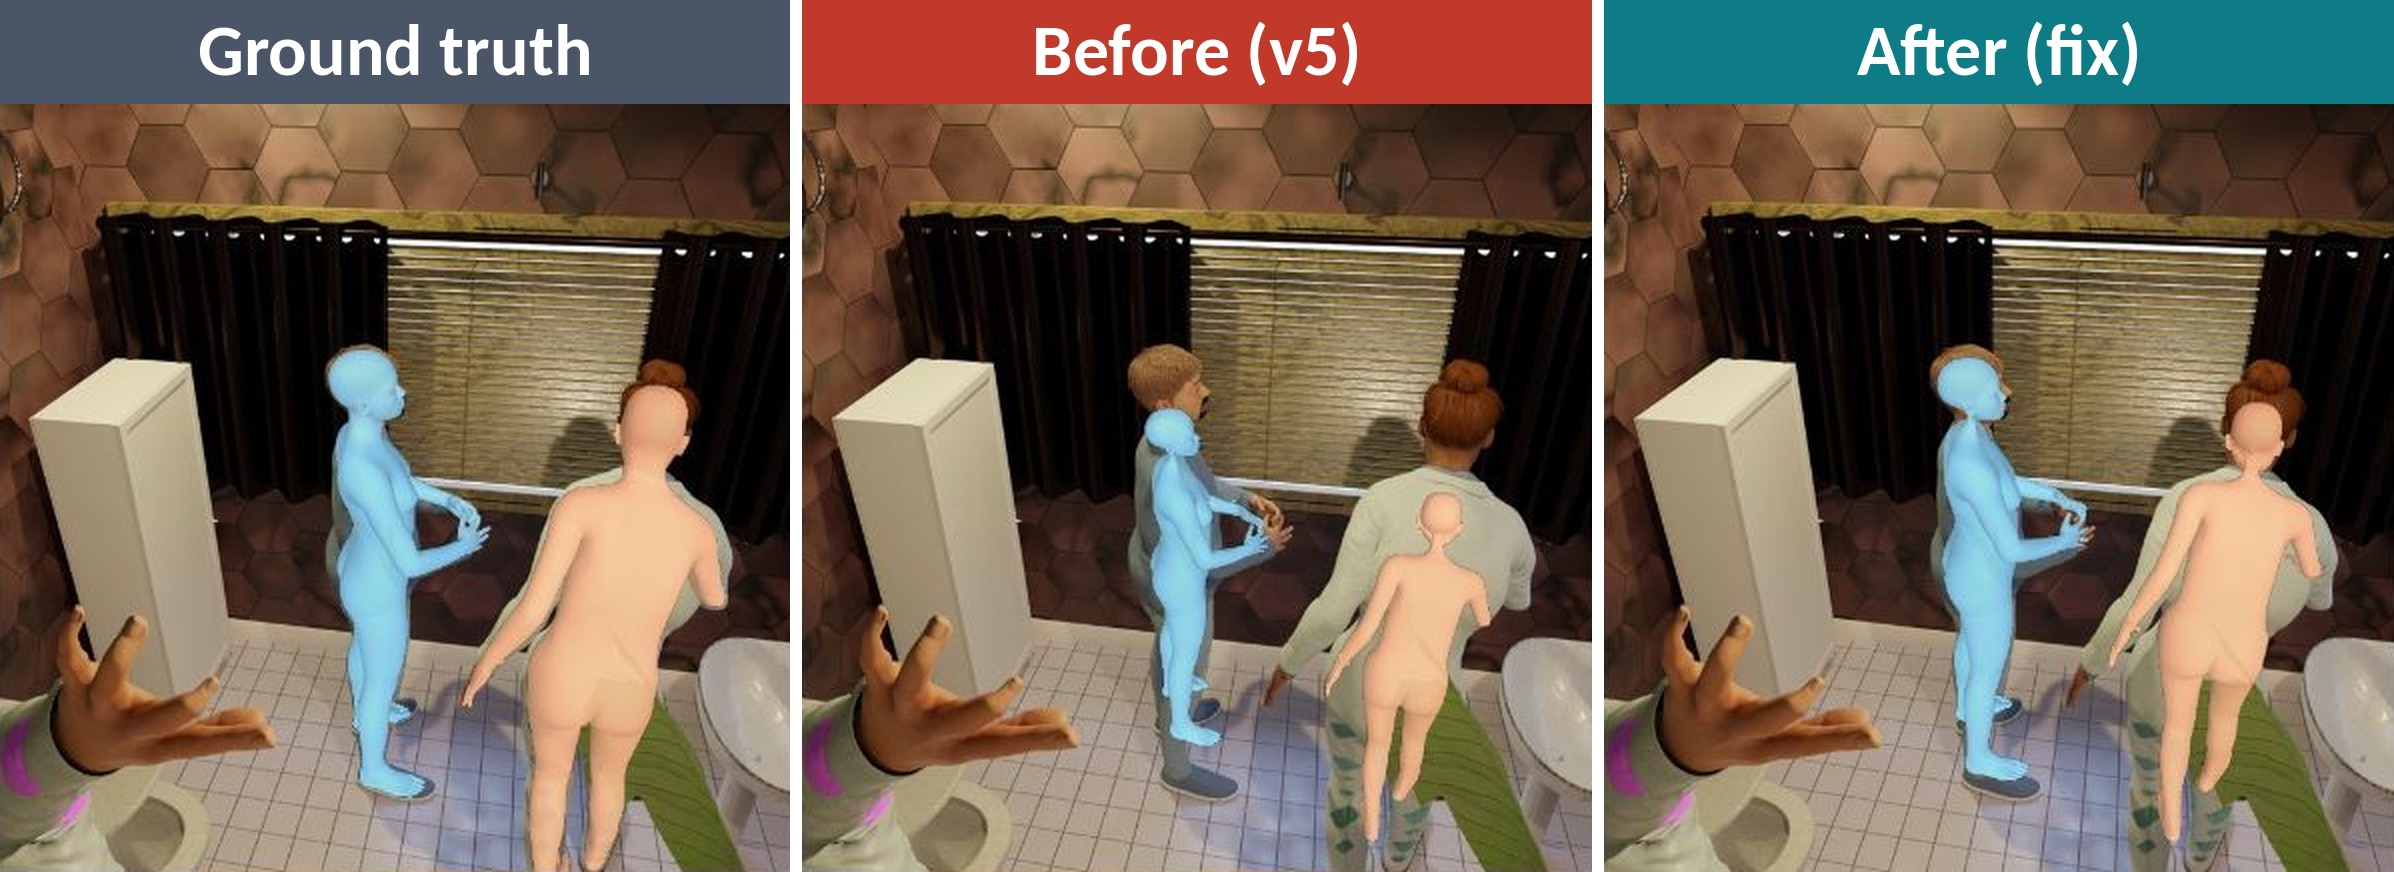
\includegraphics[width=\linewidth]{depth_before_after_579862}
\caption[Holdout image 579862 at the predicted depth: ground truth, Base, depth-fix pilot]{Holdout image 579862 rendered at each model's own predicted depth: ground truth, Base, and the depth-fix pilot (depth weight $\times$5, 10 epochs). The predicted body goes from 0.76 to 0.95 of its true height. Synthetic image; a good case, not a typical one.}
\label{fig:depth-579862}
\end{figure}
% F15 (also cited by Diagnostics 5.3; input it once, here or there)
% F15 Predicted against true root depth, AnnyOne holdout (100 images), Control and Final, setting V1 (eval, masked),
% each body at its own predicted depth. Generated from data/holdout_per_person_{control,final}.csv (rows with
% variant == V1_eval_masked: one row per matched person) by the scratchpad script thesis_plots/gen.py; numbers also in
% data/plot_stats.md. All points drawn, no subsampling (433 coordinates).
% Fit: least squares, pred = a * true + b (metres).
%   Control: n = 219 people (92 images), a = 0.276, b = 2.661 m, r = 0.46,
%            median |pred - true| = 1.237 m (mean 1.268), predicted too far for 99.1%,
%            mean root error 1402 mm (median 1312); fit meets identity at 3.67 m.
%   Final:   n = 214 people (89 images), a = 0.419, b = 1.746 m, r = 0.56,
%            median |pred - true| = 0.626 m (mean 0.654), predicted too far for 94.4%,
%            mean root error 728 mm (median 654); fit meets identity at 3.01 m.
%   Handover reference slopes: Final 0.42, Control 0.28, Base 0.33 (Base intercept 2.36 m). Final and Control agree
%   with the handover to two decimals. Base is not drawn: its per-person CSV has not arrived.
%   n is the number of matched people (detections), below the 222 ground-truth people of the 100 images.
% Needs: pgfplots (compat 1.18). Colours defined locally.
\definecolor{plFinal}{HTML}{2A78D6}% blue: Final
\definecolor{plControl}{HTML}{EB6834}% orange: Control
\definecolor{plBase}{HTML}{7A7A76}% grey: Base
\definecolor{plMasked}{HTML}{1BAF7A}% aqua: Final-masked
\begin{tikzpicture}
\begin{axis}[
  width=0.62\linewidth, height=0.62\linewidth,
  xlabel={true depth (m)}, ylabel={predicted depth (m)},
  xmin=0, xmax=4.5, ymin=0, ymax=4.5, axis equal image,
  xtick={0,1,...,4}, ytick={0,1,...,4},
  grid=major, grid style={gray!20},
  tick label style={font=\footnotesize}, label style={font=\small},
  legend style={font=\footnotesize, at={(0.97,0.03)}, anchor=south east, cells={anchor=west}, draw=gray!50},
  legend cell align=left,
]
% Control, n = 219
\addplot[only marks, mark=square*, mark size=1.1pt, color=plControl, fill opacity=0.55, draw opacity=0.8] coordinates {
(2.107,3.001) (2.404,3.231) (1.921,3.007) (1.070,3.171) (2.425,3.304) (1.849,3.015) (2.698,3.239) (1.862,3.159)
(3.748,3.283) (2.458,3.507) (3.637,3.213) (1.850,3.235) (1.956,3.103) (1.441,2.610) (1.353,2.811) (2.475,3.265)
(2.260,3.166) (2.023,2.824) (1.852,3.120) (1.287,3.298) (2.020,3.271) (1.767,3.185) (2.001,3.187) (1.918,2.972)
(2.384,3.054) (2.145,2.985) (2.696,3.411) (2.084,3.553) (1.991,3.242) (2.452,3.276) (2.369,3.093) (1.306,3.485)
(1.775,2.746) (1.711,2.579) (2.552,3.167) (1.742,3.064) (1.561,3.011) (1.897,3.361) (1.317,3.421) (1.762,3.303)
(1.089,3.256) (1.878,3.075) (1.477,2.770) (2.536,3.448) (2.245,3.395) (1.453,3.400) (2.363,2.995) (2.062,3.202)
(0.988,2.974) (2.242,3.412) (1.887,3.468) (1.939,3.281) (2.078,3.349) (1.603,3.491) (1.429,3.194) (2.451,3.291)
(2.044,3.355) (2.535,3.168) (2.173,3.157) (1.430,3.148) (1.373,2.736) (1.952,3.429) (1.421,3.296) (2.539,3.450)
(2.299,3.301) (2.138,3.173) (1.551,3.034) (1.004,2.652) (1.915,2.860) (1.911,3.022) (2.576,3.361) (2.322,3.171)
(1.932,3.274) (1.551,3.117) (1.834,3.322) (1.476,3.340) (1.325,3.173) (2.272,3.209) (1.983,3.322) (1.371,3.095)
(1.554,3.328) (1.867,3.209) (2.134,3.385) (2.472,3.298) (2.364,3.554) (2.040,3.516) (1.459,3.390) (1.355,3.513)
(2.106,3.086) (1.448,3.288) (2.245,3.064) (2.083,3.303) (1.625,3.278) (1.084,3.125) (2.100,3.542) (1.894,3.132)
(2.003,3.381) (1.052,3.143) (1.344,3.317) (2.255,3.234) (1.518,3.763) (1.404,3.511) (2.239,3.168) (2.108,2.922)
(1.463,2.860) (1.548,2.962) (2.405,3.153) (2.060,3.160) (1.949,3.187) (1.423,3.151) (2.342,3.208) (2.134,2.992)
(1.493,2.899) (1.681,3.030) (1.345,2.972) (2.150,3.159) (2.381,3.235) (2.639,3.141) (1.735,3.140) (1.464,3.225)
(2.308,3.188) (1.983,2.863) (1.676,2.927) (1.333,2.779) (1.338,2.845) (2.332,3.940) (1.730,4.042) (3.423,3.879)
(2.657,3.530) (2.240,3.369) (3.193,3.666) (2.764,3.780) (2.525,3.924) (2.962,3.726) (3.318,3.860) (3.264,3.973)
(2.712,3.959) (1.358,3.071) (1.310,3.500) (2.445,3.691) (2.500,3.581) (1.906,3.607) (1.626,3.088) (1.818,2.943)
(1.813,2.967) (1.980,3.165) (2.070,3.076) (2.550,3.567) (2.045,3.781) (1.559,2.665) (1.159,2.560) (2.187,3.703)
(1.782,3.538) (1.733,2.572) (1.377,2.939) (0.587,2.275) (2.259,2.956) (2.165,3.429) (1.172,2.694) (1.588,2.596)
(1.512,2.661) (0.650,2.569) (2.045,3.056) (1.680,2.828) (1.112,2.721) (1.852,3.079) (1.731,2.925) (1.461,3.412)
(1.889,3.011) (1.499,3.660) (2.449,3.254) (2.574,2.917) (2.376,3.588) (2.574,3.430) (1.401,3.395) (1.582,3.431)
(2.625,3.338) (2.395,3.571) (1.327,3.353) (1.809,3.108) (1.532,2.945) (1.276,3.321) (1.665,2.872) (1.407,3.334)
(1.888,2.749) (1.900,3.189) (0.852,2.487) (1.933,2.944) (1.966,3.339) (2.262,3.209) (2.035,3.029) (1.164,2.686)
(1.885,3.420) (2.342,2.911) (1.500,2.603) (1.836,3.300) (2.555,3.072) (2.340,3.463) (1.699,2.724) (1.334,3.495)
(2.392,3.396) (2.504,3.432) (1.834,3.486) (1.758,2.582) (2.787,3.213) (1.409,3.204) (1.717,2.577) (2.784,3.030)
(1.379,2.996) (2.339,2.803) (2.016,3.263) (1.303,2.508) (2.273,3.135) (1.680,2.821) (1.873,3.493) (2.280,3.339)
(2.089,3.472) (1.657,3.514) (2.251,3.640)
};
\addlegendentry{Control (n = 219)}
% Final, n = 214
\addplot[only marks, mark=*, mark size=1.2pt, color=plFinal, fill opacity=0.55, draw opacity=0.8] coordinates {
(2.107,1.806) (2.404,2.530) (1.921,2.316) (1.070,2.491) (2.425,2.811) (1.849,2.519) (2.698,3.007) (1.862,2.911)
(3.748,2.874) (2.458,3.100) (3.637,2.873) (1.956,2.405) (1.850,2.541) (1.441,2.198) (1.353,2.392) (2.475,2.703)
(2.260,2.582) (2.023,2.148) (1.852,2.457) (1.287,2.618) (2.020,2.458) (1.767,2.354) (2.001,2.255) (1.918,2.016)
(2.145,1.886) (2.384,1.991) (2.696,2.797) (2.431,2.744) (1.991,2.660) (2.084,2.950) (2.369,2.425) (2.452,2.624)
(1.306,2.824) (1.711,2.171) (1.775,2.393) (1.742,2.467) (1.561,2.431) (1.897,2.384) (1.317,2.441) (1.762,2.322)
(1.089,2.278) (1.878,2.426) (1.477,2.155) (2.536,2.662) (2.245,2.599) (1.453,2.631) (2.363,2.023) (2.062,2.201)
(0.988,2.006) (2.242,2.516) (1.887,2.545) (2.078,2.412) (1.939,2.340) (1.429,2.272) (1.603,2.563) (2.451,2.544)
(2.044,2.610) (2.535,2.495) (2.173,2.496) (1.430,2.487) (1.089,2.677) (1.373,2.041) (1.952,3.078) (2.539,2.939)
(2.299,2.788) (2.138,2.454) (1.551,2.309) (1.004,1.948) (1.915,2.378) (1.911,2.538) (2.576,3.020) (2.322,2.830)
(1.932,2.409) (1.551,2.241) (1.834,2.771) (1.476,2.766) (2.272,2.556) (1.983,2.665) (1.371,2.448) (1.867,2.591)
(2.134,2.669) (2.472,2.684) (2.364,2.931) (2.040,2.898) (1.355,2.889) (1.459,2.768) (1.946,2.090) (2.106,1.826)
(1.448,2.074) (2.245,2.418) (2.083,2.672) (1.625,2.620) (1.084,2.477) (0.881,2.592) (1.894,2.240) (2.100,2.602)
(2.003,2.478) (1.052,2.239) (1.344,2.413) (2.255,2.576) (1.949,2.703) (1.518,2.987) (1.404,2.851) (2.108,2.550)
(2.239,2.802) (1.463,2.496) (1.548,2.585) (2.405,2.683) (2.060,2.718) (1.949,2.718) (1.423,2.689) (2.134,2.511)
(2.342,2.759) (1.493,2.432) (1.681,2.564) (1.345,2.490) (2.639,2.912) (2.381,3.006) (2.150,2.915) (1.735,2.900)
(1.464,2.976) (2.308,2.496) (1.676,2.236) (1.983,2.090) (1.338,2.144) (3.423,3.689) (2.657,3.399) (3.193,3.493)
(2.240,3.226) (2.525,3.473) (3.587,3.374) (2.764,3.366) (2.962,3.262) (3.264,3.733) (2.712,3.728) (1.358,2.178)
(2.444,3.111) (2.500,2.865) (1.907,2.637) (1.626,2.639) (1.819,2.590) (1.813,2.622) (1.980,2.849) (2.071,2.853)
(2.550,2.883) (2.045,2.654) (1.559,2.188) (1.159,2.122) (2.187,2.919) (1.733,1.774) (1.377,2.153) (0.587,1.480)
(2.259,2.161) (2.165,2.661) (1.172,1.921) (1.512,1.700) (1.588,1.624) (0.650,1.498) (2.045,2.434) (1.680,2.263)
(1.112,2.138) (1.852,2.645) (1.731,2.143) (1.461,2.636) (1.889,2.687) (1.499,3.350) (2.574,2.825) (2.449,3.080)
(2.574,2.910) (2.376,3.090) (1.401,2.869) (2.625,2.861) (2.395,3.117) (1.809,2.174) (1.532,2.043) (1.276,2.397)
(1.665,1.983) (1.407,2.469) (1.888,1.914) (1.900,2.331) (0.852,1.661) (1.933,2.066) (1.966,2.447) (2.262,2.495)
(2.035,2.154) (1.885,2.560) (1.164,1.853) (2.342,2.474) (1.500,2.149) (1.836,2.883) (2.555,2.430) (2.340,2.868)
(1.699,2.118) (1.334,2.857) (2.392,2.928) (2.504,2.948) (1.834,3.012) (2.787,2.981) (1.758,2.504) (1.409,3.076)
(2.784,2.835) (1.717,2.400) (1.379,2.799) (2.339,2.280) (2.016,2.782) (1.303,1.995) (2.273,2.424) (1.680,2.108)
(1.873,2.818) (1.383,2.889) (2.280,2.620) (2.089,2.735) (2.251,2.895) (1.657,2.779)
};
\addlegendentry{Final (n = 214)}
\addplot[domain=0.587:3.748, samples=2, very thick, color=plControl!80!black, dashed] {0.2757*x + 2.6607};
\addlegendentry{Control fit, slope 0.28}
\addplot[domain=0.587:3.748, samples=2, very thick, color=plFinal!80!black] {0.4195*x + 1.7462};
\addlegendentry{Final fit, slope 0.42}
\addplot[domain=0:4.5, samples=2, densely dotted, thick, black!70] {x};
\addlegendentry{identity}
\end{axis}
\end{tikzpicture}


\section{Bone correction: zero-training, fine-tuned, final}
\label{sec:res-bone}
% absorbs draft main.tex lines 1006-1045 (only the four eliminations survive, as "what is not the cause", in Chapter 5; the LBS conclusion is deleted)
% needs: T9 (Diagnostics writer), F6, F9; girth 0.46 -> 1.00; head direction 19.1 (no training) -> 14.4 -> 13.1 (3579014:113; 3611336:200). Rules: "no sign of a PVE cost", never "PVE improved"; the correction "adds no parameters", "its origin is unknown"
\TODO{The correction without training, after a 2-epoch fine-tune, and in Final.}
% F6 (neck_before_after_v5.jpg) is placed in Chapter 5 (label fig:neck-before-after-v5); refer to it, do not place it twice.
% F9 (plan section 3; caption must say "fine-tuned 2 epochs with the fix", H 9). Office pair in Appendix D.
\begin{figure}[tbp]
\centering
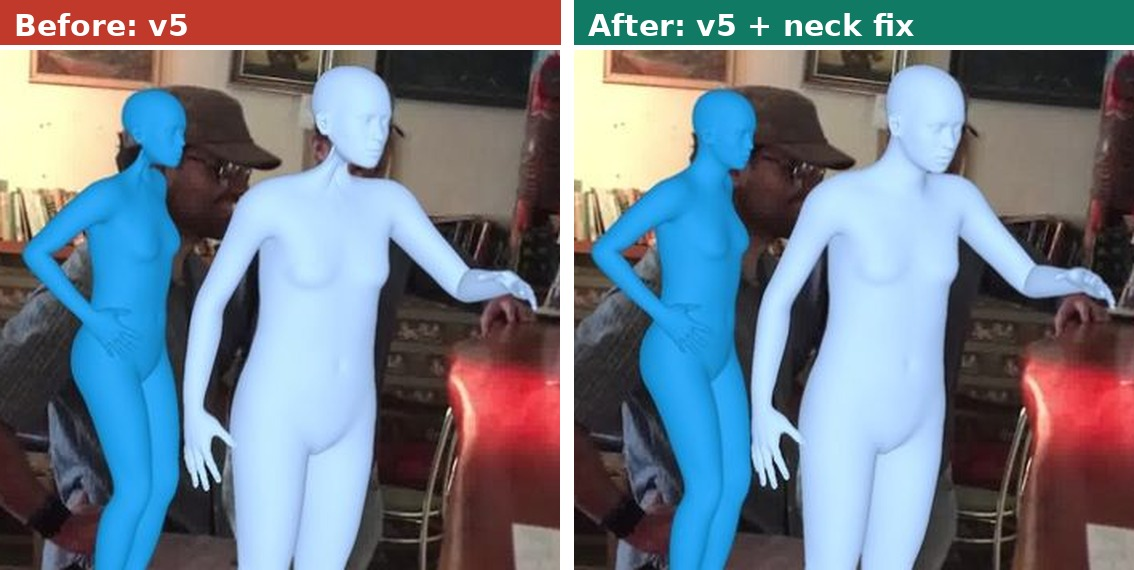
\includegraphics[width=0.85\linewidth]{neck_before_after_3dpw_bar}
\caption[3DPW test frame: Base vs bone correction with a 2-epoch fine-tune]{Real 3DPW test frame \texttt{downtown\_bar\_00} 701: Base next to the model fine-tuned for 2 epochs with the bone correction; bodies placed from the detector box; judged by eye, no metric. The two columns also differ by the fine-tune.}
\label{fig:neck-3dpw-bar}
\end{figure}

\section{Fingers}
\label{sec:res-fingers}
% absorbs - (new; draft line 946 claimed demos show neck elongation on all)
% needs: T10 (Diagnostics writer), F11 (pending); 17.3 -> 8.2 / 8.3 deg (3579014:114; 3611336:201). Rule: "predicted fingers have not been shown on a real photo" until F11 exists
\TODO{Finger angles before and after the correction; no real-photo render yet.}
% F11: cluster demo with --relax_hands 0 (plan section 3 command)
\begin{figure}[tbp]
\centering
\fbox{\parbox[c][3cm][c]{0.8\linewidth}{\centering\TODO{F11 pending: cluster demo with -{}-relax\_hands 0 (plan section 3 command)}}}
\caption{Predicted fingers on the 12 demo images, Final with predicted (not rest-pose) fingers next to Base.}
\label{fig:fingers-demo}
\end{figure}

\section{Final model vs Control vs Base on AnnyOne}
\label{sec:res-final}
% absorbs draft main.tex lines 665-694 (the 145 -> 73.6 -> 74.3 history moves to Section~\ref{sec:res-history} as a V0 table)
% needs: T15 part A, F12 (pending), F20; 73.7 / 50.3 / 87.0 vs 77.4 / 56.4 / 89.0 vs 70.5 / 53.3 / 90.2 (H 5/7); what is inside noise (PVE -3.7) and what is not (PA-PVE -6.1, root -48%); recall cost -2 / -3.2
\TODO{The full V1 table and its reading against the noise floor.}
% T15 Final model vs Control vs Base (Results 6.5-6.6). Owner: Results writer.
% Source: REWRITE_PLAN.md section 4 (T15); H 5/7 table; H 0b 3DPW table.
% Part A: 3570222:40 (Base), long_pc_dist5 = 3572482 (depth pilot, x5, 10 epochs), exp6 fine-tune = 3579014
% (neck pilot), 3611339:182-198 (Control), 3611336:191-207 (Final).
% Part B: 3612073 (Base), 3612074 (Mixed-L old labels = v9 e62), 3612075 (neck pilot), 3611339:215-220,
% 3611336:224-229, 3614192 (NAVER); lines :117-124 for the 3612073-5 jobs.
% Old-label 3DPW numbers (119.1 / 102.5 / 111.5) are retired and never appear next to these.
\begin{table}[tbp]
\centering\footnotesize
\setlength{\tabcolsep}{3pt}
\begin{subtable}{\linewidth}
\centering
\begin{tabular}{@{}lrrrrr@{}}
\toprule
 & Base & \shortstack[r]{Depth\\pilot} & \shortstack[r]{Neck\\pilot} & Control & Final \\
\midrule
PVE (mm) & \BasePVE & 74.8 & 68.8 & \ControlPVE & \FinalPVE \\
PA-PVE (mm) & \BasePAPVE & 54.0 & 50.9 & \ControlPAPVE & \textbf{\FinalPAPVE} \\
Recall (\%) & \BaseRecall & 87.8 & 89.4 & \ControlRecall & \FinalRecall \\
Root error (mm) & \BaseRootErr & \DepthPilotRootErr & 1429 & \ControlRootErr & \textbf{\FinalRootErr} \\
Depth slope & \BaseSlope & 0.38 & 0.34 & \ControlSlope & \FinalSlope \\
Depth intercept (m) & \BaseIntercept & 1.59 & 2.56 & \ControlIntercept & \FinalIntercept \\
Size ratio & \BaseSize & 0.84 & 0.58 & \ControlSize & \FinalSize \\
Neck girth pred/GT & \BaseGirth & 0.457 & 0.997 & \ControlGirth & \FinalGirth \\
PVE\textsubscript{neck} (mm) & 27.3 & 27.7 & 10.7 & \ControlNeckSkin & \FinalNeckSkin \\
Global head direction (deg) & \BaseHeadDir & 12.7 & \NeckPilotHeadDir & \ControlHeadDir & \FinalHeadDir \\
Fingers (deg) & \BaseFingers & 17.4 & 8.3 & \ControlFingers & \FinalFingers \\
neck02 bone (deg) & \BaseNeckTwo & 175.5 & 4.7 & \ControlNeckTwo & \FinalNeckTwo \\
head bone (deg) & 177.9 & 178.0 & 11.2 & \ControlHeadBone & \FinalHeadBone \\
\bottomrule
\end{tabular}
\caption{AnnyOne holdout, 100 images, setting V1 (helper bones masked, matched people); root error, depth fit and size ratio with each body at the model's own predicted depth.}
\label{tab:final-annyone}
\end{subtable}

\vspace{1em}
\begin{subtable}{\linewidth}
\centering
\begin{tabular}{@{}lrrrrrr@{}}
\toprule
 & Base & Mixed-L & \shortstack[r]{Neck\\pilot} & Control & Final & \shortstack[r]{Multi-HMR-\\Anny} \\
\midrule
PVE (mm) & \BaseThreeDPW & \BaseOldThreeDPW & \NeckPilotThreeDPW & \ControlThreeDPW & \textbf{\FinalThreeDPW} & \NAVERThreeDPW \\
PA-PVE (mm) & \BasePAThreeDPW & \BaseOldPAThreeDPW & 68.7 & \ControlPAThreeDPW & \textbf{\FinalPAThreeDPW} & \NAVERPAThreeDPW \\
MPJPE (mm)$^{b}$ & 126.9 & 94.8 & 124.8 & \ControlMPJPEThreeDPW & \textbf{\FinalMPJPEThreeDPW} & \NAVERMPJPEThreeDPW \\
Precision (\%) & \BasePrecThreeDPW & \BaseOldPrecThreeDPW & 53 & 62 & \FinalPrecThreeDPW & \NAVERPrecThreeDPW \\
Recall (\%) & 100 & \BaseOldRecallThreeDPW & 100 & 99 & \FinalRecallThreeDPW & \NAVERRecallThreeDPW \\
\addlinespace
AnnyOne test-100 PVE$^{c}$ & \BaseVzeroPVE & \BaseOldVzeroPVE & 72.7 & 81.2 & \FinalTestHundredPVE & (\NAVERAnnyOne)$^{a}$ \\
\bottomrule
\end{tabular}
\caption{3DPW test, corrected (v23) labels, all 8,190 images, setting V0, same evaluation script for every model. Mixed-L was trained on the labels before their correction and is tested on the corrected ones, like every model here.}
\label{tab:final-3dpw}
\end{subtable}
\caption[Final against Control and Base on the AnnyOne holdout and the 3DPW test]{Final against its Control and against Base. One run per model, no seed; two identical runs differed
by \NoisePVE\,mm PVE, so the PVE gap between Control and Final (\ControlPVE{} vs \FinalPVE) is within run-to-run
variation, while PA-PVE, root error, neck and fingers are not. Depth pilot: depth fix, depth weight $\times$5, 10 epochs;
neck pilot: bone correction and a 2-epoch fine-tune. 3DPW numbers are against our converted labels and are not
comparable with published 3DPW results. $^{a}$Multi-HMR-Anny masks the helper bones by design, so its number is V1 and
compares with Final's \FinalPVE{} in (a); it was most likely trained on these 100 images. $^{b}$Mean over all 163 Anny
joints, pelvis-centred. $^{c}$The same 100 images as (a) in setting V0 (helper bones unmasked).}
\label{tab:final}
\end{table}

% F20 In-training PVE per epoch, Final and Control, epochs 1-10 (one run each, no seed).
% Left: 3DPW-Anny validation (300 images, corrected v23 labels). Right: AnnyOne holdout as evaluated during training
% (setting V0, as train.py prints it; NOT the V1 trace numbers 73.7 / 77.4 mm).
% Data: data/val_curves_exp7.csv (columns final_3dpwval_pve, control_3dpwval_pve, final_holdout_pve,
% control_holdout_pve), written inline; all 40 values drawn. Generated by the scratchpad script thesis_plots/gen.py.
%   3DPW val, Final:   min 73.4 (epoch 7), last 74.5, mean over epochs 75.69
%   3DPW val, Control: min 75.5 (epoch 4), last 75.9, mean over epochs 77.72
%   holdout V0, Final:   min 78.9 (epoch 9), last 79.3, mean over epochs 80.73
%   holdout V0, Control: min 76.8 (epoch 9), last 81.2, mean over epochs 79.19
% Needs: pgfplots (compat 1.18) with \usepgfplotslibrary{groupplots}. Colours defined locally.
\definecolor{plFinal}{HTML}{2A78D6}% blue: Final
\definecolor{plControl}{HTML}{EB6834}% orange: Control
\definecolor{plBase}{HTML}{7A7A76}% grey: Base
\definecolor{plMasked}{HTML}{1BAF7A}% aqua: Final-masked
\begin{tikzpicture}
\begin{groupplot}[
  group style={group size=2 by 1, horizontal sep=1.6cm},
  width=0.5\linewidth, height=5cm,
  xmin=0.5, xmax=10.5, xtick={1,...,10}, xlabel={epoch},
  ylabel={PVE (mm)},
  grid=major, grid style={gray!20},
  tick label style={font=\footnotesize}, label style={font=\small}, title style={font=\small},
]
\nextgroupplot[title={3DPW validation}, ymin=72, ymax=84,
  legend style={font=\footnotesize, at={(0.97,0.97)}, anchor=north east, draw=gray!50}, legend cell align=left]
\addplot[color=plControl, mark=square*, mark size=1.6pt, thick, dashed, mark options={solid}] coordinates {(1,80.6) (2,76.1) (3,80.9) (4,75.5) (5,77.2) (6,78.2) (7,77.4) (8,76.7) (9,78.7) (10,75.9)};
\addlegendentry{Control}
\addplot[color=plFinal, mark=*, mark size=1.7pt, thick] coordinates {(1,79.9) (2,75.7) (3,77.8) (4,74.4) (5,75.5) (6,75.0) (7,73.4) (8,75.4) (9,75.3) (10,74.5)};
\addlegendentry{Final}
\nextgroupplot[title={AnnyOne holdout (in training)}, ymin=72, ymax=84]
\addplot[color=plControl, mark=square*, mark size=1.6pt, thick, dashed, mark options={solid}] coordinates {(1,79.3) (2,77.7) (3,77.7) (4,79.8) (5,79.4) (6,78.2) (7,83.2) (8,78.6) (9,76.8) (10,81.2)};
\addplot[color=plFinal, mark=*, mark size=1.7pt, thick] coordinates {(1,81.1) (2,80.2) (3,80.1) (4,80.8) (5,81.6) (6,82.3) (7,81.1) (8,81.9) (9,78.9) (10,79.3)};
\end{groupplot}
\end{tikzpicture}

% F12: trace panels stacked on the cluster (plan section 3 command)
\begin{figure}[tbp]
\centering
\fbox{\parbox[c][3cm][c]{0.8\linewidth}{\centering\TODO{F12 pending: trace panels stacked on the cluster (plan section 3 command)}}}
\caption{Six holdout images: photo, ground truth, Base, Final, each at its own predicted depth.}
\label{fig:holdout-montage}
\end{figure}

\section{3DPW test on the corrected labels}
\label{sec:res-3dpw}
% absorbs draft main.tex lines 1131-1221 (old-label numbers retired; validation-trajectory text moves to history)
% needs: T15 part B, F10 (pending); 121.8 / 95.5 / 120.2 / 91.5 / 89.0 (3612073-5; 3611339; 3611336); most of the gain is training on 3DPW (Control 91.5); the fixes add 2.5 mm; precision 64% explained (bystanders not labelled). Wording: "lowest error on our 3DPW-Anny labels", "not comparable with published 3DPW numbers"
\TODO{Every model on the v23 test labels with the same script.}
% F10 (plan section 3): demo job 3612078 montages, each photo | Base | photo | Final, labels baked in
% (data/CLUSTER_ANSWERS.md). 3 of the 8 3DPW frames received; missing: downtown_bar, downtown_walking,
% downtown_sitOnStairs, downtown_walkBridge, weekly market.
\begin{figure}[tbp]
\centering
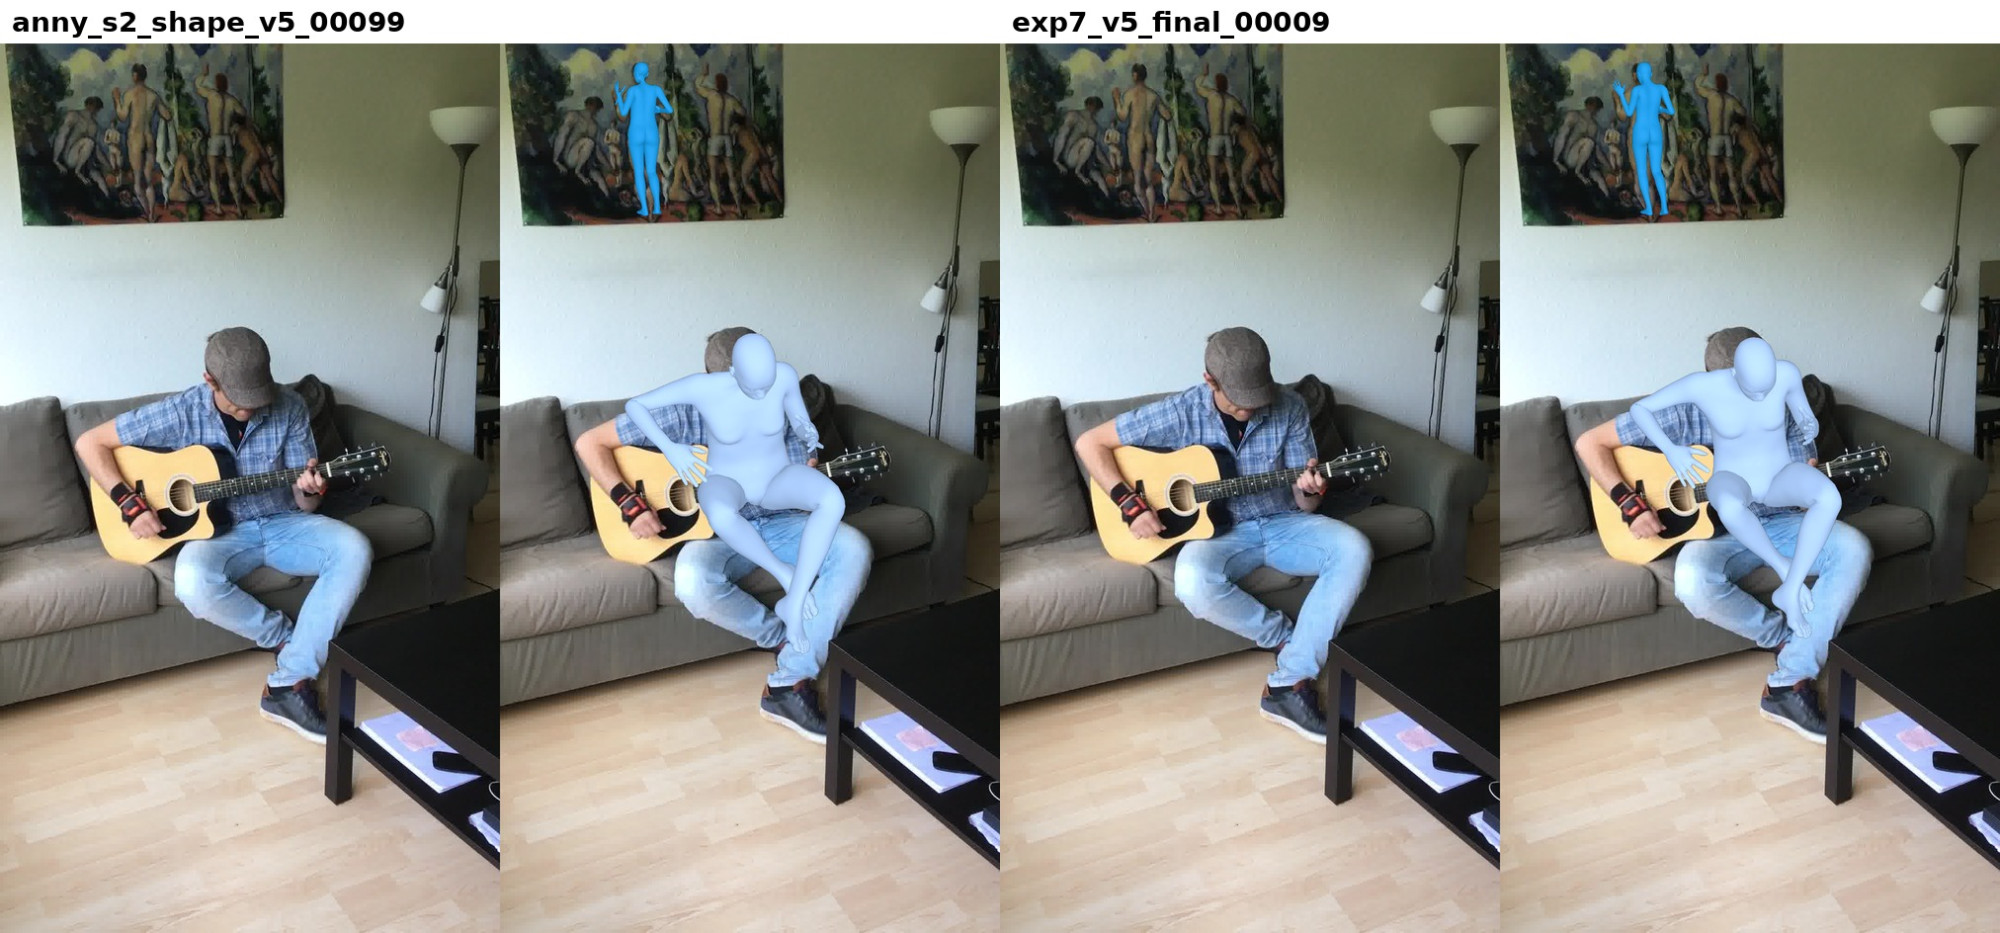
\includegraphics[width=\linewidth]{F10_3dpw_guitar_v5_vs_final}\\[2pt]
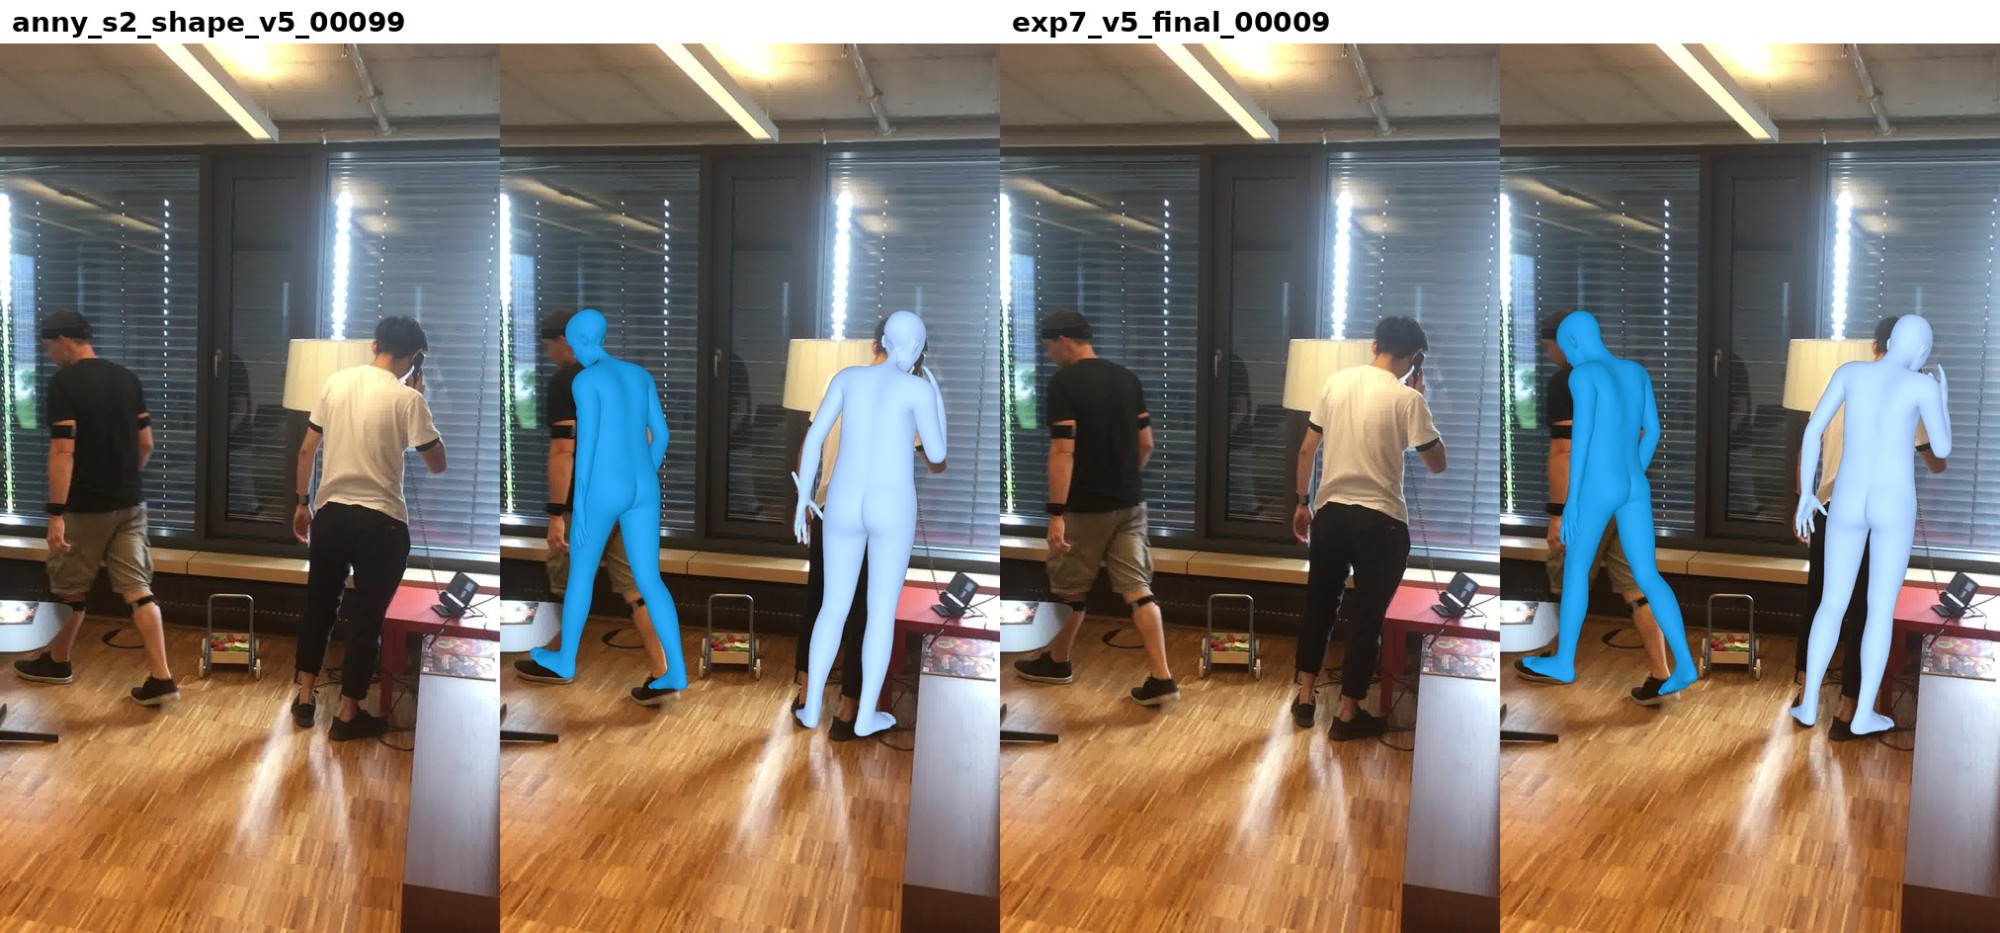
\includegraphics[width=\linewidth]{F10_3dpw_office_v5_vs_final}\\[2pt]
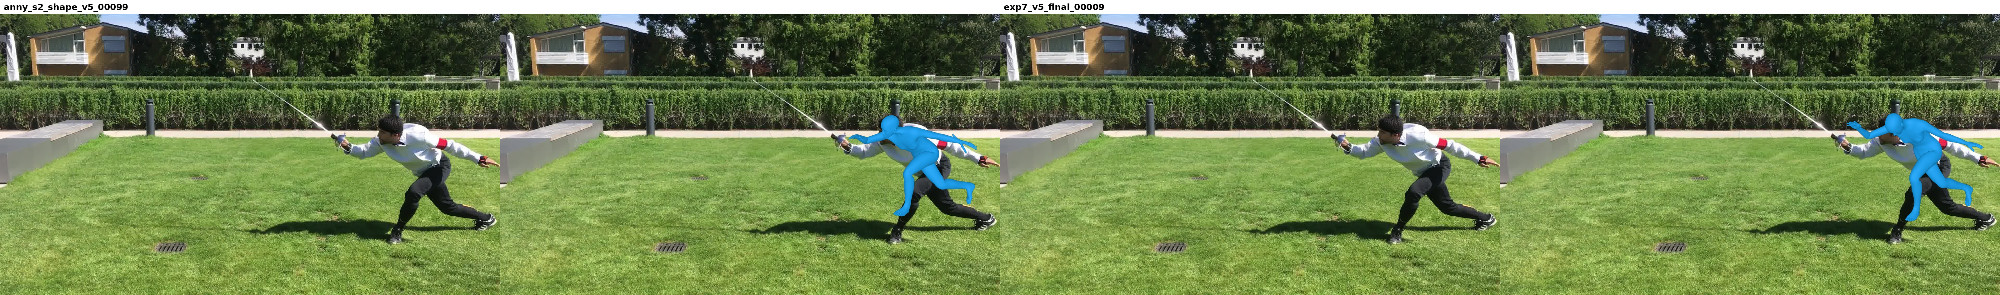
\includegraphics[width=\linewidth]{F10_3dpw_fencing_v5_vs_final}
\caption[3DPW test frames, Base vs Final]{3DPW test frames, each shown as photo and Base, then photo and Final; bodies placed from the detector box; judged by eye, no metric. \TODO{five more frames pending}}
\label{fig:3dpw-overlays}
\end{figure}

\section{Real photos: Relative Human and the demo}
\label{sec:res-rh}
% absorbs - (new)
% needs: T12, F13, F16, F17 (pending); gender 46.5 -> 64.2; AUC 0.61 -> 0.72; babies 0.44 vs adults 0.54; recall 47 -> 65; by-eye reading of the 12 images. Rule: children "a measured improvement, not solved"; never convert Anny ages to years
\TODO{Relative Human numbers and the by-eye reading of the demo images.}
% T12 Relative Human (Results 6.7 / 6.8). Owner: Results writer.
% Source: REWRITE_PLAN.md section 4 (T12); H 0a "DECIDED"; H 0b; H 3.4.
% Base = 3611285_0 (:23-31), Final = 3612131 (:25-33), Final-masked = 3613616 (logs/eval_rh_3613616_0.out).
% Demo spread: jobs 3612078 (Final) vs 3613617 (Final-masked), 12 images, [shape] lines (H 0a).
% "--" = not reported in the sources.
\begin{table}[tbp]
\centering\small
\begin{tabular}{@{}lrrr@{}}
\toprule
 & Base & Final & Final-masked \\
\midrule
Recall (\%) & \RHRecallBase & \RHRecallFinal & \RHRecallMasked \\
Gender accuracy (\%) & \RHGenderBase & \RHGenderFinal & \RHGenderMasked \\
\quad mean gender, men (male = 0) & 0.535 & 0.551 & 0.717 \\
\quad mean gender, women (female = 1) & 0.551 & 0.861 & 0.860 \\
Child-vs-adult AUC & \RHAUCBase & \RHAUCFinal & \RHAUCMasked \\
\addlinespace
Mean age, adult & 0.631 & 0.536 & 0.638 \\
\quad teen & 0.597 & 0.524 & -- \\
\quad kid & 0.613 & 0.500 & 0.611 \\
\quad baby & 0.624 & 0.438 & 0.524 \\
Babies with age $<$ 0.45 (\%) & 2.6 & 49.3 & 16.9 \\
Mean height, adult & 0.507 & 0.500 & -- \\
\quad kid & 0.451 & 0.466 & -- \\
\quad baby & 0.394 & 0.464 & -- \\
Matched children + adults & 948 & 1,305 & -- \\
\midrule
\multicolumn{4}{@{}l}{\emph{Demo images: standard deviation of the prediction}} \\
Muscle & -- & 0.04 & 0.06 \\
Weight & -- & 0.04 & 0.11 \\
Cup size & -- & 0.05 & 0.11 \\
Firmness & -- & 0.04 & 0.11 \\
Age & -- & 0.03 & 0.08 \\
\bottomrule
\end{tabular}
\caption{Body shape on real photos. Upper part: Relative Human validation split (635 images, 2,130 labelled people),
detected people only, matched to the labelled boxes at IoU $\geq$ 0.3; ``child'' means a predicted age below 0.45;
the matched sets differ between models because recall differs. Lower part: spread of the predicted phenotypes over all
detected people of the 12 demo images (4 photos and 8 3DPW test frames), not matched to people. The neck pilot
(bone correction and a 2-epoch fine-tune) is the same as Base within run-to-run variation (AUC 0.613).}
\label{tab:relhuman}
\end{table}

% F13 (plan section 3). Source docs/figures/final_model_real_photos.jpg (labels baked in).
\begin{figure}[tbp]
\centering
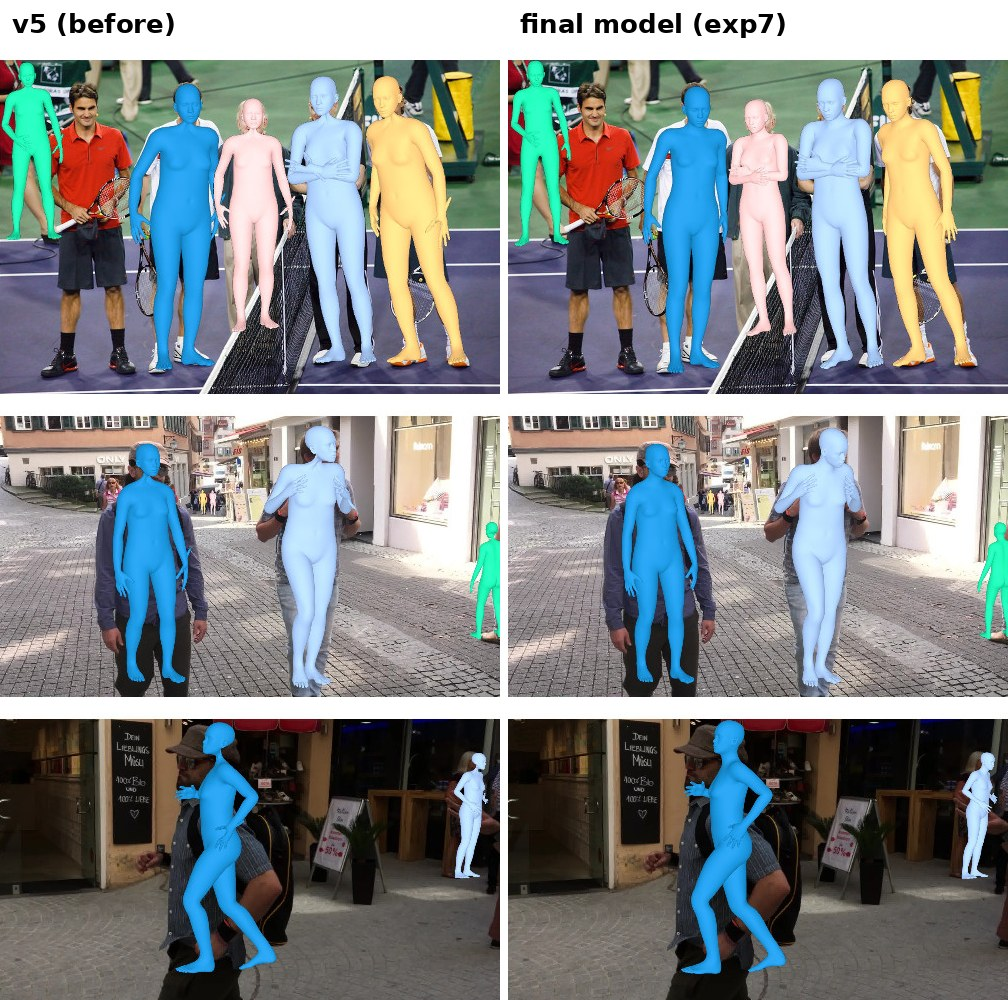
\includegraphics[width=0.8\linewidth]{final_model_real_photos}
\caption[Three real photos, Base vs Final]{Three real photos, Base (left) and Final (right), bodies placed from the detector box: most men get male bodies, women stay female, the boy stays an adult body. Judged by eye; no metric exists for these images.}
\label{fig:real-photos}
\end{figure}
% F16 Predicted Anny age per Relative Human group (adult, teen, kid, baby) for Base and Final, with the child
% threshold 0.45 (Results 6.7). PLACEHOLDER: data pending.
% Waits for (REWRITE_PLAN.md section 3 "F15 and F16, CSVs"; section 7 Q11):
%   data/F16_rh_base.csv    <- results/diagnostics/relative_human_val_anny_s2_shape_v5_00099/per_person.csv
%   data/F16_rh_final.csv   <- results/diagnostics/relative_human_val_exp7_v5_final_00009/per_person.csv
%   data/F16_rh_masked.csv  <- the masked arm's per_person.csv (optional third model)
% Column names known (data/CLUSTER_ANSWERS.md): age_group, pred_age, matched (keep matched rows).
% Then one \addplot[boxplot] table[y=pred_age] per age_group and model (pgfplots statistics library is loaded).
\begin{figure}[tbp]
\centering
\begin{tikzpicture}
\begin{axis}[
  width=0.8\linewidth, height=5.5cm,
  ylabel={Predicted Anny age}, ymin=0, ymax=1,
  xmin=0.5, xmax=4.5, xtick={1,2,3,4}, xticklabels={adult, teen, kid, baby},
  grid=major, grid style={gray!25},
  tick label style={font=\footnotesize}, label style={font=\small},
]
\draw[dashed, red!60!black] (axis cs:0.5,0.45) -- (axis cs:4.5,0.45) node[pos=0.01, anchor=south west, font=\scriptsize] {child threshold 0.45};
\node[font=\small\bfseries, red!70!black, align=center] at (axis cs:2.5,0.8) {data pending\\[-1pt]\footnotesize Relative Human per\_person.csv};
\end{axis}
\end{tikzpicture}
\caption{Predicted Anny age per Relative Human age group, Base and Final; detected people only. \TODO{plot pending:
Relative Human per-person CSVs}}
\label{fig:rh-age}
\end{figure}

% F17: cluster demo with --rest_pose 1 (plan section 3 command)
\begin{figure}[tbp]
\centering
\fbox{\parbox[c][3cm][c]{0.8\linewidth}{\centering\TODO{F17 pending: cluster demo with -{}-rest\_pose 1 (plan section 3 command)}}}
\caption{Rest-pose line-up: every detected person of the 12 demo images in rest pose, Final, so only body shape differs.}
\label{fig:rest-lineup}
\end{figure}

\section{The shape-mask trade-off}
\label{sec:res-mask}
% absorbs - (new)
% needs: T12 (masked column and demo spread); variety back (std 0.04 -> 0.11) vs gender back to 49.3% and children weaker; the decision (H 0a "DECIDED"); the partial mask (pending, Final-masked-7)
\TODO{Final-masked against Final: shape variety against gender and children.}

\section{Baseline comparison and model cost}
\label{sec:res-baseline}
% absorbs draft main.tex lines 631-652 (paper table replaced by the measured Multi-HMR-Anny row)
% needs: T16, F18; 60.3 / 126.9 vs 73.7 / 89.0; cost measured: NAVER 380.94 M (head 76.57 M), backbone 1917.2 GFLOPs, ms not measurable for its class; Final 318.38 M, 1927.4 GFLOPs, 77.9 ms (A100) / 110 ms (A40). Fixed wording on the in-sample 60.3 (plan section 5)
\TODO{Multi-HMR-Anny against Final on both sets, with the in-sample caveat; parameters, FLOPs and time.}
% Source macros retain the measured results and provenance in numbers_results.tex.
% Split the former 12-column table for readable reconstruction/cost comparisons.
\begin{table}[!tbp]
\centering\small
\setlength{\tabcolsep}{3pt}
\begin{tabular}{@{}lrrrrrrc@{}}
\toprule
& \multicolumn{3}{c}{AnnyOne holdout (V1)} & \multicolumn{3}{c}{3DPW test (v23)} & \\
\cmidrule(lr){2-4}\cmidrule(lr){5-7}
Model & PVE & PA-PVE & Recall & PVE & PA-PVE & Recall & \shortstack{3DPW\\training} \\
\midrule
Released baseline & \NAVERAnnyOne$^a$ & \NAVERPAAnnyOne$^a$ & \NAVERRecallAnnyOne$^a$ & \NAVERThreeDPW & \NAVERPAThreeDPW & \NAVERRecallThreeDPW & no \\
Teacher (Final) & \FinalPVE & \FinalPAPVE & \FinalRecall & \textbf{\FinalThreeDPW} & \textbf{\FinalPAThreeDPW} & \FinalRecallThreeDPW & yes \\
Student (ViT-B) & \StudentPVE & \StudentPAPVE & \StudentRecall & \StudentThreeDPW & \StudentPAThreeDPW & \StudentRecallThreeDPW & yes \\
Control & \ControlPVE & \ControlPAPVE & \ControlRecall & \ControlThreeDPW & \ControlPAThreeDPW & 99 & yes \\
Base & \BasePVE & \BasePAPVE & \BaseRecall & \BaseThreeDPW & \BasePAThreeDPW & 100 & no \\
\bottomrule
\end{tabular}
\caption[Reconstruction comparison of student and reference models]{Reconstruction comparison. Errors are in mm;
recall is in percent. One checkpoint is evaluated per model; thesis-trained models were not repeated across seeds. 3DPW errors use converted Anny labels and are not
comparable with published SMPL-space results. $^a$The released baseline was trained on the AnnyOne release,
which includes these holdout images, so its synthetic result is potentially in-sample. The real-image
training exposure differs between released baseline and student/teacher.}
\label{tab:baseline}
\end{table}

\begin{table}[!tbp]
\centering\small
\begin{tabular}{@{}lrrrr@{}}
\toprule
Model & Params (M) & GFLOPs & \shortstack{Latency\\L40S (ms)} & \shortstack{Latency\\A100 (ms)} \\
\midrule
Released baseline & \NAVERParams & $\geq$\NAVERBackboneGFLOPs$^b$ & n/m & n/m \\
Teacher (Final) & \FinalParams & \FinalGFLOPs & \TeacherMsLFortyS & \TeacherMsAHundred \\
Student (ViT-B) & \StudentParams & \StudentGFLOPs & \StudentMsLFortyS & n/m \\
\bottomrule
\end{tabular}
\caption[Model size, computation and recorded forward latency]{Model cost at 672\,px input and one person.
One multiply-add counts as two FLOPs. Latency is median batch-one forward time in fp32 with TF32; compare
only within a GPU column. The student/teacher L40S pair was measured in the same job. n/m: not measured.
$^b$The baseline figure counts only its backbone, so total computation is higher. Base and Control share
the teacher architecture; fixed rotation corrections add no trainable parameters.}
\label{tab:model-cost}
\end{table}

% F18 Parameters and GFLOPs against 3DPW-test PVE (Results 6.9). Owner: Results writer.
% Numbers from tables/T16 via numbers_results.tex: NAVER 380.94 M / >= 1917.2 GFLOPs (backbone only,
% head FLOPs not countable for its class; job 3614947) / 126.9 mm; Final 318.38 M / 1927.4 / 89.0 mm;
% Student 101.38 M / 603.3 GFLOPs, PVE pending (job 3614191): drawn as a dashed vertical line until known.
% 19 Oct: the Student's measured point (110.1 mm, job 3614191) replaces the dashed line.
\begin{figure}[!tbp]
\centering
\begin{tikzpicture}
\begin{groupplot}[
  group style={group size=2 by 1, horizontal sep=0.6cm, y descriptions at=edge left},
  width=0.5\linewidth, height=4.8cm,
  ylabel={3DPW test PVE (mm)}, ymin=70, ymax=140,
  grid=major, grid style={gray!25},
  tick label style={font=\footnotesize}, label style={font=\small},
]
\nextgroupplot[xlabel={Parameters (M)}, xmin=0, xmax=450]
  \draw[densely dotted, black!60] (axis cs:0,\BarThreeDPW) -- (axis cs:450,\BarThreeDPW);
  \node[font=\scriptsize, anchor=south east, black!70] at (axis cs:445,\BarThreeDPW) {95\,\% bar};
  \addplot[only marks, mark=square*, color=gray!70!black] coordinates {(\NAVERParams,\NAVERThreeDPW)};
  \node[font=\scriptsize, anchor=north east] at (axis cs:\NAVERParams,\NAVERThreeDPW-2) {Multi-HMR-Anny};
  \addplot[only marks, mark=*, color=blue!70!black] coordinates {(\FinalParams,\FinalThreeDPW)};
  \node[font=\scriptsize, anchor=north, blue!70!black] at (axis cs:\FinalParams,\FinalThreeDPW-2) {Teacher};
  \addplot[only marks, mark=triangle*, mark size=2.5pt, color=red!70!black] coordinates {(\StudentParams,\StudentThreeDPW)};
  \node[font=\scriptsize, anchor=south, red!70!black] at (axis cs:\StudentParams,\StudentThreeDPW+2) {Student};
\nextgroupplot[xlabel={GFLOPs}, xmin=0, xmax=2400]
  \draw[densely dotted, black!60] (axis cs:0,\BarThreeDPW) -- (axis cs:2400,\BarThreeDPW);
  \addplot[only marks, mark=square*, color=gray!70!black] coordinates {(\NAVERBackboneGFLOPs,\NAVERThreeDPW)};
  \draw[->, gray!70!black] (axis cs:\NAVERBackboneGFLOPs,\NAVERThreeDPW) -- (axis cs:\NAVERBackboneGFLOPs+300,\NAVERThreeDPW);
  \node[font=\scriptsize, anchor=north east, align=right] at (axis cs:\NAVERBackboneGFLOPs+250,\NAVERThreeDPW-2) {Multi-HMR-Anny\\(backbone only)};
  \addplot[only marks, mark=*, color=blue!70!black] coordinates {(\FinalGFLOPs,\FinalThreeDPW)};
  \node[font=\scriptsize, anchor=north, blue!70!black] at (axis cs:\FinalGFLOPs,\FinalThreeDPW-2) {Teacher};
  \addplot[only marks, mark=triangle*, mark size=2.5pt, color=red!70!black] coordinates {(\StudentGFLOPs,\StudentThreeDPW)};
  \node[font=\scriptsize, anchor=south, red!70!black] at (axis cs:\StudentGFLOPs,\StudentThreeDPW+2) {Student};
\end{groupplot}
\end{tikzpicture}
\caption[Model size and compute against 3DPW-test PVE]{Model size and compute against 3DPW-test PVE (corrected labels, all 8,190 images; one run per model). Multi-HMR-Anny's GFLOPs count its
backbone only (arrow: the true value is higher). Dotted
line: the retention threshold against the teacher (\BarThreeDPW\,mm).}
\label{fig:cost-pve}
\end{figure}


\section{The ViT-B student}
\label{sec:res-student}
% absorbs draft main.tex lines 1122-1129 (student backbone size; "a ViT-B student was not trained" is deleted)
% needs: T11 (Method writer), T17, F19; recipe recap; teacher / student / ratio / bar; verdict as measured; the 95% rule against both baselines (bars \BarPVE{} / \BarThreeDPW{} and \BarNAVERAnnyOne{} / \BarNAVERThreeDPW). Pending job 3614191
\TODO{The Student against its teacher and the 95\,\% rule (pending).}
% T17 Student result (Results 6.10). Owner: Results writer. Filled 19 Oct from job 3614191 (logs/exp8_distill_vitb_3614191.out;
% data/CLUSTER_ANSWERS.md "STUDENT DONE"): holdout V1 :195-207, cost on an L40S :213-221, final table :259-283.
% The job re-measured the teacher with the same values as below; ratios = student / teacher (recall: student / teacher).
% Earlier note:
% Fill from <RUN>/final_table.json (RUN = student_vitb_from_v5_pc_dist5_bonefix_v23_e10_00009_e30); the job
% re-measures the teacher, so replace the teacher column by the job's values and recompute the bars.
% Teacher values now: V1 3611336:191-193 (PVE, PA-PVE, recall); V1 MPJPE 77.9 = mean of mpjpe over the
% V1_eval_masked rows of data/holdout_per_person_final.csv (its PVE / PA-PVE means reproduce 73.7 / 50.3);
% test-100 V0 and 3DPW 3611336:218-229; cost 3613926 (A40); training throughput 3611336:15 (A100).
% Bars: error metrics teacher / 0.95 (77.6 and 93.7 from H 0a; 52.9, 82.0, 81.6, 57.3, 60.6, 92.9 computed here);
% recall teacher x 0.95 (82.7, 94.1 computed here); cost: the student must be lower.
\begin{table}[!tbp]
\centering\footnotesize
\begin{tabular}{@{}lrrrrc@{}}
\toprule
Metric & Teacher & Student & Ratio & Bar & Met? \\
\midrule
\multicolumn{6}{@{}l}{\emph{AnnyOne holdout, V1}} \\
PVE (mm) & \FinalPVE & \StudentPVE & \StudentRatioPVE & $\leq$ \BarPVE & no \\
PA-PVE (mm) & \FinalPAPVE & \StudentPAPVE & 1.61 & $\leq$ 52.9 & no \\
MPJPE (mm) & \FinalMPJPE & \StudentMPJPE & 1.63 & $\leq$ \BarMPJPE & no \\
Recall (\%) & \FinalRecall & \StudentRecall & 0.98 & $\geq$ 82.7 & yes \\
\addlinespace
\multicolumn{6}{@{}l}{\emph{AnnyOne test-100, V0}} \\
PVE (mm) & \FinalTestHundredPVE & \StudentTestHundredPVE & 1.58 & $\leq$ 81.6 & no \\
PA-PVE (mm) & \FinalTestHundredPAPVE & \StudentTestHundredPAPVE & 1.55 & $\leq$ 57.3 & no \\
Recall (\%) & 87 & \StudentTestHundredRecall & 0.98 & $\geq$ 82.7 & yes \\
\addlinespace
\multicolumn{6}{@{}l}{\emph{3DPW test (v23 labels), V0}} \\
PVE (mm) & \FinalThreeDPW & \StudentThreeDPW & \StudentRatioThreeDPW & $\leq$ \BarThreeDPW & no \\
PA-PVE (mm) & \FinalPAThreeDPW & \StudentPAThreeDPW & 1.25 & $\leq$ 60.6 & no \\
MPJPE (mm) & \FinalMPJPEThreeDPW & \StudentMPJPEThreeDPW & 1.27 & $\leq$ \BarMPJPEThreeDPW & no \\
Recall (\%) & \FinalRecallThreeDPW & \StudentRecallThreeDPW & 1.00 & $\geq$ 94.1 & yes \\
\addlinespace
\multicolumn{6}{@{}l}{\emph{Cost (L40S, batch 1, one person)}} \\
Params (M) & \FinalParams & \StudentParams & \ParamRatioStudent$\times$ & fewer & yes \\
GFLOPs & \FinalGFLOPs & \StudentGFLOPs & \FlopRatioStudent$\times$ & fewer & yes \\
ms per image & \TeacherMsLFortyS & \StudentMsLFortyS & \SpeedRatioStudent$\times$ & faster & yes \\
Training images/s & \FinalTrainImgPerSec$^{a}$ & \StudentTrainImgPerSec$^{a}$ & & & \\
\bottomrule
\end{tabular}
\caption[The Student against its teacher and the 95\,\% rule]{The Student against its teacher (Final) and the
95\,\% rule: every error of the Student at most the teacher's divided by 0.95, every recall at least 0.95 of the
teacher's, and fewer parameters, fewer FLOPs and a faster forward pass. The rule fails on every error and holds on
recall and cost. One run, no seed. Against Multi-HMR-Anny the PVE bars would be \BarNAVERAnnyOne\,mm on AnnyOne
(most likely in-sample for it; not met) and \BarNAVERThreeDPW\,mm on 3DPW (met). Cost: both models timed in the
Student's job on one L40S. $^{a}$Final on an A100, the Student on the L40S; not comparable.}
\label{tab:student}
\end{table}

% F19 The Student's holdout and 3DPW-validation PVE per evaluated epoch next to the teacher's values
% (Results 6.10). PLACEHOLDER: data pending (job 3614191).
% Waits for (REWRITE_PLAN.md section 7 Q2):
%   grep -E "epoch|pve|PVE" results/experiments/exp8_distill_vitb/student_vitb_from_v5_pc_dist5_bonefix_v23_e10_00009_e30/train.log
%   -> data/F19_student.csv (columns: epoch,holdout_pve,val3dpw_pve)
\begin{figure}[tbp]
\centering
\begin{tikzpicture}
\begin{axis}[
  width=0.8\linewidth, height=5.5cm,
  xlabel={Epoch}, ylabel={PVE (mm)}, xmin=0, xmax=30, ymin=60, ymax=140,
  grid=major, grid style={gray!25},
  tick label style={font=\footnotesize}, label style={font=\small},
]
\draw[densely dotted, blue!70!black] (axis cs:0,\FinalPVE) -- (axis cs:30,\FinalPVE) node[pos=0.99, anchor=south east, font=\scriptsize] {teacher, holdout V1 (\FinalPVE)};
\draw[densely dotted, black!60] (axis cs:0,\BarPVE) -- (axis cs:30,\BarPVE) node[pos=0.99, anchor=south east, font=\scriptsize] {95\,\% bar (\BarPVE)};
\node[font=\small\bfseries, red!70!black, align=center] at (axis cs:15,120) {data pending\\[-1pt]\footnotesize Student train.log};
\end{axis}
\end{tikzpicture}
\caption[The Student's error per epoch against the teacher's]{The Student's holdout (V1) and 3DPW-validation PVE per evaluated epoch, against the teacher's holdout value and the 95\,\% bar. One run, no seed. \TODO{plot pending: Student training log}}
\label{fig:student-curves}
\end{figure}


\section{History: the ViT-S students and the v2--v5 schedule}
\label{sec:res-history}
% absorbs draft main.tex lines 665-810 and 1131-1221
% needs: draft tables tab:main (label it V0), tab:kd_eval, tab:kd_epochs (tables/draft_*.tex); old 3DPW table only if re-run on v23 (plan section 7 Q5), else "old labels, retired" or dropped; F22; one paragraph on what they taught
\TODO{The draft's schedule and student tables, labelled V0 and old labels.}
% F22 The ViT-S students' holdout PVE over epochs (Results 6.11, history). Owner: Results writer.
% Numbers: draft tab:kd_epochs (draft_2026-10_original/main.tex:751-768; tables/draft_kd_epochs.tex),
% PVE only, setting V0 (helper bones unmasked, train.py evaluate()). Epoch "best" left out.
% Drawn now because the plan names the draft table as its source (REWRITE_PLAN.md section 3, F22).
\begin{figure}[tbp]
\centering
\begin{tikzpicture}
\begin{axis}[
  width=0.8\linewidth, height=5.5cm,
  xlabel={Epoch}, ylabel={AnnyOne holdout PVE, V0 (mm)},
  xmin=-5, xmax=135, ymin=140, ymax=400, xtick={0,30,60,100,130},
  grid=major, grid style={gray!25},
  tick label style={font=\footnotesize}, label style={font=\small},
  legend style={font=\footnotesize, at={(0.98,0.97)}, anchor=north east}, legend columns=2,
]
\addplot[color=gray, mark=o] coordinates {(0,377) (30,305) (60,228) (100,213) (130,199)};
\addlegendentry{v3}
\addplot[color=orange!80!black, mark=square] coordinates {(0,298) (30,239) (60,197) (100,179) (130,163)};
\addlegendentry{v4}
\addplot[color=green!50!black, mark=triangle] coordinates {(0,378) (30,240) (60,205) (100,175) (130,159)};
\addlegendentry{v5}
\addplot[color=blue!70!black, mark=*, thick] coordinates {(0,327) (30,221) (60,186) (100,175) (130,155)};
\addlegendentry{v6}
\draw[dashed, black!60] (axis cs:-5,193) -- (axis cs:135,193) node[pos=0.02, anchor=south west, font=\scriptsize] {v2 (random heads), final: 193};
\end{axis}
\end{tikzpicture}
\caption{Held-out PVE of the ViT-S head-transfer students at equal epochs (setting V0; history, before the depth and
bone fixes and the corrected 3DPW labels). Each student adds one change to the previous one: v4 an HMR-trained
student backbone, v5 a 5-epoch head freeze, v6 projector-fed heads.}
\label{fig:vits-curves}
\end{figure}



% =============================================================================
% 07_discussion.tex  --  Chapter 7, Discussion (target 5 pages after the 19 Oct trimming pass). Owner: Discussion writer.
% Plan: docs/thesis/REWRITE_PLAN.md sections 1.8, 2 ("7 Discussion"), 4 (T1), 5 (writing rules).
% Sources: docs/thesis_requirements_plan.md sections 1-3 (status of 18 Oct evening); docs/handover.md 0a, 0b, 5
% (item 7), 6 (corrections log); docs/deck_explained_2026-10-19.md parts 7-8; chapters 3-6 and their tables;
% data/plot_stats.md.
% Numbers: macros of numbers_results / _diagnostics / _method / _data; the few numbers first quoted here are in
% numbers_discussion.tex. Table owned here: tables/T01_requirements.tex (tab:requirements).
% Trimming pass 19 Oct: Table 7.1 carries status and evidence, the requirement paragraphs keep only what is missing;
% the long version is in commit 76aa1a4.
% =============================================================================

\chapter{Discussion}
\label{ch:discussion}

This chapter reads the results against the requirements, explains why the headline error barely moved, states the
limits of each claim and records what the work taught about building such a pipeline.

% -----------------------------------------------------------------------------
\section{The requirements, one by one}
\label{sec:disc-requirements}

The supervisor set three tiers (Section~\ref{sec:intro-requirements}): requirements without which he would not
consider the thesis ready for submission (1a, 1b, 1c), requirements for an acceptable grade (2a, 2b), and a
well-written report with verifiable code for the best grade (3). Table~\ref{tab:requirements} gives the status of
each on \DiscStatusDate{} and its evidence. I split 1a into pose and shape, because their evidence differs. The
paragraphs below name only what is missing and where Chapter~\ref{ch:conclusion} plans it.

% T1 Requirements map (Discussion 7.1, full form; short form in Introduction 1.3).
% Owner: skeleton / Discussion writer. Source: REWRITE_PLAN.md section 4 (T1);
% docs/thesis_requirements_plan.md sections 1-2 (P 1, P 2); deck slide 23 (D slide 23).
% Status words only: met / met with caveats / partly / not met / not started (plan section 5).
% Job ids for the evidence: 3611336:224-229 (3DPW test), 3612131 (RH final), 3612078 (demo),
% 3613616 (RH masked), 3614191 (student, pending), 3614192 (NAVER), 3611284 (label check v23).
% Section numbers in the evidence column are of the NEW thesis; replace by \ref once the
% writers' labels exist.
\begin{table}[tbp]
\centering\footnotesize
\setlength{\tabcolsep}{3pt}
\begin{tabular}{@{}>{\raggedright}p{1.3cm}>{\raggedright}p{3.0cm}>{\raggedright}p{1.5cm}>{\raggedright}p{3.6cm}>{\raggedright\arraybackslash}p{3.3cm}@{}}
\toprule
Req. & Supervisor's wording (short) & Status & Evidence & What is missing \\
\midrule
1a-pose & ``Pose of all body parts must look correct'' on the 3DPW test set and on any in-the-wild image &
  partly &
  3DPW test (v23 labels): PVE \FinalThreeDPW\,mm, recall \FinalRecallThreeDPW\,\%, precision \FinalPrecThreeDPW\,\%
  (Table~\ref{tab:final}); necks and fingers corrected on the holdout (Sec.~\ref{sec:res-bone}, \ref{sec:res-fingers});
  real photos judged by eye only &
  predicted fingers on a real photo; depth slope 0.42; one run, no seed \\
\addlinespace
1a-shape & ``Mesh size, proportions, age, muscles \ldots{} must visibly change according to the person'' &
  partly, at risk &
  Relative Human: gender \RHGenderFinal\,\% (Base \RHGenderBase), child AUC \RHAUCFinal{} (Base \RHAUCBase)
  (Table~\ref{tab:relhuman}); muscle, weight, cup size, firmness near 0.5 on photos; masked arm trades
  variety for gender (Sec.~\ref{sec:res-mask}) &
  per-phenotype correlation on AnnyOne; rest-pose line-up (F17); the partial mask \\
\addlinespace
1b & ``Must not be exactly the same as the Multi-HMR model'': new and better, or significantly smaller and
  $\geq$\,95\,\% as good &
  not met &
  the architecture is Multi-HMR's with an Anny head; Student \StudentParams\,M vs \FinalParams\,M params
  (Table~\ref{tab:baseline}); accuracy pending (Table~\ref{tab:student}); Multi-HMR-Anny (NAVER)
  \NAVERAnnyOne{} / \NAVERThreeDPW\,mm &
  the Student's accuracy; the supervisor's choice of baseline for the bar \\
\addlinespace
1c & Evaluation on the real-world set with Anny parameters, not only SMPL-X &
  met with caveats &
  3DPW test in Anny space, 8,190 images / 11,854 people; label check WARN, body joints 14.1\,mm (Ch.~3) &
  state the label caveats: 8 constant phenotypes, hands and head at rest, $\sim$14\,mm floor \\
\addlinespace
2a & Convert 3DPW train and test to Anny and include the train set in training &
  met &
  train 5,882 images / 7,584 people; 30\,\% of each batch; Control \ControlThreeDPW{} vs Base
  \BaseThreeDPW\,mm on 3DPW test (Table~\ref{tab:final}) &
  nothing (a 50\,\% mix is optional) \\
\addlinespace
2b & The model understands motion in video instead of predicting every frame on its own &
  not started &
  no temporal code &
  design and evaluation (Ch.~\ref{ch:conclusion}) \\
\addlinespace
3 & A well-written report; a clean codebase and models he can verify &
  partly &
  this thesis; Appendix~\ref{app:reproduction} maps every number to its run &
  code release and licences (Ch.~\ref{ch:conclusion}) \\
\bottomrule
\end{tabular}
\caption{The supervisor's requirements and their status. Numbers: AnnyOne holdout in setting V1, 3DPW test on the
corrected (v23) labels, Relative Human validation split; run names as defined in Chapter~4.}
\label{tab:requirements}
\end{table}


\paragraph{1a-pose (partly).} Missing are correct near and far depth (slope \FinalSlope;
Figure~\ref{fig:depth-scatter}), a pose number on real photos, where placement offsets, ghost bodies and hard poses
such as the seated guitar player remain, and a second run. Section~\ref{sec:future} plans a repeat of Final; the slope
stays an open limitation.

\paragraph{1a-shape (partly).} Gender and age change with the person; muscle, weight, cup size and firmness do not,
because Final learned the constants the converter writes for every 3DPW person, and neither mask arm freed them
without losing gender (Section~\ref{sec:res-mask}). Missing are a measure of how well each phenotype follows its label
on AnnyOne, which Section~\ref{sec:future} plans, and a recipe for that variety.

\paragraph{1b (not met).} Final is Multi-HMR with its output resized to Anny, and \DiscFinalSmallerPct\,\% smaller
than NAVER's model, which is not ``significantly smaller''. Missing are the Student's accuracy
\TODO{Student result: update 1b, T1 and the status word}, the supervisor's choice of the reference model, and his
view on whether a Multi-HMR-style network with a smaller backbone counts. If the Student misses while its error still
falls, Section~\ref{sec:future} plans to continue its training.

\paragraph{1c (met with caveats).} The caveats are those of Section~\ref{sec:data-limits}: the labels test pose,
gender, height and proportions but not body build, and no number compares with published 3DPW results. A body-joint
MPJPE next to the \MethodNumBones-joint one would help, but is not written.

\paragraph{2a (met).} His expectation held: the real images, not the fixes, brought the large 3DPW gain. Nothing is
missing.

\paragraph{2b (not started).} No temporal code exists. Section~\ref{sec:future} plans a small refiner on the frozen
Final model; whether a refiner on frozen features counts as the temporal model he means is a question for him.

\paragraph{3 (partly).} No checkpoint is released, the scripts still carry the cluster's paths, and the licences have
not been checked (Section~\ref{sec:disc-limitations}). Section~\ref{sec:future} lists the release steps.

% -----------------------------------------------------------------------------
\section{Why PVE barely moved while everything else did}
\label{sec:disc-pve}

From Control to Final the root error fell by \RootErrDropPct\,\%, neck02 from \ControlNeckTwo{} to
\FinalNeckTwo\,deg and the finger error from \ControlFingers{} to \FinalFingers\,deg, while PVE fell only from
\ControlPVE{} to \FinalPVE\,mm, within run-to-run variation, and Base keeps the lowest PVE
(Table~\ref{tab:final-annyone}). Three facts explain most of this.

\paragraph{PVE cannot see placement.} PVE aligns the pelvises before it measures, so root error, depth and drawn size
are removed by construction; on Base the correlation between a person's PVE and their depth error was
\DiagCorrPVEDepth{} (Table~\ref{tab:diag-placement}).

\paragraph{The bone flips cancelled.} The half-turns of neck02 and the head bone cancel, so Base's head pointed the
right way and only the neck skin between them was twisted: \DiscNeckVerts{} of \num{\MethodNumVerts} vertices. Its
error fell from \ControlNeckSkin{} to \FinalNeckSkin\,mm, about \DiscNeckPVEShare\,mm spread over the whole mesh (an
estimate, not a measurement).

\paragraph{Noise floor and restart cost.} One run resolves about \MethodResolvePVE\,mm PVE
(Section~\ref{sec:diag-noise}), so the gap of \GapPVE\,mm supports neither a gain nor a cost. Restarting a fine-tune
of Base already cost about \RestartCost\,mm, and Control sits \DiscBaseControlGapPVE\,mm above Base, likely because
every fine-tune moves away from the synthetic domain of the holdout; this was not tested.

What did move is PA-PVE, which also removes global rotation and scale: Final is \GapPAPVE\,mm below Control and
\DiscPAPVEBelowBase\,mm below Base, and the pilots tie part of this to the bone correction (Table~\ref{tab:neck-bones}).
The likely reason is that the error in global rotation dominates PVE and hides the articulated part where the flips
sit; a per-region breakdown would test this. I therefore report each fix with the measure that can see it, and keep
PVE in every table as the check that a fix costs nothing a single run can resolve.

% -----------------------------------------------------------------------------
\section{Limitations}
\label{sec:disc-limitations}

\paragraph{Children: a measured improvement, not solved.} Only \RHBabiesBelowFinal\,\% of the babies and
\RHKidsBelowFinal\,\% of the kids fall below the child line, and the boy of the demo photos gets an adult body.
Children are rare in AnnyOne and absent from the holdout, and the 3DPW labels pin every real person's age at
\DataFixedAge. Whether the domain gap or an L1 loss through a sigmoid on a rare value dominates, the evidence cannot
rank.

\paragraph{Depth: the slope did not move.} The fix moved the offset and the size, not the slope (\FinalSlope):
\FinalTooFarPct\,\% of all people, the near ones most, are still placed too far. The cause is unknown, and all depth
numbers are synthetic.

\paragraph{One run per arm, no seed.} The claims rest on gaps far above the run-to-run variation (root error, bone
angles, girth, fingers, PA-PVE); the PVE gap, the 3DPW gain of the fixes and the recall cost lie within or at its edge.
There are no bootstrap intervals, and the holdout holds \DataHoldoutImages{} images with \DiagHoldoutPeople{} people.
The finger gain, likewise, is measured on the synthetic holdout only; on real images it rests on three images by eye.

\paragraph{The recall cost.} Final finds \GapRecallBase{} points fewer people than Base, beyond the variation, and every
depth-fix pilot lost recall against its control. I state it as a real cost; the head-anchored detection cell is the
likely reason, not yet tested.

\paragraph{What the 3DPW labels can teach and test.} The labels carry a neutral body, with \DataConstantCount{} of
\DataPhenotypes{} phenotypes constant and the neck, head and hand bones at rest (Section~\ref{sec:data-limits}). They
cannot supervise body build or fingers or test the neck correction, they put a floor of about \DataFloor\,mm under
every number, and precision is a lower bound because bystanders count as false positives.

\paragraph{The comparison with NAVER's model.} Its AnnyOne number is most likely in-sample
(Section~\ref{sec:res-baseline}). On 3DPW, Final was fine-tuned on 3DPW-train and NAVER's model was not; NAVER's model
fine-tuned on our labels would separate network from data and was not run.

\paragraph{Licences.} SMPL and 3DPW are licensed for non-commercial research, Relative Human ships without a licence
file (I used only its validation split, for evaluation), and AnnyOne and NAVER's checkpoints carry their own terms. I
have not yet checked whether these allow releasing derived weights.

% -----------------------------------------------------------------------------
\section{Engineering lessons}
\label{sec:disc-engineering}

The costly faults were silent: each gave plausible output and showed only when one stage was measured on its own.
Four habits found them. I measured each stage alone; only an independent check of the finished label files found the
three label defects (Section~\ref{sec:data-defects}). I read every change against a control, which kept the neck
pilot's PVE and the 3DPW gain from being credited to the fixes. I checked by geometry, not by names: the reversed
spine, the reversed gender value, the pelvis targets and the half-turned neck bones all hid behind plausible names or
group means. And every change entered the code as a switch whose default keeps the old behaviour
(Appendix~\ref{app:flags}).

% Revised 22 October 2026: completed final system and bounded future work.
\chapter{Conclusion and Future Work}
\label{ch:conclusion}

\section{Conclusion}
\label{sec:concl}

This thesis presents and evaluates a compact student for multi-person human mesh recovery with Anny. The model
combines a ViT-B encoder, a learned feature projector and prediction heads initialized from a ViT-L teacher.
Training combines AnnyOne and converted 3DPW supervision with feature and output distillation. At inference
time only the student and Anny decoding layer are required.

The conversion pipeline bridges SMPL-annotated real images and Anny-space supervision through geometric
joint correspondence, virtual torso joints and a shared shape per actor. Independent checks document its
accuracy and annotation limits. Consistent head anchors and fixed output corrections form part of the
teacher/student configuration, with supporting analyses provided in the appendices.

The student has \StudentParams\,M parameters and \StudentGFLOPs\,GFLOPs in the recorded configuration,
compared with \FinalParams\,M and \FinalGFLOPs\,GFLOPs for the teacher. Paired L40S forward latency is
\StudentMsLFortyS\,ms versus \TeacherMsLFortyS\,ms. Student PVE is \StudentPVE\,mm on AnnyOne and
\StudentThreeDPW\,mm on converted 3DPW. The teacher remains more accurate on both sets. The student improves
over the released baseline's \NAVERThreeDPW\,mm 3DPW PVE, although real-image training exposure differs.
These results establish a compactness and speed advantage with an accuracy trade-off.

The video application processes identical source frames with the student and baseline and saves their meshes
beside the input. In the completed \VideoFrames{}-frame walking example the student has \VideoStudentMatched{}
tracked predictions and the baseline \VideoBaselineMatched{}. This provides an initial video demonstration;
a temporal-quality claim requires inspection of the saved videos and measurements. The implementation remains
a frame-wise image model with tracking, rather than a learned temporal predictor.

\section{Future Work}
\label{sec:future}

\paragraph{Accuracy at reduced cost.}
Longer training, distillation-weight ablations and alternative feature transfer strategies could reduce the
student's error while retaining its lower cost. They need matched evaluation against the current student,
teacher and a baseline adapted to the same real-image data. This report uses the verified 30-epoch student;
a later run should replace it only after its checkpoint and complete evaluation are available.

\paragraph{Temporal evaluation and modelling.}
The next step is to inspect the walking overlays and parameter variation, then examine clips with occlusion
and camera motion. Synchronized inference FPS should be reported with GPU, precision and resolution.
If substantial jitter is observed, track-wise shape aggregation, smoothing or learned temporal refinement can
be evaluated against the unsmoothed baseline. Stability and reconstruction accuracy should be measured together.

\paragraph{Real-image shape.}
Age-group labels, body measurements or additional real-image Anny fits could improve supervision beyond
constant converter values. Evaluation should include children and distinguish the body model's ability to
generate child proportions from the network's ability to infer them reliably from real photographs.

\paragraph{Reliability and reproducibility.}
Repeated runs, uncertainty estimates and a larger held-out evaluation would strengthen comparisons.
Portable configuration and a documented release process would make the system easier to verify.
These are possible extensions, rather than completed experiments.


%%%%%%%%%%%%%%%%%%%%%%%%%%%%%%%%%%%%%%%%%%%%%%%%%%%%%%%%%%%%%%%%%%%%%%%%%%%%%%%
% List of Algorithms / Figures / ... %%%%%%%%%%%%%%%%%%%%%%%%%%%%%%%%%%%%%%%%%%

\listoffigures
\listoftables

%%%%%%%%%%%%%%%%%%%%%%%%%%%%%%%%%%%%%%%%%%%%%%%%%%%%%%%%%%%%%%%%%%%%%%%%%%%%%%%
% Appendix %%%%%%%%%%%%%%%%%%%%%%%%%%%%%%%%%%%%%%%%%%%%%%%%%%%%%%%%%%%%%%%%%%%%

\appendix
% appendix_a_reproduction.tex -- Appendix A Reproduction: scripts, runs and job ids.
% Skeleton from REWRITE_PLAN.md section 2. Writing rules: section 5 of the plan.
% "absorbs" = lines of draft_2026-10_original/main.tex (or the named draft file) whose content moves here.

\chapter{Reproduction: Scripts, Runs and Job Ids}
\label{app:reproduction}

% absorbs draft_2026-10_original/appendix.tex lines 3-41 (scripts table, kept as tables/draft_scripts.tex and extended into T13)
% needs: H 8 job index; D slide 30; script headers; exp1-exp8, diagnostics and eval scripts with job ids
\TODO{One paragraph: how to re-run any number (script, flags, job id, log line); then Table~\ref{tab:runs}; then the scripts per experiment.}

% T13 Runs, jobs and checkpoints (Appendix A). Owner: Appendix writer (first version by the skeleton writer).
% Sources: REWRITE_PLAN.md section 4 (T13); deck explanation slide 30 (D slide 30); handover section 8 "Job index",
% 0a (state on 18 Oct, NAVER baseline, model cost, partial mask, student), 0b, 3.1-3.4; data/CLUSTER_ANSWERS.md
% (jobs submitted on the evening of 18 Oct: 3615018, 3615019, 3615020_[2,4]; 3615020_[2,4] returned 22:40).
% Checked against H 8 on 18 Oct (evening); added since the skeleton: Base re-trace 3571596, Mixed-L / Fresh-heads-L traces,
% Final smoke test 3611333, crashed NAVER try 3613928, model cost 3614947 as its own row, partial mask 3614042 (done 19 Oct;
% data/CLUSTER_ANSWERS.md "19 Oct, 00:30"), its Relative Human job 3616821 ("19 Oct, 01:20"), student
% smoke 3613926, the three 18-Oct evening jobs, the per-run log names, diag jobs 3569948 / 3569950 / 3569949 / 3572419 /
% 3572420, exp2 measurement 3571601, RH smoke 3608336, re-fit crashes 3587852 / 3587853.
% The only place in the thesis where job ids appear (plan section 5), together with T19 and Appendix A's text.
% Paths are relative to the project folder on the cluster (/netscratch/najib/multi-hmr). Log = logs/<name>_<job>.out
% as written in each row; array jobs log as <name>_<job>_<task>.out.
\begingroup
\expandafter\def\expandafter\UrlBreaks\expandafter{\UrlBreaks\do\_\do\-}% let \path break after _ and - here
\small
\setlength{\tabcolsep}{3pt}
\begin{longtable}{@{}>{\raggedright}p{2.05cm}>{\raggedright}p{1.95cm}>{\raggedright}p{3.3cm}>{\raggedright\arraybackslash}p{4.95cm}@{}}
\caption[Runs, jobs, logs and checkpoints]{Run names, Slurm jobs, what each produced, and where the log and the
checkpoint or output lie. Model names as in Table~\ref{tab:names}. Paths are relative to the project folder on the
cluster; logs lie in \path{logs/}.}
\label{tab:runs}\\
\toprule
Thesis name or item & Job(s) & What & Log; checkpoint or output \\
\midrule
\endfirsthead
\toprule
Thesis name or item & Job(s) & What & Log; checkpoint or output \\
\midrule
\endhead
\bottomrule
\endfoot
\multicolumn{4}{@{}l}{\emph{Models}} \\
Base & 3570222; re-trace 3571596 & holdout trace (V1 PVE, placement) & \path{diag_holdout_3570222.out}; checkpoint \path{logs/anny_model/anny_s2_shape_v5/checkpoints/00099.pt} \\
Mixed-L & 3571963, 3571964 & holdout traces of epochs 62 and 149 & \path{diag_holdout_<job>.out}; \path{models/multiHMR/anny_teacher_v9_mixed_00062.pt} \\
Fresh-heads-L & 3571794 & holdout trace of epoch 290 & \path{diag_holdout_3571794.out}; \path{logs/anny_model/anny_v10_scratch_mixed/checkpoints/00290.pt} \\
Final & 3611336 (smoke test 3611333) & training, holdout trace, 3DPW test, all in one job & \path{exp7_final_model_3611336.out}; \path{results/experiments/exp7_final_model/v5_pc_dist5_bonefix_v23_e10/train/checkpoints/00009.pt}, copy \path{models/multiHMR/exp7_v5_final_00009.pt} \\
Control & 3611339 & the same without the two fixes & \path{exp7_final_model_3611339.out}; \path{results/experiments/exp7_final_model/v5_root_dist1_nofix_v23_e10/} \\
Final-masked & 3612325 & Final with the shape mask & \path{exp7_final_model_3612325.out}; \path{results/experiments/exp7_final_model/v5_pc_dist5_bonefix_v23_e10_shpmask/} \\
Final-partial-mask & 3614042 & Final with the seven 0.5 constants masked, age kept (done 19 Oct); training, holdout trace, 3DPW test & \path{exp7_final_model_3614042.out} (holdout table lines 191--215); \path{results/experiments/exp7_final_model/v5_pc_dist5_bonefix_v23_e10_shpmask_noage/train/checkpoints/00009.pt} \\
Student & 3614191 (smoke test 3613926) & ViT-B student of Final, 30 epochs, with its own evaluation (running on 18 Oct) & \path{exp8_distill_vitb_3614191.out}; \path{results/experiments/exp8_distill_vitb/student_vitb_from_v5_pc_dist5_bonefix_v23_e10_00009_e30/} (\path{final_table.json}) \\
Multi-HMR-Anny & 3614192 (first try 3613928 crashed, FFN width) & NAVER's checkpoint evaluated with our code: holdout and 3DPW test & \path{eval-test3dpw-3614192_0.out}; \path{models/multiHMR/multiHMR_672_L_anny.pt} \\
Model cost & 3614947 & parameters, GFLOPs, latency of Multi-HMR-Anny and Final (A100) & \path{model_cost_3614947.out}; \path{results/diagnostics/model_cost_naver_vs_final.json} \\
\addlinespace
\multicolumn{4}{@{}l}{\emph{Evaluations and demos}} \\
3DPW test (v23) & 3612073, 3612074, 3612075 & Base, Mixed-L, neck pilot; Final and Control inside their own jobs & \path{eval-test3dpw-<job>_0.out}, lines 117--125 \\
3DPW test (v23), Student-S/6c & 3615020\_2 & \path{anny_distill_vits_v6c_00149.pt} on all 8,190 v23 test images and the AnnyOne test-100 (Table~\ref{tab:history-students}) & \path{eval-test3dpw-3615020_2.out}, line 119 \\
3DPW test (v23), Student-S/final & 3615020\_4 & \path{anny_distill_vits_v8_final_00052.pt}, the same two sets & \path{eval-test3dpw-3615020_4.out}, line 118 \\
Relative Human & 3611285\_0, 3611285\_1, 3612131, 3613616, 3616821; smoke test 3608336 & Base, neck pilot, Final, Final-masked, Final-partial-mask (3616821, done 19 Oct) & \path{eval_rh_<job>_<task>.out} (Final-partial-mask: \path{eval_rh_3616821_0.out}); \path{results/diagnostics/relative_human_val_<tag>/} \\
Demos & 3581312, 3612078, 3613617 & neck pilot, Final, Final-masked, each next to Base, on 4 photos + 8 3DPW test frames & \path{demo-compare-<job>.out}; montages \path{demo_montage_photos/}, \path{demo_montage_3dpwtest/} \\
Demo, fingers & 3615018 & Base and Final with predicted fingers (\texttt{--relax\_hands 0}; submitted 18 Oct evening) & \path{demo-compare-3615018.out}; script \path{slurm/demo/run_demo_compare_hands.sh} (a copy made on the cluster) \\
Demo, rest pose & 3615019 & Base, Final, Final-masked in rest pose, shape only (submitted 18 Oct evening) & \path{demo-compare-3615019.out}; script \path{slurm/demo/run_demo_compare_rest.sh} (a copy made on the cluster) \\
\addlinespace
\multicolumn{4}{@{}l}{\emph{3DPW labels}} \\
Label check & 3575369 (old), 3611284 (v23) & conversion check before and after the re-fit & \path{check_3dpw_conversion_<job>.out}; \path{results/diagnostics/check_3dpw_conversion_v23/} \\
Re-fit (v2.3) & 3589270 (test), 3590385 + 3602813; crashes 3587852, 3587853 & converter v2.3 on all 87 person-sequences & \path{smpl2anny-all-<job>_<task>.out}; \path{threedpw_anny_v23/labels/}; \path{logs/check_refit_all_v23.log} \\
Label rebuilds & 3579266, 3581320 & rebuilds from the old fits & \path{3dpw-labels-<job>.out}; \path{threedpw_anny_full/labels_rebuilt/} \\
\addlinespace
\multicolumn{4}{@{}l}{\emph{Pilots and diagnostics}} \\
Phenotypes, youngest 50 & 3569948, 3569950 & AnnyOne phenotype distribution; in-sample youngest people & \path{diag_pheno_3569948.out}, \path{diag_young_3569950.out} \\
Real-photo ages & 3569949, 3572419, 3572420 & crop-camera read: Base, sampler pilot, its control & \path{diag_cropK_<job>.out} \\
Depth pilots (exp1) & 3571598, 3571599, 3572418, 3572483; 3571933, 3571934, 3572482 & 2-epoch fix $\times$1 / control / $\times$5 / $\times$20; 10-epoch fix $\times$1 / control / $\times$5 & \path{exp1_depth_anchor_<job>.out}; \path{results/experiments/exp1_depth_anchor/<run>/} \\
Sampler pilot (exp2) & 3571955, 3571956; measurement 3571601 & sampler pilot and control; batch ages only & \path{exp2_children_<job>.out}; \path{results/experiments/exp2_children/} \\
Head loss pilot (exp3) & 3571957; controls 3571958, 3571960 & loss pilot and two identical controls (noise) & \path{exp3_neck_global_rot_<job>.out}, \path{exp4_fingers_3571960.out} \\
Finger pilot (exp4) & 3571959 (control 3571960) & region-normalised loss; crop trace and hand size in the control job & \path{exp4_fingers_<job>.out}; \path{results/experiments/exp4_fingers/} \\
Geodesic pilot (exp5) & 3573520, 3573521 & geodesic rotation loss and its L1 control & \path{exp5_neck_fix_<job>.out}; \path{results/experiments/exp5_neck_fix/} \\
Per-bone dumps & 3573518, 3573519 & per-bone angles of eight checkpoints & \path{diag_neck_bones_<job>.out}; \path{results/diagnostics/neck_bones/} \\
Bone correction (exp6) & 3579014 (Base), 3579015 (Fresh-heads-L) & correction without training and with a 2-epoch fine-tune (the neck pilot) & \path{exp6_bone_fix_<job>.out}; \path{results/experiments/exp6_bone_fix/anny_s2_shape_v5_00099_n200_s0/bone_fix.json}; neck pilot \path{models/multiHMR/exp6_v5_bonefix_00001.pt} \\
\end{longtable}
\endgroup


% appendix_b_joints.tex -- Appendix B SMPL-Anny joint correspondence.
% Skeleton from REWRITE_PLAN.md section 2 (Appendices) and 1.8 (verdict: keep).
% absorbs draft_2026-10_original/appendix.tex lines 36-64 (chapter text and tab:mapping, copied and corrected)
% needs: draft tab:mapping + the virtual-joint offsets (plan section 2, Appendix B); the v2.3 facts of
%   Data 3.3 / T6 (H 3.5: only the root and 18 bones move, 144 of 163 bones stay at rest).
% Corrections against the draft (plan 1.1 #9-11, T6; scripts/data/smpl_to_anny.py):
%   * the caption now states which bones the fit rotates (root + 18 bones; 144 of 163 at rest incl. neck02,
%     neck03, head, jaw and every finger bone; H 3.5 / handover.md:1695, :1854);
%   * the "first converter" note adds that the hips sat on pelvis.L/R, whose heads lie 4 cm from the hip
%     joint (draft main.tex:491-501);
%   * section reference updated to the Data chapter (the converter moved there, plan 1.5 3.6).
% TODO verify before submission (could not be checked from the repo alone):
%   * spine rows: the static name list in smpl_to_anny.py:239-262 gives spine1/2/3 -> spine04/spine03/spine02;
%     the geometry step (refine_mapping_by_geometry, :477-490) re-picks them by height at run time and prints
%     "AUTO-MAPPING ... changed"; the draft's spine03/spine02/spine01 must be confirmed from a converter log;
%   * the neck row: the default --offset_joints list (smpl_to_anny.py:957-958) includes neck, so its offset
%     may not be exactly 0; confirm from the "VIRTUAL-JOINT OFFSETS" table of a converter log;
%   * the scale factor 0.864 and the offsets themselves (same log table).

\chapter{SMPL--Anny Joint Correspondence}
\label{app:joints}

\TODO{One paragraph: how the correspondence was chosen (rest skeletons compared by geometry) and how the virtual-joint offsets were measured; point to Chapter~3.}

The correspondence used by the final converter (v2.3), with the rest-pose offset of each virtual joint.
Offsets are measured on the two rest skeletons after aligning them at the hip midpoint and scaling SMPL to Anny's
hip--neck length (factor 0.864); limb joints use the bone head.

\begin{table}[htbp]
\centering\small
\begin{tabular}{@{}llr@{}}
\toprule
SMPL joint & Anny bone & virtual-joint offset (cm) \\
\midrule
pelvis & \texttt{root} & 11.6 \\
left / right hip & \texttt{upperleg01.L/R} & 4.3 \\
spine1 & \texttt{spine03} & 3--7 \\
spine2 & \texttt{spine02} & 3--7 \\
spine3 & \texttt{spine01} & 3--7 \\
neck & \texttt{neck01} & 0 (reference) \\
left / right collar & \texttt{clavicle.L/R} & 5 \\
head & \texttt{head} & --- \\
shoulder & \texttt{upperarm01.L/R} & --- \\
elbow & \texttt{lowerarm01.L/R} & --- \\
wrist & \texttt{wrist.L/R} & --- \\
hand & \texttt{finger2-1.L/R} & --- \\
knee & \texttt{lowerleg01.L/R} & --- \\
ankle & \texttt{foot.L/R} & --- \\
foot & \texttt{toe1-1.L/R} & --- \\
\bottomrule
\end{tabular}
\caption[SMPL--Anny joint correspondence]{SMPL$\rightarrow$Anny correspondence of the final converter. The fit rotates only the root and 18 bones;
the other 144 of Anny's 163 bones stay at their rest rotation, including \texttt{neck02}, \texttt{neck03},
\texttt{head}, the jaw and every finger bone, so the head, hand and foot targets are reached through their parent
bones. The first converter mapped \texttt{spine1} to \texttt{spine01}, 25\,cm too high, and the hips to
\texttt{pelvis.L/R}, whose heads lie 4\,cm from the hip joints.}
\label{tab:mapping}
\end{table}

% appendix_c_flags.tex -- Appendix C Flags and weights. Owner: Appendix writer.
% Sources: Final / Control: slurm/experiments/exp7_final_model.sh header (ENV defaults), :207-257 (settings, RUN,
%   BONE_FIX_ARG, HANDS_ARG, SHAPE_ARG, TIME), :759-771 (the train.py command). Student:
%   slurm/experiments/exp8_distill_vitb.sh header (RECIPE, ENV) and :319-331 (TRAIN_CMD); TIME=20:00:00 from the
%   submission (H 0a, 18 Oct 17:15). Defaults: train.py:1558-1725 and loss.py:440-500 (add_specific_args).
%   Colour-jitter flags: parsed at train.py:1722-1725, read nowhere (grep "args.brightness" over the repo: no hit;
%   data/CLUSTER_ANSWERS.md: no augmentation). Loss weights: tables/T02_loss_weights.tex (not repeated here).
% No job ids and no old run names in this file (plan section 5); Table~\ref{tab:names} maps names to runs.

\chapter{Flags and Weights}
\label{app:flags}

This appendix lists every command-line flag of the training runs of Final and Control (Table~\ref{tab:flags-final})
and of the Student (Table~\ref{tab:flags-student}), with the default in the code, the value used and what the flag
does. The loss weights appear in Table~\ref{tab:loss-weights} of Chapter~\ref{ch:method} and are only named here.
Flags that are not passed keep their default. The commands that start the runs are in Section~\ref{sec:app-commands}.

\begingroup
\expandafter\def\expandafter\UrlBreaks\expandafter{\UrlBreaks\do\_\do\-}%
\footnotesize
\setlength{\tabcolsep}{3pt}
\begin{longtable}{@{}>{\raggedright}p{3.6cm}>{\raggedright}p{1.55cm}>{\raggedright}p{2.4cm}>{\raggedright\arraybackslash}p{4.7cm}@{}}
\caption[Training flags of Final and Control]{Training flags of Final and Control. ``Value'' is Final's; where Control
differs, its value follows in brackets. Paths are relative to the project folder on the cluster. Both runs start from
Base and see 10 epochs of 1,000 iterations at batch 4, that is 40,000 images.}
\label{tab:flags-final}\\
\toprule
Flag & Default & Value (Control) & Meaning \\
\midrule
\endfirsthead
\toprule
Flag & Default & Value (Control) & Meaning \\
\midrule
\endhead
\bottomrule
\endfoot
\multicolumn{4}{@{}l}{\emph{Start and network}} \\
\path{--pretrained} & none & Base checkpoint & weights the run starts from \\
\path{--pretrained_remap} & 1 & 0 & no renaming of weight names; Base was saved by this code \\
\path{--load_only_backbone} & 0 & 0 & load the heads too, not only the backbone \\
\path{--backbone} & ViT-S & \texttt{dinov2\_vitl14} & DINOv2 ViT-L with 14-pixel patches \\
\path{--img_size} & 336 & 672 & input side in pixels (48 $\times$ 48 tokens) \\
\path{--person_center} & head & head & the joint each detection and its predicted position refer to \\
\path{--freeze_backbone} & 0 & 1 & freeze the backbone \ldots \\
\path{--unfreeze_last_n_blocks} & 0 & 4 & \ldots except its last 4 of 24 blocks and final norm \\
\path{--bone_fix} & off & \path{results/experiments/exp6_bone_fix/anny_s2_shape_v5_00099_n200_s0/bone_fix.json} (\texttt{none}) & constant output rotation on neck02, head, metacarpal1.L and finger4-1.R, saved in every checkpoint and re-applied on load (Section~\ref{sec:method-bonefix}) \\
\addlinespace
\multicolumn{4}{@{}l}{\emph{Targets and losses}} \\
\path{--gt_center_joint} & root & \texttt{person\_center} (\texttt{root}) & the joint the depth, translation, detection-cell and offset targets describe: the head, as the network anchors (Control: the pelvis) \\
\path{--alpha_dist}, \path{--alpha_transl} & 1, 1 & 5, 5 (1, 1) & weights of the depth and translation terms (Table~\ref{tab:loss-weights}) \\
\path{--alpha_shape}, \path{--alpha_rotmat}, \path{--alpha_j2d}, \path{--alpha_v2d}, \path{--alpha_global_rot} & 1, 0.1, 1, 1, 0 & 20, 0.1, 0.1, 0.1, 0 & loss weights (Table~\ref{tab:loss-weights}) \\
\path{--boost_neck_weight}, \path{--boost_hand_weight} & 1, 1 & 4, 4 & extra weight on neck, head and hand bones, renormalised to mean 1 (Table~\ref{tab:loss-weights}) \\
\path{--rotmat_loss} & l1 & l1 & rotation term as L1 over the nine matrix entries \\
\path{--global_rot_bones} & head, neck03, wrists & default & bones of the global-rotation term; unused at weight 0 \\
\path{--start_2d_epoch} & 10 & 0 & 2D terms from the first epoch (the epoch counter restarts in every run) \\
\path{--mask_helper_joints_train} & 0 & 1 & hold the 88 helper bones at identity and drop their rotation targets \\
\path{--use_anny_shape} & 0 & 1 & take the phenotype targets from the dataset \\
\path{--mask_3dpw_hands} & 0 & 1 & drop the 38 finger, thumb and metacarpal bones of 3DPW people from the rotation terms \\
\path{--mask_3dpw_shape} & 0 & not passed (0) & shape mask for 3DPW people; on only in Final-masked and Final-partial-mask \\
\path{--debug_anchor} & 0 & 2 & print predicted and target anchors for the first 2 iterations (a check, no effect on training) \\
\addlinespace
\multicolumn{4}{@{}l}{\emph{Data}} \\
\path{--train_data} & BEDLAM & AnnyOne & synthetic training set \\
\path{--train_n}, \path{--val_anny_n} & 0, 0 & 0, 100 & all AnnyOne images except the last 100, which form the holdout \\
\path{--exclude_indices_file} & none & the 55 manifest images & never sample the diagnostic-manifest images; sampling is then with replacement \\
\path{--mix_3dpw_labels} & none & \path{threedpw_anny_v23/labels} & corrected 3DPW-Anny labels mixed into training \\
\path{--mix_3dpw_ratio}, \path{--mix_3dpw_split} & 0.3, train & 0.3, train & 30\,\% of the images of a batch from 3DPW train, on average \\
\path{--val_3dpw_split}, \path{--val_3dpw_n} & validation, 0 & validation, 300 & evaluate on 300 evenly spaced 3DPW validation images at every evaluation \\
\addlinespace
\multicolumn{4}{@{}l}{\emph{Optimisation and bookkeeping}} \\
\path{--batch_size} & 2 & 4 & images per step \\
\path{--n_iters_per_epoch}, \path{--max_iter} & 100, 10,000 & 1,000, 10,000 & 10 epochs of 1,000 steps \\
\path{--learning_rate} & $5\cdot10^{-6}$ & $10^{-5}$ & Adam learning rate \\
\path{--lr_decay_every}, \path{--lr_decay_gamma} & 30, 0.5 & 30, 0.5 & halve every 30 epochs, so constant over the 10 epochs \\
\path{--amp}, \path{--tf32} & 1, 1 & 0, 1 & no mixed precision (it produced NaNs with the Anny layer); TF32 matrix products \\
\path{--num_workers} & 0 & 12 & data-loader processes \\
\path{--eval_freq}, \path{--nb_max_ckpt}, \path{--log_freq} & 1, 10, 100 & 1, 2, 50 & evaluate every epoch, keep the last 2 checkpoints, log every 50 steps \\
\path{--save_dir}, \path{--name} & logs, trainval & run folder, train & output folder \path{results/experiments/exp7_final_model/<run>/train} \\
\addlinespace
\multicolumn{4}{@{}l}{\emph{Job settings of the script (environment variables)}} \\
\path{EVAL_TEST}, \path{N_VIS} & 1, 12 & 1, 12 & after training: holdout trace with 12 panels, then the 3DPW test on the v23 labels \\
\path{TIME}, \path{PARTITIONS} & from the epochs & 5 h; A100, L40S, RTX A6000 & Slurm time limit (60 + 60 + 18 min per epoch) and GPU types \\
\end{longtable}

\begin{longtable}{@{}>{\raggedright}p{3.6cm}>{\raggedright}p{1.55cm}>{\raggedright}p{2.4cm}>{\raggedright\arraybackslash}p{4.7cm}@{}}
\caption[Training flags of the Student]{Training flags of the Student. Flags with the same value as in Final are
grouped in the last block; the targets, masks and loss weights equal Final's so that the Student learns the corrected
depth. 30 epochs of 1,000 iterations at batch 8, that is 240,000 images.}
\label{tab:flags-student}\\
\toprule
Flag & Default & Value & Meaning \\
\midrule
\endfirsthead
\toprule
Flag & Default & Value & Meaning \\
\midrule
\endhead
\bottomrule
\endfoot
\multicolumn{4}{@{}l}{\emph{Student network and its start}} \\
\path{--backbone} & ViT-S & \texttt{dinov2\_vitb14} & DINOv2 ViT-B with 14-pixel patches \\
\path{--pretrained} & none & \path{models/multiHMR/multiHMR_672_B.pt} & NAVER's mesh-recovery ViT-B as the backbone start \\
\path{--pretrained_remap}, \path{--load_only_backbone} & 1, 0 & 1, 1 & rename NAVER's weight names; keep only the backbone \\
\path{--min_backbone_match} & 90 & 90 & stop if less than 90\,\% of the backbone loads \\
\path{--freeze_backbone} & 0 & 0 & train the whole backbone \\
\path{--head_dim} & 0 & 1024 & build the heads at the teacher's width, fed by a 768 to 1024 linear projector \\
\addlinespace
\multicolumn{4}{@{}l}{\emph{Teacher and distillation}} \\
\path{--distill_teacher_ckpt} & none & Final checkpoint & frozen teacher; turns the run into distillation \\
\path{--teacher_bf16} & 0 & 1 & teacher backbone in bfloat16 (no gradients) \\
\path{--init_heads_from_teacher} & 0 & 1 & copy every head tensor of matching name and shape from the teacher \\
\path{--freeze_heads_epochs} & 0 & 5 & keep the copied heads frozen for 5 epochs while backbone and projector adapt \\
\path{--lambda_kd}, \path{--kd_temperature}, \path{--kd_softmax_dim} & 1.0, 4.0, channel & 1.0, 4.0, channel & feature distillation: KL divergence between softened per-token channel distributions (Table~\ref{tab:loss-weights}) \\
\path{--lambda_kd_out} & 0 & 1.0 & output distillation: L1 to the teacher's rotations, phenotypes and depth (Table~\ref{tab:loss-weights}) \\
\path{--bone_fix} & off & the teacher's correction & the four-bone correction of Final during training; after training the Student's own correction is estimated on 200 training images (seed 0) and used for every evaluation \\
\addlinespace
\multicolumn{4}{@{}l}{\emph{Optimisation and bookkeeping}} \\
\path{--batch_size} & 2 & 8 & images per step \\
\path{--n_iters_per_epoch}, \path{--max_iter} & 100, 10,000 & 1,000, 30,000 & 30 epochs of 1,000 steps \\
\path{--learning_rate} & $5\cdot10^{-6}$ & $3\cdot10^{-5}$ & Adam learning rate \\
\path{--lr_decay_every}, \path{--lr_decay_gamma} & 30, 0.5 & 12, 0.5 & halve after epochs 12 and 24 \\
\path{--eval_freq}, \path{--nb_max_ckpt}, \path{--log_freq} & 1, 10, 100 & 5, 3, 50 & evaluate every 5 epochs, keep the last 3 checkpoints \\
\path{--brightness}, \path{--contrast}, \path{--saturation}, \path{--hue} & 0 & 0.2, 0.2, 0.2, 0.05 & parsed but read nowhere in the code: no effect, no augmentation was used \\
\path{TIME} & 14 h & 20 h & Slurm time limit \\
\addlinespace
\multicolumn{4}{@{}l}{\emph{As in Final (Table~\ref{tab:flags-final})}} \\
\multicolumn{4}{@{}p{12.3cm}@{}}{\raggedright \texttt{--train\_data AnnyOne --train\_n 0 --val\_anny\_n 100 --person\_center head --img\_size 672
--mask\_helper\_joints\_train 1 --use\_anny\_shape 1 --alpha\_shape 20 --alpha\_j2d 0.1 --alpha\_v2d 0.1
--boost\_neck\_weight 4 --boost\_hand\_weight 4 --rotmat\_loss l1 --alpha\_rotmat 0.1 --alpha\_global\_rot 0
--start\_2d\_epoch 0 --gt\_center\_joint person\_center --alpha\_dist 5 --alpha\_transl 5 --debug\_anchor 2
--exclude\_indices\_file} (the 55 manifest images) \path{--mix_3dpw_labels} (v23) \texttt{--mix\_3dpw\_ratio 0.3
--mix\_3dpw\_split train --val\_3dpw\_split validation --val\_3dpw\_n 300 --mask\_3dpw\_hands 1 --num\_workers 12
--amp 0 --tf32 1}; no shape mask.} \\
\end{longtable}
\endgroup

% appendix_d_figures.tex -- Appendix D Extra figures.
% Plan: REWRITE_PLAN.md section 2 (Appendices) and 3 (F8, F9 office pair, F10 remaining montages, F23).
% Writing rules: section 5 of the plan (every caption: images, models, setting, caveat). No job ids here.
% F14 (label check) and F21 (age sweep) are in Chapters 3 and 2; F6 and F24 in Chapter 5; the first four 3DPW
% montages of F10 and the real-photo figure F13 in Chapter 6. Sources: docs/figures/*.jpg and the demo montages
% of the cluster (figures/img/). F11 (all 12 hands montages) and F17 (the 9 rest-pose montages not in Chapter 6)
% are at the end.

\chapter{Extra Figures}
\label{app:figures}

This appendix holds the figures that the chapters refer to but do not show: the second depth example, the two-frame
neck pair, two more bone-correction pairs on the holdout, the other four 3DPW test frames of the demo, the four real
photos, all twelve demo images with predicted fingers and the nine rest-pose line-ups that Chapter~\ref{ch:results}
does not show. Every panel is judged by eye; where a body is placed from the detector box, depth errors are hidden.

% F8 (plan section 3). Source docs/figures/depth_before_after_579860.jpg.
\begin{figure}[tbp]
\centering
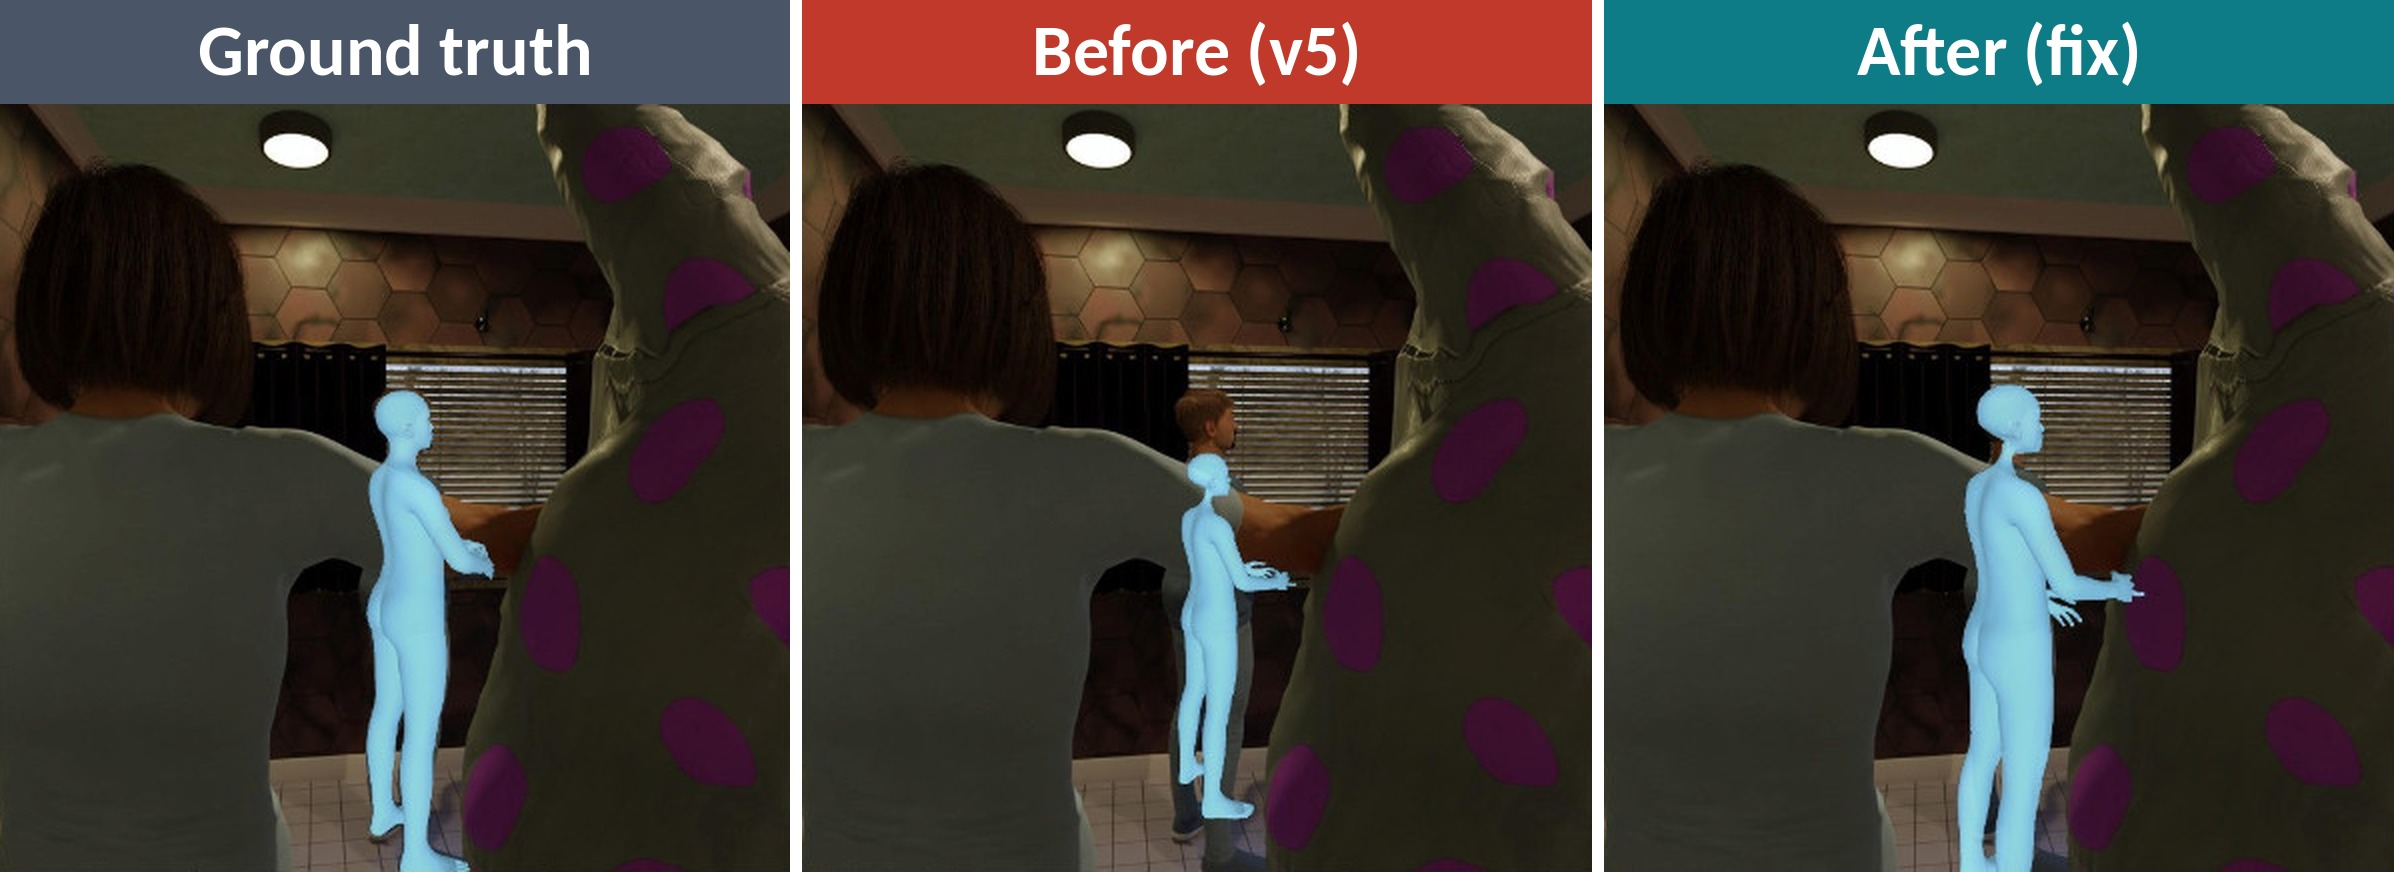
\includegraphics[width=0.9\linewidth]{depth_before_after_579860}
\caption[Holdout image 579860 at the predicted depth: ground truth, Base, depth pilot]{Holdout image 579860
rendered at each model's own predicted depth: ground truth, Base, and the depth pilot (head-joint targets, depth
weight $\times$5, 10 epochs, AnnyOne only). Before the fix the ground-truth head shows above a shrunken body placed
too far away. Synthetic image; one case, not a typical one. Companion of Figure~\ref{fig:depth-579862}.}
\label{fig:depth-579860}
\end{figure}

% F23: exp6 compare panels on the holdout (Base without and with the bone correction, no training; job in Appendix A).
\begin{figure}[tbp]
\centering
\includegraphics[width=0.49\linewidth]{exp6_compare_579864}\hfill
\includegraphics[width=0.49\linewidth]{exp6_compare_579866}
\caption[Two more holdout pairs: Base without and with the bone correction]{Holdout images 579864 (left) and 579866
(right): Base as trained next to the same checkpoint with the bone correction applied at the output, no training
(Section~\ref{sec:diag-neck}). Synthetic images, bodies at the model's own predicted depth, so the depth bug still
draws them too small; necks judged by eye. Companions of Figure~\ref{fig:diag-neck-base}.}
\label{fig:exp6-compare}
\end{figure}

% F9 office pair (plan section 3). Source docs/figures/neck_before_after_3dpw_bar_office.jpg.
\begin{figure}[tbp]
\centering
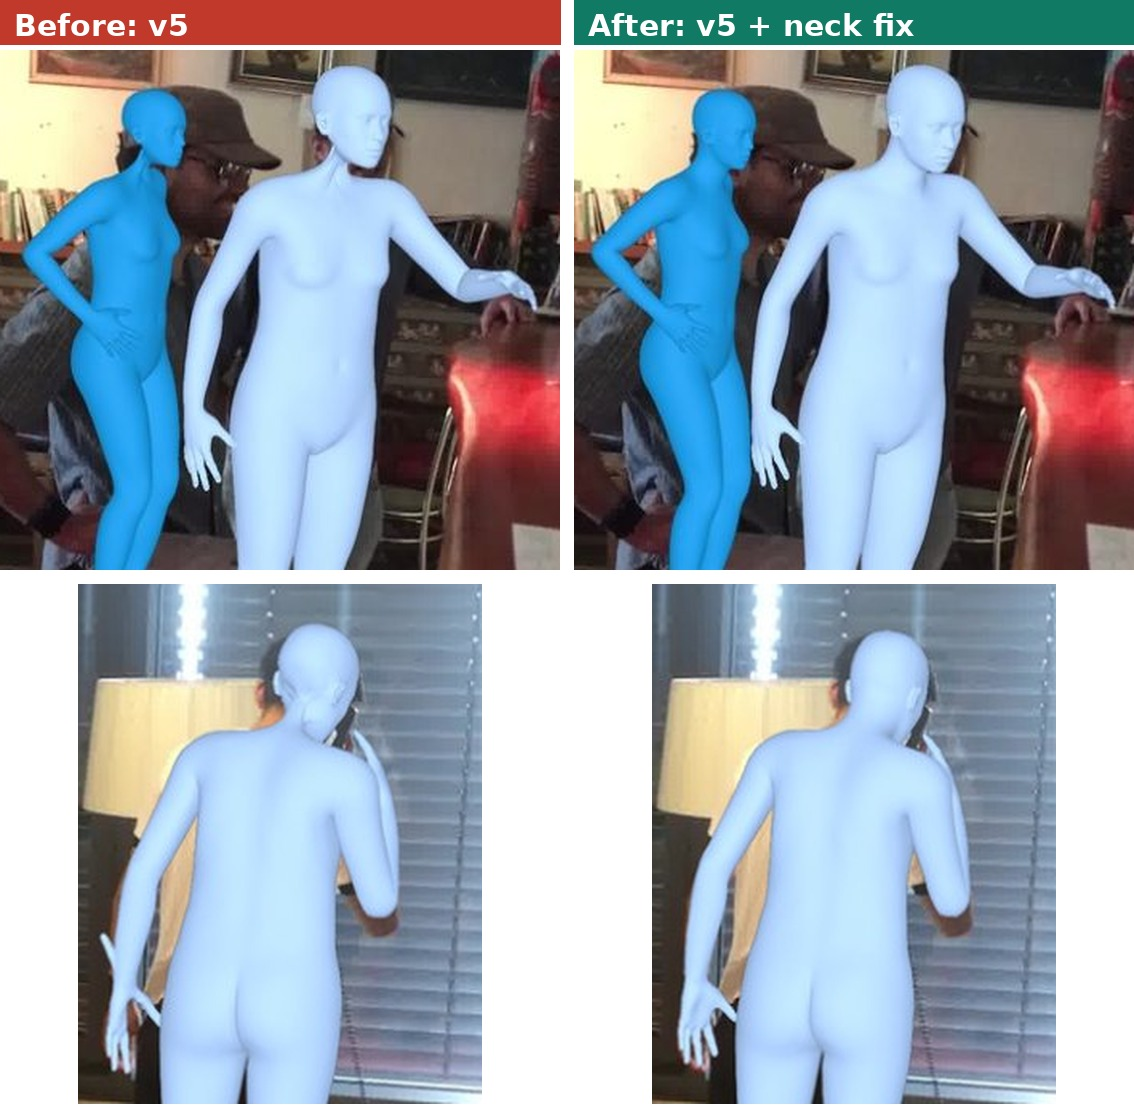
\includegraphics[width=0.9\linewidth]{neck_before_after_3dpw_bar_office}
\caption[Two 3DPW test frames: Base against the neck pilot]{Real 3DPW test frames \texttt{downtown\_bar\_00} 701
(top) and \texttt{office\_phoneCall\_00} 440 (bottom): Base next to the neck pilot (the bone correction and a 2-epoch
fine-tune); necks ringed. Bodies placed from the detector box, fingers at rest pose; judged by eye, no metric. The two
columns differ by the correction and by the fine-tune.}
\label{fig:neck-3dpw-office}
\end{figure}

% F10, the other four 3DPW test frames of the demo (photo | Base | photo | Final, labels baked into the image).
\begin{figure}[tbp]
\centering
\begin{subfigure}{0.495\linewidth}\centering
  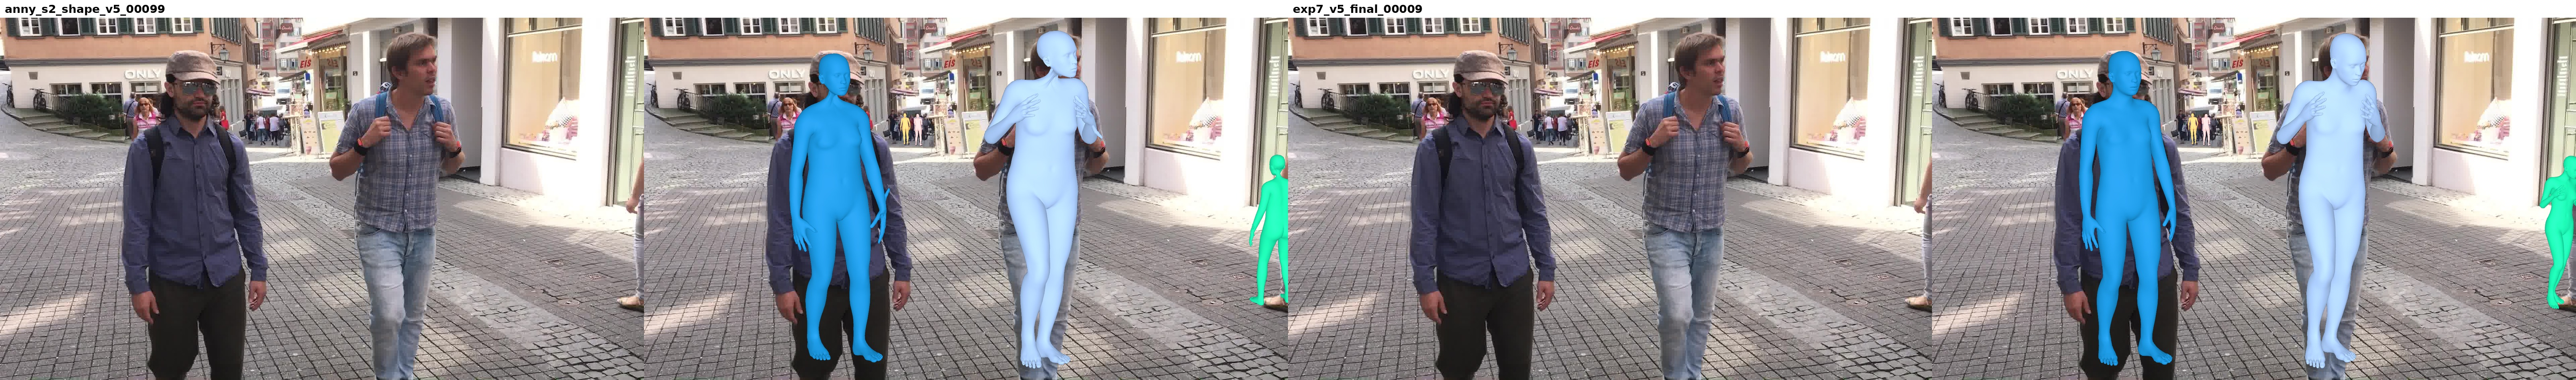
\includegraphics[width=\linewidth]{F10_3dpw_walking_v5_vs_final}\caption{\texttt{downtown\_walking}}\end{subfigure}\hfill
\begin{subfigure}{0.495\linewidth}\centering
  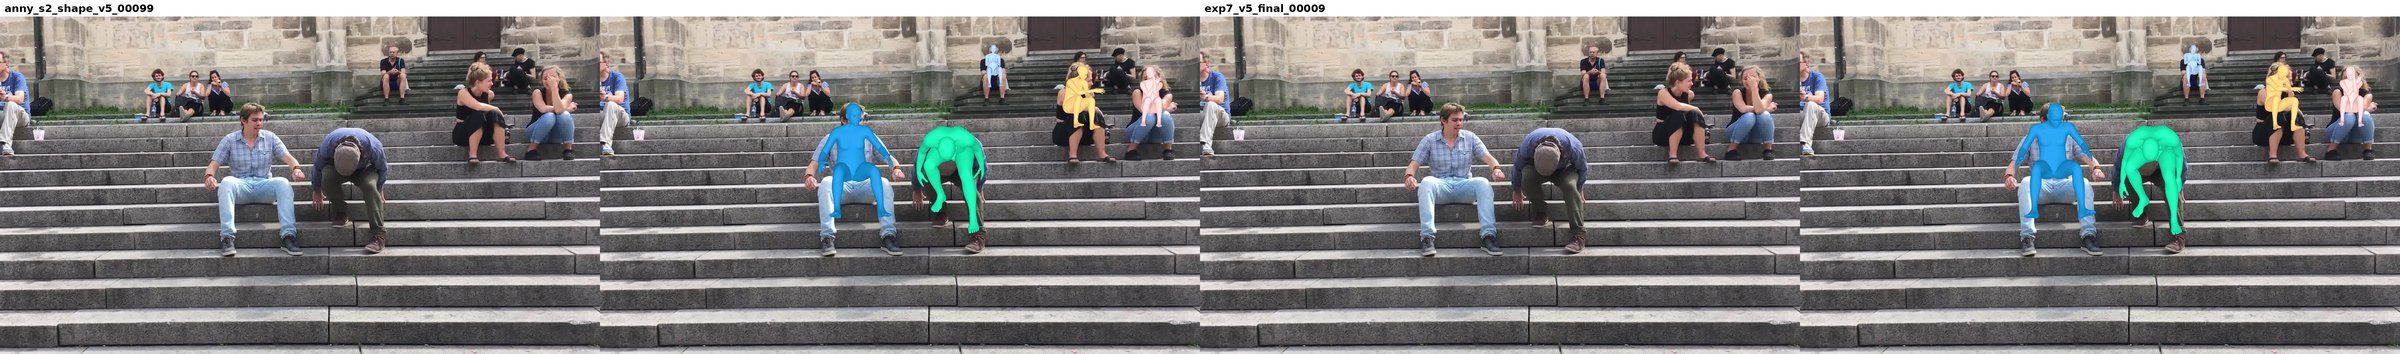
\includegraphics[width=\linewidth]{F10_3dpw_stairs_v5_vs_final}\caption{stairs}\end{subfigure}\\[4pt]
\begin{subfigure}{0.495\linewidth}\centering
  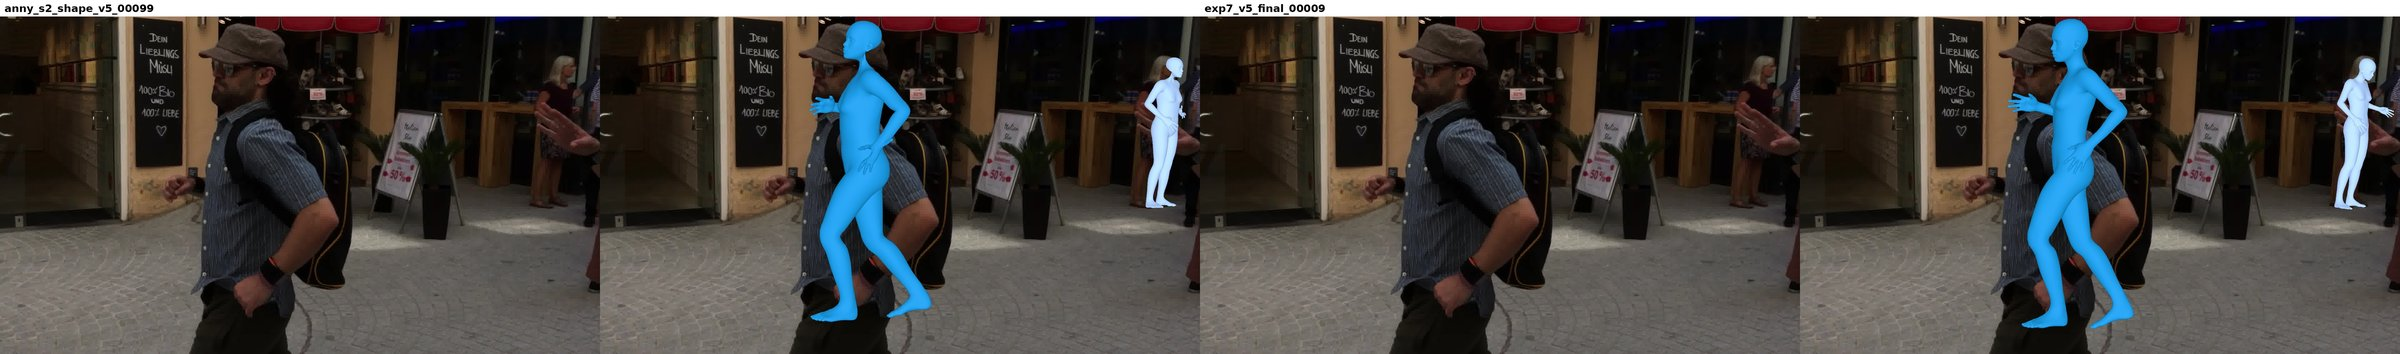
\includegraphics[width=\linewidth]{F10_3dpw_runforbus_v5_vs_final}\caption{\texttt{downtown\_runForBus}}\end{subfigure}\hfill
\begin{subfigure}{0.495\linewidth}\centering
  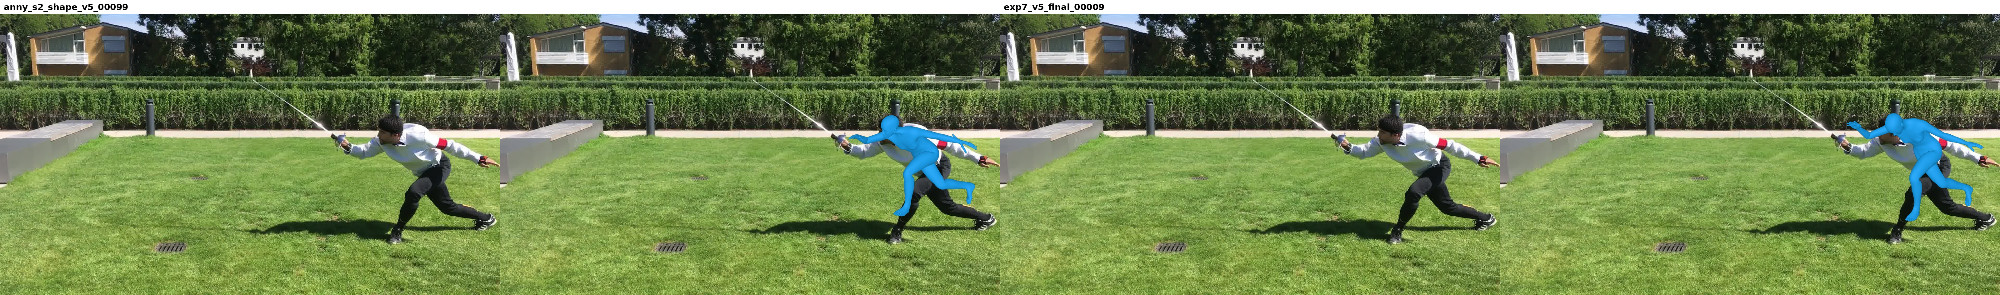
\includegraphics[width=\linewidth]{F10_3dpw_fencing_v5_vs_final}\caption{fencing}\end{subfigure}
\caption[Four more 3DPW test frames, Base against Final]{The other four 3DPW test frames of the demo, each shown as
photo and Base (left half), then photo and Final (right half; the labels in the image name the two checkpoints).
Bodies placed from the detector box, fingers at rest pose; judged by eye, no metric. The first four frames are in
Figure~\ref{fig:3dpw-overlays}.}
\label{fig:3dpw-overlays-more}
\end{figure}

% F10 photo montages (photo | Base | photo | Final, labels baked in).
\begin{figure}[tbp]
\centering
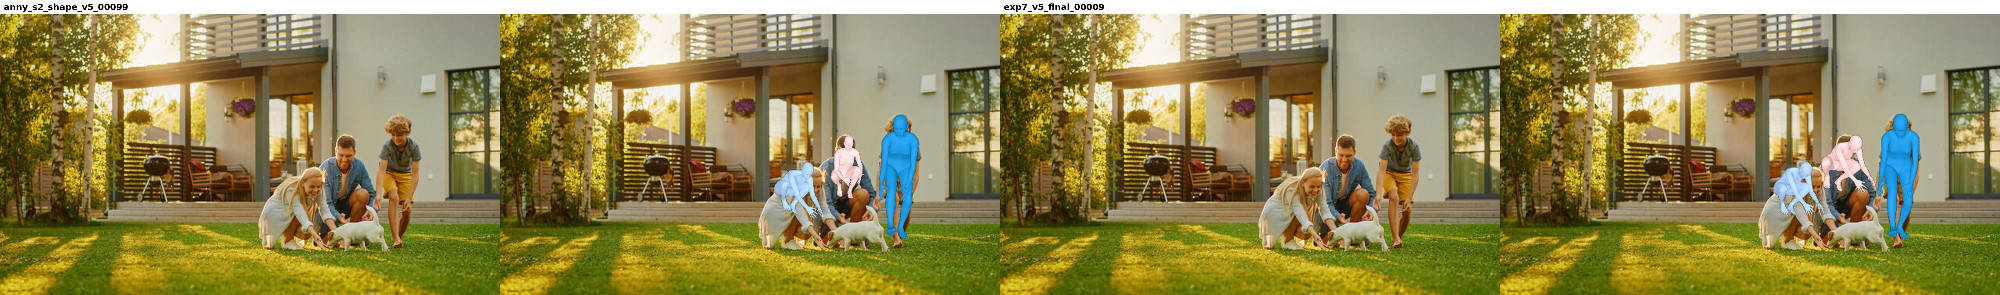
\includegraphics[width=\linewidth]{F10_photo_garden_v5_vs_final}\\[2pt]
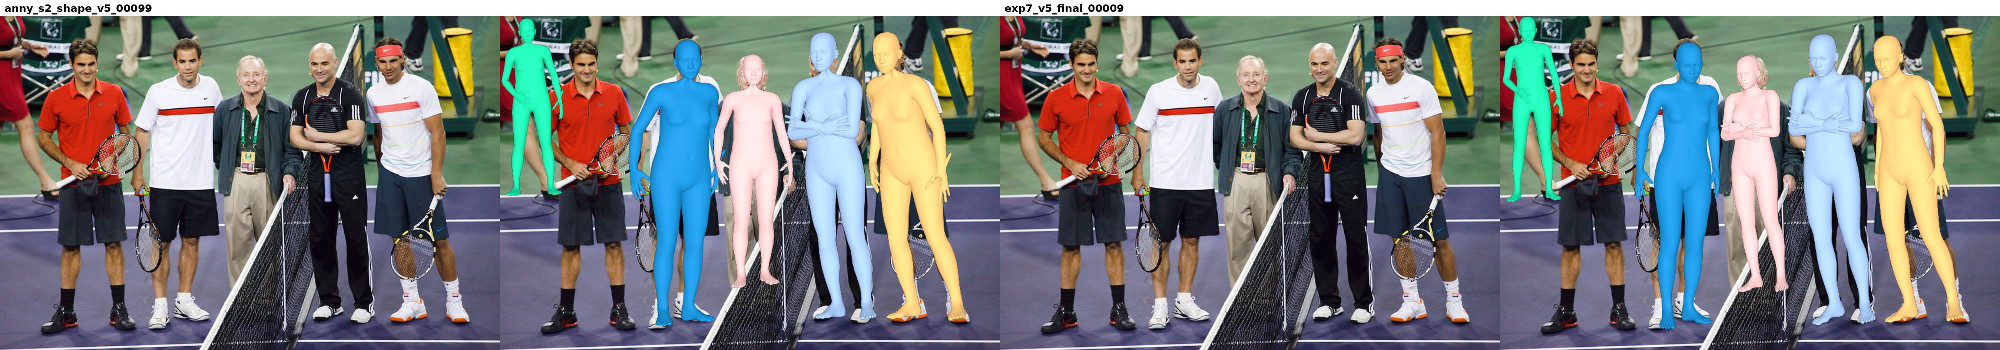
\includegraphics[width=\linewidth]{F10_photo_tennis_v5_vs_final}\\[2pt]
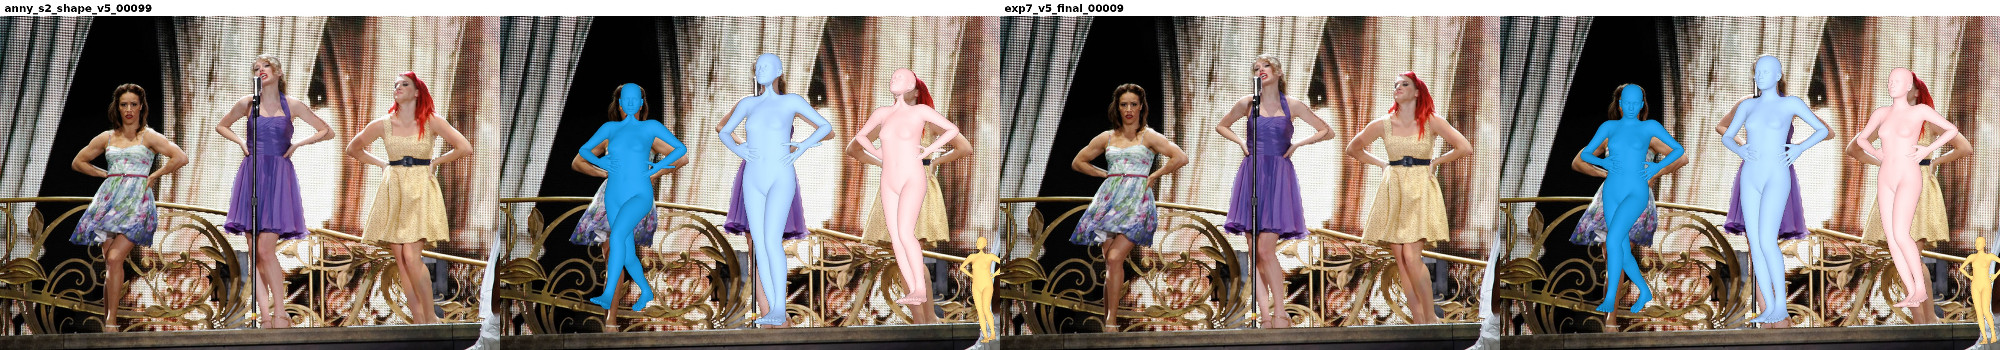
\includegraphics[width=\linewidth]{F10_photo_stage_v5_vs_final}\\[2pt]
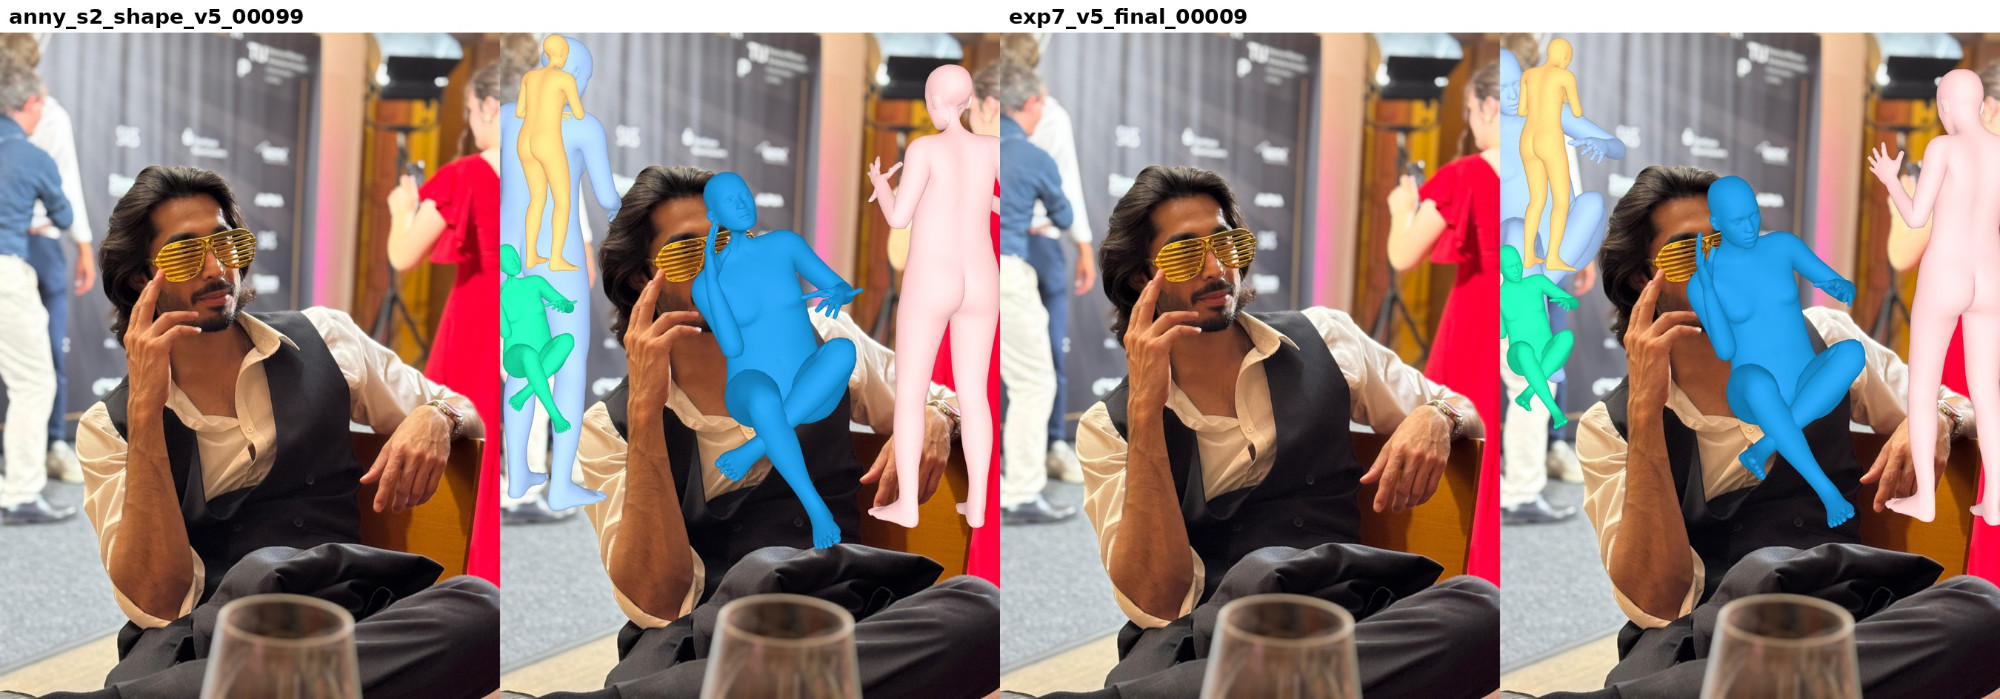
\includegraphics[width=\linewidth]{F10_photo_party_v5_vs_final}
\caption[Four real photos, Base against Final]{The four real photos of the demo (garden, tennis, stage, party), never
used in training, each shown as photo and Base, then photo and Final; bodies placed from the detector box, fingers at
rest pose; judged by eye, no metric. The tennis photo also appears in Figure~\ref{fig:real-photos}.}
\label{fig:photo-montages}
\end{figure}

% F11, all twelve montages (photo | Base | photo | Final, labels baked in; demo with --relax_hands 0). Chapter 6
% shows zoomed crops of party, guitar and bar only.
\begin{figure}[p]
\centering
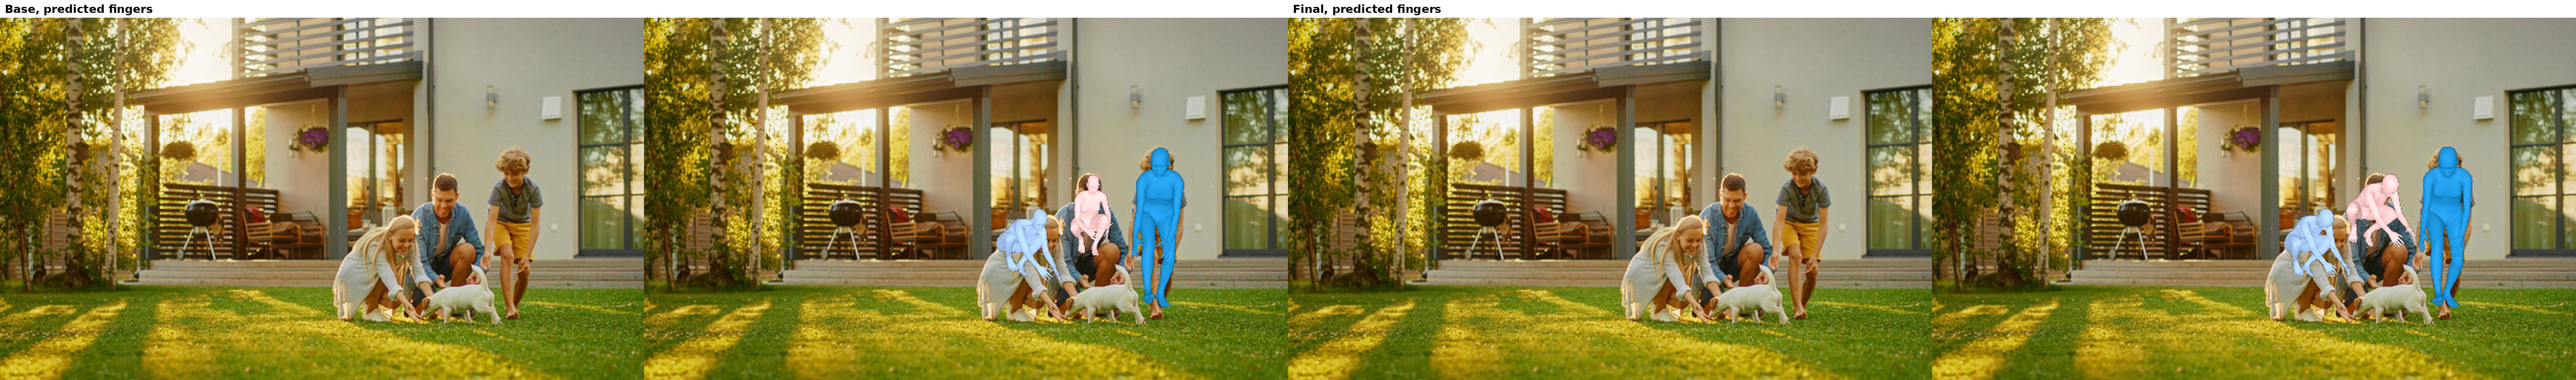
\includegraphics[width=0.82\linewidth]{F11_hands_photo_garden}\\[2pt]
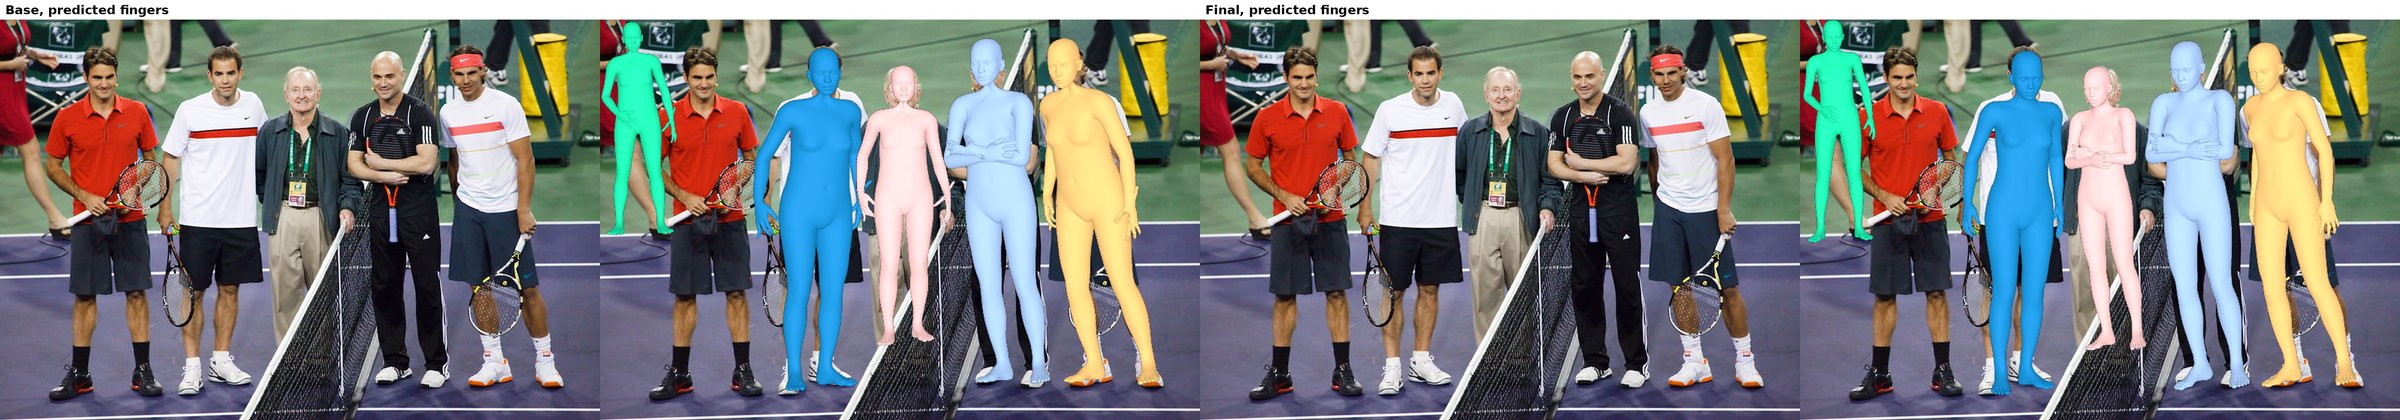
\includegraphics[width=0.82\linewidth]{F11_hands_photo_tennis}\\[2pt]
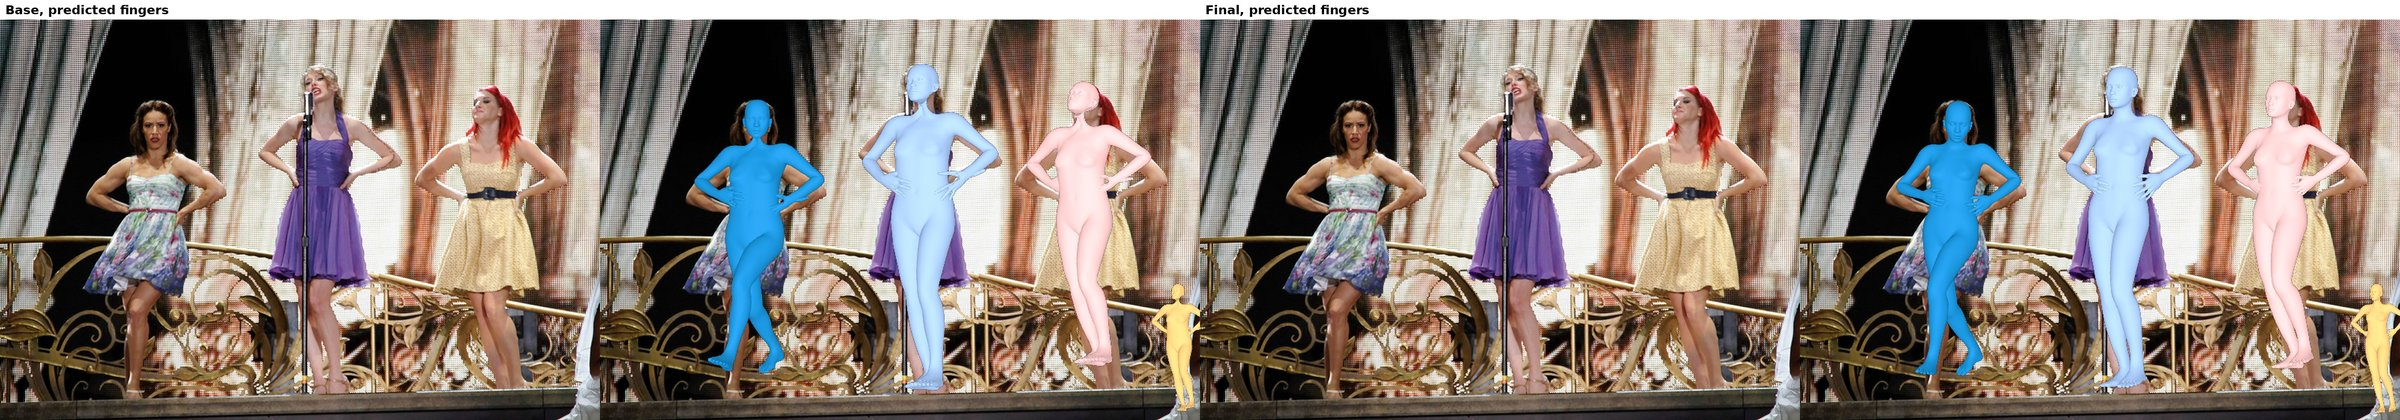
\includegraphics[width=0.82\linewidth]{F11_hands_photo_stage}\\[2pt]
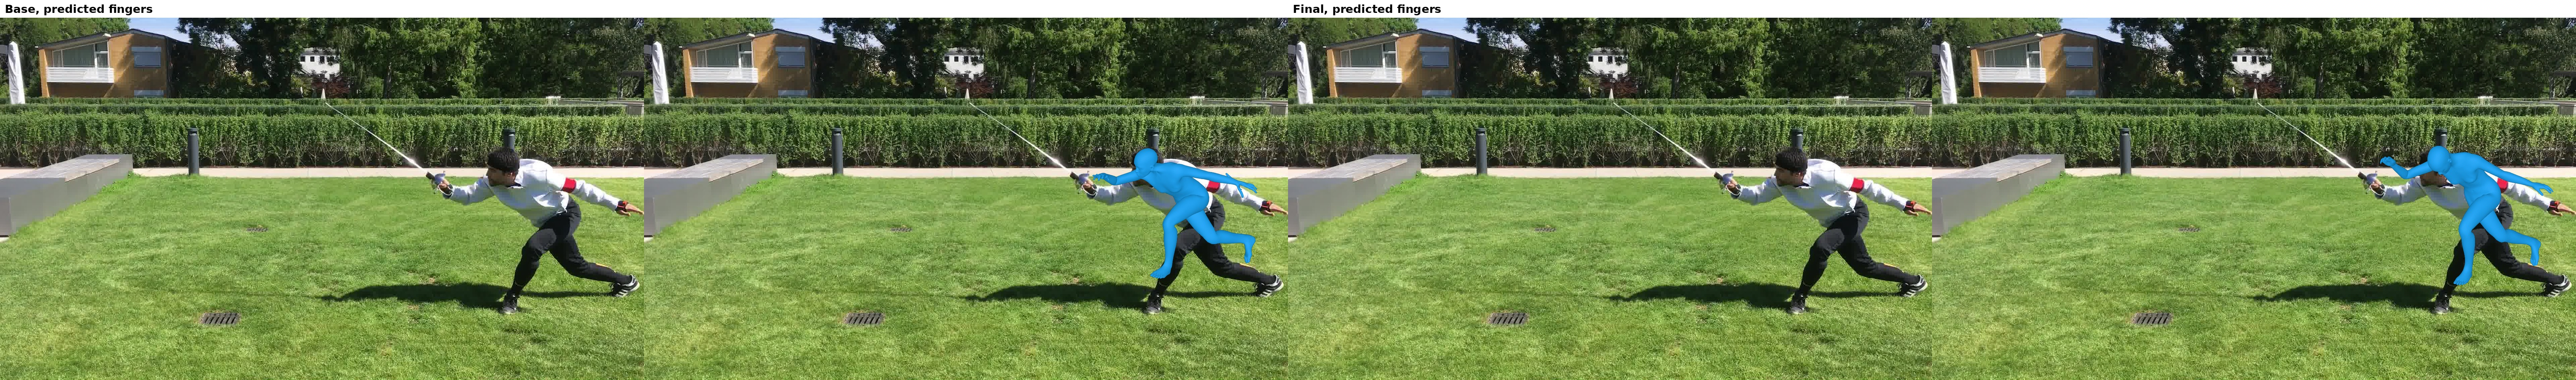
\includegraphics[width=0.82\linewidth]{F11_hands_3dpw_fencing}\\[2pt]
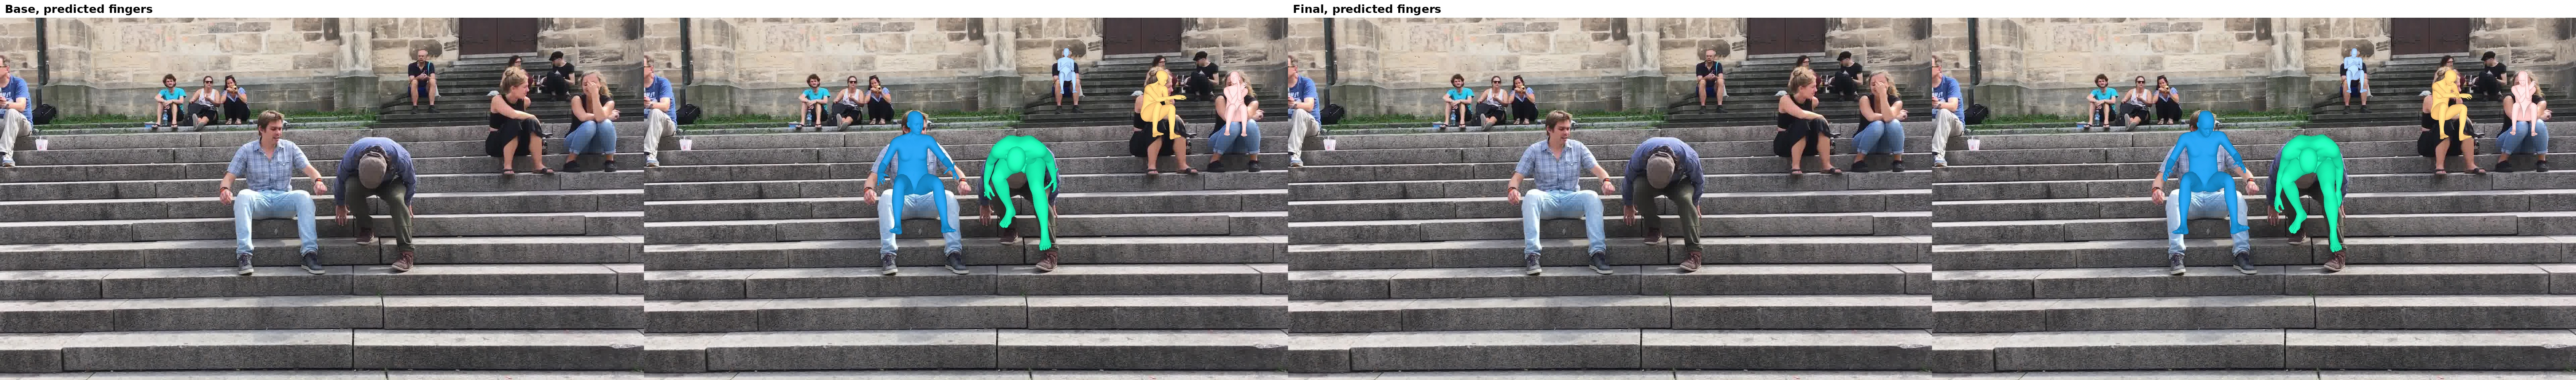
\includegraphics[width=0.82\linewidth]{F11_hands_3dpw_stairs}\\[2pt]
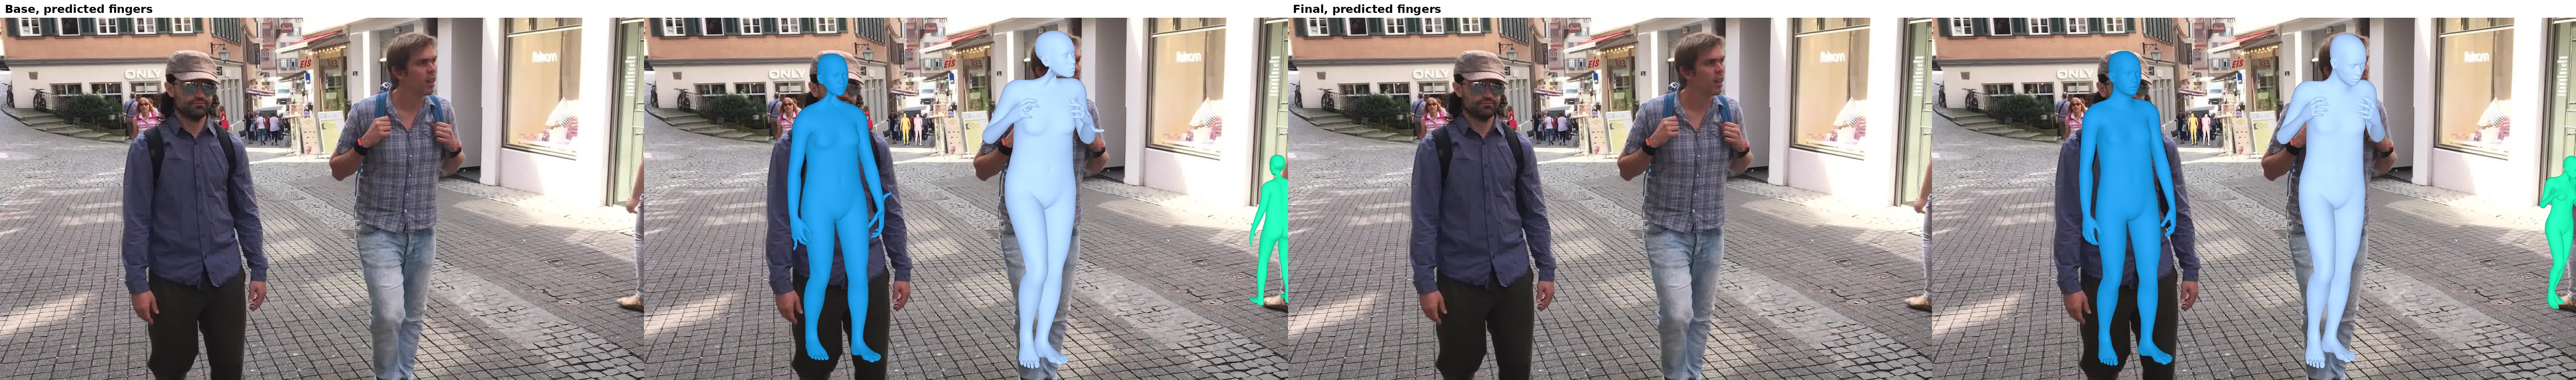
\includegraphics[width=0.82\linewidth]{F11_hands_3dpw_walking}\\[2pt]
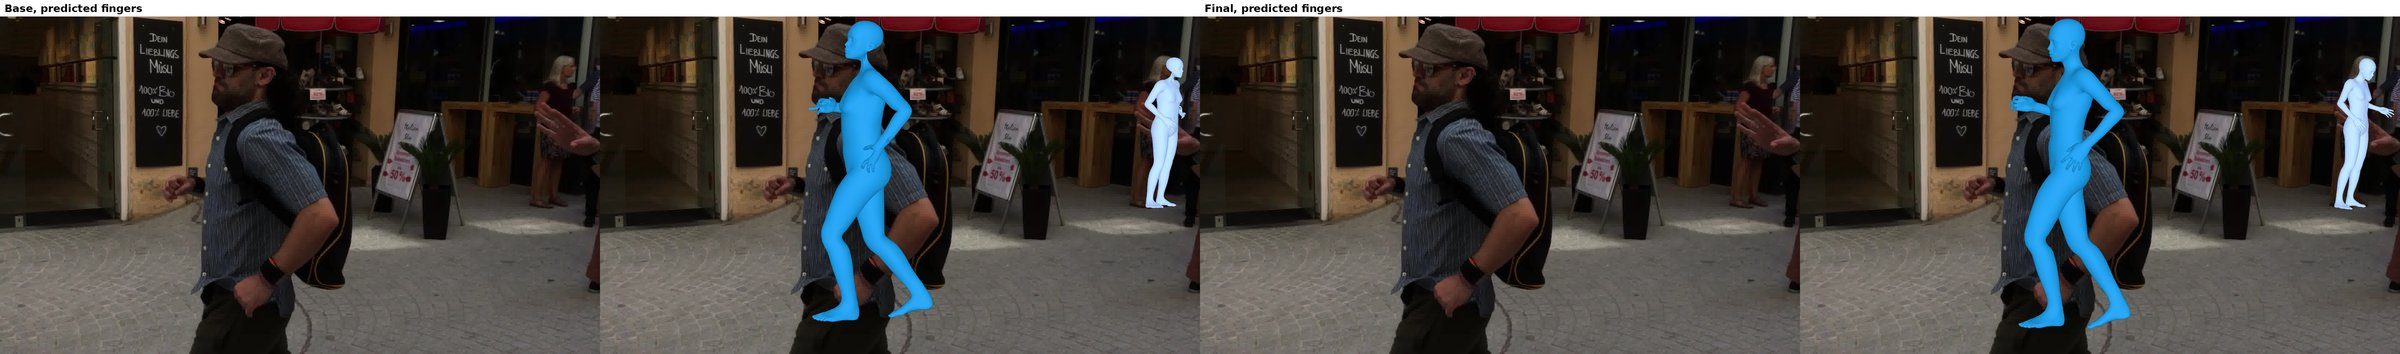
\includegraphics[width=0.82\linewidth]{F11_hands_3dpw_runforbus}\\[4pt]
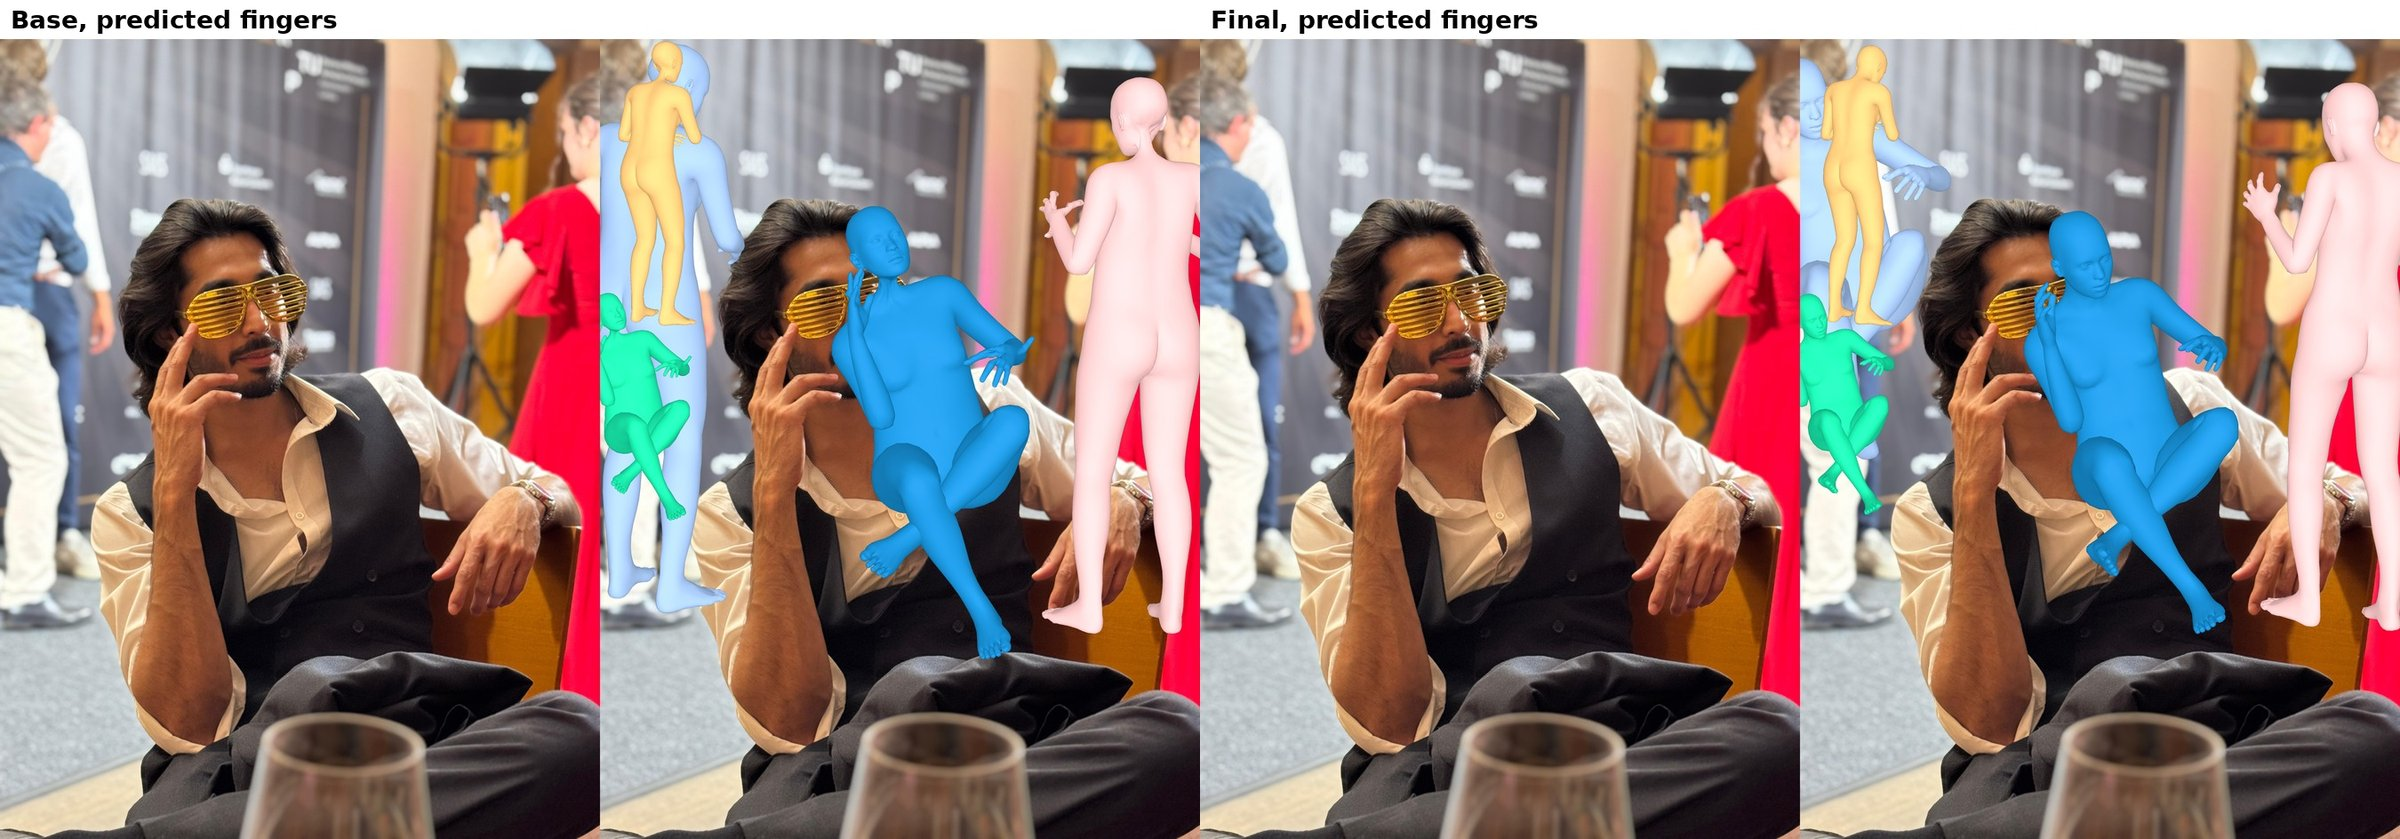
\includegraphics[width=0.385\linewidth]{F11_hands_photo_party}\hspace{2pt}%
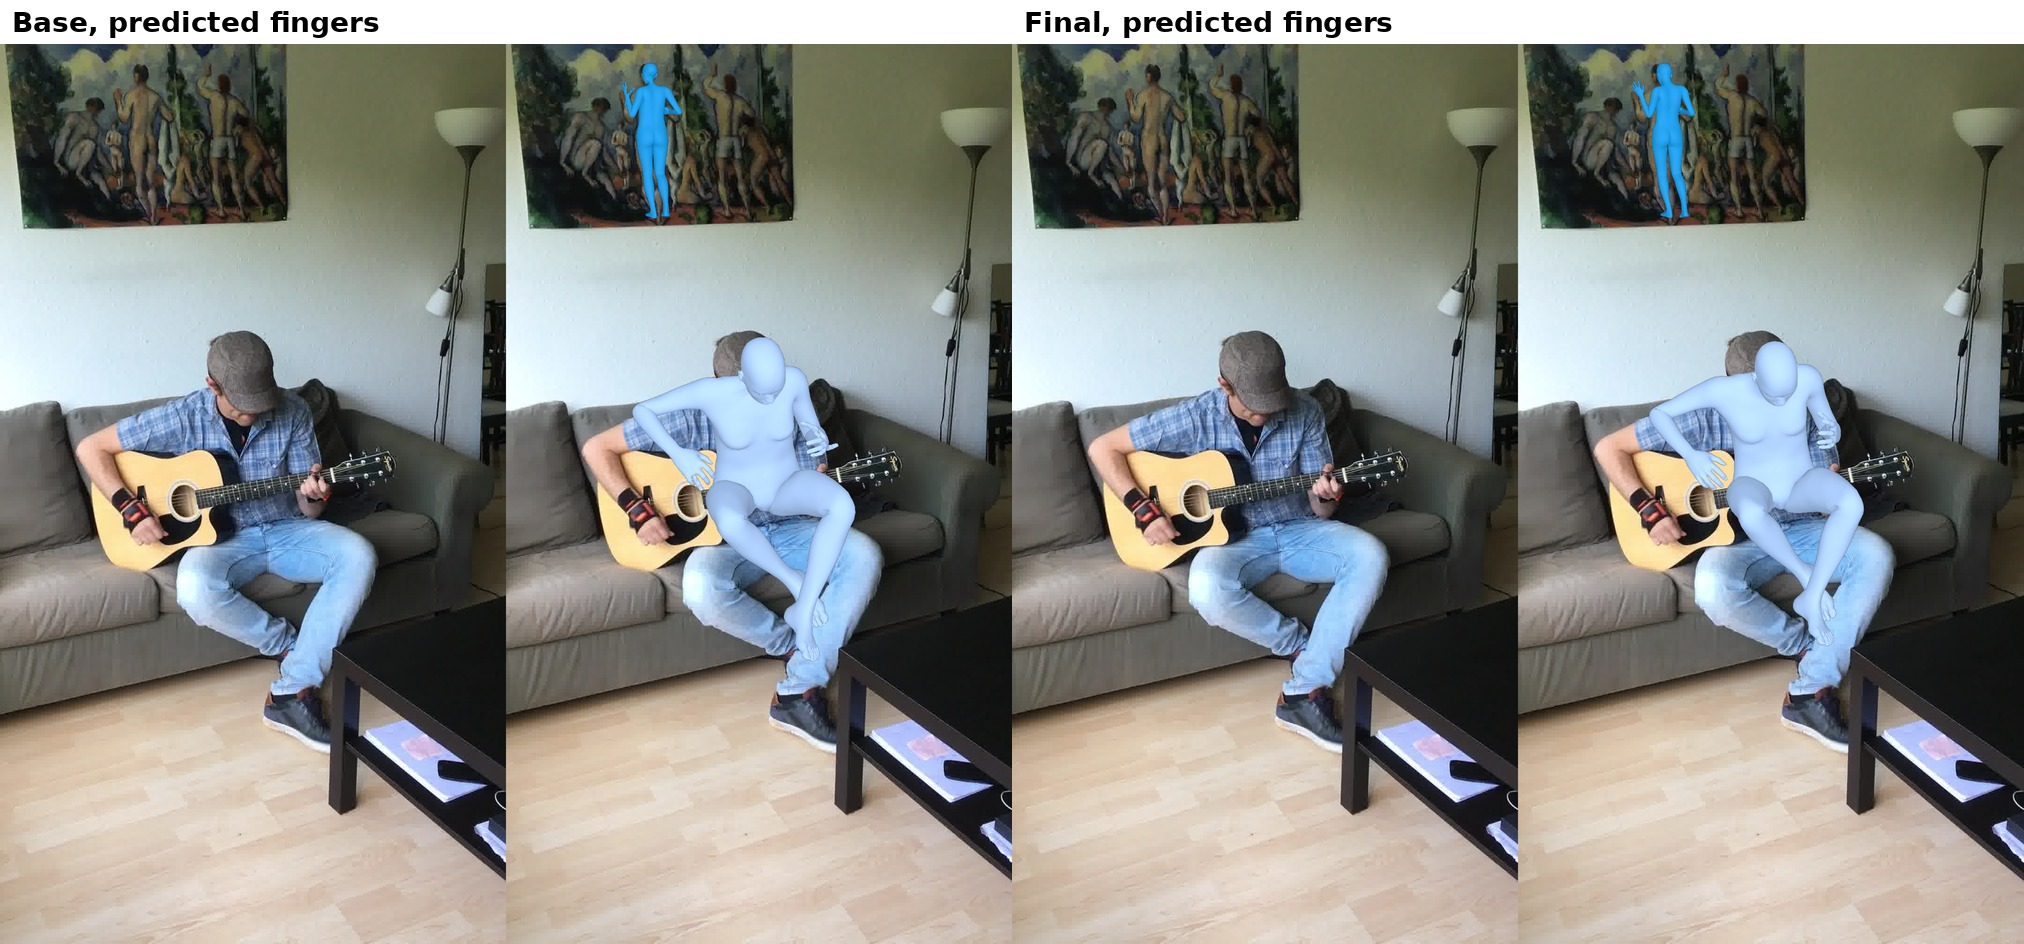
\includegraphics[width=0.288\linewidth]{F11_hands_3dpw_guitar}\hspace{2pt}%
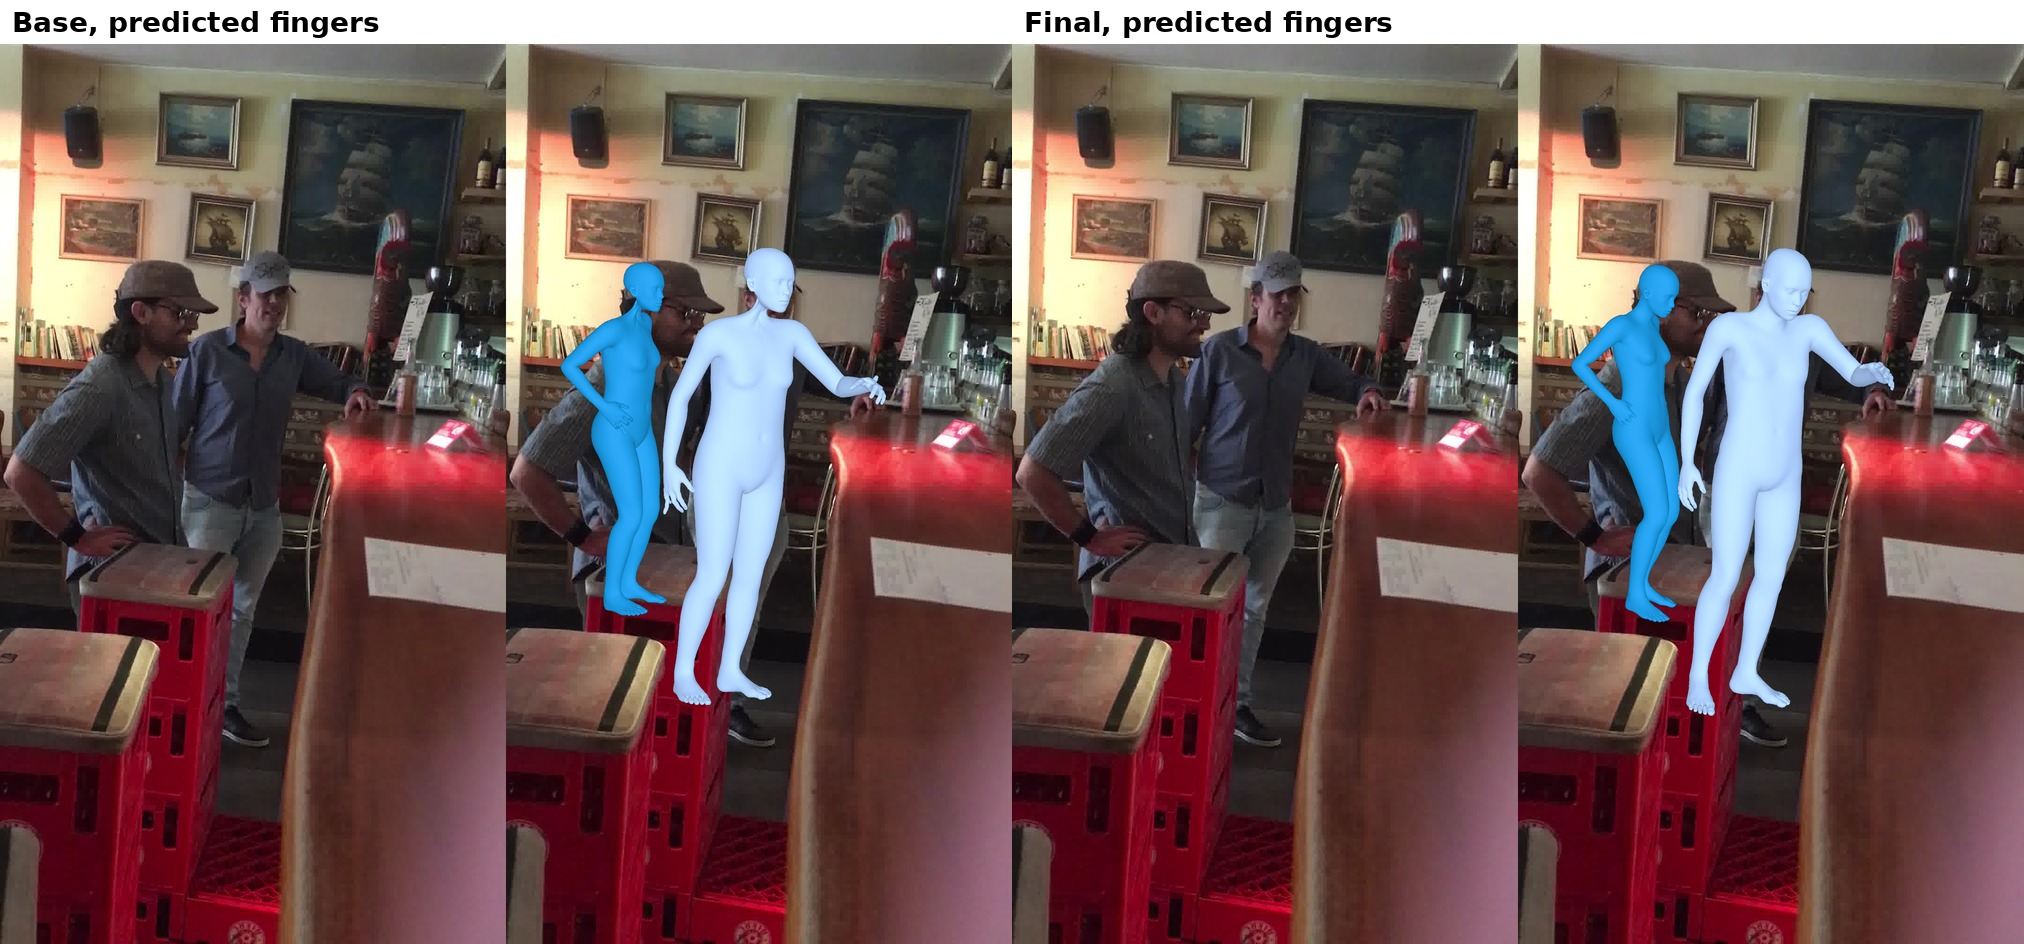
\includegraphics[width=0.288\linewidth]{F11_hands_3dpw_bar}\\[2pt]
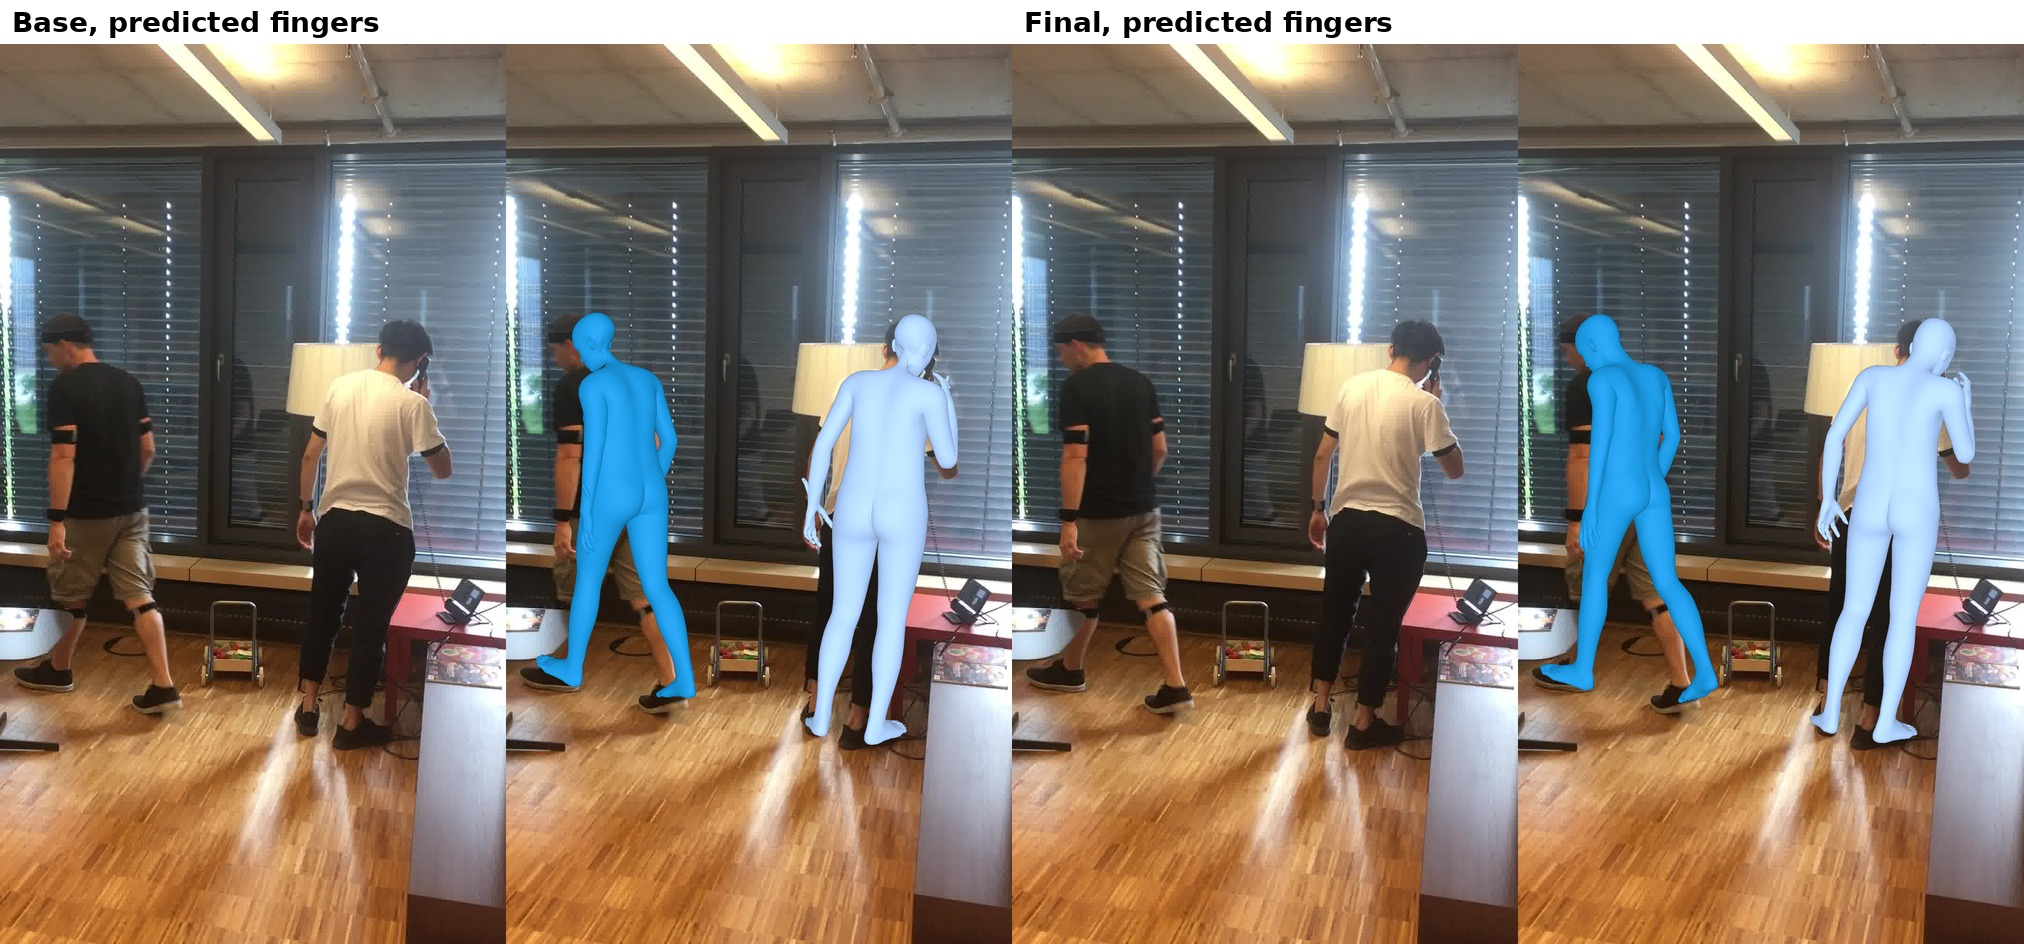
\includegraphics[width=0.288\linewidth]{F11_hands_3dpw_office}\hspace{2pt}%
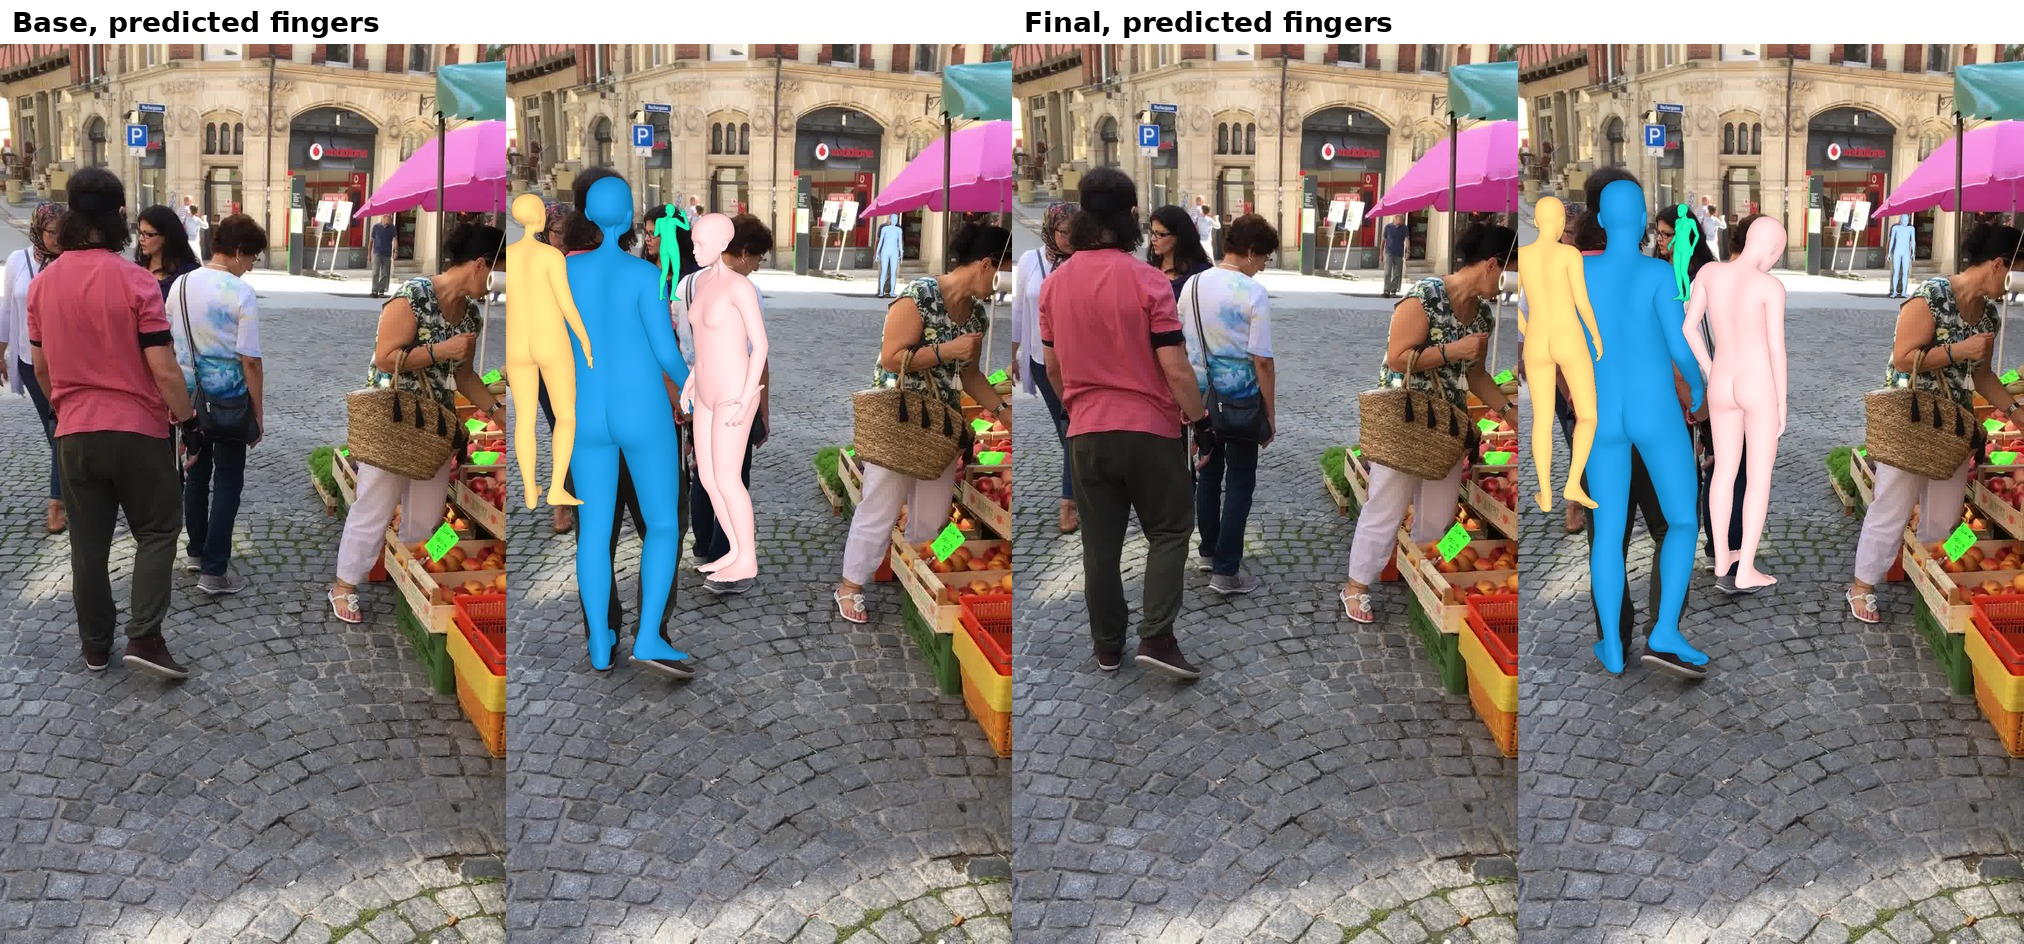
\includegraphics[width=0.288\linewidth]{F11_hands_3dpw_market}
\caption[All twelve demo images with predicted fingers, Base and Final]{All twelve demo images with predicted fingers
(not set to rest pose), each as photo and Base, then photo and Final (labels in the image). Top to bottom: the garden,
tennis and stage photos, the 3DPW test frames fencing, stairs, \texttt{downtown\_walking} and
\texttt{downtown\_runForBus}; then the party photo, guitar, \texttt{downtown\_bar}, \texttt{office\_phoneCall} and
the weekly market. Demo setting, bodies placed from the detector box; Base still has the flipped left index-finger
base (metacarpal1.L) and right ring-finger base, Final has the correction. In most of these images the hands are a
few pixels wide and cannot be judged; Figure~\ref{fig:fingers-demo} zooms on the three where they can. Judged by
eye; no metric.}
\label{fig:fingers-all}
\end{figure}

% F17, the nine rest-pose montages not shown in Chapter 6 (photo | Base | photo | Final | photo | Final-masked,
% labels baked in; demo with --rest_pose 1). Chapter 6 shows tennis, stage and downtown_bar.
\begin{figure}[p]
\centering
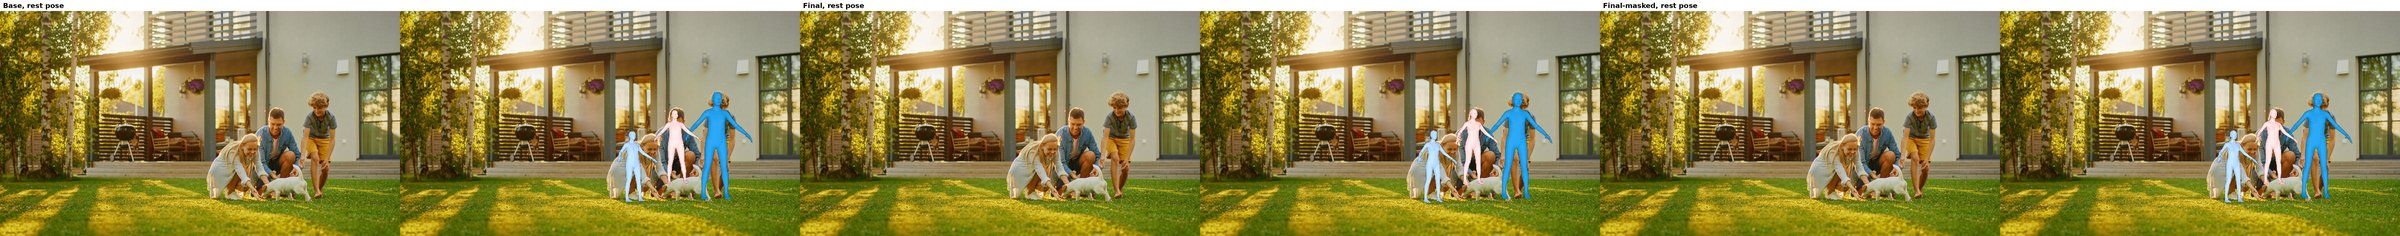
\includegraphics[width=0.9\linewidth]{F17_rest_photo_garden}\\[2pt]
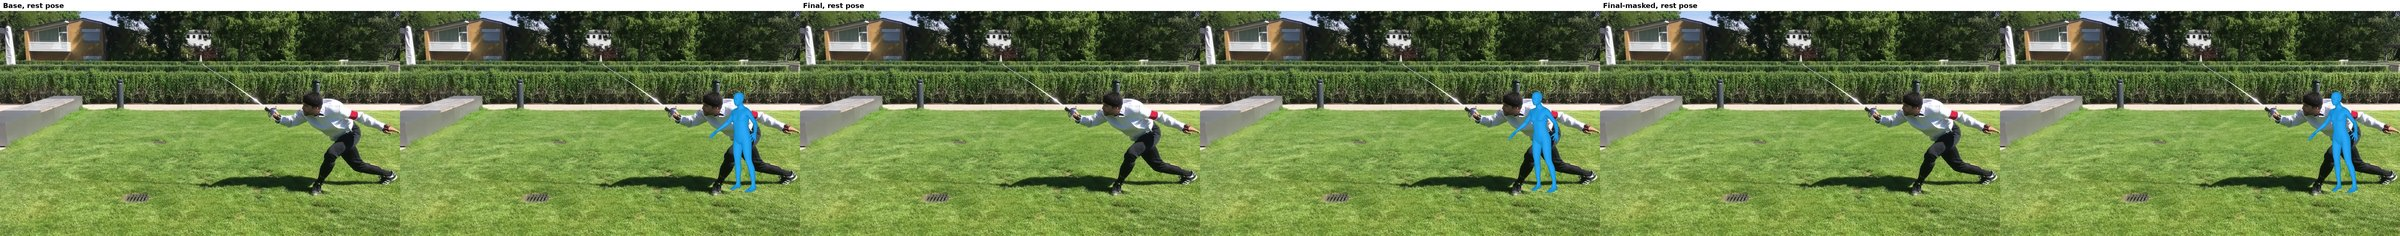
\includegraphics[width=0.9\linewidth]{F17_rest_3dpw_fencing}\\[2pt]
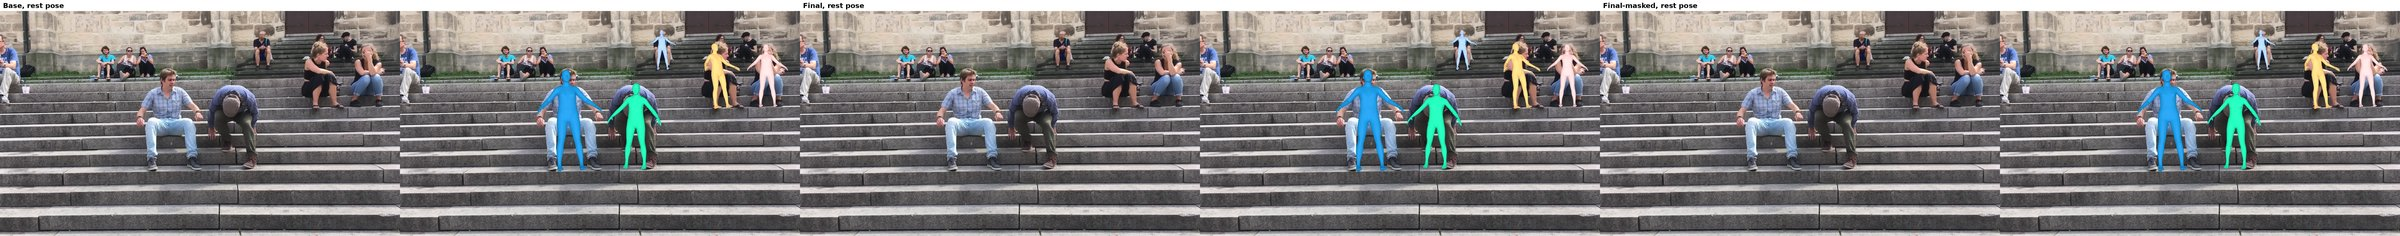
\includegraphics[width=0.9\linewidth]{F17_rest_3dpw_stairs}\\[2pt]
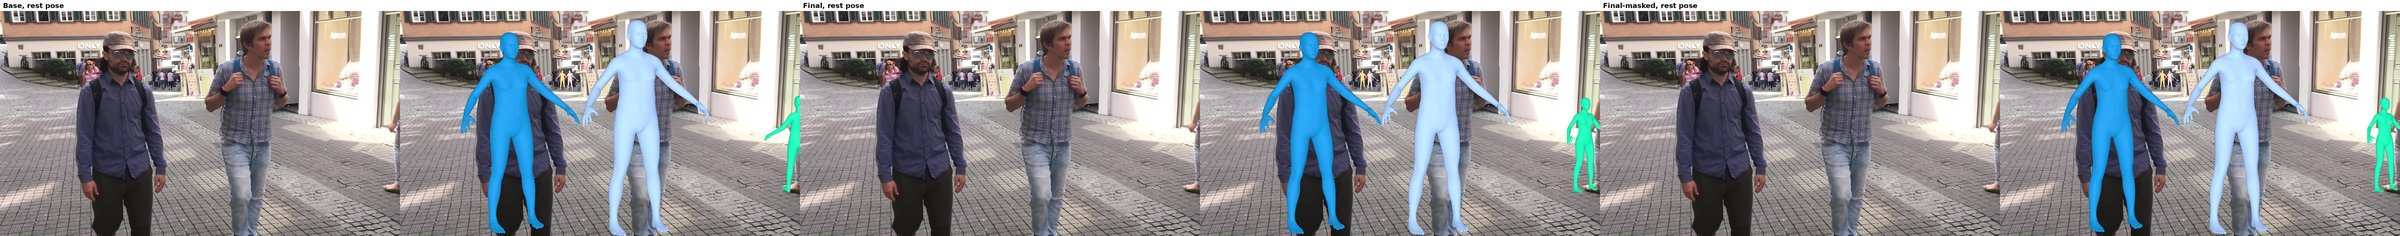
\includegraphics[width=0.9\linewidth]{F17_rest_3dpw_walking}\\[2pt]
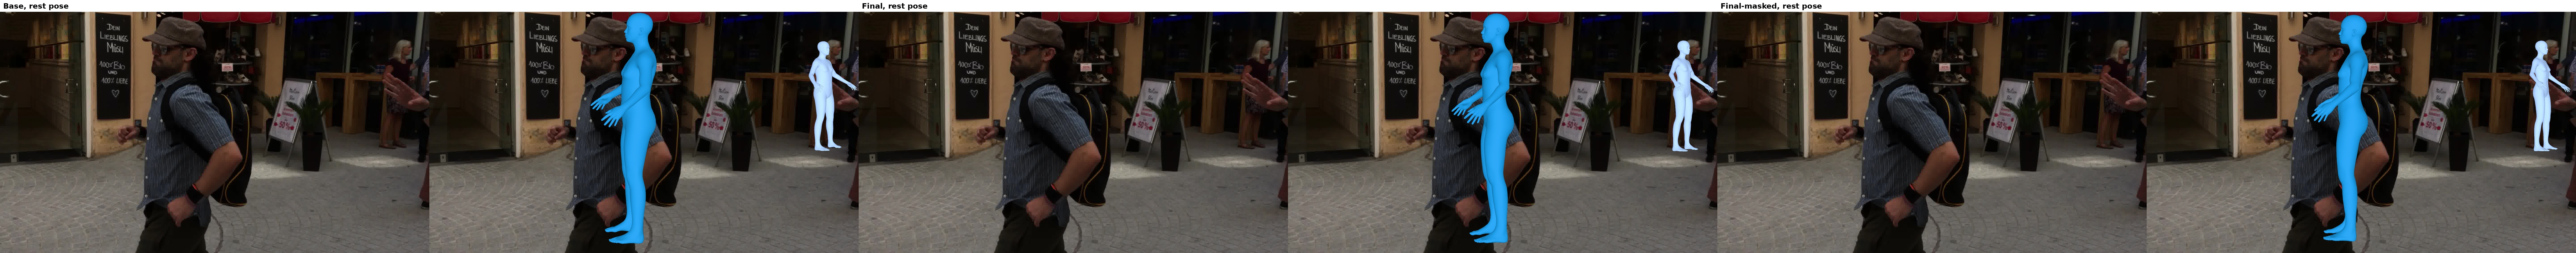
\includegraphics[width=0.9\linewidth]{F17_rest_3dpw_runforbus}\\[4pt]
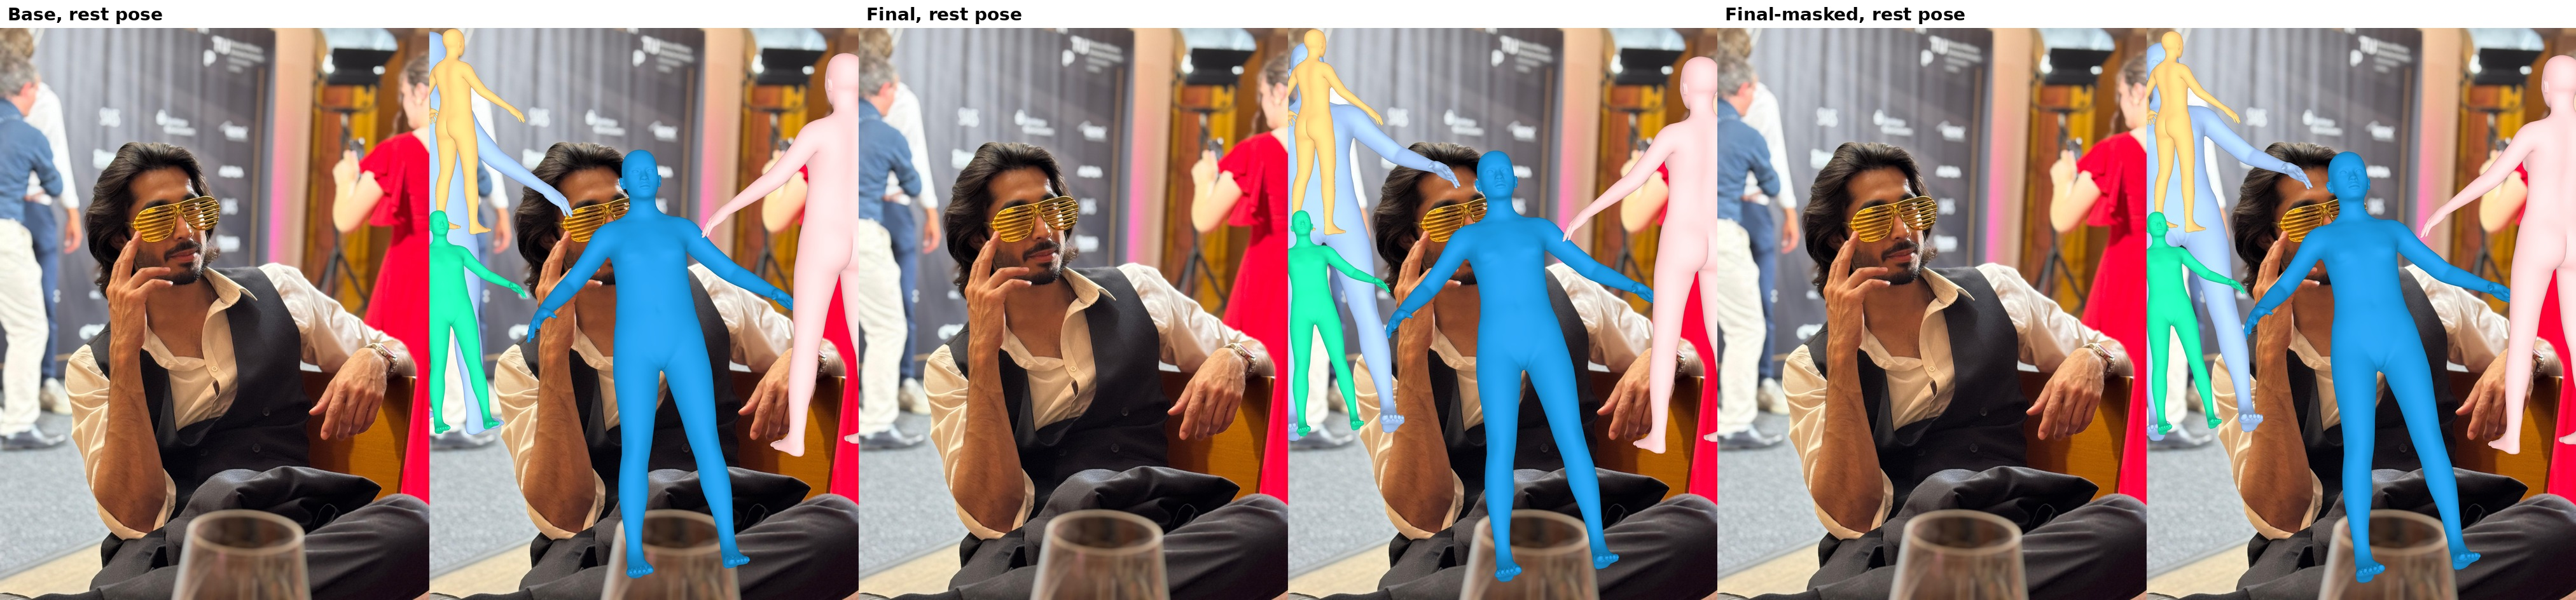
\includegraphics[width=0.495\linewidth]{F17_rest_photo_party}\hfill
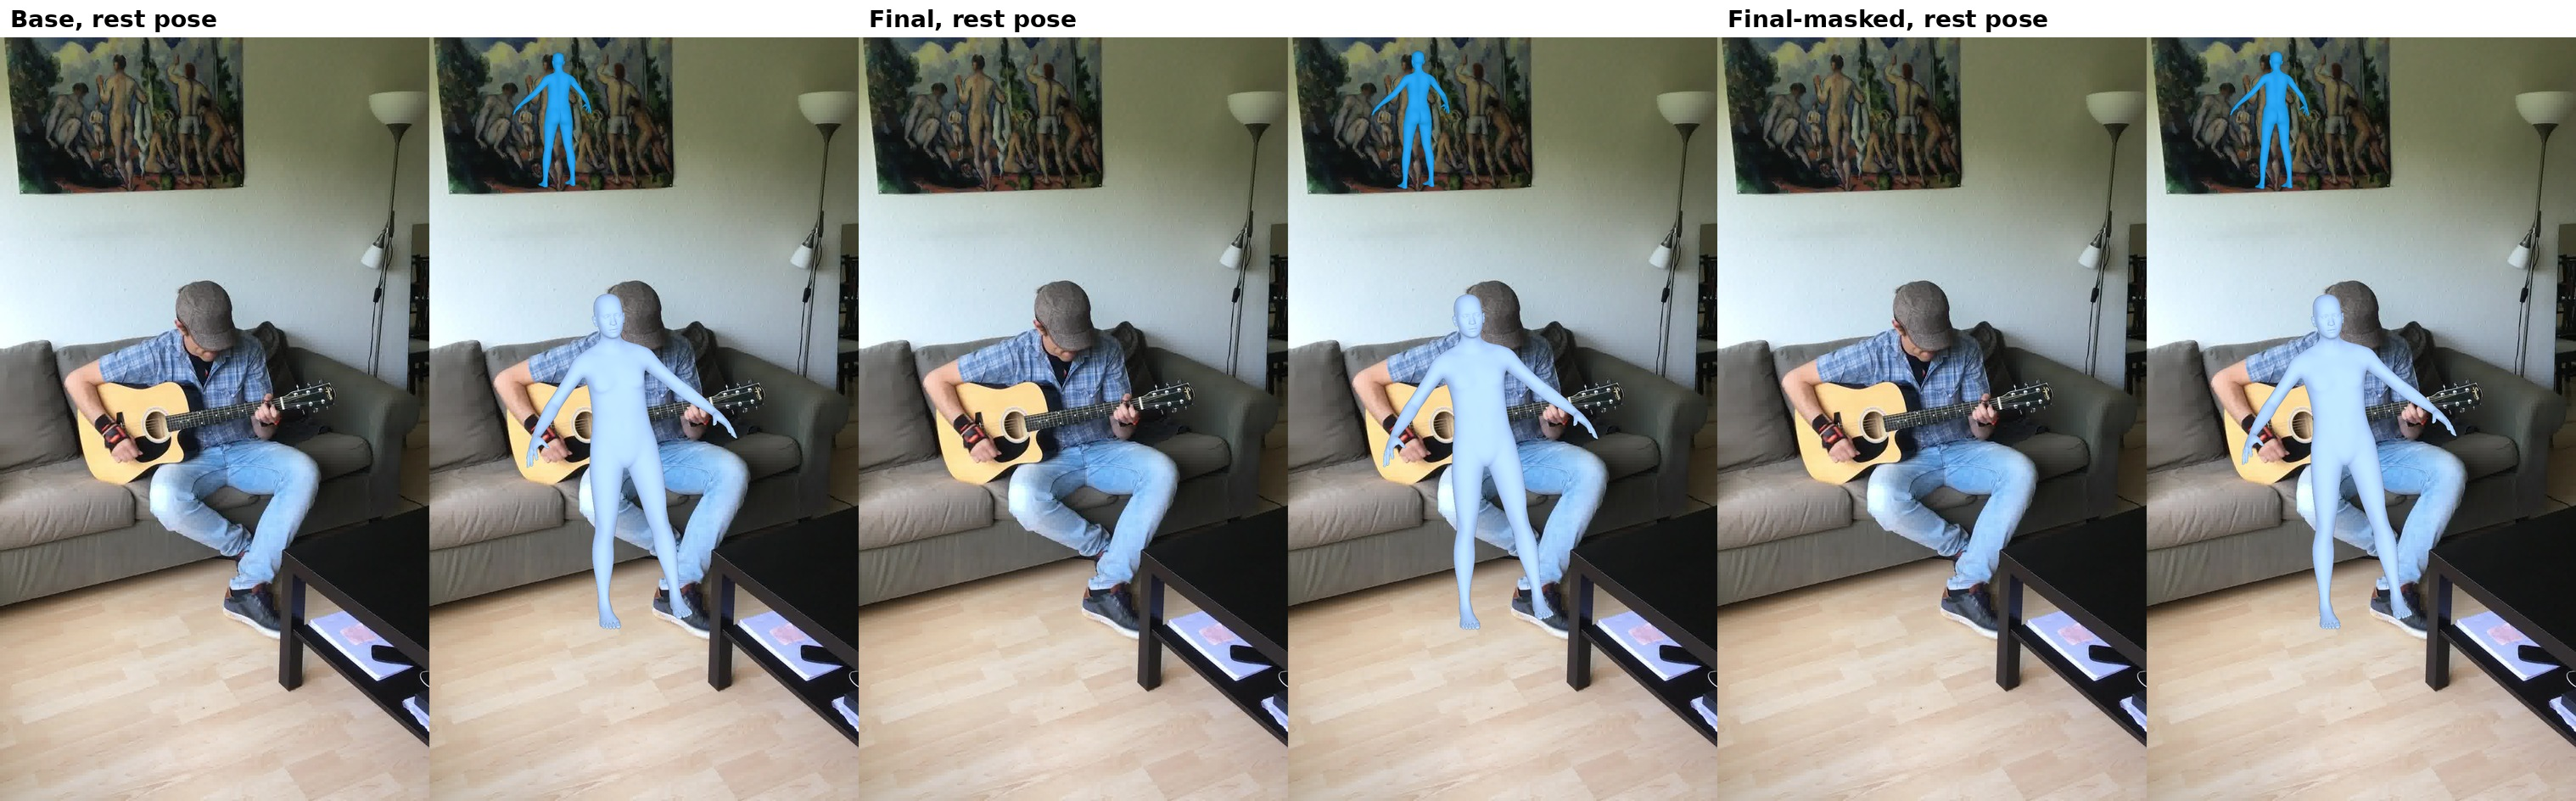
\includegraphics[width=0.495\linewidth]{F17_rest_3dpw_guitar}\\[2pt]
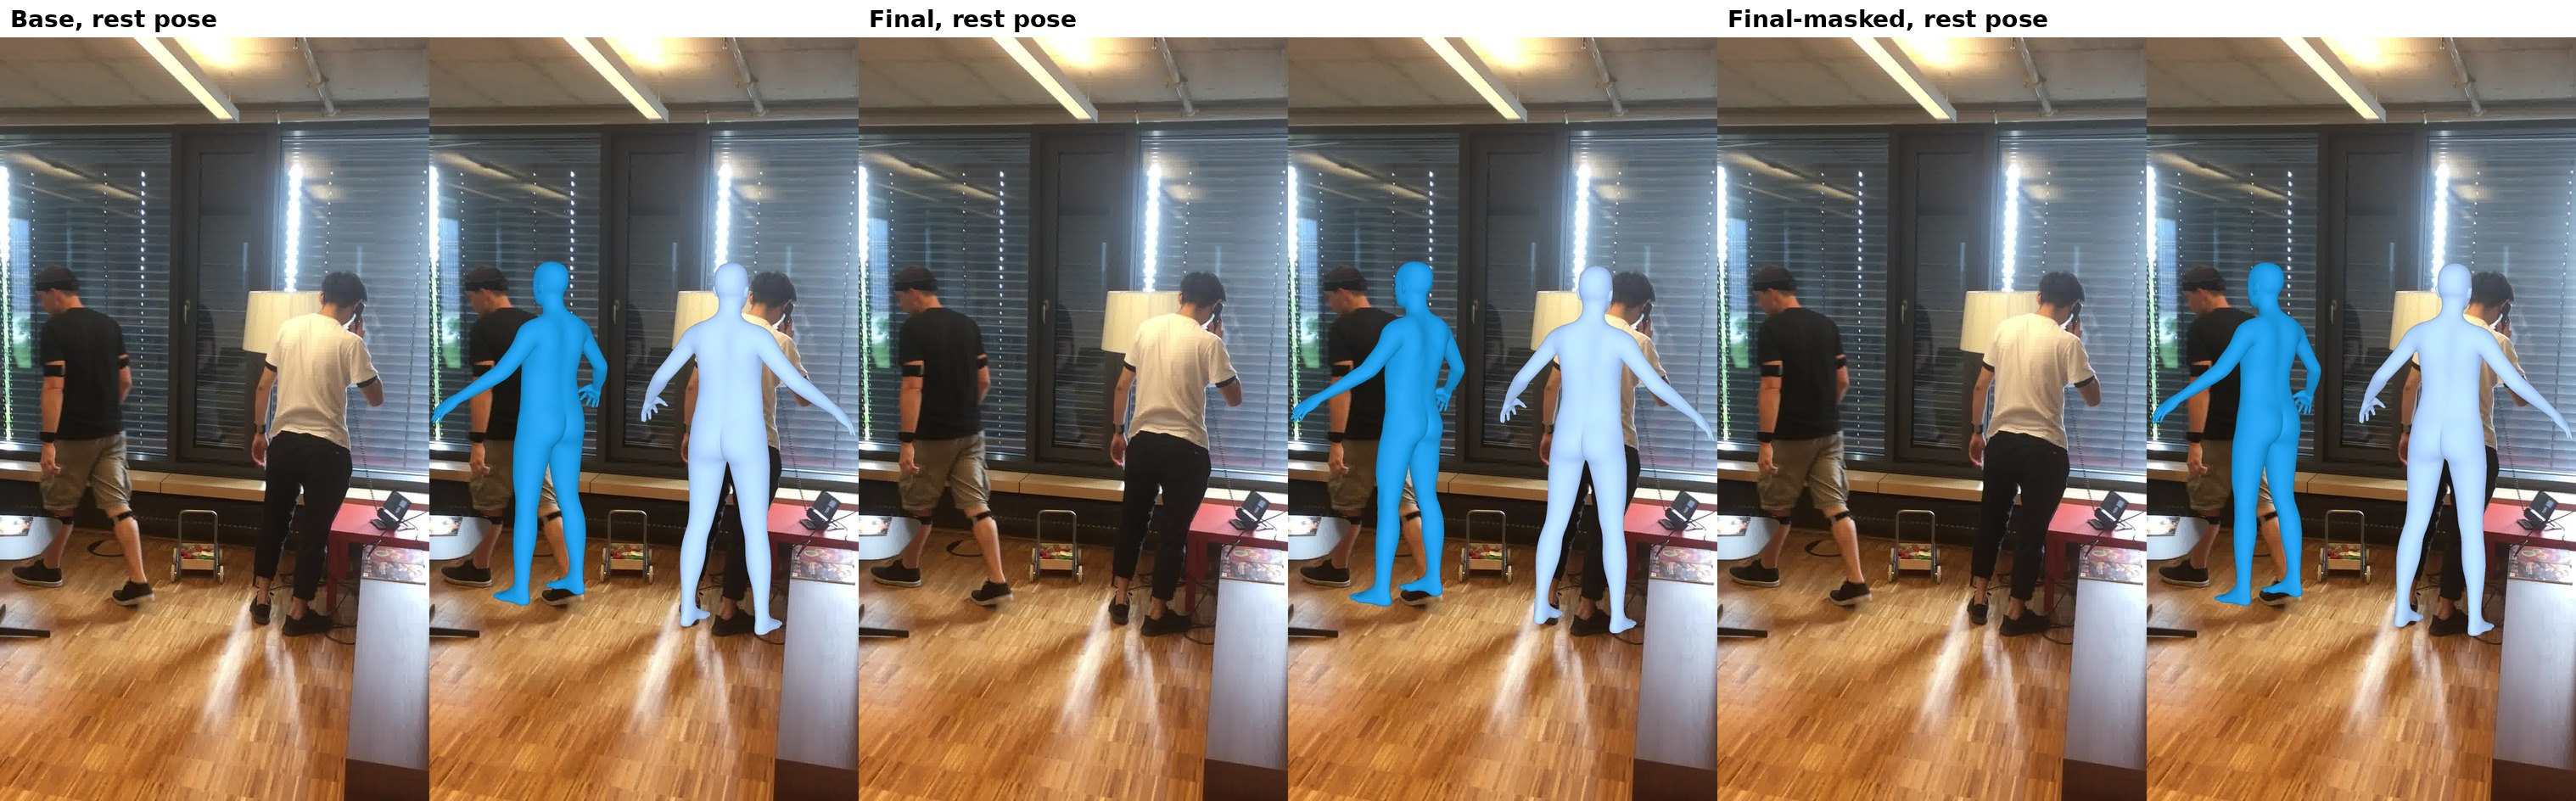
\includegraphics[width=0.495\linewidth]{F17_rest_3dpw_office}\hfill
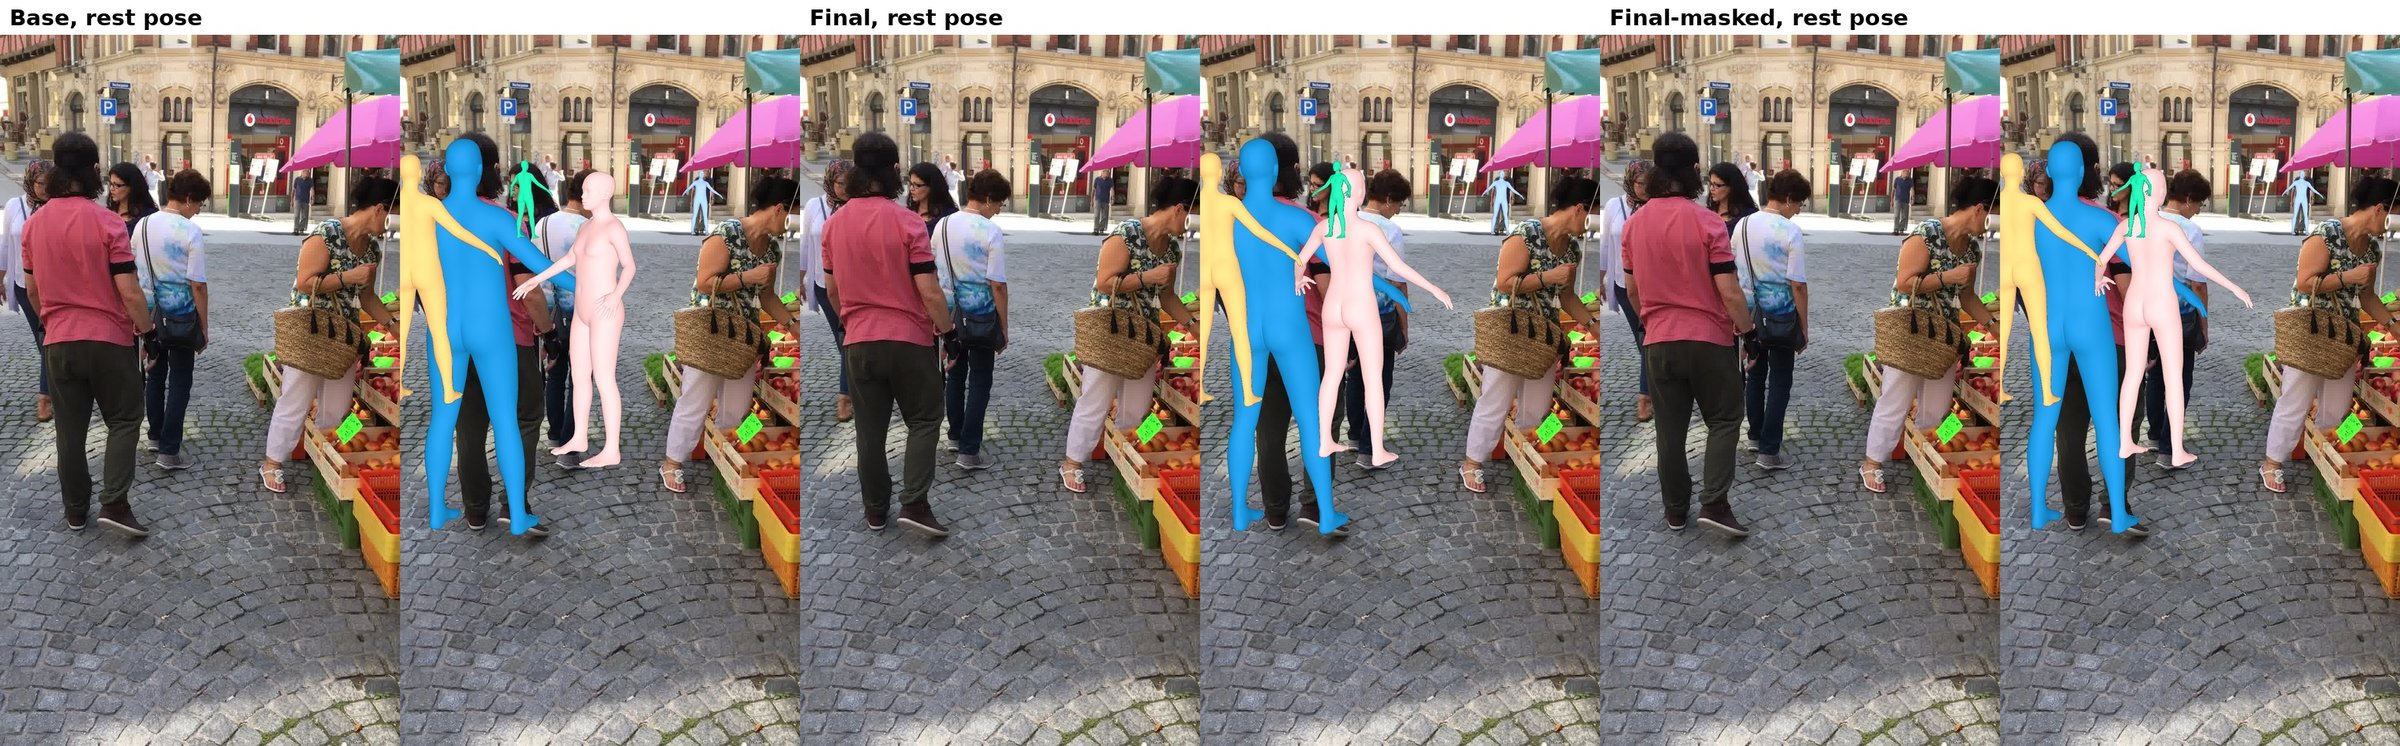
\includegraphics[width=0.495\linewidth]{F17_rest_3dpw_market}
\caption[Nine more rest-pose line-ups: Base, Final, Final-masked]{The other nine demo images in rest pose, each as
photo and Base, photo and Final, photo and Final-masked (labels in the image). Top to bottom: the garden photo, the
3DPW test frames fencing, stairs, \texttt{downtown\_walking} and \texttt{downtown\_runForBus}; then the party photo,
guitar, \texttt{office\_phoneCall} and the weekly market. Every detected person is in rest pose, so only body shape
differs. Demo setting, bodies placed from the detector box; at this size only gross differences of build can be
seen. Judged by eye; no metric. The other three images are in Figure~\ref{fig:rest-lineup}.}
\label{fig:rest-more}
\end{figure}

% appendix_e_pilots.tex -- Appendix E Pilot results in full.
% Skeleton from REWRITE_PLAN.md section 2. Writing rules: section 5 of the plan.
% "absorbs" = lines of draft_2026-10_original/main.tex (or the named draft file) whose content moves here.

\chapter{Pilot Results in Full}
\label{app:pilots}

% absorbs - (new)
% needs: H 3.1-3.4; exp1 full table (all arms, controls), exp2 children sampler, exp3 global-head loss,
%   exp4 fingers crop and region-norm, exp5 geodesic loss: one table each; all against the noise floor (T14)
\section{Depth anchor (exp1)}
% absorbs -
% needs: H 3.1; every arm and control of exp1
\TODO{Full exp1 table.}

\section{Children sampler (exp2)}
% absorbs -
% needs: H 3.4; 2-epoch pilot, inconclusive
\TODO{exp2 table.}

\section{Global head loss (exp3)}
% absorbs -
% needs: H 3.2; 11.3 vs 11.7 / 13.6 deg
\TODO{exp3 table.}

\section{Finger crop and region-normalised loss (exp4)}
% absorbs -
% needs: H 3.3; 17.5 vs 17.4 deg; crop 17.2
\TODO{exp4 table.}

\section{Geodesic rotation loss (exp5)}
% absorbs -
% needs: H 3.2; neck02 175.6 -> 175.0
\TODO{exp5 table.}


% =============================================================================
% 05_diagnostics.tex  --  Chapter 5, Diagnostics: how each failure was isolated
% Plan: docs/thesis/REWRITE_PLAN.md sections 1.7, 2 ("5 Diagnostics"), 4 (T8, T9, T10, T14, T18), 5 (rules).
% Numbers: numbers_diagnostics.tex (macros \Diag...), loaded by numbers.tex; loaded here only when compiled alone.
% Tables owned here: tables/T08_depth_runs, T09_neck, T10_fingers, T14_pilot_noise, T18_shape_head.
% Figures: F6 (exists), F23 and F24 (pending cluster files) as \IfFileExists placeholders; F15 (depth scatter) and
% F13 (real photos) are owned by other files and only referenced.
% Labels used from other chapters: ch:method, ch:results, tab:relhuman (T12), fig:depth-scatter (F15),
% fig:final-real-photos (F13), fig:neck-3dpw (F9).
% =============================================================================

\ifdefined\DiagNumbersLoaded\else% =============================================================================
% numbers_diagnostics.tex -- numbers of Chapter 5 (Diagnostics), one macro each, prefix \Diag.
% Convention: numbers.tex. Source on every line. Source key as in REWRITE_PLAN.md:
%   H x.y = docs/handover.md section x.y; H 0b = "Numbers at a glance"; H 1 = "Project in brief";
%   F = docs/diagnostics_findings.md (section name in quotes); D = docs/deck_explained_2026-10-19.md;
%   CE = task note children_evidence.md (scratchpad tasks/); NNNNNNN:LL = line of that Slurm log (via the handover).
% Setting unless noted: Base (v5 epoch 99), V1, 100-image AnnyOne holdout (579,860-579,959), matched people.
% Signed values carry \ensuremath{-...}; use \Diag...{} before a following word.
% =============================================================================
\newcommand{\DiagNumbersLoaded}{}

% ---------------------------------------------------------------- sets
\newcommand{\DiagHoldoutImages}{100}          % H 1 "Data"
\newcommand{\DiagHoldoutPeople}{222}          % F "The depth defect" (E1, 222 people kept)

% ---------------------------------------------------------------- 5.1 visible failures / old child evidence
\newcommand{\DiagSmallPeopleAgeLow}{0.57}     % H 6 "Children" (old claim "age 0.57-0.67"); F "Children" (E4 0.56-0.66 range)
\newcommand{\DiagSmallPeopleAgeHigh}{0.67}    % H 6 "Children"
\newcommand{\DiagSmallPeopleHeightLow}{0.47}  % height phenotype, 3569949/3572419/3572420 lines 7-71 (H 3.4; CE)
\newcommand{\DiagSmallPeopleHeightHigh}{0.56} % same
\newcommand{\DiagBoyAge}{0.60}                % the boy in 360_F_392252267...jpg, H 3.4 "real-photo measurement, corrected"
\newcommand{\DiagBoyHeight}{0.48}             % same

% ---------------------------------------------------------------- 5.2 six checks
\newcommand{\DiagGTInsideImage}{84.5}         % percent, F "Check 1"
\newcommand{\DiagGTInsideBox}{84.9}           % percent, F "Check 1"
\newcommand{\DiagAgeSweepLow}{0.53}           % m, skeletal height at age 0 (0.528), F "Checks 2+3" (= \DataSweepHeightAgeZero)
\newcommand{\DiagAgeSweepHigh}{1.55}          % m, at age 0.8 (1.553), F "Checks 2+3"; deck D slide 11 says 1.54 m "age 0 to 1"
\newcommand{\DiagHeadRatioLow}{0.200}         % head/height at age 0, F "Checks 2+3"
\newcommand{\DiagHeadRatioHigh}{0.106}        % head/height at age 0.8, F "Checks 2+3"
\newcommand{\DiagPerturbations}{16}           % single-joint perturbations, all PASS, F "Checks 2+3"
\newcommand{\DiagHelperBones}{88}             % F "Check 4"; H 1
\newcommand{\DiagActiveBones}{75}             % F "Check 4"; H 1
\newcommand{\DiagShapeOutputs}{11}            % H 1 "What is not the cause"; D slide 11
\newcommand{\DiagGradRoot}{598}               % per-bone |grad|, F "Check 4"
\newcommand{\DiagGradFingers}{4.7}            % per-bone |grad|, F "Check 4"
\newcommand{\DiagLossShareShape}{25.7}        % percent of loss at epoch 99, F "Check 4"
\newcommand{\DiagLossShareTransl}{1.9}        % percent, F "Check 4"
\newcommand{\DiagLossShareDist}{0.6}          % percent, F "Check 4"
\newcommand{\DiagLossShareDepthTerms}{2.5}    % percent, transl + dist, F "The depth defect"
\newcommand{\DiagNeckLengthPct}{99.3}         % predicted neck length / GT, percent, F "Neck"
\newcommand{\DiagChildSwapBefore}{47.8}       % mm PVE, 10 manifest children, F "Children"
\newcommand{\DiagChildSwapAfter}{41.6}        % mm PVE with GT shape, F "Children" (gain 6.2 mm)
\newcommand{\DiagOverfitTrainBefore}{80.7}    % mm, V0, F "Check 6"
\newcommand{\DiagOverfitTrainAfter}{51.8}     % mm, F "Check 6"
\newcommand{\DiagOverfitTrainDrop}{36}        % percent, F "Check 6"
\newcommand{\DiagOverfitHoldBefore}{87.6}     % mm, F "Check 6"
\newcommand{\DiagOverfitHoldAfter}{127.2}     % mm, F "Check 6"
\newcommand{\DiagOverfitHoldRise}{45}         % percent, F "Check 6"
\newcommand{\DiagOverfitRotFirst}{44.6}       % rotmat term, mean of first 5 logged epochs, F "Check 6"; D slide 11
\newcommand{\DiagOverfitRotLast}{40.8}        % mean of last 5, F "Check 6"
\newcommand{\DiagOverfitTranslFirst}{1.67}    % transl term, first 5, F "Check 6"; H 1 "What is not the cause"
\newcommand{\DiagOverfitTranslLast}{1.89}     % last 5, same
\newcommand{\DiagOverfitTwoDFirst}{58}        % j2d term, first 5, same
\newcommand{\DiagOverfitTwoDLast}{75}         % last 5, same
\newcommand{\DiagOverfitTranslHalfA}{2.10}    % first-half average, H 1 "What is not the cause" [Guessing there]
\newcommand{\DiagOverfitTranslHalfB}{1.96}    % second-half average, same
\newcommand{\DiagOverfitTwoDHalfA}{69}        % same
\newcommand{\DiagOverfitTwoDHalfB}{63}        % same

% ---------------------------------------------------------------- 5.3 depth (placement table, T8)
\newcommand{\DiagDepthTrueMean}{1.92}         % m, F "The depth defect" table
\newcommand{\DiagDepthTrueSd}{0.49}           % m, same
\newcommand{\DiagDepthPredMean}{3.00}         % m, same
\newcommand{\DiagDepthPredSd}{0.32}           % m, same
\newcommand{\DiagDepthSlopeBase}{0.33}        % 3571596:64 (H 3.1); F
\newcommand{\DiagDepthInterceptBase}{2.36}    % m, same
\newcommand{\DiagDepthFartherPct}{100}        % percent of people predicted farther, F "The depth defect"
\newcommand{\DiagDepthCorrError}{\ensuremath{-0.76}} % corr(GT depth, depth error), F "The depth defect"
\newcommand{\DiagSkelHeightTrue}{1.409}       % m, F "The depth defect"
\newcommand{\DiagSkelHeightPred}{1.405}       % m, same
\newcommand{\DiagSkelHeightCorr}{0.89}        % r, same
\newcommand{\DiagSizeBase}{0.63}              % trace size ratio, H 3.1 (not the findings' 0.65/0.67, H 6)
\newcommand{\DiagRootErrBase}{1.21}           % m, absolute root error, 3571596:55 (H 3.1)
\newcommand{\DiagHeadPxBase}{64.5}            % px mean, F "Baseline numbers"; H 3.1
\newcommand{\DiagHeadPxBaseMedian}{46}        % px median, F "Baseline numbers"
\newcommand{\DiagPelvisPxBase}{23.4}          % px mean, F "Baseline numbers"; H 3.1
\newcommand{\DiagPelvisPxBaseMedian}{14}      % px median, F "Baseline numbers"
\newcommand{\DiagCorrPVEDepth}{\ensuremath{-0.03}} % corr(PVE, depth error), F "The depth defect"
\newcommand{\DiagOffsetMin}{\ensuremath{-2}}  % cells, --debug_anchor print, 3571599:9-14 (H 3.1)
\newcommand{\DiagOffsetMax}{\ensuremath{-19}} % cells, same
\newcommand{\DiagRootErrFixLow}{0.53}         % m, 2-ep x20, 3572483 (H 3.1)
\newcommand{\DiagRootErrFixHigh}{0.73}        % m, 10-ep x1, 3571933 (H 3.1); final 0.728
\newcommand{\DiagRootErrCtrlLow}{1.11}        % m, 2-ep control, 3571599 (H 3.1)
\newcommand{\DiagRootErrCtrlHigh}{1.44}       % m, 10-ep control, 3571934 (H 3.1)
\newcommand{\DiagSizeCtrlLow}{0.59}           % H 3.1 / H 0b
\newcommand{\DiagSizeCtrlHigh}{0.66}          % H 3.1
\newcommand{\DiagSizeFixLow}{0.78}            % H 3.1
\newcommand{\DiagSizeFixHigh}{0.87}           % H 3.1
\newcommand{\DiagFinalRootErr}{0.73}          % m (728 mm), 3611336:175 (H 3.1)
\newcommand{\DiagControlRootErr}{1.40}        % m (1402 mm), 3611339:166 (H 3.1)
\newcommand{\DiagFinalSize}{0.78}             % 3611336:184 (H 3.1)
\newcommand{\DiagControlSize}{0.59}           % 3611339:175 (H 3.1)
\newcommand{\DiagFinalSlope}{0.42}            % 3611336:184 (H 3.1)
\newcommand{\DiagControlSlope}{0.28}          % 3611339:175 (H 3.1)
\newcommand{\DiagOldRootErrA}{1.39}           % m, Base+3DPW(old labels) e62, 3571963 (H 3.1)
\newcommand{\DiagOldRootErrB}{1.49}           % m, fresh-head run (v10 e290), 3571794 (H 3.1)
\newcommand{\DiagSlopeSwitch}{0.30}           % 2-ep and 10-ep fix x1, H 3.1
\newcommand{\DiagSlopeStrongLow}{0.38}        % 10-ep x5, H 3.1
\newcommand{\DiagSlopeStrongHigh}{0.44}       % 2-ep x5, H 3.1
\newcommand{\DiagFixCostPVELow}{2.6}          % mm vs own control, H 3.1 (+2.58)
\newcommand{\DiagFixCostPVEHigh}{4.9}         % mm, H 3.1 (+4.93)
\newcommand{\DiagFixCostRecallLow}{1.6}       % points, H 3.1; H 0b
\newcommand{\DiagFixCostRecallHigh}{2.4}      % points, same

% ---------------------------------------------------------------- 5.4 neck (dump, T9)
\newcommand{\DiagDumpNeckOne}{5.3}            % deg, 3573518:12 (H 3.2)
\newcommand{\DiagDumpNeckTwo}{175.6}          % deg, 3573518:13
\newcommand{\DiagDumpNeckTwoTwist}{175.7}     % deg, 3573518:13
\newcommand{\DiagDumpNeckTwoSwing}{3.3}       % deg, 3573518:13
\newcommand{\DiagDumpNeckThree}{5.7}          % deg local, 3573518:14
\newcommand{\DiagDumpNeckThreeGlobal}{173.3}  % deg global, 3573518:14
\newcommand{\DiagDumpHead}{177.9}             % deg, 3573518:15
\newcommand{\DiagDumpHeadGlobal}{12.0}        % deg global, 3573518:15
\newcommand{\DiagDumpJaw}{2.2}                % deg, 3573518:16
\newcommand{\DiagNeckGirthBase}{0.46}         % 0.461, 3573518:69; 3579014:107
\newcommand{\DiagNeckSkinBase}{27.3}          % mm PVE_neck, 3573518:69
\newcommand{\DiagNeckTwoRangeLow}{175.0}      % deg, all 8 v5-line checkpoints, H 3.2
\newcommand{\DiagNeckTwoRangeHigh}{176.0}     % deg, same
\newcommand{\DiagGirthRangeLow}{0.46}         % H 3.2 (long_pc_dist5 0.457, 3573518:357-360)
\newcommand{\DiagGirthRangeHigh}{0.47}        % H 3.2 (exp5 geodesic 0.468, 3573521:61)
\newcommand{\DiagFreshGirth}{1.00}            % v10, 3573518:189 (H 3.2)
\newcommand{\DiagFreshNeckSkin}{10.3}         % mm, v10, 3573518:191
\newcommand{\DiagNeckTwoBase}{175.6}          % deg, 3579014:101
\newcommand{\DiagGeodesicNeckTwo}{175.0}      % deg, exp5 geodesic, 3573521:89-91 (H 3.2)
\newcommand{\DiagGeodesicHead}{177.1}         % deg, same
\newcommand{\DiagCorrNeckTwo}{178.8}          % deg, correction constant, 3579014:12, :37
\newcommand{\DiagCorrHead}{179.2}             % deg, same
\newcommand{\DiagCorrMetacarpal}{179.8}       % deg, same
\newcommand{\DiagCorrFinger}{179.7}           % deg, same
\newcommand{\DiagNeckTwoNoTrain}{4.5}         % deg, 3579014:101
\newcommand{\DiagGirthNoTrain}{1.004}         % 3579014:107
\newcommand{\DiagNeckSkinNoTrain}{10.8}       % mm, 3579014:108
\newcommand{\DiagHeadDirBase}{12.0}           % deg global head, 3579014:113
\newcommand{\DiagHeadDirNoTrain}{19.1}        % deg, 3579014:113; verdict :120
\newcommand{\DiagHeadDirFineTune}{14.4}       % deg, 3579014:113
\newcommand{\DiagHeadDirCtrlTwo}{13.8}        % deg, exp5 L1 control, 3579014:113
\newcommand{\DiagPVEBase}{70.5}               % mm, 3570222:40; 3579014:109
\newcommand{\DiagPVENoTrain}{71.3}            % mm, 3579014:109
\newcommand{\DiagPVEFineTune}{68.8}           % mm, 3579014:109
\newcommand{\DiagPVECtrlTwo}{76.9}            % mm, 3579014:109; 3573521:98
\newcommand{\DiagFinalNeckTwo}{4.8}           % deg, 3611336:202,206
\newcommand{\DiagFinalHeadBone}{8.9}          % deg, 3611336:203,207
\newcommand{\DiagFinalGirth}{0.996}           % 3611336:198
\newcommand{\DiagFinalNeckSkin}{11.0}         % mm, 3611336:199
\newcommand{\DiagFinalHeadDir}{13.1}          % deg, 3611336:200
\newcommand{\DiagControlHeadDir}{13.0}        % deg, 3611339:191

% ---------------------------------------------------------------- 5.5 fingers (T10)
\newcommand{\DiagFingersBase}{17.3}           % deg, 3571960:290 (H 3.3)
\newcommand{\DiagFingersRest}{15.1}           % deg, --relax_hands, 3571960:290
\newcommand{\DiagHandTokens}{2.25}            % tokens, median, 3571960:287
\newcommand{\DiagHandUnderTwo}{41}            % percent under 2 tokens, 3571960:287
\newcommand{\DiagFingersZoom}{17.2}           % deg, test-time crop, 3571960:299
\newcommand{\DiagZoomPVE}{124.8}              % mm, body PVE on crops, 3571960:294
\newcommand{\DiagFingersRegion}{17.5}         % deg, region-normalised loss, 3571959:316
\newcommand{\DiagFingersRegionCtrl}{17.4}     % deg, its control, 3571960:314
\newcommand{\DiagFingersFixNoTrain}{8.2}      % deg, 3579014:114
\newcommand{\DiagFingersFixFT}{8.3}           % deg, 3579014:114
\newcommand{\DiagFingersFinal}{8.3}           % deg, 3611336:201
\newcommand{\DiagFingersControl}{17.4}        % deg, 3611339:192

% ---------------------------------------------------------------- 5.6 children and shape (T18)
\newcommand{\DiagShapeAgeBiasOld}{\ensuremath{+0.199}}    % draft tab:shape (main.tex:980-998), n = 10
\newcommand{\DiagShapeAgeBiasNew}{\ensuremath{-0.002}}    % same
\newcommand{\DiagShapeHeightBiasOld}{\ensuremath{-0.154}} % same
\newcommand{\DiagShapeHeightBiasNew}{\ensuremath{-0.026}} % same
\newcommand{\DiagAgeBiasHoldout}{\ensuremath{-0.015}}     % 3570222:75 (H 3.4)
\newcommand{\DiagAgeAbsHoldout}{0.037}        % 3570222:75
\newcommand{\DiagHoldoutMinAge}{0.513}        % 3569948:33 (H 3.4)
\newcommand{\DiagTailOldPred}{0.57}           % GT 0.6-0.8, 3570222:89
\newcommand{\DiagBabyAgeTrue}{0.015}          % youngest 50, 3569950:61
\newcommand{\DiagBabyAgePred}{0.10}           % 3569950:61; 3571955:174-175
\newcommand{\DiagRHKidAge}{0.61}              % 0.613, Relative Human val, 3611285_0:23-31 (H 3.4)
\newcommand{\DiagRHBabyAge}{0.62}             % 0.624, same
\newcommand{\DiagRHAdultAge}{0.63}            % 0.631, same
\newcommand{\DiagRHAUC}{0.61}                 % 0.606, same
\newcommand{\DiagRHKids}{89}                  % matched kids, same
\newcommand{\DiagRHBabies}{38}                % matched babies, same
\newcommand{\DiagRHBabiesBelow}{1}            % babies below 0.45, same (0.026 of 38)
\newcommand{\DiagRHAdultHeight}{0.51}         % 0.507, same
\newcommand{\DiagRHKidHeight}{0.45}           % 0.451, same
\newcommand{\DiagRHBabyHeight}{0.39}          % 0.394, same
\newcommand{\DiagRHMenGender}{0.535}          % 3611285_0:30
\newcommand{\DiagRHWomenGender}{0.551}        % 3611285_0:30
\newcommand{\DiagRHGenderAcc}{46.5}           % percent, 3611285_0:30
\newcommand{\DiagDemoGenderMedian}{0.59}      % 299 [shape] lines, demo 3581312 (H 3.4; CE)
\newcommand{\DiagDemoAgeMedian}{0.61}         % same
\newcommand{\DiagDemoHeightMedian}{0.50}      % same
\newcommand{\DiagTrainGenderMedian}{0.588}    % 3569948:8-18
\newcommand{\DiagTrainAgeMedian}{0.601}       % 3569948:8-18
\newcommand{\DiagTrainHeightMedian}{0.500}    % 3569948:8-18
\newcommand{\DiagDemoAgeStd}{0.050}           % CE headline; H 6 "Children": NOT evidence on its own (adult sample)
\newcommand{\DiagTrainAgeStd}{0.161}          % CE headline; same caveat
\newcommand{\DiagChildShare}{2.53}            % percent of training people with age < 0.3, 3569948:27 (H 3.4)
\newcommand{\DiagChildBatchShare}{2.1}        % percent of supervised people per batch, 3571955:154 (H 3.4)
\newcommand{\DiagShoulderHeadChild}{2.24}     % shoulder/head width at age 0.1, height 0.5 (H 3.4; CE probe)
\newcommand{\DiagShoulderHeadAdult}{3.00}     % at age 0.6 (H 3.4; CE probe)
\newcommand{\DiagSmallestAdult}{1.22}         % m, stature at age 0.6, height 0 (H 3.4; CE probe)
\newcommand{\DiagProportionsLeg}{\ensuremath{-0.016}} % leg/stature change, proportions 0 -> 1 at age 0.6 (H 3.4; CE)

% ---------------------------------------------------------------- 5.7 pilot noise (T14)
\newcommand{\DiagNoisePVE}{7.6}               % mm, 3571958:104 vs 3571960:320 (H 3.6)
\newcommand{\DiagNoisePVEA}{76.3}             % mm, 3571958:104
\newcommand{\DiagNoisePVEB}{68.7}             % mm, 3571960:320
\newcommand{\DiagNoiseHead}{1.9}              % deg, 13.6 vs 11.7 (H 3.6)
\newcommand{\DiagNoiseRecall}{0.8}            % points (H 3.6)
\newcommand{\DiagSixArmsPVELow}{68.7}         % docs/experiments_plan.md:413-419 (H 3.6)
\newcommand{\DiagSixArmsPVEHigh}{76.3}        % same
\newcommand{\DiagRestartCost}{2.4}            % mm, D slide 22 "If asked" (H 1, H 3.6)
\newcommand{\DiagControlsMean}{72.9}          % mm, mean of the 2-ep controls, D slide 22

% ---------------------------------------------------------------- 5.8 what did not work
\newcommand{\DiagSamplerBefore}{2.1}          % percent children per batch, 3571955:154 (H 3.4)
\newcommand{\DiagSamplerAfterLow}{9.7}        % percent, 3571955:154-156; 3571956:149-151 (H 3.4)
\newcommand{\DiagSamplerAfterHigh}{11.1}      % percent, same
\newcommand{\DiagSamplerChildPVE}{48.5}       % mm, 10 manifest children, 3571955:169-170
\newcommand{\DiagSamplerChildPVECtrl}{53.1}   % mm, control 3571956:164-165
\newcommand{\DiagSamplerBabyBefore}{0.100}    % baby age floor, 3571955:174-175
\newcommand{\DiagSamplerBabyAfter}{0.102}     % same
\newcommand{\DiagGlobalHeadArm}{11.3}         % deg, global head loss, 3571957:98 (H 3.2)
\newcommand{\DiagGlobalHeadCtrlA}{11.7}       % deg, 3571960:318
\newcommand{\DiagGlobalHeadCtrlB}{13.6}       % deg, 3571958:99
\newcommand{\DiagXTwentyRoot}{0.53}           % m, 2-ep x20, 3572483 (H 3.1)
\newcommand{\DiagXFiveTenRoot}{0.54}          % m, 10-ep x5, 3572482 (H 3.1)
\newcommand{\DiagXTwentySlope}{0.43}          % 2-ep x20 (H 3.1)
\newcommand{\DiagXFiveTwoSlope}{0.44}         % 2-ep x5 (H 3.1)
\fi
\providecommand{\DiagPending}[2][0.6\linewidth]{%
  \fbox{\parbox[c][3.2cm][c]{#1}{\centering\small\textbf{Figure pending}\\[2pt] #2}}}

\chapter{Diagnostics: How Each Failure Was Isolated}
\label{ch:diagnostics}

Base showed three failures in its renders: thin, twisted necks, claw-like fingers and adult bodies on children. Before
changing any training setting, I tested each belief about their causes on its own. This chapter reports those tests
in the order in which they ran, including the explanations that turned out wrong. Chapter~\ref{ch:results} reports the
models built on what was found here. Unless a sentence says otherwise, every number is from Base on the
\DiagHoldoutImages-image AnnyOne holdout in setting V1 (helper bones masked, matched people;
Chapter~\ref{ch:method}). Every comparison is one training run per arm without a fixed seed, so each gap is read
against the run-to-run variation of Section~\ref{sec:diag-noise}.

% -----------------------------------------------------------------------------
\section{The three visible failures}
\label{sec:diag-failures}

\begin{figure}[tbp]
\centering
\IfFileExists{figures/img/neck_before_after_v5.jpg}%
  {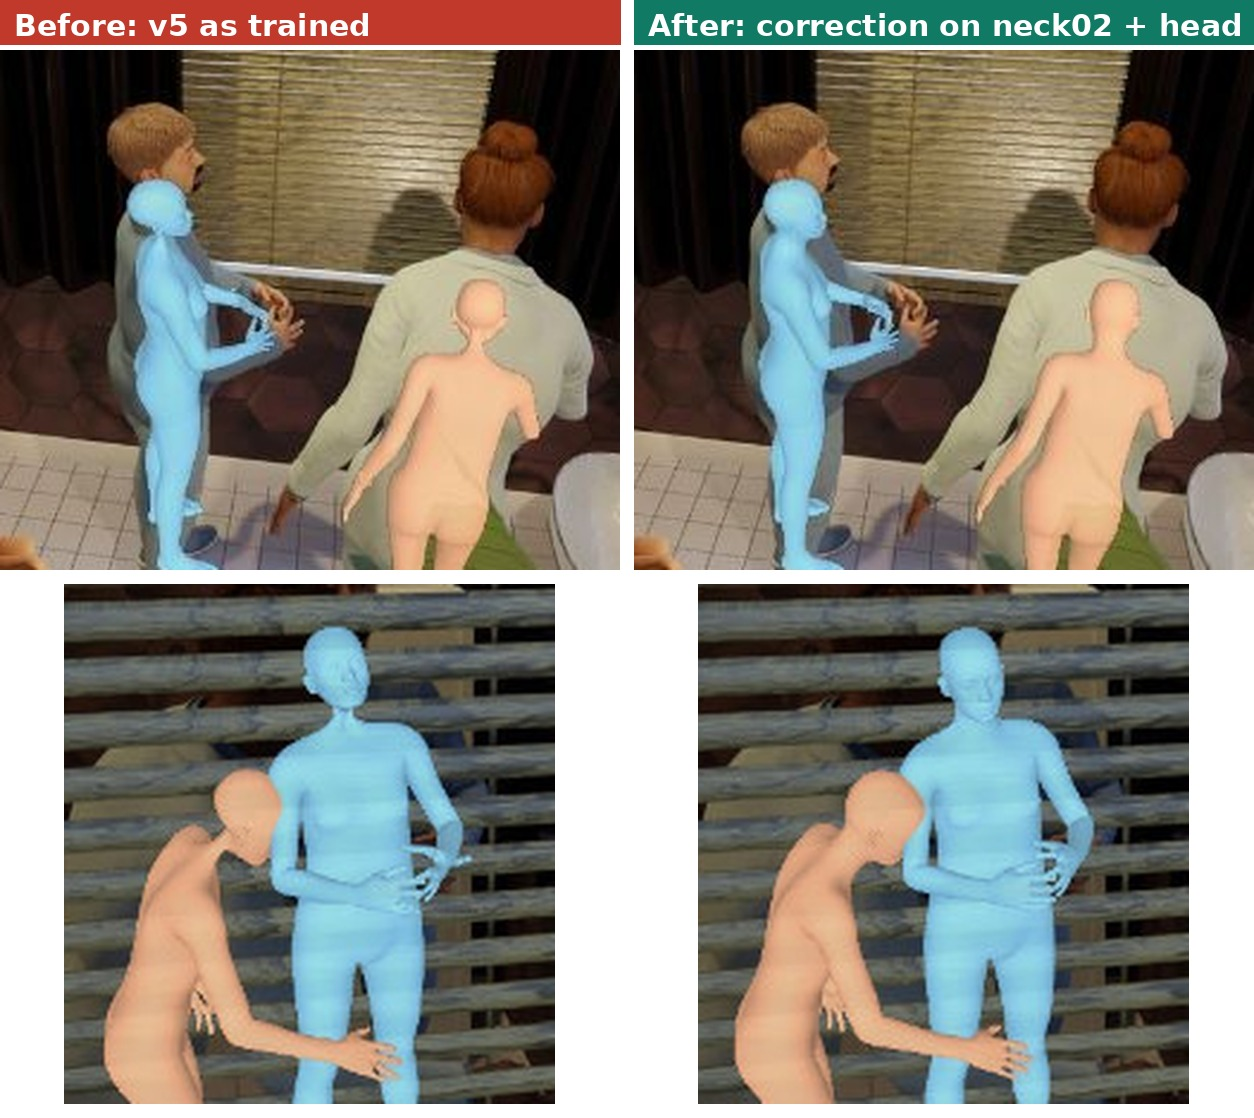
\includegraphics[width=0.62\linewidth]{figures/img/neck_before_after_v5.jpg}}%
  {\DiagPending{F6: holdout images 579862 and 579863, Base without and with the bone correction
   (docs/figures/neck\_before\_after\_v5.jpg)}}
\caption[The thin neck of Base, and the same checkpoint with the bone correction]{Holdout images 579862 (top) and
579863 (bottom). Left: Base as trained. Right: the same checkpoint with the output correction of
Section~\ref{sec:diag-neck}, no training; nothing else differs. Synthetic images, bodies at the model's own depth, so
the depth bug of Section~\ref{sec:diag-depth} still draws them too small. The correction also turns two hand bones;
only the necks were judged, by eye.}
\label{fig:neck-before-after-v5}
\end{figure}

Figure~\ref{fig:neck-before-after-v5} shows the first failure as it was seen. In the left column Base draws each neck
as a thin stalk, pinched under the head, on synthetic holdout images it never trained on. The second failure was the
hands: the predicted fingers curled into claws. From then on every real-photo demo set the fingers to rest pose. The
third failure was children. A standing boy in one of our own photos received an adult body
(Figure~\ref{fig:final-real-photos} shows him again with the final model).

The draft gave each failure a cause without a test against an alternative. For the neck it concluded that linear blend
skinning stretches the skin between Anny's stacked neck bones when the network predicts slightly different rotations
for each, ``a property of the rig, not a training failure''. A later reading blamed weak supervision on a redundant
four-bone chain, plus the depth defect. For the fingers the belief was resolution: a hand covers too few pixels. For
children the belief was that age had not been learned. The evidence was five small people in our own photos,
predicted at adult ages of \DiagSmallPeopleAgeLow{} to \DiagSmallPeopleAgeHigh. The rest of this chapter shows that the
neck explanation is wrong, that resolution explains little of the finger error, and that the child evidence was
wrong. Looked at again, four of the five ``small people'' were adults who crouched, sat or were cut off by the frame.
The skeletal height that had flagged them is measured on the posed body, so crouching shortens it, and their height
phenotype was \DiagSmallPeopleHeightLow{} to \DiagSmallPeopleHeightHigh, an adult rest body. Only the boy was a child.
He received age \DiagBoyAge{} and height phenotype \DiagBoyHeight: an adult body.

The figure does not show the fingers or the children, and it does not show a real photo; Chapter~\ref{ch:results}
has the real-image pairs. The neck widths are judged by eye; the number behind them is the neck girth of
Table~\ref{tab:neck}.

% -----------------------------------------------------------------------------
\section{What is not the cause: six structural checks}
\label{sec:diag-checks}

\begin{table}[tbp]
\centering\footnotesize
\begin{tabular}{@{}p{0.27\linewidth}p{0.2\linewidth}p{0.45\linewidth}@{}}
\toprule
check & sample & result \\
\midrule
1 ground truth decodes onto the people (no network) & manifest, 55 people &
labels render onto the people; \DiagGTInsideImage\,\% of joints inside the image, \DiagGTInsideBox\,\% inside the
box: the missing joints are truncation at the image border; dataset camera matches on 100\,\% of images \\
2 body model, rest pose and age sweep & body model only &
skeletal height \DiagAgeSweepLow\,m at age 0, \DiagAgeSweepHigh\,m at age 0.8; head/height
\DiagHeadRatioLow{} to \DiagHeadRatioHigh \\
3 single-joint moves & body model only &
all \DiagPerturbations{} pass (96--100\,\% of the moved vertices in the intended part); neck01 leaks about 4\,\% into
the shoulders, normal skinning \\
4 gradients and mesh response & 4 holdout images &
zero-gradient bones are exactly the \DiagHelperBones{} masked helpers; all \DiagActiveBones{} active bones and all
\DiagShapeOutputs{} shape outputs receive gradient; two of the three camera outputs receive none \\
5 prediction vs.\ truth; shape swap & holdout (\DiagHoldoutImages{} images, \DiagHoldoutPeople{} people), manifest &
neck length \DiagNeckLengthPct\,\% of truth; true shape with predicted pose lowers the PVE of the 10 manifest
children from \DiagChildSwapBefore{} to \DiagChildSwapAfter\,mm \\
6 capped overfit & 40 manifest training images, 400 steps &
training PVE \DiagOverfitTrainBefore{} $\to$ \DiagOverfitTrainAfter\,mm ($-$\DiagOverfitTrainDrop\,\%); holdout
\DiagOverfitHoldBefore{} $\to$ \DiagOverfitHoldAfter\,mm (+\DiagOverfitHoldRise\,\%); two warnings (text) \\
\bottomrule
\end{tabular}
\caption[Six structural checks]{Six structural checks on Base before any training change. The manifest is a fixed set
of 40 training images (10 adults, 10 children, 10 with visible hands, 10 hard neck poses) and 15 holdout images
(no children); it is excluded from every later fine-tune. Checks 1--5 are read-only; check 6 trains a throw-away copy
and reports setting V0 (helper bones unmasked).}
\label{tab:diag-checks}
\end{table}

\begin{figure}[tbp]
\centering
\IfFileExists{figures/img/gt_decode_overlay.jpg}%
  {\includegraphics[width=0.8\linewidth]{figures/img/gt_decode_overlay.jpg}}%
  {\DiagPending[0.8\linewidth]{F24: ground-truth decode overlay, AnnyOne labels rendered with the dataset camera
   (cluster: results/diagnostics/gt\_decode/vis/, two files)}}
\caption[Check 1: AnnyOne labels decoded and rendered with the dataset camera]{Check 1: AnnyOne ground-truth pose and
shape decoded through the same Anny body model as in training and drawn with the dataset camera, manifest images. No
network is involved; the meshes sit on the people.}
\label{fig:gt-decode}
\end{figure}

Table~\ref{tab:diag-checks} lists the six checks and Figure~\ref{fig:gt-decode} shows check~1. The ground truth decodes
onto the people. The share of joints inside the image and inside the annotated box move together per category, so
the missing joints are truncation, not a decoding error; the first automatic report called this a decoding defect
because its rule compared box containment with a fixed 95\,\%. The body model makes a child with child proportions,
and each of the 16 single-joint moves (neck and fingers among them) moves the intended part. The gradient check
found every active bone and every shape output reachable. Per bone the gradients range from \DiagGradRoot{} at the
root to \DiagGradFingers{} at the fingers, and the loss is dominated by shape (\DiagLossShareShape\,\%), while the
translation and distance terms take \DiagLossShareTransl\,\% and \DiagLossShareDist\,\%. On the holdout the predicted
neck has the right length, and predicted shape explains the small remainder. The capped overfit lowered the training
error by a third and raised the holdout error, as memorising must.

Read together, the checks rule out the rig, the decoding of the labels and the gradient path. The draft's four neck
tests stay valid as eliminations of the same kind: the rest-pose render looked normal, all neck bones are active in
the loss, the thin neck appears on synthetic images, and the proportions phenotype is accurate. So the cause had to be
in what training asked the network to do. The overfit test gave two warnings. First, the summed rotation loss barely
moved while the images were memorised (\DiagOverfitRotFirst{} $\to$ \DiagOverfitRotLast). Second, the translation and
2D reprojection terms rose (\DiagOverfitTranslFirst{} $\to$ \DiagOverfitTranslLast{} and \DiagOverfitTwoDFirst{}
$\to$ \DiagOverfitTwoDLast, first against last five epochs) while the pelvis-centred 3D terms fell. This was possibly a
first sign of the depth bug of the next section. It is weak evidence: each value is a single-batch print, and the
averages of the first and second half fall instead (\DiagOverfitTranslHalfA{} $\to$ \DiagOverfitTranslHalfB{} and
\DiagOverfitTwoDHalfA{} $\to$ \DiagOverfitTwoDHalfB).

The checks cannot see two kinds of fault. A target that is consistent in itself but placed at a different joint
than the model's anchor passes every check, because the checks compare pelvis-centred quantities. A bone that is
flipped the same way in every person passes too, because the checks tested the rig in isolation and averaged the
bone errors by group. Both faults were there. The holdout also has no children, so every child number in this chapter
is in-sample or from real photos.

% -----------------------------------------------------------------------------
\section{The hidden depth bug}
\label{sec:diag-depth}

\begin{table}[tbp]
\centering\footnotesize
\begin{tabular}{@{}lrr@{}}
\toprule
quantity & truth & Base \\
\midrule
pelvis depth, mean (sd)                                & \DiagDepthTrueMean\,m (\DiagDepthTrueSd) & \DiagDepthPredMean\,m (\DiagDepthPredSd) \\
linear fit of predicted on true depth                  & slope 1, intercept 0 & slope \DiagDepthSlopeBase, intercept \DiagDepthInterceptBase\,m \\
people predicted farther than truth                    & --                  & \DiagDepthFartherPct\,\% \\
correlation of true depth with depth error             & --                  & \DiagDepthCorrError \\
skeletal height (3D, metric)                           & \DiagSkelHeightTrue\,m & \DiagSkelHeightPred\,m ($r = \DiagSkelHeightCorr$) \\
drawn size, predicted over true (pixels)               & 1                   & \DiagSizeBase \\
pelvis root error (3D)                                 & 0                   & \DiagRootErrBase\,m \\
head / pelvis 2D error, median (mean)                  & 0                   & \DiagHeadPxBaseMedian{} (\DiagHeadPxBase) / \DiagPelvisPxBaseMedian{} (\DiagPelvisPxBase) px \\
correlation of PVE with depth error                    & --                  & \DiagCorrPVEDepth \\
\bottomrule
\end{tabular}
\caption[Placement of Base on the holdout]{Where Base places people. V1, 100-image AnnyOne holdout, all
\DiagHoldoutPeople{} matched people. The body has the right metric size but is placed too far away, so it is drawn
too small; PVE, which aligns the pelvis first, does not see it.}
\label{tab:diag-placement}
\end{table}

% T08 Depth fix: the depth-anchor pilots, the final model and its control (REWRITE_PLAN.md section 4, T8).
% Owner: Diagnostics writer (chapter 5, section "The hidden depth bug"); also referenced from Results 6.2.
% Setting: V1, 100-image AnnyOne holdout (579,860-579,959), matched people; root error = PLACEMENT table `root mm`
% (absolute 3D pelvis distance), never the signed `root dz`.
% Sources (handover.md 3.1 tables, checked against the logs there; head px from the deck build
% docs/deck_src/build.js:439, slide 14, and handover 3.1 for the final model and control):
%   Base (v5 00099)           3571596:55,64; 3570222:40
%   2-ep control              3571599:49,58,67-68   (pilot_root_dist1_transl1_...)
%   2-ep fix x1               3571598:66,75,84-85   (pilot_person_center_dist1_transl1_...)
%   2-ep fix x5               3572418:52,61,70-71
%   2-ep fix x20              3572483:57,66,75-76
%   10-ep control             3571934:134,143,152-153 (long_root)
%   10-ep fix x1              3571933:125,134,143-144 (long_person_center)
%   10-ep fix x5              3572482:126,135,144-145 (long_pc_dist5)
%   Control (exp7)            3611339:166,175,182-184; head px 67.1 (3611339:166)
%   Final (exp7 fix arm)      3611336:175,184,191-193; head px 7.6 (3611336:175)
%   Mixed-L e62 3571963:40,55,64; Fresh-heads-L (v10 e290) 3571794:40,55,64 (no head px quoted)
% PVE / recall rounded to one decimal from the handover's two-decimal values (72.19 -> 72.2, 77.25 -> 77.3 as on the deck).
\begin{table}[htbp]
\centering\footnotesize
\setlength{\tabcolsep}{3pt}
\begin{tabular}{@{}lrrrrrrrr@{}}
\toprule
run (depth loss) & root (m) & size & slope & icpt.\ (m) & head px & pelvis px & PVE & recall \\
\midrule
Base & 1.21 & 0.63 & 0.33 & 2.36 & 64.5 & 23.4 & 70.5 & 90.2 \\
\addlinespace
\multicolumn{9}{@{}l}{\emph{2-epoch fine-tunes of Base, AnnyOne only}} \\
control $\times$1 & 1.11 & 0.66 & 0.33 & 2.28 & 58.1 & 23.3 & 72.3 & 89.8 \\
fix $\times$1 & 0.69 & 0.78 & 0.30 & 1.93 &  9.6 & 37.3 & 77.3 & 87.8 \\
fix $\times$5 & 0.66 & 0.80 & 0.44 & 1.62 &  8.5 & 38.1 & 76.8 & 87.8 \\
fix $\times$20 & 0.53 & 0.87 & 0.43 & 1.44 &  8.8 & 31.4 & 75.7 & 87.4 \\
\addlinespace
\multicolumn{9}{@{}l}{\emph{10-epoch fine-tunes of Base, AnnyOne only}} \\
control $\times$1 & 1.44 & 0.59 & 0.34 & 2.59 & 64.0 & 24.3 & 72.2 & 89.4 \\
fix $\times$1 & 0.73 & 0.78 & 0.30 & 1.98 &  7.6 & 38.5 & 75.5 & 87.0 \\
fix $\times$5 & 0.54 & 0.84 & 0.38 & 1.59 &  7.2 & 33.1 & 74.8 & 87.8 \\
\addlinespace
\multicolumn{9}{@{}l}{\emph{10-epoch fine-tunes of Base with 30\% 3DPW (v23 labels)}} \\
Control $\times$1 & 1.40 & 0.59 & 0.28 & 2.66 & 67.1 & 26.7 & 77.4 & 89.0 \\
Final $\times$5 & 0.73 & 0.78 & 0.42 & 1.75 &  7.6 & 41.1 & 73.7 & 87.0 \\
\addlinespace
\multicolumn{9}{@{}l}{\emph{other checkpoints trained with pelvis targets}} \\
Mixed-L & 1.39 & 0.59 & 0.31 & 2.60 &  --  & 25.1 & 75.0 & 88.6 \\
Fresh-heads-L & 1.49 & 0.57 & 0.28 & 2.71 &  --  & 24.0 & 74.1 & 89.0 \\
\bottomrule
\end{tabular}
\caption[Depth fix: pilots, final model and control]{Placement before and after building the training targets at
the head joint. V1, 100-image AnnyOne holdout, matched people. Root error: absolute 3D distance of the pelvis; size:
predicted over true head-to-pelvis distance in pixels (1 is right); slope and intercept: linear fit of predicted
against true pelvis depth (1 and 0\,m are right); head and pelvis px: 2D error of those joints; PVE in mm, recall in \%. Control
rows build the targets at the pelvis, fix rows at the head; $\times$1/5/20: weight of the distance and translation
terms. Final also has the bone correction. One run per row, no seed. No control was run at
$\times$5 or $\times$20; each fix row is read against the control of the same length.}
\label{tab:depth-runs}
\end{table}


Table~\ref{tab:diag-placement} is the placement section of the holdout trace. True pelvis depths average
\DiagDepthTrueMean\,m; Base predicts \DiagDepthPredMean\,m with a smaller spread. A straight-line fit gives predicted
$= \DiagDepthSlopeBase \times \text{true} + \DiagDepthInterceptBase$\,m (Figure~\ref{fig:depth-scatter}). All
\DiagHoldoutPeople{} people are placed too far, and the nearest are pushed farthest (correlation
\DiagDepthCorrError). The 3D skeleton has the right height, so a body of the right size sits at the wrong distance and
is drawn at \DiagSizeBase{} of its true size. Its pelvis lands near the right pixel, its head does not. PVE is blind to
all of this: its correlation with the depth error is \DiagCorrPVEDepth.

The trace was not the only sign. The gradient check had shown that two of the three camera outputs receive no
gradient, and the overfit test had shown the translation and 2D terms rising. A read of the training code gave the
mismatch. The model places each mesh by its head joint and reports the head as its
position, but the training code built the translation, distance, detection-cell and offset targets at joint 0, the
pelvis. A one-batch debug print confirmed it: the predicted vertical offsets were \DiagOffsetMin{} to
\DiagOffsetMax{} cells where the legal range is $\pm$0.5. The likely mechanism, which I did not test on its own, is
this. The detection and offset terms pull the anchor pixel toward the pelvis, while the mesh hangs from that pixel by
its head, so every projected joint is displaced by the head-to-pelvis distance in pixels. The 2D terms are the only
strong terms that see depth, because the 3D joint and vertex terms are pelvis-centred. They can shrink the
displacement only by drawing the body smaller, that is, by predicting it farther away. The distance and translation
terms, \DiagLossShareDepthTerms\,\% of the loss, could not resist. Near people have the largest head-to-pelvis
distance in pixels and were pushed farthest, which matches the correlation above. Building the targets at the head
(Chapter~\ref{ch:method}) is the fix; Table~\ref{tab:depth-runs} is its test.

In Table~\ref{tab:depth-runs} all five fix runs reach a root error of \DiagRootErrFixLow--\DiagRootErrFixHigh\,m, and
both pelvis-target controls with the same schedule stay at \DiagRootErrCtrlLow--\DiagRootErrCtrlHigh\,m. The drawn size
rises from \DiagSizeCtrlLow--\DiagSizeCtrlHigh{} to \DiagSizeFixLow--\DiagSizeFixHigh, and the head lands within 7 to
10 pixels instead of 58 to 67. The final model keeps the fix with 30\,\% real images and the bone correction in
training: root error \DiagFinalRootErr{} against \DiagControlRootErr\,m for its Control, size \DiagFinalSize{} against
\DiagControlSize, slope \DiagFinalSlope{} against \DiagControlSlope. These gaps are far above the run-to-run variation:
every fix run lies below every control. Two checkpoints trained with pelvis targets, Base+3DPW (old labels) and a
fresh-head run, carry the same bug (\DiagOldRootErrA{} and \DiagOldRootErrB\,m). The bug stayed hidden for two reasons.
PVE and PA-PVE align the pelvis before measuring. The real-photo demos place every body from its detection box, so
only the synthetic demo and the trace panels ever used the model's own depth.

The table does not show a solved depth. The fix moved the offset and the body size, not the slope (Final: \DiagFinalSlope): \DiagSlopeSwitch{}
with the switch alone and \DiagSlopeStrongLow--\DiagSlopeStrongHigh{} with a stronger depth loss, far from 1.
Predictions are still pulled toward about 2.5 to 2.9\,m, for a reason I have not found. The pelvis 2D error rose from
about 23 to 31--41 pixels; the likely reason is that the head is now pinned while the body is still drawn too small,
which was not checked. Every fix run is also worse than its control on PVE (+\DiagFixCostPVELow{} to
+\DiagFixCostPVEHigh\,mm) and recall ($-$\DiagFixCostRecallLow{} to $-$\DiagFixCostRecallHigh{} points). Each gap is
within run-to-run variation, but all five point the same way, so I report them as a likely cost. By the success rule
written before the pilots ran (PVE at most 71.5\,mm and recall at least 89.2\,\%), every run failed, the controls
included.

% -----------------------------------------------------------------------------
\section{The neck: a per-bone dump}
\label{sec:diag-neck}

\begin{table}[tbp]
\centering\footnotesize
\begin{tabular}{@{}lrrrl@{}}
\toprule
bone & local error (deg) & global error (deg) & verdict & note \\
\midrule
neck01 & \DiagDumpNeckOne   & --    & OK          & \\
neck02 & \DiagDumpNeckTwo   & --    & half-turn   & twist \DiagDumpNeckTwoTwist\,deg about its own axis, swing \DiagDumpNeckTwoSwing\,deg \\
neck03 & \DiagDumpNeckThree & \DiagDumpNeckThreeGlobal & OK locally & carries neck02's turn \\
head   & \DiagDumpHead      & \DiagDumpHeadGlobal      & half-turn   & turns the chain back \\
jaw    & \DiagDumpJaw       & --    & OK          & \\
\bottomrule
\end{tabular}
\caption[Per-bone dump of the neck chain]{Per-bone dump of Base's neck chain. V1, 100-image AnnyOne holdout,
\DiagHoldoutPeople{} people; medians. Local error: relative to the parent bone; global error: of the bone's orientation
in the camera frame. A half-turn is an error above 150\,deg in at least half the people.}
\label{tab:diag-neck-dump}
\end{table}

% T09 Neck: the bone correction without training, with a 2-epoch fine-tune, and in the final model
% (REWRITE_PLAN.md section 4, T9). Owner: Diagnostics writer (5.4); also referenced from Results 6.3.
% Setting: V1, 100-image AnnyOne holdout, 222 people, matched people.
% Sources: columns 1-4 = exp6 on v5, job 3579014:101-114 (handover 3.2 table and 0b);
%          column 5 = exp7 control 3611339:182-198; column 6 = final model 3611336:191-207 (handover 3.2, 5/7).
% Rows: neck02 :101 / :193,:197 / :202,:206; head :103 / :194,:198 / :203,:207; metacarpal1.L, finger4-1.R :105-106 /
%   3611339:195-196 / 3611336:204-205; girth :107 / :189 / :198; PVE_neck :108 / :190 / :199; PVE :109 / :182 / :191;
%   PA-PVE :110; recall :112; global head :113 / :191 / :200; fingers :114 / :192 / :201.
% "not dumped" = the holdout dump 3573518 did not cover finger bones; finger4-1.R was found on the training images.
% Correction constants 178.8 / 179.2 / 179.8 / 179.7 deg (3579014:12, :37), from 200 training images.
\begin{table}[htbp]
\centering\footnotesize
\setlength{\tabcolsep}{3pt}
\newcommand{\hd}[1]{\begin{tabular}[b]{@{}c@{}}#1\end{tabular}}
\begin{tabular}{@{}lrrrrrr@{}}
\toprule
 & \hd{Base} & \hd{corr.,\\no train.} & \hd{corr.\ +\\2-ep.\ FT} & \hd{2-ep.\\control}
 & \hd{Control\\10 ep.} & \hd{Final\\10 ep.} \\
\midrule
neck02 (deg)         & 175.6 &   4.5 &   4.7 & 175.7 & 175.8 &   4.8 \\
head bone (deg)      & 177.9 &  12.4 &  11.2 & 177.9 & 177.7 &   8.9 \\
metacarpal1.L (deg)                 & 180.0 &   0.0 &   0.0 &  --   & 180.0 &   0.0 \\
finger4-1.R (deg)                   & n.d.  &  10.2 &  10.3 &  --   & 180.0 &   9.6 \\
neck girth, pred./true& 0.461 & 1.004 & 0.997 & 0.461 & 0.464 & 0.996 \\
PVE$_\text{neck}$ (mm) & 27.3 & 10.8 & 10.7 & 27.9 & 27.7 & 11.0 \\
\addlinespace
body PVE (mm)                       &  70.5 &  71.3 &  68.8 &  76.9 &  77.4 &  73.7 \\
PA-PVE (mm)                         &  53.3 &  52.2 &  50.9 &  55.2 &  56.4 &  50.3 \\
recall (\%)                         &  90.2 &  90.2 &  89.4 &  91.1 &  89.0 &  87.0 \\
head direction (deg)         &  12.0 &  19.1 &  14.4 &  13.8 &  13.0 &  13.1 \\
fingers (deg)                       &  17.3 &   8.2 &   8.3 &  17.4 &  17.4 &   8.3 \\
\bottomrule
\end{tabular}
\caption[Neck: the half-turned bones and their correction]{The two half-turned neck bones and their correction. V1,
100-image AnnyOne holdout, matched people. Bone errors are local (relative to the parent bone) medians; about 180\,deg
means the bone is turned half a turn. Girth: radius of the neck skin, predicted over true. PVE$_\text{neck}$: vertex
error over the 171 neck-skin vertices, centred at neck01. Corr.: one constant rotation per flipped bone
(neck02, head, metacarpal1.L, finger4-1.R), estimated on 200 training images. FT: fine-tune. The 2-epoch columns are AnnyOne-only fine-tunes of Base; Control and Final are the 10-epoch runs with 30\% 3DPW, Final also with the depth fix. n.d.: not
dumped on the holdout. One run per column, no seed; PVE gaps below about 10\,mm are within run-to-run variation
(Table~\ref{tab:pilot-noise}).}
\label{tab:neck-bones}
\end{table}


Table~\ref{tab:diag-neck-dump} is the dump that found the neck fault. neck02 is wrong by \DiagDumpNeckTwo\,deg, a
half-turn about its own axis, and the head bone by \DiagDumpHead\,deg. neck03 is right relative to its parent but
\DiagDumpNeckThreeGlobal\,deg off in the camera frame, because it inherits neck02's turn. The two half-turns cancel, so
the head points the right way (\DiagDumpHeadGlobal\,deg) and PVE never showed the fault. The skin between them is
twisted thin: the neck girth is \DiagNeckGirthBase{} of the truth and the neck-skin error \DiagNeckSkinBase\,mm
(Table~\ref{tab:neck}). The earlier figures of 62.7\,deg for the neck and 89.5\,deg for the head were group means
over these bones; they hid the flip and suggested weak supervision. The same flip is in all eight checkpoints of the
Base line: the three training stages before Base, Base, Base+3DPW, the 10-epoch depth-fix pilot and two pilots with
a geodesic rotation loss (neck02 \DiagNeckTwoRangeLow--\DiagNeckTwoRangeHigh\,deg, girth
\DiagGirthRangeLow--\DiagGirthRangeHigh). It is present from the first stage, which trained fresh heads on a frozen
backbone, before the helper mask, the neck boost and the shape weight of 20 were introduced. The depth-fix pilot keeps
girth \DiagGirthRangeLow, so depth is not the cause of the neck. A fresh-head run started from the same pretrained
backbone has a normal neck (girth \DiagFreshGirth, neck-skin error \DiagFreshNeckSkin\,mm), but flips other bones: a
compensated pair in the left arm (shoulder01.L and upperarm02.L) and three metacarpals.

This refutes the draft's explanation. The rig is fine: all 16 single-joint moves pass. The rest-pose render, which had
seemed to support skin stretch, is explained just as well by the flip, because rest pose sets every rotation to the
identity and so removes both half-turns. Only the per-bone dump separates the two explanations. The ground-truth
rotation blocks are all proper rotations, and every checkpoint uses the same local-bone pose parameterisation. A loss
weight cannot undo a half-turn. The neck boost of the earlier stage is $\times$2.41 for the boosted bones and
$\times$0.60 for the rest after renormalisation, and it left the neck unchanged. A geodesic rotation loss moved neck02
only from \DiagNeckTwoBase{} to \DiagGeodesicNeckTwo\,deg in 2 epochs. The likely reason is that neck02 and the head
must turn back together, and any partial turn raises the loss. So I corrected the output instead: one constant
rotation $C_b$ per flipped bone, applied as $R_b \leftarrow R_b C_b$ after the rotation decoding, estimated on 200
training images and never on the holdout (Chapter~\ref{ch:method}). The constants are \DiagCorrNeckTwo,
\DiagCorrHead, \DiagCorrMetacarpal{} and \DiagCorrFinger\,deg for neck02, head, metacarpal1.L and finger4-1.R.

Table~\ref{tab:neck} reads as follows. Without training the correction turns neck02 back to \DiagNeckTwoNoTrain\,deg
and restores the girth (\DiagGirthNoTrain) and the neck-skin error (\DiagNeckSkinNoTrain\,mm). The head direction gets
worse, \DiagHeadDirBase{} to \DiagHeadDirNoTrain\,deg, above the 15-degree limit set before the run. The likely reason
is the compensated chain: the head's error differs from person to person, so one constant cannot undo it. After a
2-epoch fine-tune with the correction in place the head direction is \DiagHeadDirFineTune\,deg, against
\DiagHeadDirCtrlTwo\,deg for the control, which keeps the flip. Body PVE reads \DiagPVEBase{}, \DiagPVENoTrain{} and
\DiagPVEFineTune\,mm against \DiagPVECtrlTwo\,mm for the control. That gap is within run-to-run variation, and the
control sits above the range of six earlier arms, so the result is no sign of a PVE cost, not a gain. The final model
keeps the correction through 10 epochs with real images: neck02 \DiagFinalNeckTwo\,deg, head \DiagFinalHeadBone\,deg,
girth \DiagFinalGirth, neck-skin error \DiagFinalNeckSkin\,mm, head direction \DiagFinalHeadDir{} against
\DiagControlHeadDir\,deg for Control.

\begin{figure}[tbp]
\centering
\begin{subfigure}[t]{0.48\linewidth}\centering
\IfFileExists{figures/img/exp6_compare_579864.jpg}%
  {\includegraphics[width=\linewidth]{figures/img/exp6_compare_579864.jpg}}%
  {\DiagPending[0.95\linewidth]{F23a: holdout 579864, without (top) and with (bottom) the correction
   (cluster: exp6 compare/579864.jpg)}}
\caption{holdout image 579864}
\end{subfigure}\hfill
\begin{subfigure}[t]{0.48\linewidth}\centering
\IfFileExists{figures/img/exp6_compare_579866.jpg}%
  {\includegraphics[width=\linewidth]{figures/img/exp6_compare_579866.jpg}}%
  {\DiagPending[0.95\linewidth]{F23b: holdout 579866, without (top) and with (bottom) the correction
   (cluster: exp6 compare/579866.jpg)}}
\caption{holdout image 579866}
\end{subfigure}
\caption[Bone correction on two more holdout images]{Two more holdout images, Base without (top row) and with
(bottom row) the bone correction, no training, bodies at the model's own depth. Synthetic; judged by eye; the depth
bug is still present.}
\label{fig:exp6-compare}
\end{figure}

What is not shown: why the bones flipped. The 6D start value of the rotation output is singular and starts a bone
tilted about its local $x$ axis; that fits the tilted metacarpal1.L but not the twist of neck02, so the origin is
unknown. The correction adds no parameters, and it says nothing about the origin. A two-sided correction, needed to
keep a compensated chain such as the fresh-head run's left arm intact, was not implemented. On real photos there is no
neck ground truth; the real-image pairs (Figure~\ref{fig:neck-3dpw}) are judged by eye, and there the fixed model also
had the 2-epoch fine-tune.

% -----------------------------------------------------------------------------
\section{The fingers}
\label{sec:diag-fingers}

% T10 Fingers (REWRITE_PLAN.md section 4, T10). Owner: Diagnostics writer (5.5); also referenced from Results 6.4.
% Setting: V1, 100-image AnnyOne holdout, matched people; finger error = mean local rotation error over the finger bones.
% Sources: predicted 17.3 / rest 15.1 (3571960:290; findings "Fingers"); test-time crop x1.3 17.2, body PVE 124.8
%   (3571960:294-299); region-normalised loss 17.5 vs control 17.4 (3571959:316; 3571960:314); bone correction no
%   training 8.2 (3579014:114); + 2-ep fine-tune 8.3 (3579014:114); final 8.3 vs control 17.4 (3611336:201;
%   3611339:192); Fresh-heads-L (v10) three metacarpals 32.0 -> 17.8 (3579015:80).
%   Hand size: 2.25 tokens median at 672 px, 41% under 2 tokens (3571960:287); person crop 4.2 / 0%, children's hands
%   0.7 / 80% (deck slide 17, D slide 17).
%   Hands' share of the rotation loss ~70% (with x4 boost) -> 33% (deck notes slide 17, handover 3.3).
\begin{table}[!htb]
\centering\footnotesize
\begin{tabular}{@{}lrr@{}}
\toprule
\multicolumn{3}{@{}l}{\emph{(a) finger rotation error on the holdout}} \\
setting & fingers (deg) & reference (deg) \\
\midrule
Base, predicted fingers                                   & 17.3 & -- \\
Base, fingers set to rest pose                             & 15.1 & -- \\
Base, test-time person crop (PVE 124.8\,mm) & 17.2 & 17.3 (paired) \\
region-normalised rotation loss, 2 ep. & 17.5 & 17.4 (control) \\
Base + bone correction, no training                        &  8.2 & 17.3 (Base) \\
Base + bone correction, 2-ep.\ fine-tune &  8.3 & 17.4 (control) \\
Final (10 ep., 30\% 3DPW)                                  &  8.3 & 17.4 (Control) \\
Fresh-heads-L, three metacarpals corrected & 17.8 & 32.0 (uncorr.) \\
\midrule
\multicolumn{3}{@{}l}{\emph{(b) hand size in tokens (14-px patches of the 672-px input)}} \\
 & median length & under 2 tokens \\
\midrule
full image, all hands       & 2.25 & 41\% \\
person crop at test time    & 4.2  &  0\% \\
children's hands, full image & 0.7  & 80\% \\
\bottomrule
\end{tabular}
\caption[Fingers: what changed the finger error]{Fingers. (a) Finger rotation error, V1, 100-image AnnyOne holdout,
matched people; the reference is the matching run without the change. Rest pose keeps the metacarpals predicted, so
the 15.1\,deg still contains the flipped metacarpal1.L. (b) Hand length in input tokens. One run per row, no seed.}
\label{tab:fingers}
\end{table}


Table~\ref{tab:fingers} collects every finger measurement. Predicted fingers are \DiagFingersBase\,deg off; fingers set
to rest pose are \DiagFingersRest\,deg off, so the prediction was worse than no prediction. Hands are small: the
median hand is \DiagHandTokens{} tokens long in the 672-pixel input and \DiagHandUnderTwo\,\% of hands are shorter than
two tokens. A person crop at test time raises the median to 4.2 tokens, but the finger error stays at \DiagFingersZoom\,deg
while body PVE nearly doubles to \DiagZoomPVE\,mm, because the model never saw such a camera. A region-normalised
rotation loss gave \DiagFingersRegion\,deg against \DiagFingersRegionCtrl\,deg for its control. The per-bone search on
200 training images then found two hand bones turned half a turn, metacarpal1.L (180\,deg) and finger4-1.R
(178.8\,deg). Correcting them lowers the finger error to \DiagFingersFixNoTrain\,deg without training and
\DiagFingersFixFT\,deg after the fine-tune; the final model holds \DiagFingersFinal{} against
\DiagFingersControl\,deg for Control.

About half the finger error was therefore two flipped bones, not resolution. The resolution belief was tested only by
test-time zoom, which did not help; a hand-crop branch was never tested. The region-normalised loss cut the hands'
share of the rotation loss from about 70\,\% (with the neck and hand boost) to 33\,\%, so it was a rebalance, not an
upweighting. The gradient check had shown the smallest gradients of any bone group at the fingers and the worst
conditioning of their 6D outputs; whether the fingers are also under-trained is a guess I did not test.

Predicted fingers have not been shown on a real photo: every demo so far sets them to rest pose. Rest pose keeps the
metacarpals predicted, so the \DiagFingersRest\,deg still contains the metacarpal1.L flip, and a rest-pose floor with
the correction was not measured. The split of the 9.1-degree drop between the two bones was not measured either.

% -----------------------------------------------------------------------------
\section{Children and body shape}
\label{sec:diag-children}

% T18 Shape head: shape weight 1 vs 20, plus the regression to the median in the tails
% (REWRITE_PLAN.md section 4, T18). Owner: Diagnostics writer (5.6).
% Part (a): the draft's tab:shape as is (main.tex:980-998), n = 10 holdout images (plan 1.7); "fixed" softened to
%   "near the mode"; v4 = the stage before Base (alpha_shape 1, boosted_v4 00299), v5 = Base (alpha_shape 20).
% Part (b): holdout GT age 0.6-0.8 (n = 53, mean 0.67) predicted 0.57 (3570222:89); full holdout near the mode
%   age bias -0.015 / abs 0.037, gender -0.008 / 0.068 (3570222:75); in-sample babies (youngest 50, GT age 0.015)
%   predicted 0.10 (3569950:61; 3571955:174-175), height -0.25 traded (3569950:61,76); training medians gender 0.588,
%   age 0.601, height 0.500 (3569948:8-18); holdout youngest person 0.513 (3569948:33).
\begin{table}[htbp]
\centering\footnotesize
\begin{tabular}{@{}lrrrrl@{}}
\toprule
\multicolumn{6}{@{}l}{\emph{(a) predicted minus true phenotype, 10 holdout images (draft measurement)}} \\
phenotype & true mean & true std & weight 1 & weight 20 (Base) & reading \\
\midrule
age         & 0.553 & 0.036 & $+0.199$ & $-0.002$ & near the mode \\
height      & 0.579 & 0.026 & $-0.154$ & $-0.026$ & near the mode \\
proportions & 0.763 & 0.070 & $-0.017$ & $-0.001$ & near the mode \\
firmness    & 0.757 & 0.039 & $-0.167$ & $-0.190$ & unchanged \\
gender      & 0.694 & --    & $-0.042$ & $-0.063$ & $\approx$ \\
weight      & 0.382 & --    & $+0.056$ & $+0.064$ & $\approx$ \\
\midrule
\multicolumn{6}{@{}l}{\emph{(b) Base on the full holdout and in the young tail}} \\
\multicolumn{3}{@{}p{0.47\linewidth}}{holdout, all 222 people (nobody younger than 0.513)} & \multicolumn{3}{p{0.38\linewidth}}{age bias $-0.015$ (abs.\ 0.037); gender $-0.008$ (0.068)} \\
\multicolumn{3}{@{}p{0.47\linewidth}}{holdout, true age 0.6--0.8 ($n = 53$, mean 0.67)} & \multicolumn{3}{p{0.38\linewidth}}{predicted age 0.57} \\
\multicolumn{3}{@{}p{0.47\linewidth}}{50 youngest training people (in-sample, true age 0.015)} & \multicolumn{3}{p{0.38\linewidth}}{predicted age 0.10; height $-0.25$} \\
\multicolumn{3}{@{}p{0.47\linewidth}}{training medians (AnnyOne)} & \multicolumn{3}{p{0.38\linewidth}}{gender 0.588, age 0.601, height 0.500} \\
\bottomrule
\end{tabular}
\caption[Shape head: shape weight and the pull to the median]{Shape head. (a) The draft's comparison of the stage
before Base (shape loss weight 1) with Base (weight 20) on the same 10 AnnyOne holdout images, in phenotype units
$[0,1]$; it holds near the mode of the data only. (b) Base, V1, on the full 100-image holdout and on the 50 youngest
training people (in-sample: the holdout has no children). Predictions in both tails move toward the training median.}
\label{tab:shape-head}
\end{table}


Table~\ref{tab:shape-head}(a) is the draft's shape-weight test, measured on 10 holdout images. Raising the shape loss
weight from 1 to 20 moved the age bias from \DiagShapeAgeBiasOld{} to \DiagShapeAgeBiasNew{} and the height bias from
\DiagShapeHeightBiasOld{} to \DiagShapeHeightBiasNew; firmness did not respond. Part~(b) shows where this holds. On
all \DiagHoldoutPeople{} holdout people the head is accurate near the mode (age bias \DiagAgeBiasHoldout, absolute
error \DiagAgeAbsHoldout), but the holdout has nobody younger than \DiagHoldoutMinAge. In both tails predictions move
toward the training median: true ages of 0.6 to 0.8 are predicted at \DiagTailOldPred, and the 50 youngest training
people, at true age \DiagBabyAgeTrue, at \DiagBabyAgePred, with the height phenotype lowered to reach the right size.
On real photos Base reads children as short adults. On the Relative Human validation split (Table~\ref{tab:relhuman})
kids get a mean predicted age of \DiagRHKidAge, babies \DiagRHBabyAge{} and adults \DiagRHAdultAge; the child-versus-adult
AUC is \DiagRHAUC, near chance; none of \DiagRHKids{} kids and \DiagRHBabiesBelow{} of \DiagRHBabies{} babies fall below the
child threshold of 0.45. Their smallness goes into height instead (adults \DiagRHAdultHeight, kids \DiagRHKidHeight,
babies \DiagRHBabyHeight). Gender carries no signal either: men \DiagRHMenGender, women \DiagRHWomenGender, accuracy
\DiagRHGenderAcc\,\%. On our own demo photos the medians of all 299 shape lines are gender \DiagDemoGenderMedian, age
\DiagDemoAgeMedian{} and height \DiagDemoHeightMedian, the training medians \DiagTrainGenderMedian{} /
\DiagTrainAgeMedian{} / \DiagTrainHeightMedian. Their age spread is also narrow (standard deviation
\DiagDemoAgeStd{} against \DiagTrainAgeStd{} in training), but that alone is not evidence: the 299 lines are about 30
people, nearly all adults, each counted several times, and an adult sample must have a narrower age spread than
AnnyOne. Only the gender spread is evidence: 14\,\% of the lines lie below 0.5 although men dominate the frames.

The children and the female-looking men are one failure: when image cues are weak, the shape head returns the
training median. Two mechanisms fit and the evidence cannot rank them. One is the gap between synthetic and real
images. The other is the loss: an L1 on sigmoid outputs regresses to the median, the gradient through the sigmoid,
$s(1-s)$, is 0.25 at $s = 0.5$ but 0.015 at $s = 0.015$, and children are rare (\DiagChildShare\,\% of training people
below age 0.3, about \DiagChildBatchShare\,\% of supervised people per batch). The converted 3DPW labels pin age at
0.55 and add no child signal. How Anny makes a child explains why ``short adult'' is the failure mode. Age blends
five shapes at anchors $-1/3$, 0, 1/3, 2/3 and 1 (newborn, baby, child, young, old), and the child shape change happens
below about 0.4 to 0.5. The child cue is narrow shoulders relative to the head: shoulder over head width is
\DiagShoulderHeadChild{} at age 0.1 and \DiagShoulderHeadAdult{} at age 0.6. A small height value at age 0.6 gives a
short, broad-shouldered adult (the smallest is \DiagSmallestAdult\,m tall), and the proportions phenotype cannot make
a child (leg over stature changes by \DiagProportionsLeg). Only a lower age gives a child shape.

Not shown: children on held-out synthetic images, since the holdout has none; which of the two mechanisms dominates;
ages in years, which I never quote because the code base uses three age scales that disagree. The shape-weight test
of part~(a) has $n = 10$ and holds near the mode only. Chapter~\ref{ch:results} reports a measured improvement on
Relative Human with the final model, not a solution.

% -----------------------------------------------------------------------------
\section{Pilot noise and restart cost}
\label{sec:diag-noise}

% T14 Pilot noise and restart cost (REWRITE_PLAN.md section 4, T14). Owner: Diagnostics writer (5.7).
% Setting: V1, 100-image AnnyOne holdout, matched people; 2-epoch fine-tunes of v5 00099 (Base), lr 1e-5.
% Sources: handover 3.6; deck slide 22. Two identical configs: exp3 control 3571958:104 (PVE 76.3, head 13.6, :99) and
%   exp4 control 3571960:320 (PVE 68.7, head 11.7, :318); recall 0.8 points apart. Six 2-epoch v5-recipe arms:
%   docs/experiments_plan.md:413-419. Restart cost ~2.4 mm (controls mean 72.9 vs v5 70.5; deck notes slide 22).
%   Root error: every fix run 0.53-0.73 m, every control 1.11-1.44 m (handover 3.1). exp5 L1 control 76.9 (3573521:98).
%   train.py sets no random seed.
\begin{table}[!htb]
\centering\footnotesize
\begin{tabular}{@{}p{0.27\linewidth}p{0.36\linewidth}p{0.3\linewidth}@{}}
\toprule
quantity & measured & one run resolves \\
\midrule
two identical controls: PVE & 76.3 vs.\ 68.7\,mm (7.6\,mm) & about 10\,mm \\
\quad head direction & 13.6 vs.\ 11.7\,deg (1.9\,deg) & about 3\,deg \\
\quad recall & 0.8 points apart & about 2 points \\
six arms, Base recipe & \multicolumn{2}{@{}l@{}}{PVE 68.7--76.3\,mm, recall 88.6--90.2\,\%, head 11.3--13.7\,deg} \\
restart cost & 72.9 vs.\ 70.5\,mm for Base (2.4\,mm) & read against own control \\
root error & no measured floor & fix 0.53--0.73, control 1.11--1.44\,m \\
\bottomrule
\end{tabular}
\caption[Pilot noise and restart cost]{Run-to-run variation of the 2-epoch pilots (fine-tunes of Base at learning
rate $10^{-5}$, no seed). V1, 100-image AnnyOne holdout, matched people. Restart cost: what two more epochs of
fine-tuning Base cost with nothing changed.}
\label{tab:pilot-noise}
\end{table}


Table~\ref{tab:pilot-noise} gives the variation every pilot is read against. Two 2-epoch runs of the same
configuration differed by \DiagNoisePVE\,mm PVE (\DiagNoisePVEA{} against \DiagNoisePVEB), \DiagNoiseHead\,deg global
head direction and \DiagNoiseRecall{} recall points. Six 2-epoch arms of the Base recipe span
\DiagSixArmsPVELow--\DiagSixArmsPVEHigh\,mm PVE. Restarting a fine-tune of Base with nothing changed costs about
\DiagRestartCost\,mm (mean of the controls \DiagControlsMean{} against \DiagPVEBase\,mm).

One pilot therefore resolves about 10\,mm PVE, 3\,deg of head direction and 2 recall points. It can detect the
changes this chapter relies on: the root error (every fix run below every control), the bone angles (175 to 5\,deg),
the neck girth (0.46 to 1.00) and the finger error (17.3 to 8.3\,deg). It cannot detect a PVE change of a few
millimetres, so the costs of the depth fix and the PVE of the neck pilot stay unresolved. Because of the restart cost,
a pilot is never read against Base alone, only against its own control.

The table has no bootstrap intervals, the root error has no measured floor, and the training code sets no random
seed, so a repeated run is a repeat, not a seeded run.

% -----------------------------------------------------------------------------
\section{What did not work}
\label{sec:diag-negative}

\begin{table}[tbp]
\centering\footnotesize
\begin{tabular}{@{}p{0.2\linewidth}p{0.3\linewidth}p{0.42\linewidth}@{}}
\toprule
change & result & reading \\
\midrule
age-balanced sampler (children per batch \DiagSamplerBefore\,\% $\to$ \DiagSamplerAfterLow--\DiagSamplerAfterHigh\,\%) &
10 manifest children PVE \DiagSamplerChildPVE{} vs.\ \DiagSamplerChildPVECtrl\,mm; baby age floor \DiagSamplerBabyBefore{} $\to$ \DiagSamplerBabyAfter &
inconclusive after 2 epochs ($n = 10$, in-sample); no mechanism for real photos \\
global head orientation loss & head direction \DiagGlobalHeadArm{} vs.\ \DiagGlobalHeadCtrlA{} and \DiagGlobalHeadCtrlB\,deg (two identical controls) &
within run-to-run variation; neck bones unchanged \\
region-normalised rotation loss (hands) & fingers \DiagFingersRegion{} vs.\ \DiagFingersRegionCtrl\,deg & no effect \\
geodesic rotation loss & neck02 \DiagNeckTwoBase{} $\to$ \DiagGeodesicNeckTwo\,deg; head \DiagDumpHead{} $\to$ \DiagGeodesicHead\,deg & cannot undo a half-turn \\
neck and hand boost $\times$4 & renormalised to $\times$2.41 / $\times$0.60; neck unchanged & a loss weight on a flipped bone \\
depth loss $\times$20 & root error \DiagXTwentyRoot\,m in 2 epochs, \DiagXFiveTenRoot\,m for $\times$5 in 10; slope \DiagXTwentySlope{} vs.\ \DiagXFiveTwoSlope{} for $\times$5 in 2 epochs &
no gain over $\times$5; the 10-epoch $\times$20 run was never confirmed \\
\bottomrule
\end{tabular}
\caption[Pilots that did not work]{Changes that did not fix a failure. V1, 100-image AnnyOne holdout unless stated;
2-epoch fine-tunes of Base, one run each, no seed, each read against its own control.}
\label{tab:diag-pilots}
\end{table}

Table~\ref{tab:diag-pilots} lists the changes that did not fix a failure. The age-balanced sampler raised the share of
children per batch about fivefold; after 2 epochs the 10 in-sample manifest children improved by 4.6\,mm against the
control, and the floor of the predicted baby age did not move. The global head loss passed its own rule of 12\,deg, but
it differs from the two identical controls by less than they differ from each other. The region-normalised hand loss and the geodesic rotation loss changed nothing
measurable. A depth weight of 20 matched the weight of 5 trained five times longer and did not improve the slope.

Each of these changed the loss or the sampling around a fault that the loss could not see: a half-turned bone, a
target at the wrong joint, a shape head pulled to the median. The two fixes that worked, targets at the head joint and
the constant bone correction, came from the diagnostics, not from loss changes.

None of these results shows that the idea cannot work. The sampler is unproven at 2 epochs and 8,000 images, not
refuted; the global head loss would need several seeds to separate from noise; training on larger hand crops and a
10-epoch run at depth weight 20 were not tried.

\chapter{Supporting Conversion Experiments}
\label{app:conversion}

This appendix preserves the converter development and label-integrity checks that support the final procedure of Chapter~\ref{ch:data}. Historical versions are not the labels used for the main results.

\section{Development of the converter}
\label{sec:conversion-history}

The first converter (v1) chose the Anny bones by name. It gave \DataVOneBarMean\,mm on \texttt{downtown\_bar\_00};
on four test scenes the error was \DataVOneFloorMin{} to \DataVOneFloorMax\,mm on every frame, and all four actors
came out with the same body. A residual independent of the pose and a shape independent of the person mean
that the shape absorbed a fixed mismatch between the skeletons. Placing both models in their rest poses showed two
wrong choices that no name reveals. Anny's rig numbers the spine top-down, SMPL bottom-up, so SMPL's lumbar
\texttt{spine1} had been mapped to a bone \DataSpineMapError\,cm above it; and SMPL's hips had been mapped to
\texttt{pelvis.L/R}, \DataHipMapError\,cm from the hip joint, instead of \texttt{upperleg01.L/R}. Version 2 picks the
spine bones by height along the body axis and the hip bones by distance from the pelvis (Appendix~\ref{app:joints}).
Limbs and head fell to \DataVTwoLimbMin{} to \DataVTwoLimbMax\,mm, but the torso stayed at \DataVTwoTorsoMin{} to
\DataVTwoTorsoMax\,mm (Table~\ref{tab:fit-versions}).

The reason is that the rigs define their torso joints at different anatomical points: SMPL's pelvis joint sits
\DataSmplPelvisAboveHips\,cm above its hips, Anny's root at hip height and \DataAnnyRootFront\,cm in front. For
\DataVirtualJoints{} torso joints I therefore measure once, in the rest pose, the offset $\boldsymbol{\delta}_b$ from
the Anny bone head to the SMPL joint in the bone's own frame, and the fit moves the \emph{virtual joint}
$\mathbf{p}_b = \mathbf{h}_b + \mathbf{R}_b\boldsymbol{\delta}_b$ onto the SMPL joint, with $\mathbf{h}_b$ and
$\mathbf{R}_b$ the posed bone head and frame. The offsets are \DataOffsetPelvis\,cm (pelvis), \DataOffsetHip\,cm
(hips), \DataOffsetSpineMin{} to \DataOffsetSpineMax\,cm (spine) and \DataOffsetCollar\,cm (collars). With them
(v2.1) the torso fell to \DataVTwoOneTorsoMin{} to \DataVTwoOneTorsoMax\,mm and four varied test scenes to
\DataScenesMin{} to \DataScenesMax\,mm (one occluded frame \DataScenesWorstFrame\,mm). Age, however, came out at exactly \DataFreeAge{} for every actor in every
version: joints cannot tell one adult age from another. Version 2.2 fixes age at \DataFixedAge; on all
\DataThreeDPWPersonSeq{} person-sequences it fitted \DataOldFrames{} frames with a median error of
\DataOldFitMedian\,mm. By every measure the converter prints, these fits looked clean. They still held two of the
three defects of the next section.

\begin{table}[htbp]
\centering\small
% Draft main.tex:861-875 (tab:fit_versions), measured; jobs named in smpl_to_anny.py docstring. Cells kept literal.
% Correction: the draft's "fixed gender" for v2 hid that the fixed value was reversed until v2.3.
\begin{tabular}{@{}>{\raggedright\arraybackslash}p{5.2cm}rr>{\raggedright\arraybackslash}p{3.7cm}@{}}
\toprule
converter & mean (mm) & max & worst joints (mm) \\
\midrule
v1: correspondence by name, neutral SMPL targets & \DataVOneFencing & 37 & all joints, common floor \\
v2: correspondence by geometry, 3DPW joints, gender from metadata (reversed until v2.3) & \DataVTwoFencing & 30 & spine1 73, collars 55--59, spine3 58, pelvis 53 \\
v2.1: + virtual torso joints, bone mask, warm start & \DataVTwoOneFencing & 18.8 & shoulder 36, wrists 25--27 \\
\bottomrule
\end{tabular}
\caption[Converter versions on the fencing scene]{Mean joint error over all 24 joints on
\texttt{outdoors\_fencing\_01} (\DataFencingFrames{} frames, including full lunges) for three converter versions.
The geometric correspondence is worth about \DataGainCorrespondence\,mm, the virtual joints a further
\DataGainVirtual\,mm.}
\label{tab:fit-versions}
\end{table}

% -----------------------------------------------------------------------------
\section{Three label defects and the v2.3 re-fit}
\label{sec:data-defects}

The converter grades its own fit, so it cannot see errors in what it is asked to fit or in what happens to the fits
afterwards. I therefore wrote an independent check that reads the finished label files. On sampled images from every
sequence it compares the labels with 3DPW's joints, surface and 2D keypoints, confirms that the loader passes them on
unchanged, and tests gender, a label for every valid actor and the head turn. On the first label set (``old labels'',
v2.2 fits, about \DataOldCheckImages{} images) its grade was FAIL, with three defects (Table~\ref{tab:label-check}).

\paragraph{Defect 1: gender reversed.} The converter wrote 1.0 for men and 0.0 for women, MakeHuman's convention and
the reverse of Anny's, so every 3DPW man was labelled with a female body. Refitting with the flipped value lowered the
joint error for \DataGenderFlipMen{} of \DataGenderFlipMenOf{} men (median \DataGenderFlipMenBefore{} to
\DataGenderFlipMenAfter\,mm); for women it raised the joint error (\DataGenderFlipWomenBefore{} to
\DataGenderFlipWomenAfter\,mm) but brought the surface closer for \DataGenderFlipWomenSurface{} of
\DataGenderFlipWomenOf.

\paragraph{Defect 2: missing actor.} In \DataMissingActor{} of \DataTwoPersonChecked{} sampled two-person images,
one valid actor had no label. Each person's every-third-frame grid started at that person's own first valid frame, so
after an invalid gap the two actors sat on different phases. The detection loss then treats a visible, real person as
background.

\paragraph{Defect 3: missing labels.} The training split had \DataOldTrainImages{} label images where the fits implied
\DataRebuiltTrainImages{} (\DataOldTrainMissingPct\% missing). The image files of \DataMissingImageSeq{} sequences
were incomplete on the cluster (\texttt{courtyard\_captureSelfies\_00}: \DataSelfiesFilesBefore{} of
\DataSelfiesFilesAfter{} files), and the builder skipped frames without an image file without counting them. A
rebuild after re-extracting the images recovered every label (Table~\ref{tab:label-sets}, ``rebuilt''), but still
had defects 1 and 2, so I never trained on it.

\paragraph{The re-fit.} Version 2.3 adds the two switches named above; their defaults reproduce v2.2 exactly. I
re-fitted all \DataThreeDPWPersonSeq{} people with both switches on, and the post-check passed on all \DataRefitSeq{}
sequences (Table~\ref{tab:label-check}, middle block). \DataRefitWorseSeq{} single-person outdoor sequences became
\DataRefitWorseMin{} to \DataRefitWorseMax\,mm worse, likely from a different warm start, which I did not test.

\paragraph{The v23 labels.} I call the labels built from the v2.3 fits the v23 labels: \DataThreeDPWTotalImages{}
images and \DataThreeDPWTotalPeople{} people (Table~\ref{tab:label-sets}). They have fewer images than the rebuilt set
but the same people, because both actors now share each frame. No person was dropped for fit error or box size.
\DataCrossCountryFramesNew{} frames were dropped for visibility, all from \texttt{outdoors\_crosscountry\_00}: with
3DPW's own camera, its ground-truth joints sit at a depth of $\DataCrossCountryDepth$\,m, behind the camera. The 3D
fit is fine; image labels for this sequence cannot exist with this camera, and no label set ever contained it.



\paragraph{The check on the v23 labels.} The same check on the v23 labels (\DataCheckPeople{} people in
\DataCheckImages{} images, \DataCheckSeq{} sequences) moved the grade from FAIL to WARN
(Table~\ref{tab:label-check}). The median body-joint error fell from \DataCheckJointsOld{} to
\DataCheckJointsNew\,mm, flipping the gender now makes the fit worse, and no sampled two-person image misses an actor.
The head turn relative to the chest is now kept; in the old test labels it was mostly lost
(\DataCheckHeadTestLabelOld$^\circ$ against \DataCheckHeadTestSmplOld$^\circ$ in SMPL). Two rows stay at WARN, the
limb-length ratios and the people with a joint more than \DataCheckFarMm\,mm off, mostly at the hip, likely because
Anny's and SMPL's limb proportions and hip joints differ (Table~\ref{tab:label-check}).





% -----------------------------------------------------------------------------


%%%%%%%%%%%%%%%%%%%%%%%%%%%%%%%%%%%%%%%%%%%%%%%%%%%%%%%%%%%%%%%%%%%%%%%%%%%%%%%
% Biliography %%%%%%%%%%%%%%%%%%%%%%%%%%%%%%%%%%%%%%%%%%%%%%%%%%%%%%%%%%%%%%%%%

\printbibliography

%%%%%%%%%%%%%%%%%%%%%%%%%%%%%%%%%%%%%%%%%%%%%%%%%%%%%%%%%%%%%%%%%%%%%%%%%%%%%%%

\end{document}

```